% Тип документа%
\documentclass[a4paper,14pt]{extarticle}%
%
% Шрифты, кодировки, символьные таблицы, переносы%
\usepackage{cmap}%
\usepackage[T2A]{fontenc}%
\usepackage[utf8x,utf8]{inputenc}%
\usepackage[russian]{babel}%
%
\usepackage%
	{%
		% Дополнения Американского математического общества (AMS)%
		% amssymb,%
		% amsfonts,%
		% amsmath,%
		% amsthm,%
		% physics,%
		% Графики и рисунки%
		graphicx,%
		color,%
		fancyhdr,
		geometry,%
	}  %
\usepackage[plainpages,pageanchor=true,unicode,hidelinks]{hyperref}%
\usepackage[export]{adjustbox}%
\geometry		%
	{%
		left			=	0.5cm,%
		right 			=	0.5cm,%
		top 			=	1.5cm,%
		bottom 			=	1.5cm,%
		bindingoffset	=	0cm%
	}%
\pagestyle{fancy} 
	%очистим "шапку" страницы
% \fancyhead{} 
	%слева сверху на четных и справа на нечетных
\fancyhead[R]{Разова А.А.} 
	%справа сверху на четных и слева на нечетных
\fancyhead[L]{Атомная и ядерная физика} 
	%очистим "подвал" страницы
% \fancyfoot{} 
	% номер страницы в нижнем колинтуле в центре
\fancyfoot[C]{\thepage} 
%
% Увеличенный межстрочный интервал, французские пробелы%
% \linespread{1.3} %
% \frenchspacing %
%
% \usepackage{tikz}%

%%%%%%%%%%%%%%%%%%%%%%%%%%%%%%%%%%%%%%%%
\setcounter{tocdepth}{4}
\setcounter{secnumdepth}{4}
\begin{document}%
\textbf{Intro}. Данный документ создан на базе лекций, прочитанных Коржимановым А.В. 430-й группе радиофака ННГУ в 2018-2019 году.  Лекции записала Разова А.А.,  отсканировал Виноградов Илья, перевел в pdf-формат и добавил содержание Сарафанов Ф.Г., 430 группа радиофака, 2019 год.

Содержание кликабельно, при нажатии на раздел произойдет переход к нужной странице. Курсивом набраны разделы, названия которых в лекциях не записаны, но структурно они отражают тему данного раздела.
\tableofcontents\newpage%
%
%
\centering%
%

\phantomsection\addcontentsline{toc}{part}{Атомная физика}%
\phantomsection\addcontentsline{toc}{section}{Многоэлектронные атомы}%
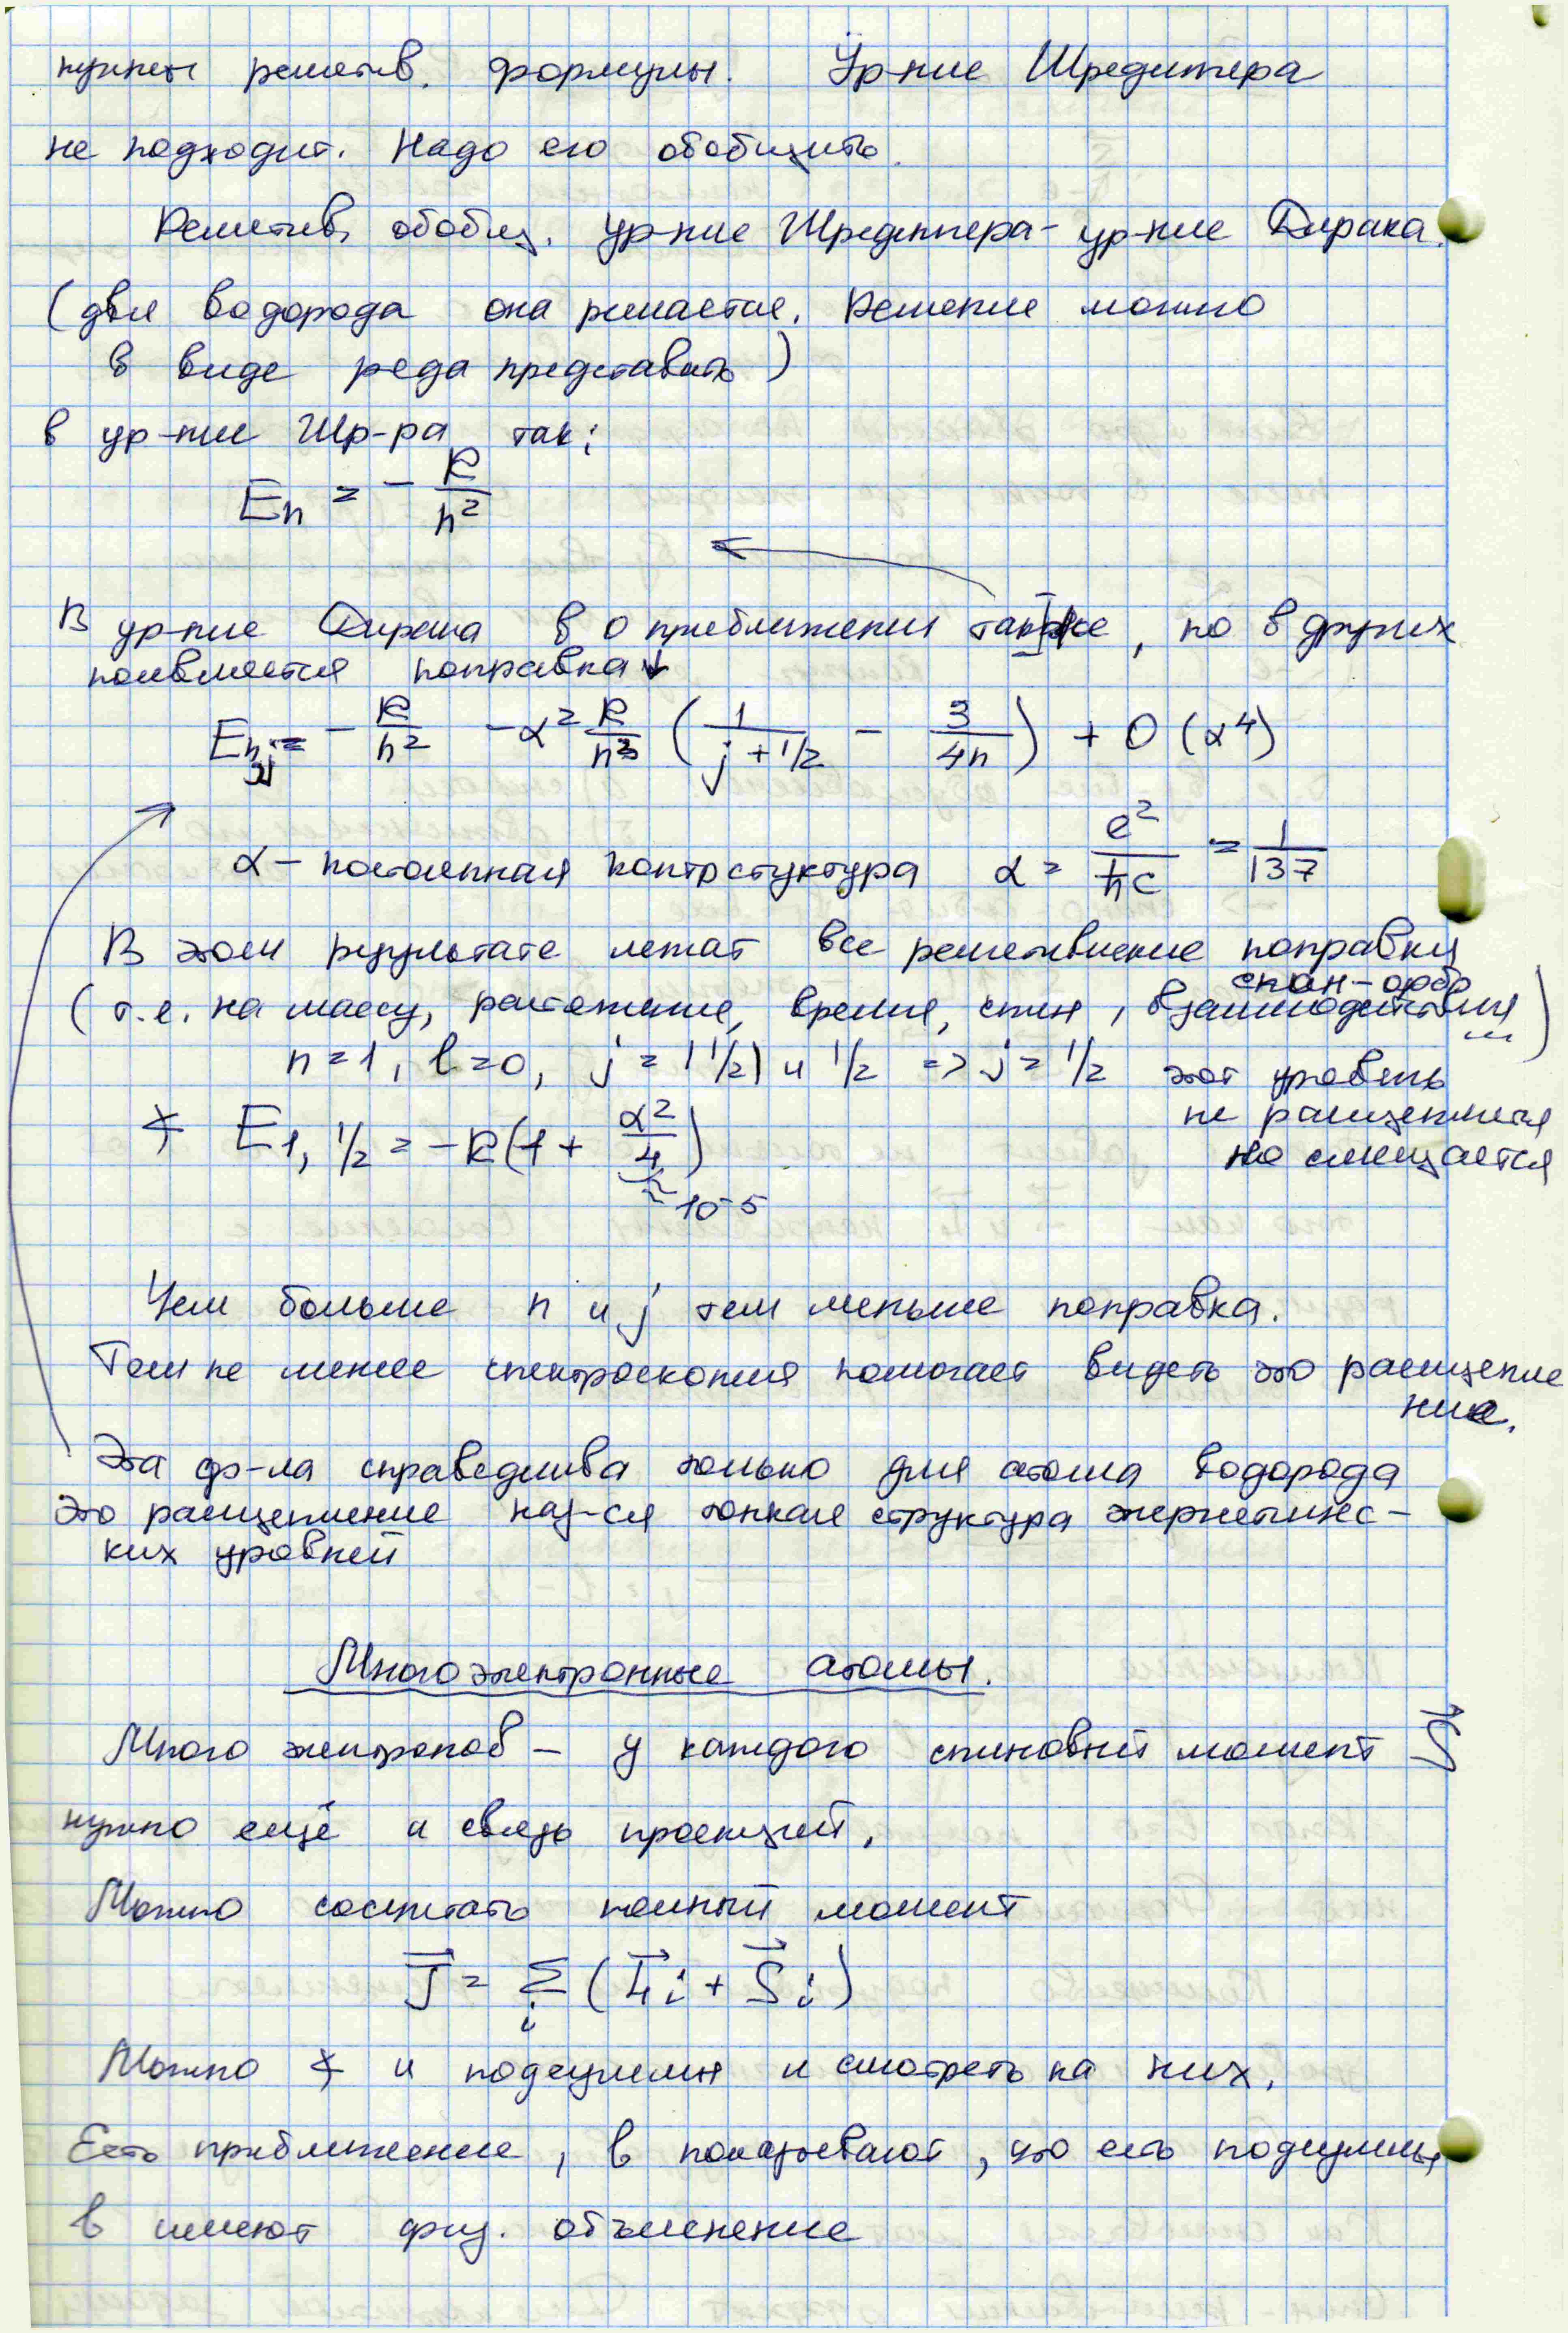
\includegraphics[max size={\textwidth}{0.995\textheight}]{jpg/1.jpg}%
\newpage%
%
%
\phantomsection\addcontentsline{toc}{subsection}{\textit{Спин-орбитальное взаимодействие многоэлектронного атома}}%
\phantomsection\addcontentsline{toc}{subsubsection}{L-S связь}%
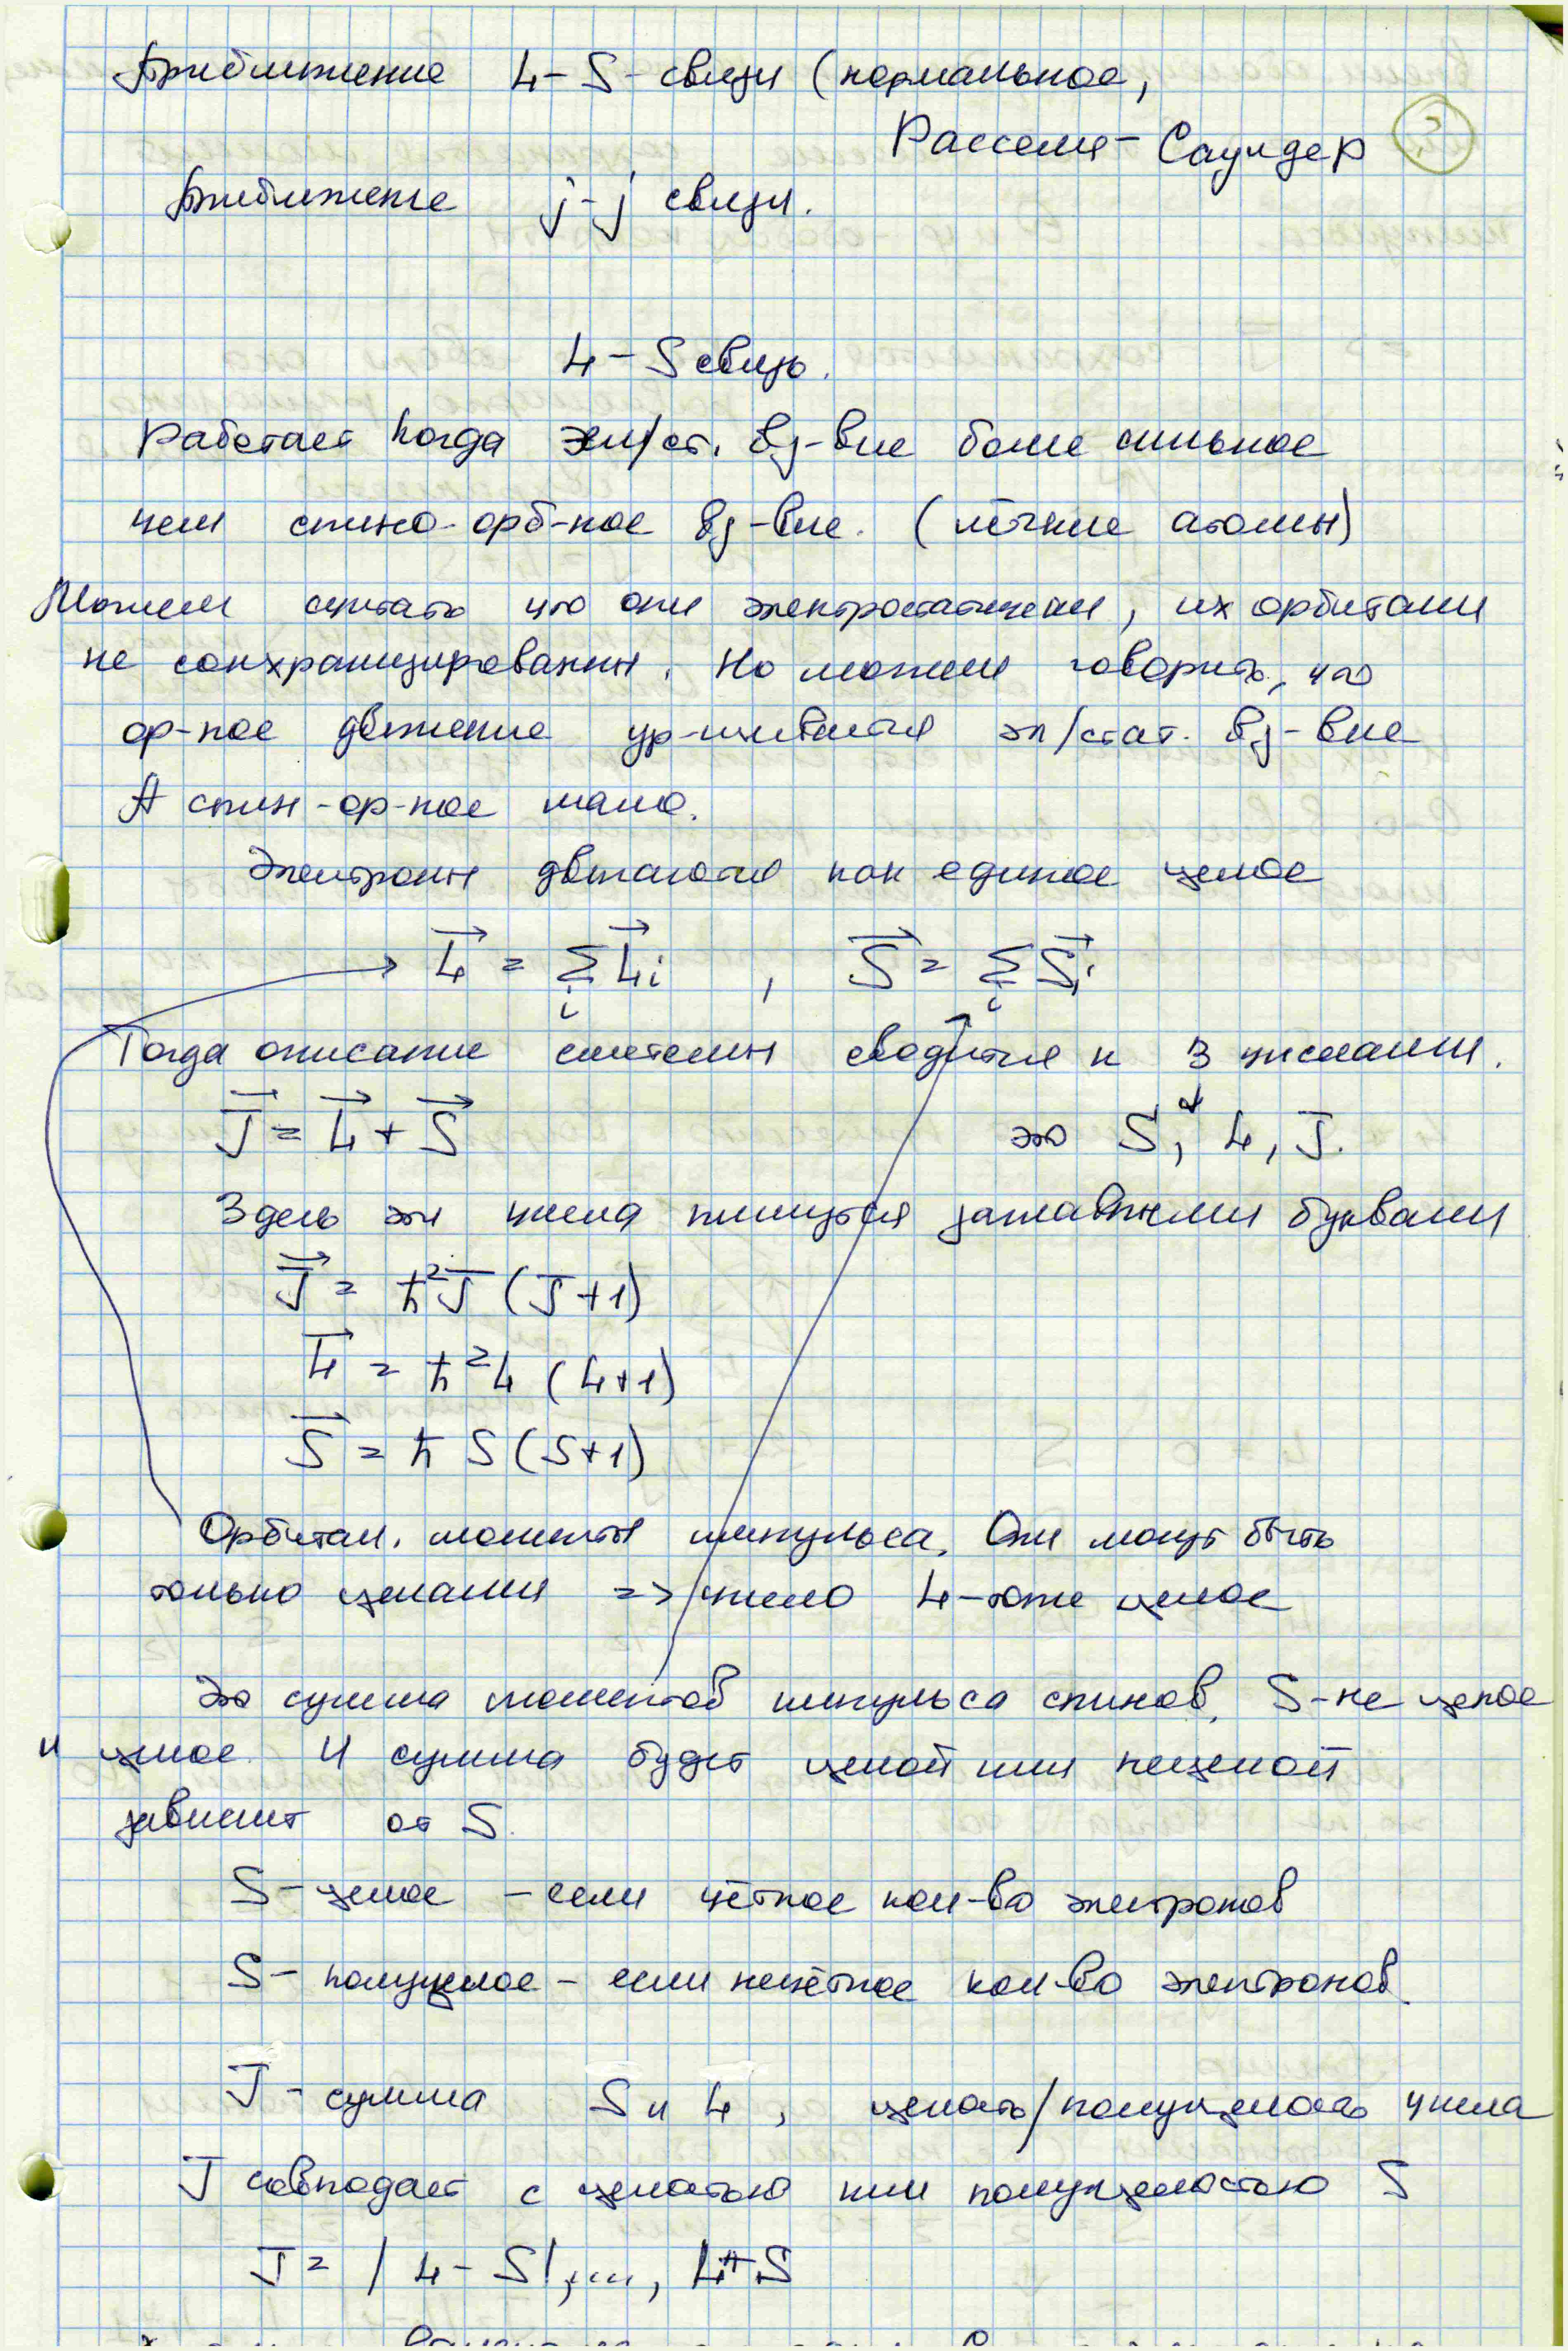
\includegraphics[max size={\textwidth}{0.995\textheight}]{jpg/2.jpg}%
\newpage%
%
%
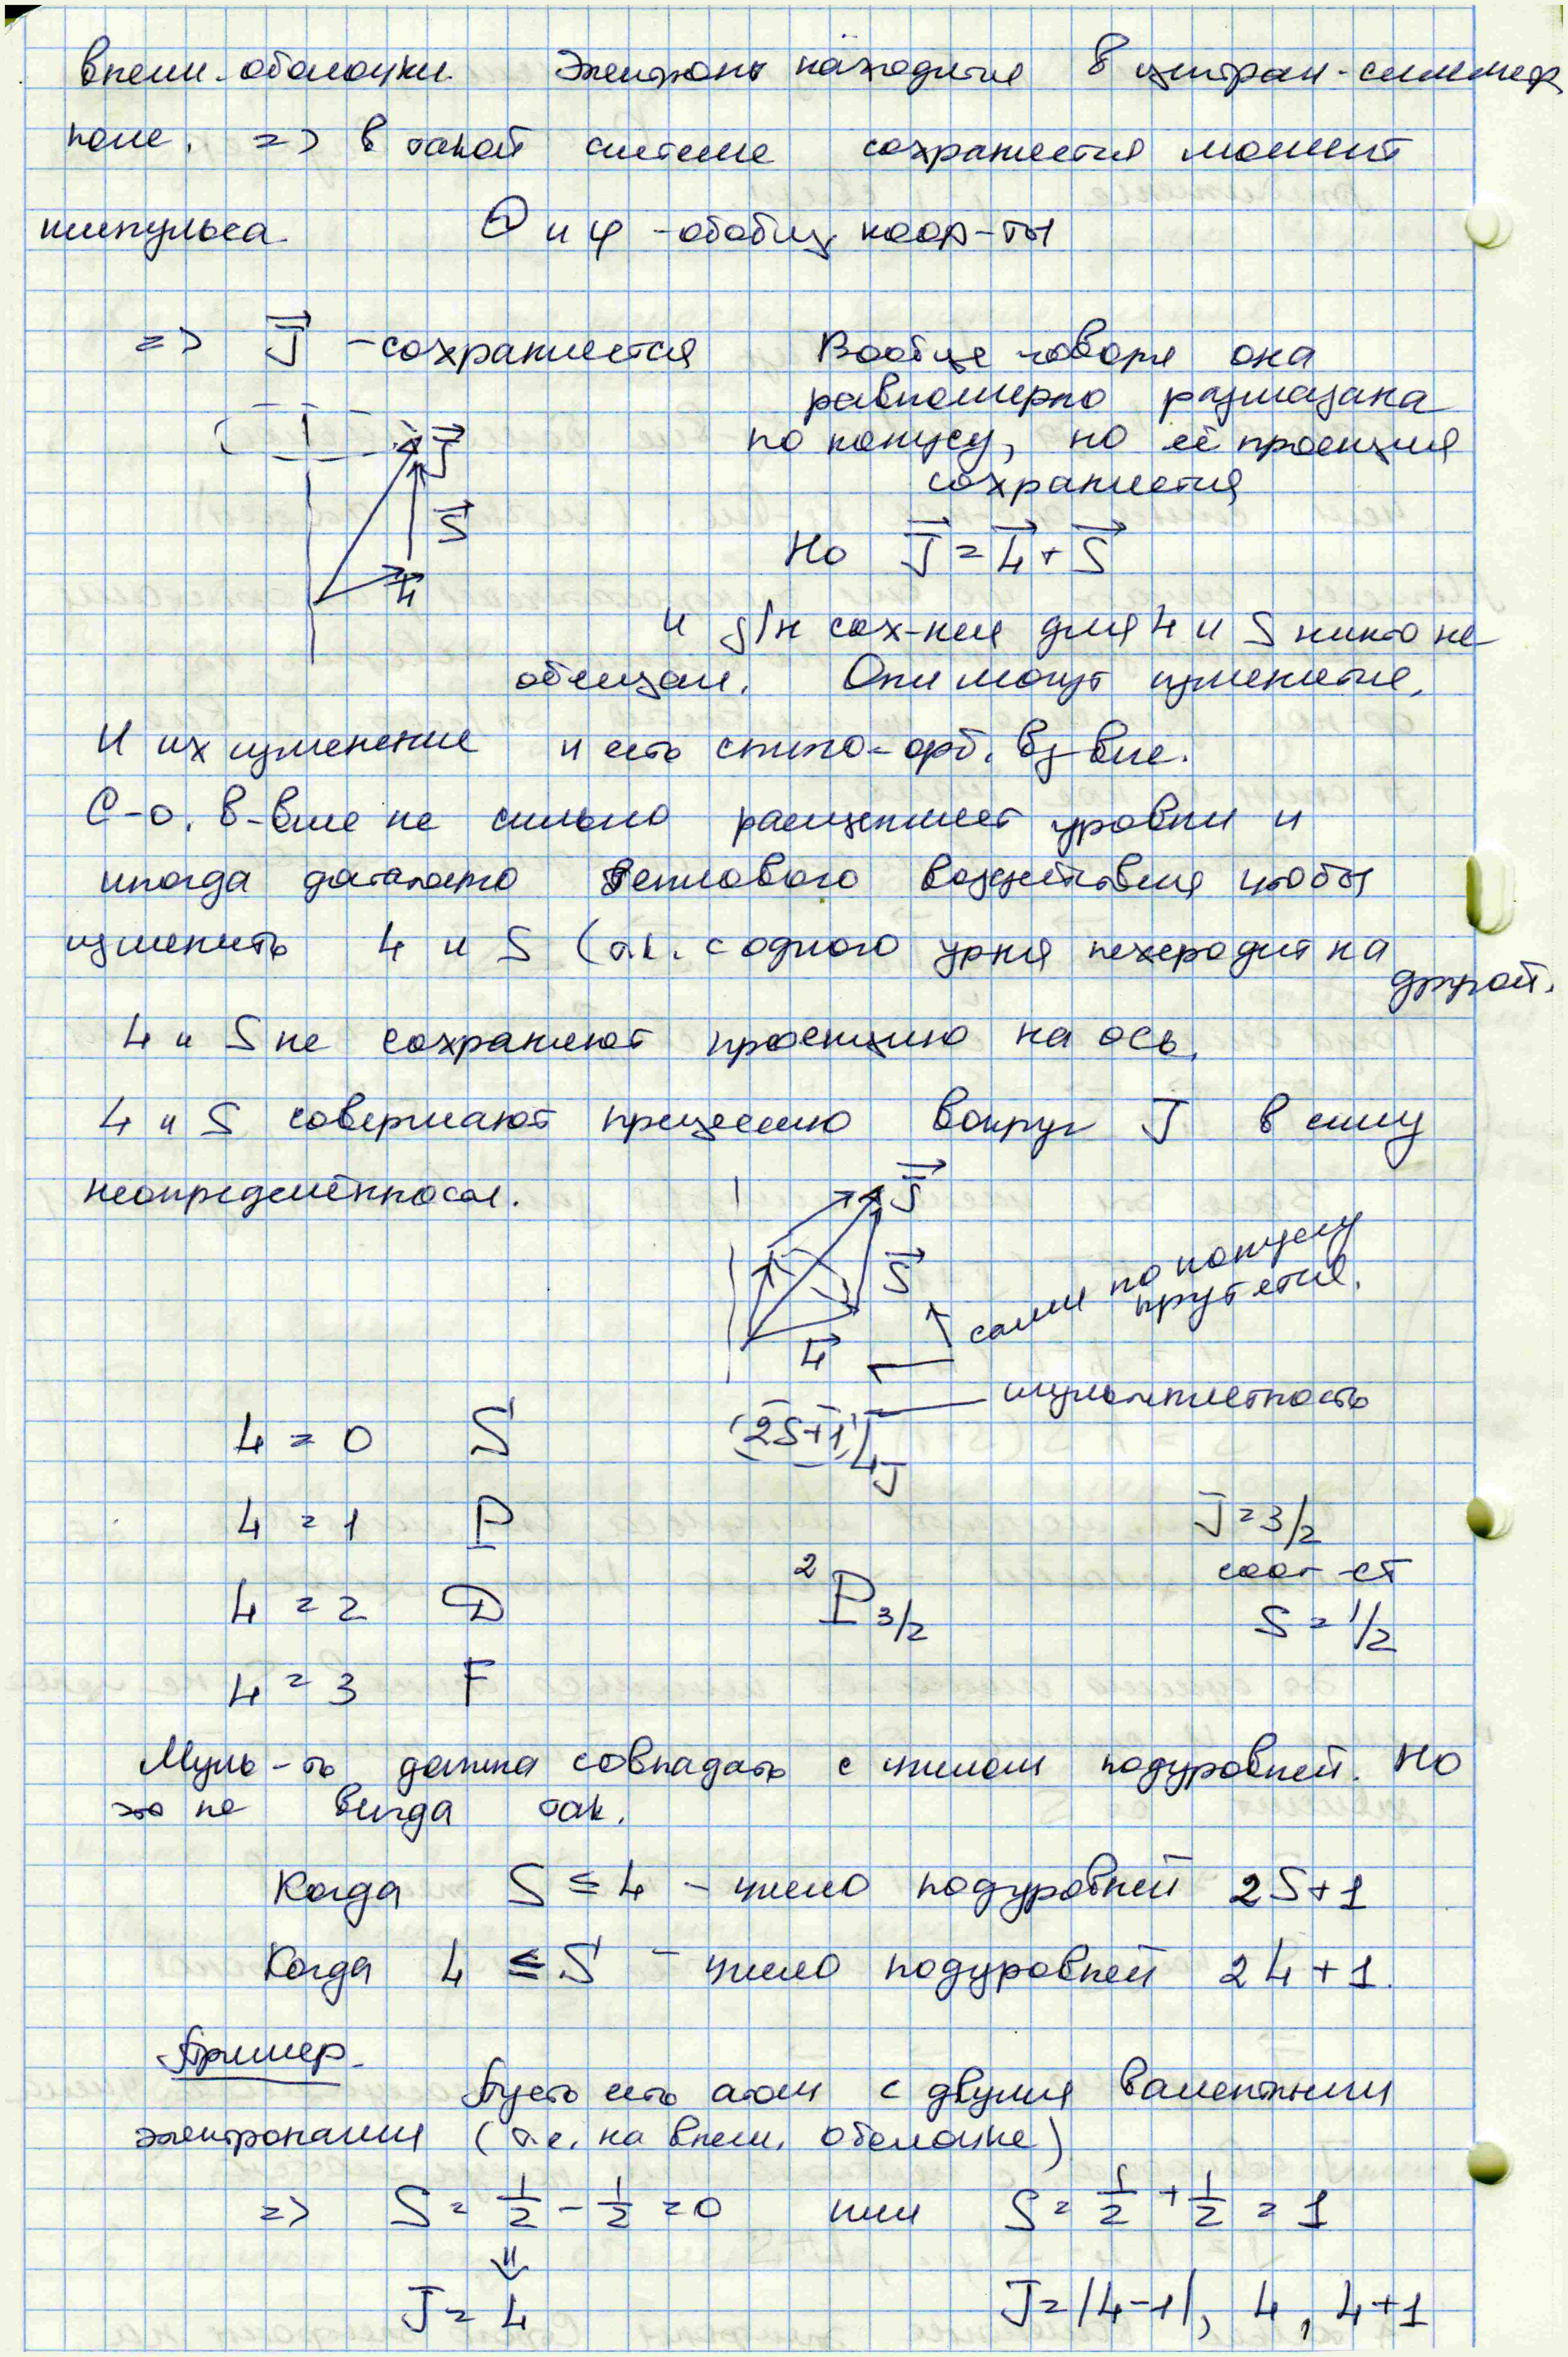
\includegraphics[max size={\textwidth}{0.995\textheight}]{jpg/3.jpg}%
\newpage%
%
%
\phantomsection\addcontentsline{toc}{subsubsection}{j-j связь}%
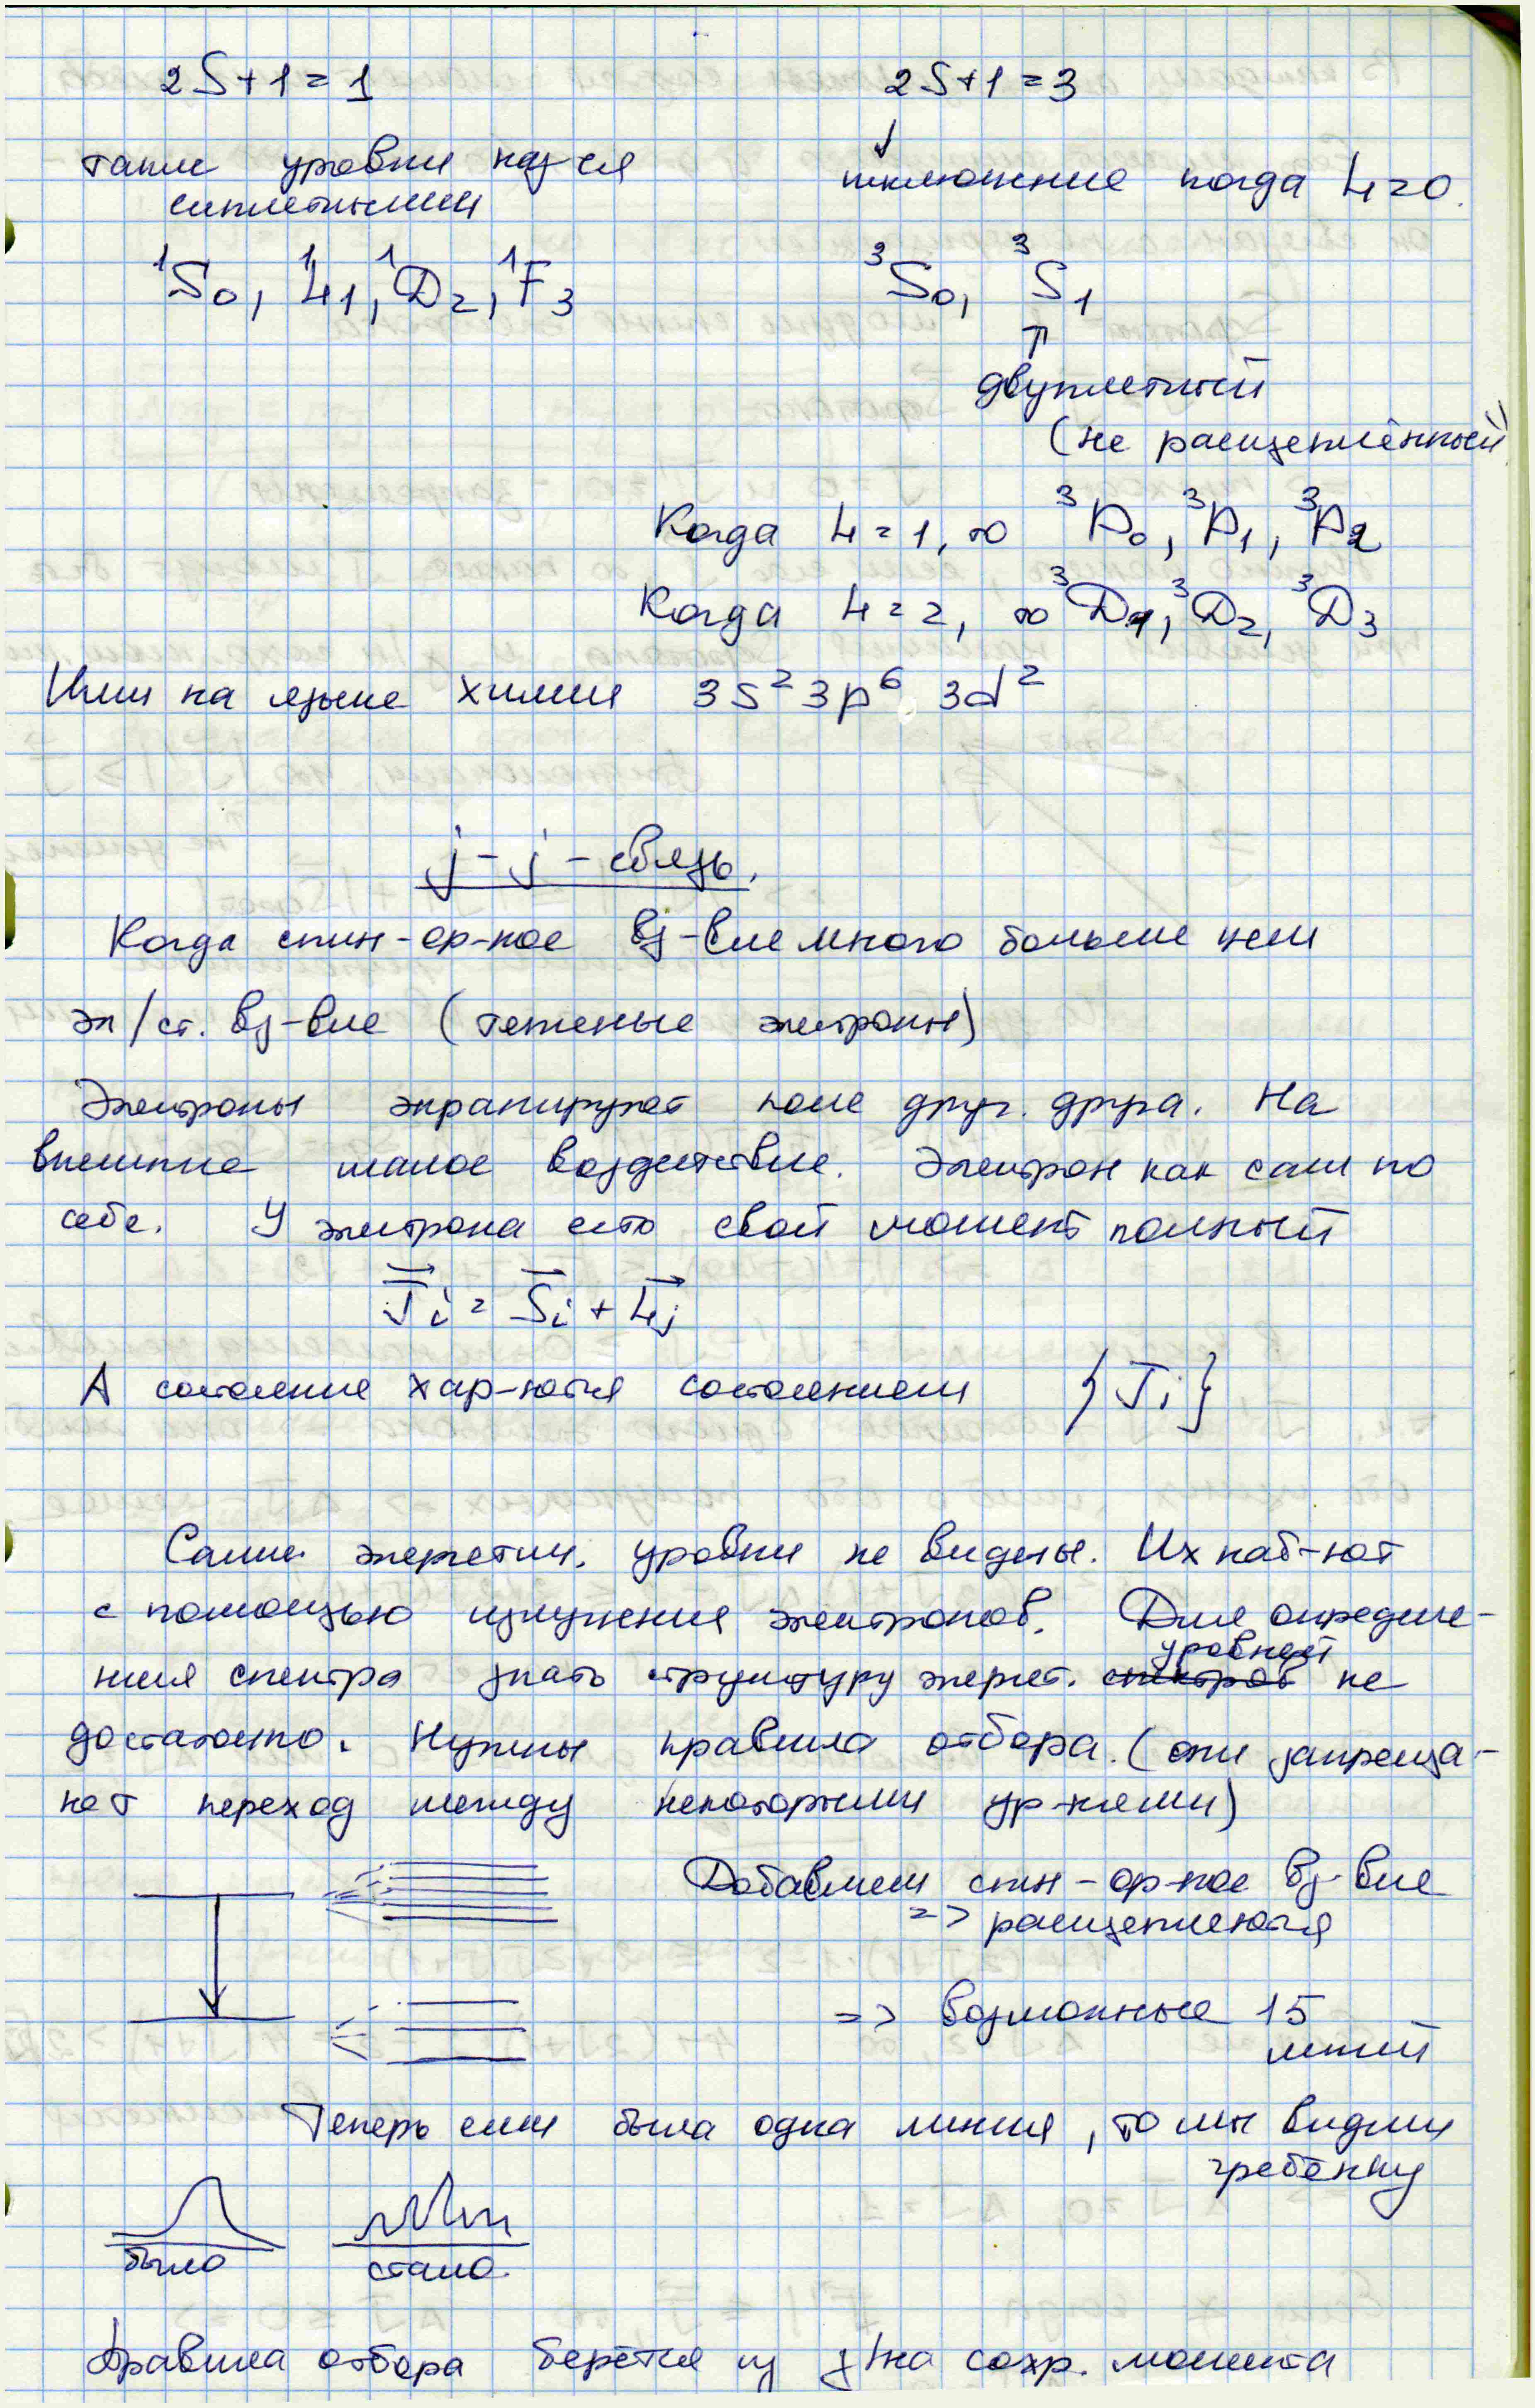
\includegraphics[max size={\textwidth}{0.995\textheight}]{jpg/4.jpg}%
\newpage%
%
%
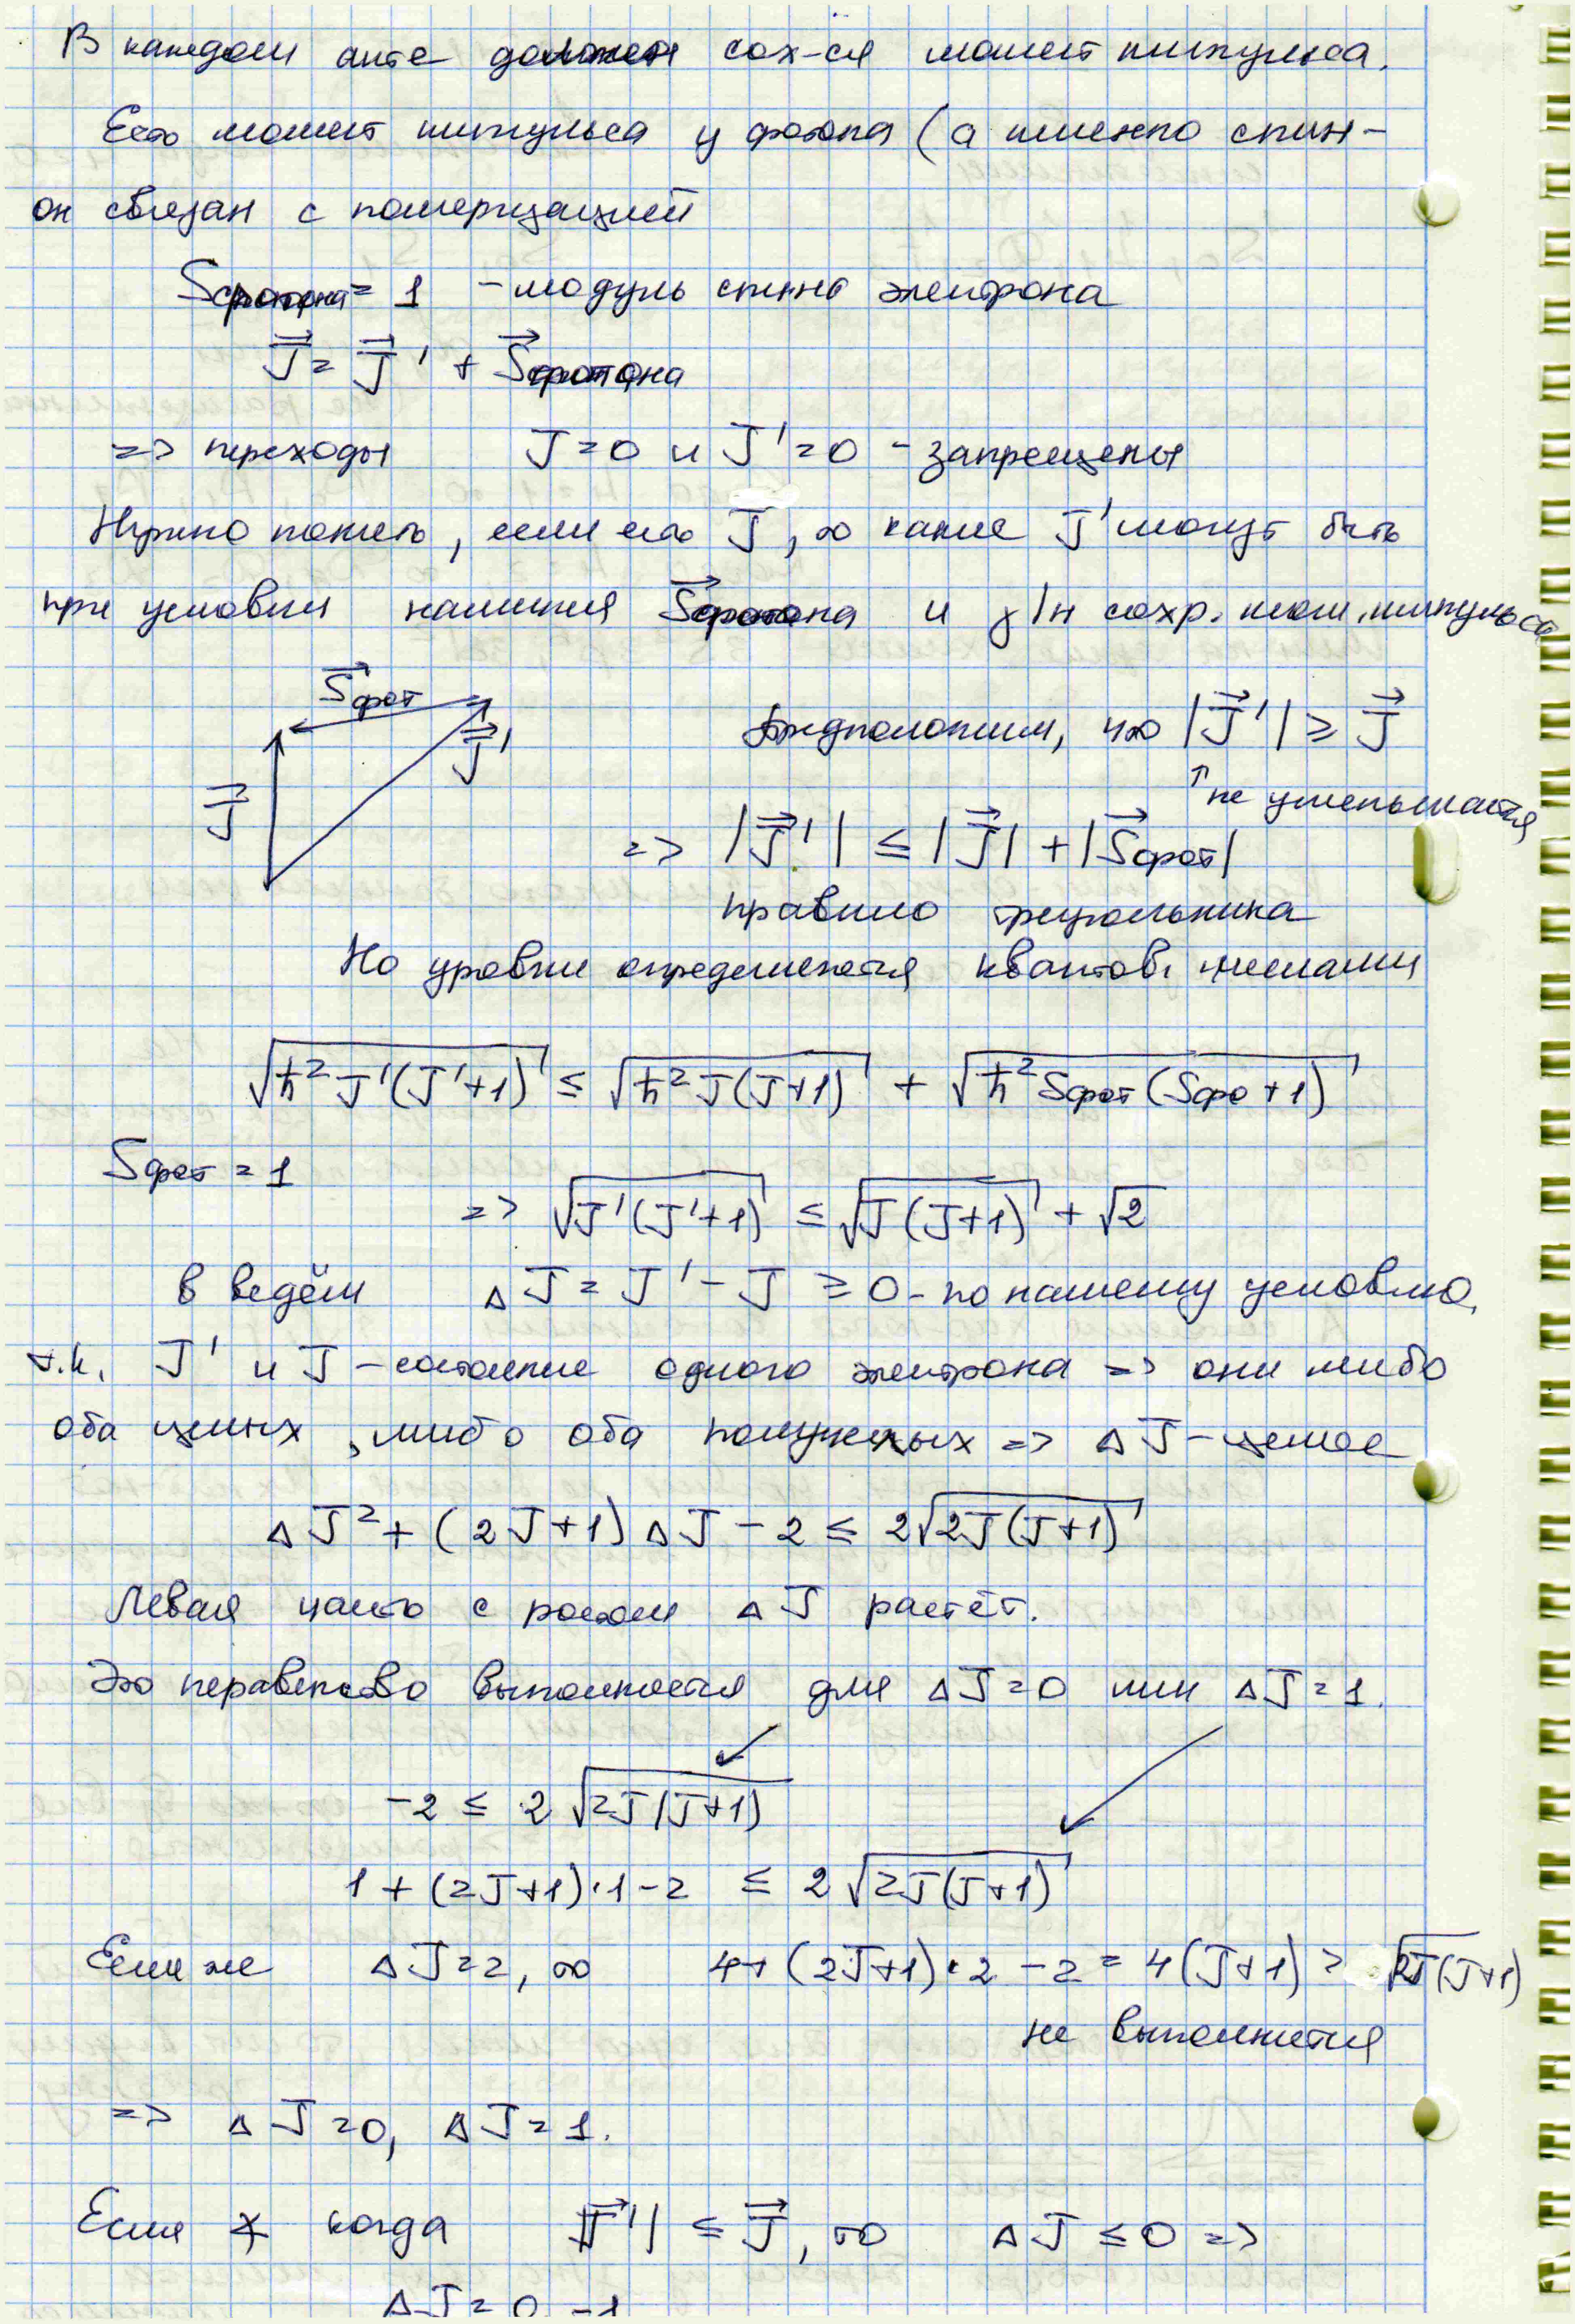
\includegraphics[max size={\textwidth}{0.995\textheight}]{jpg/5.jpg}%
\newpage%
%
%
\phantomsection\addcontentsline{toc}{subsection}{Правила отбора}%
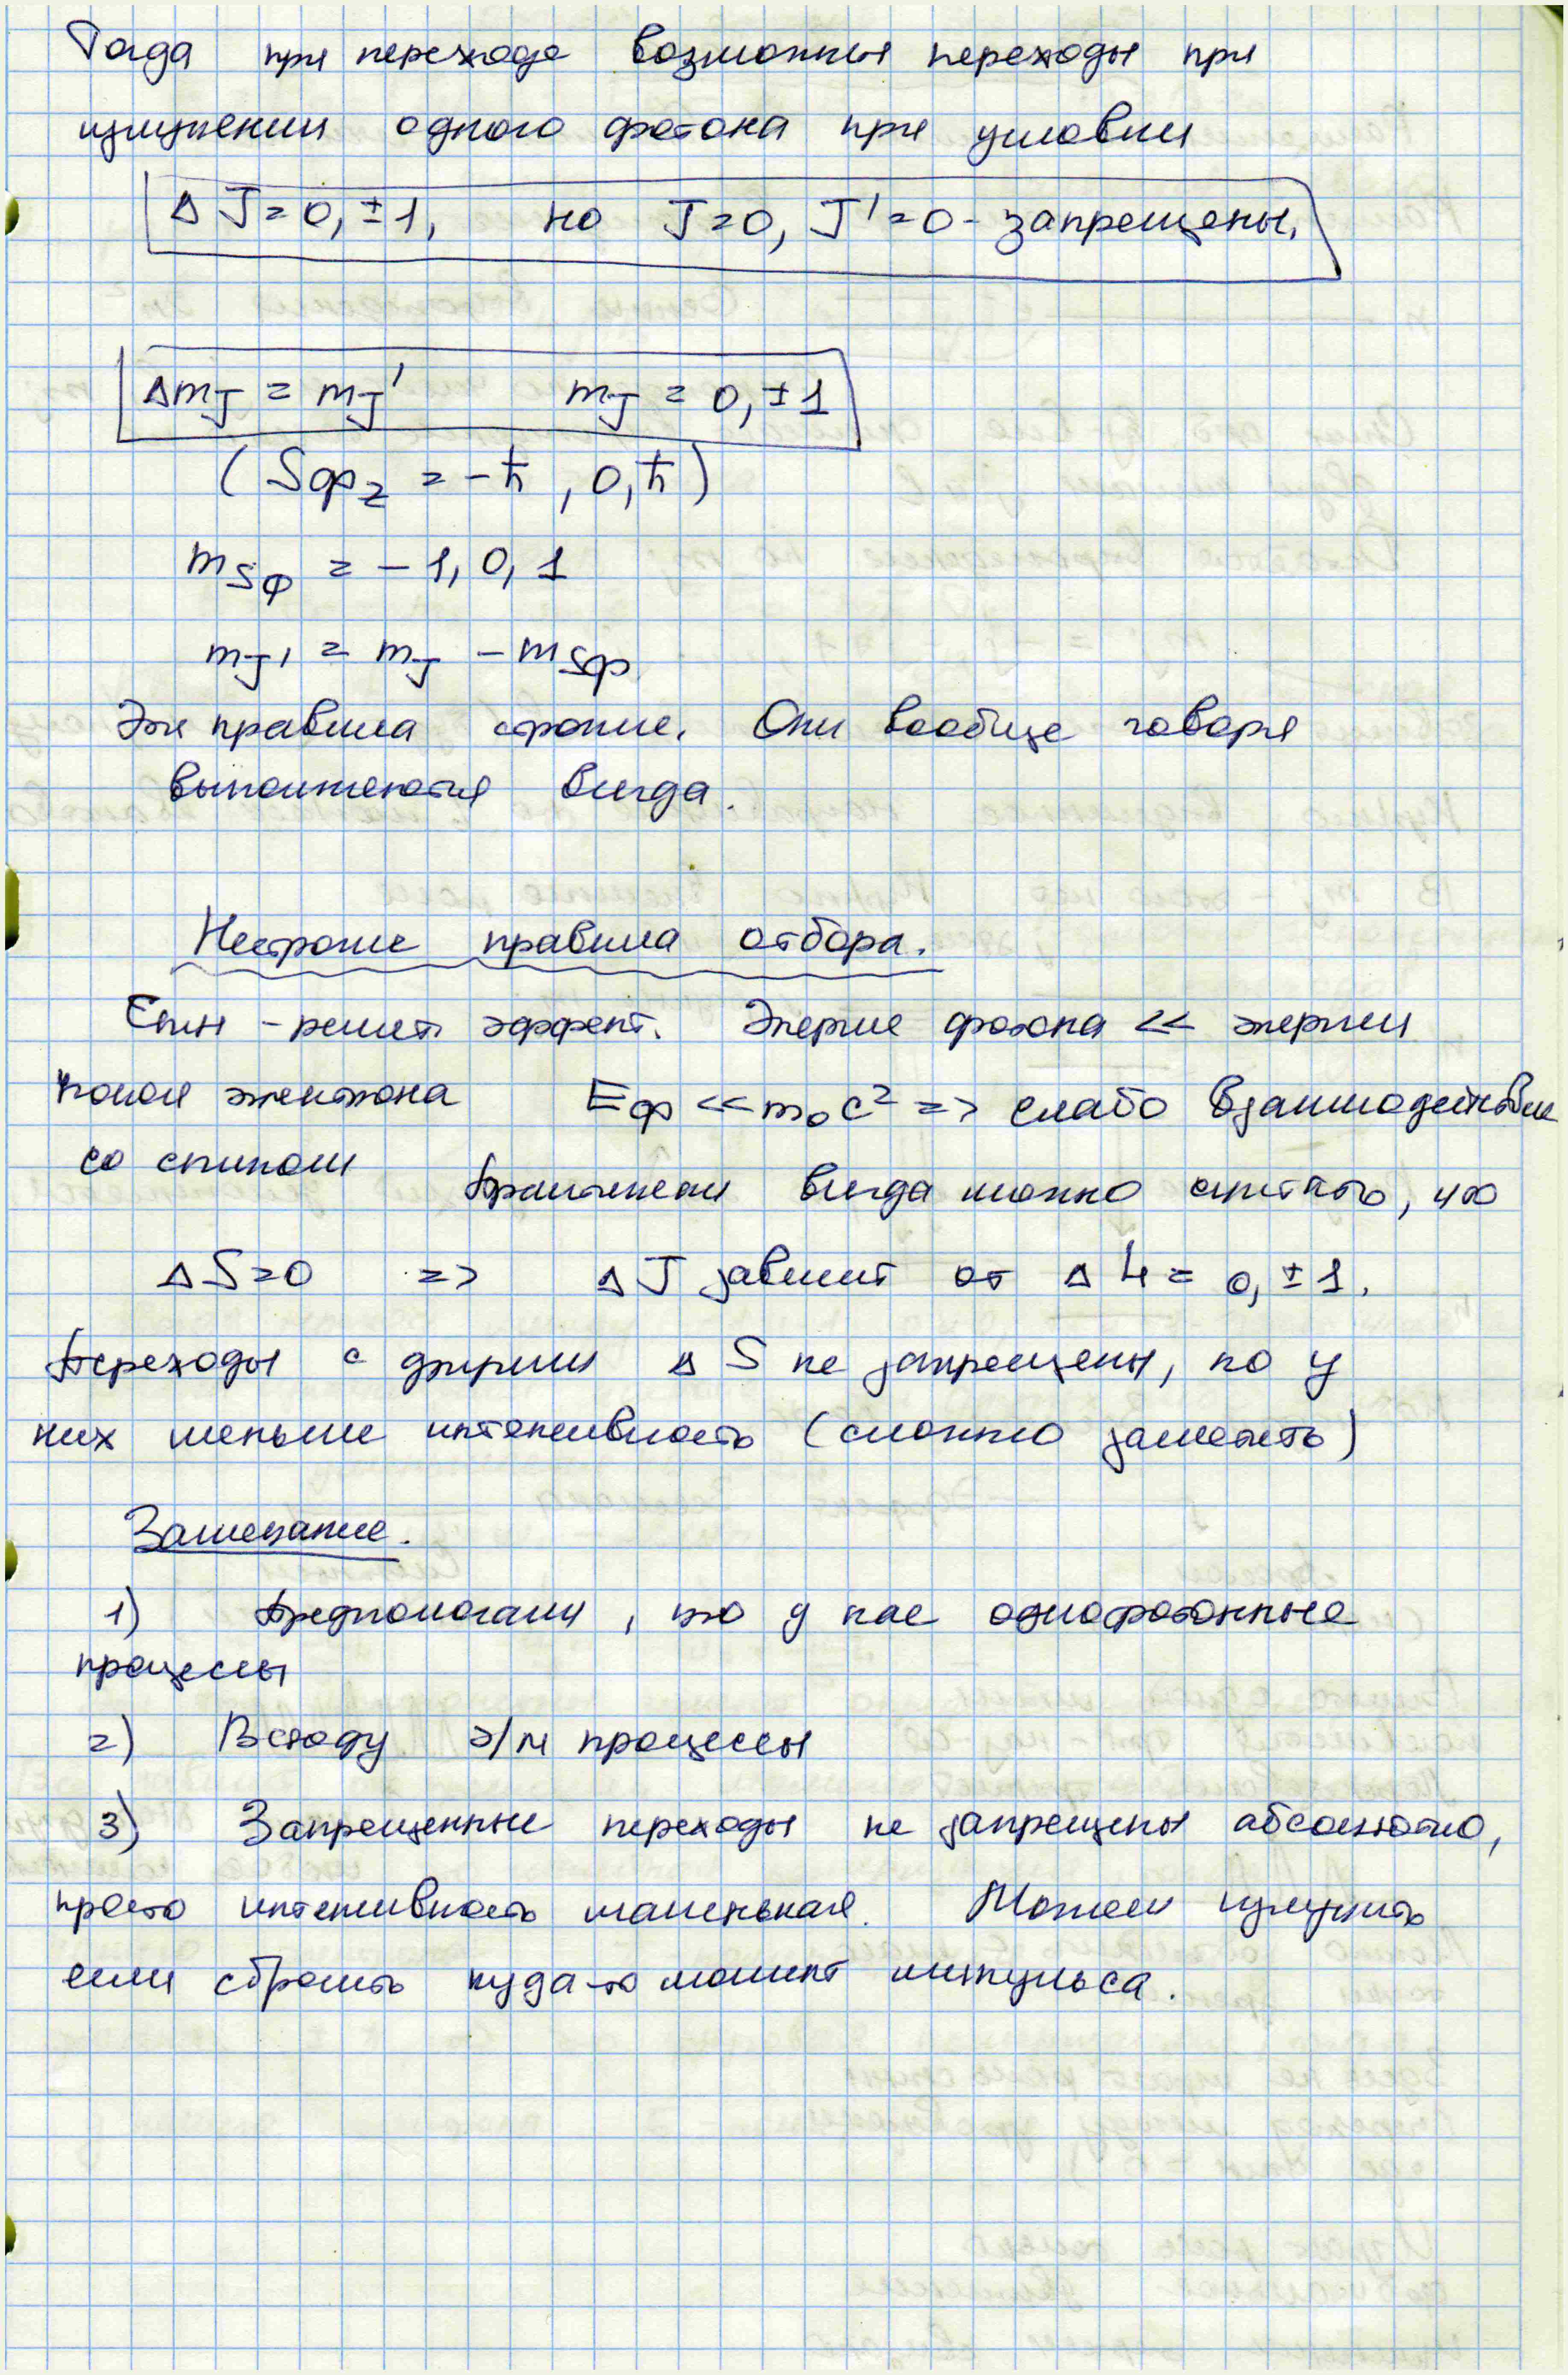
\includegraphics[max size={\textwidth}{0.995\textheight}]{jpg/6.jpg}%
\newpage%
%
%
\phantomsection\addcontentsline{toc}{subsection}{Эффект Зеемана}%
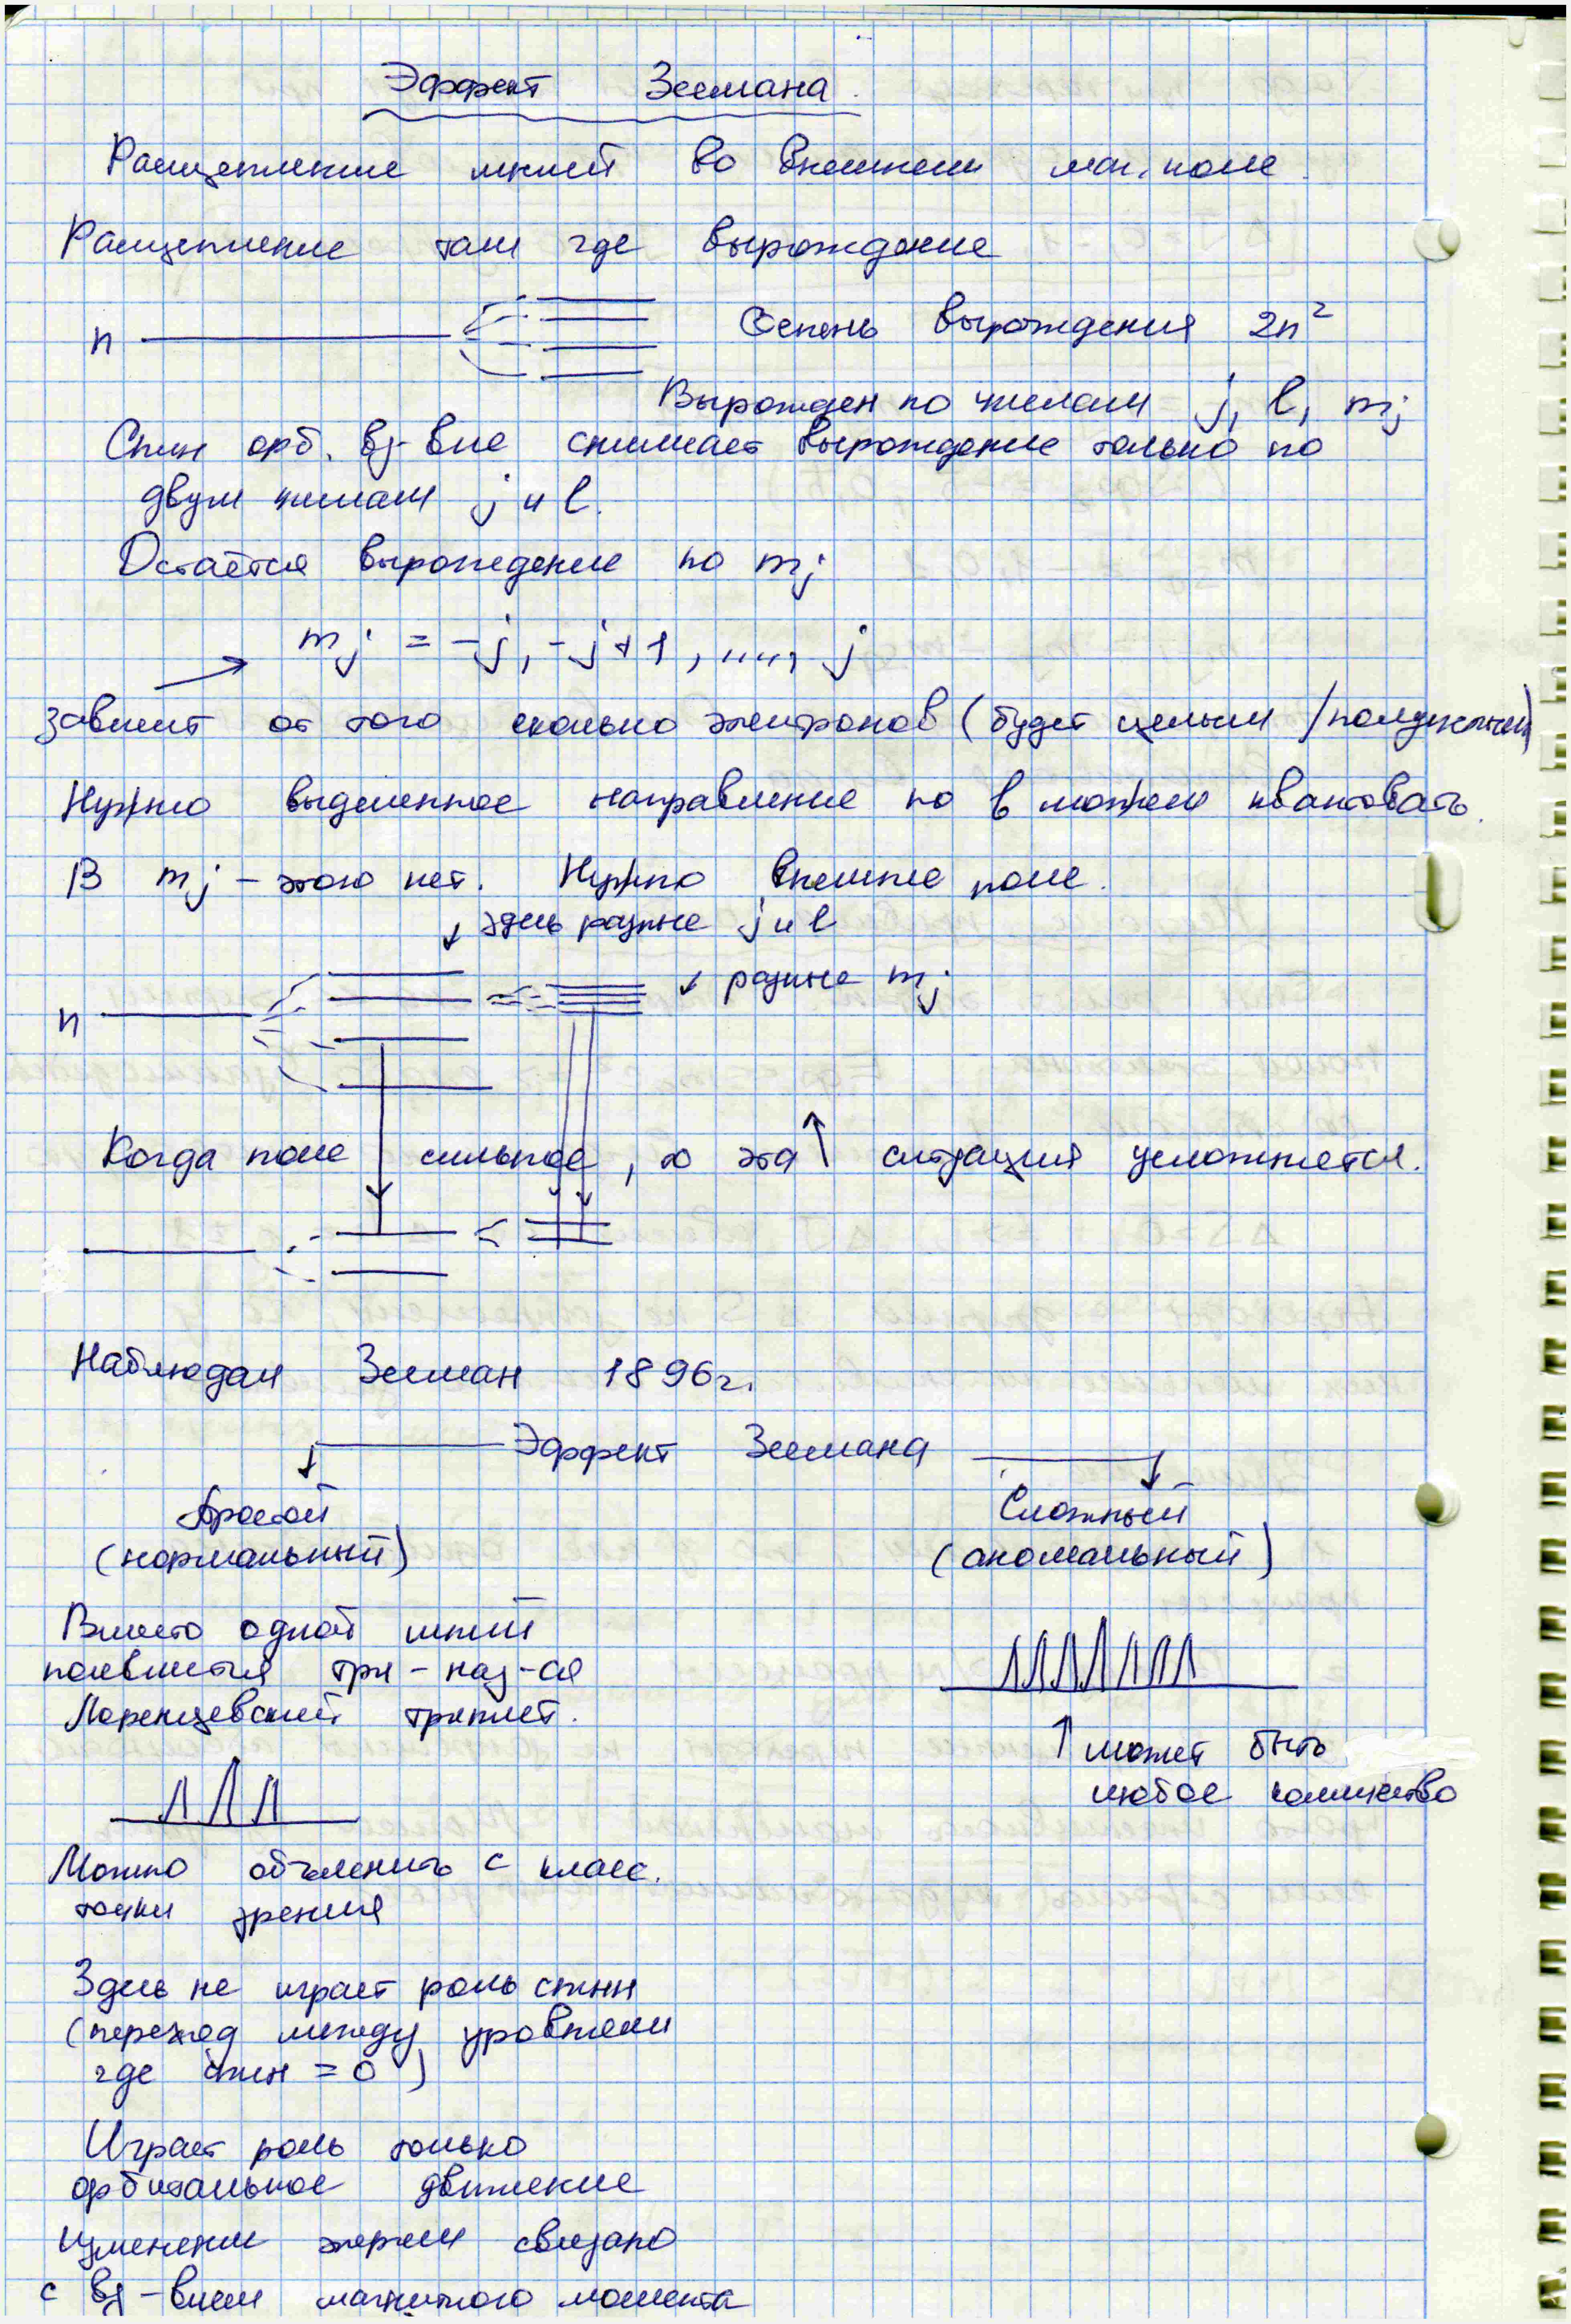
\includegraphics[max size={\textwidth}{0.995\textheight}]{jpg/7.jpg}%
\newpage%
%
%
\phantomsection\addcontentsline{toc}{subsubsection}{Простой эффект Зеемана}%
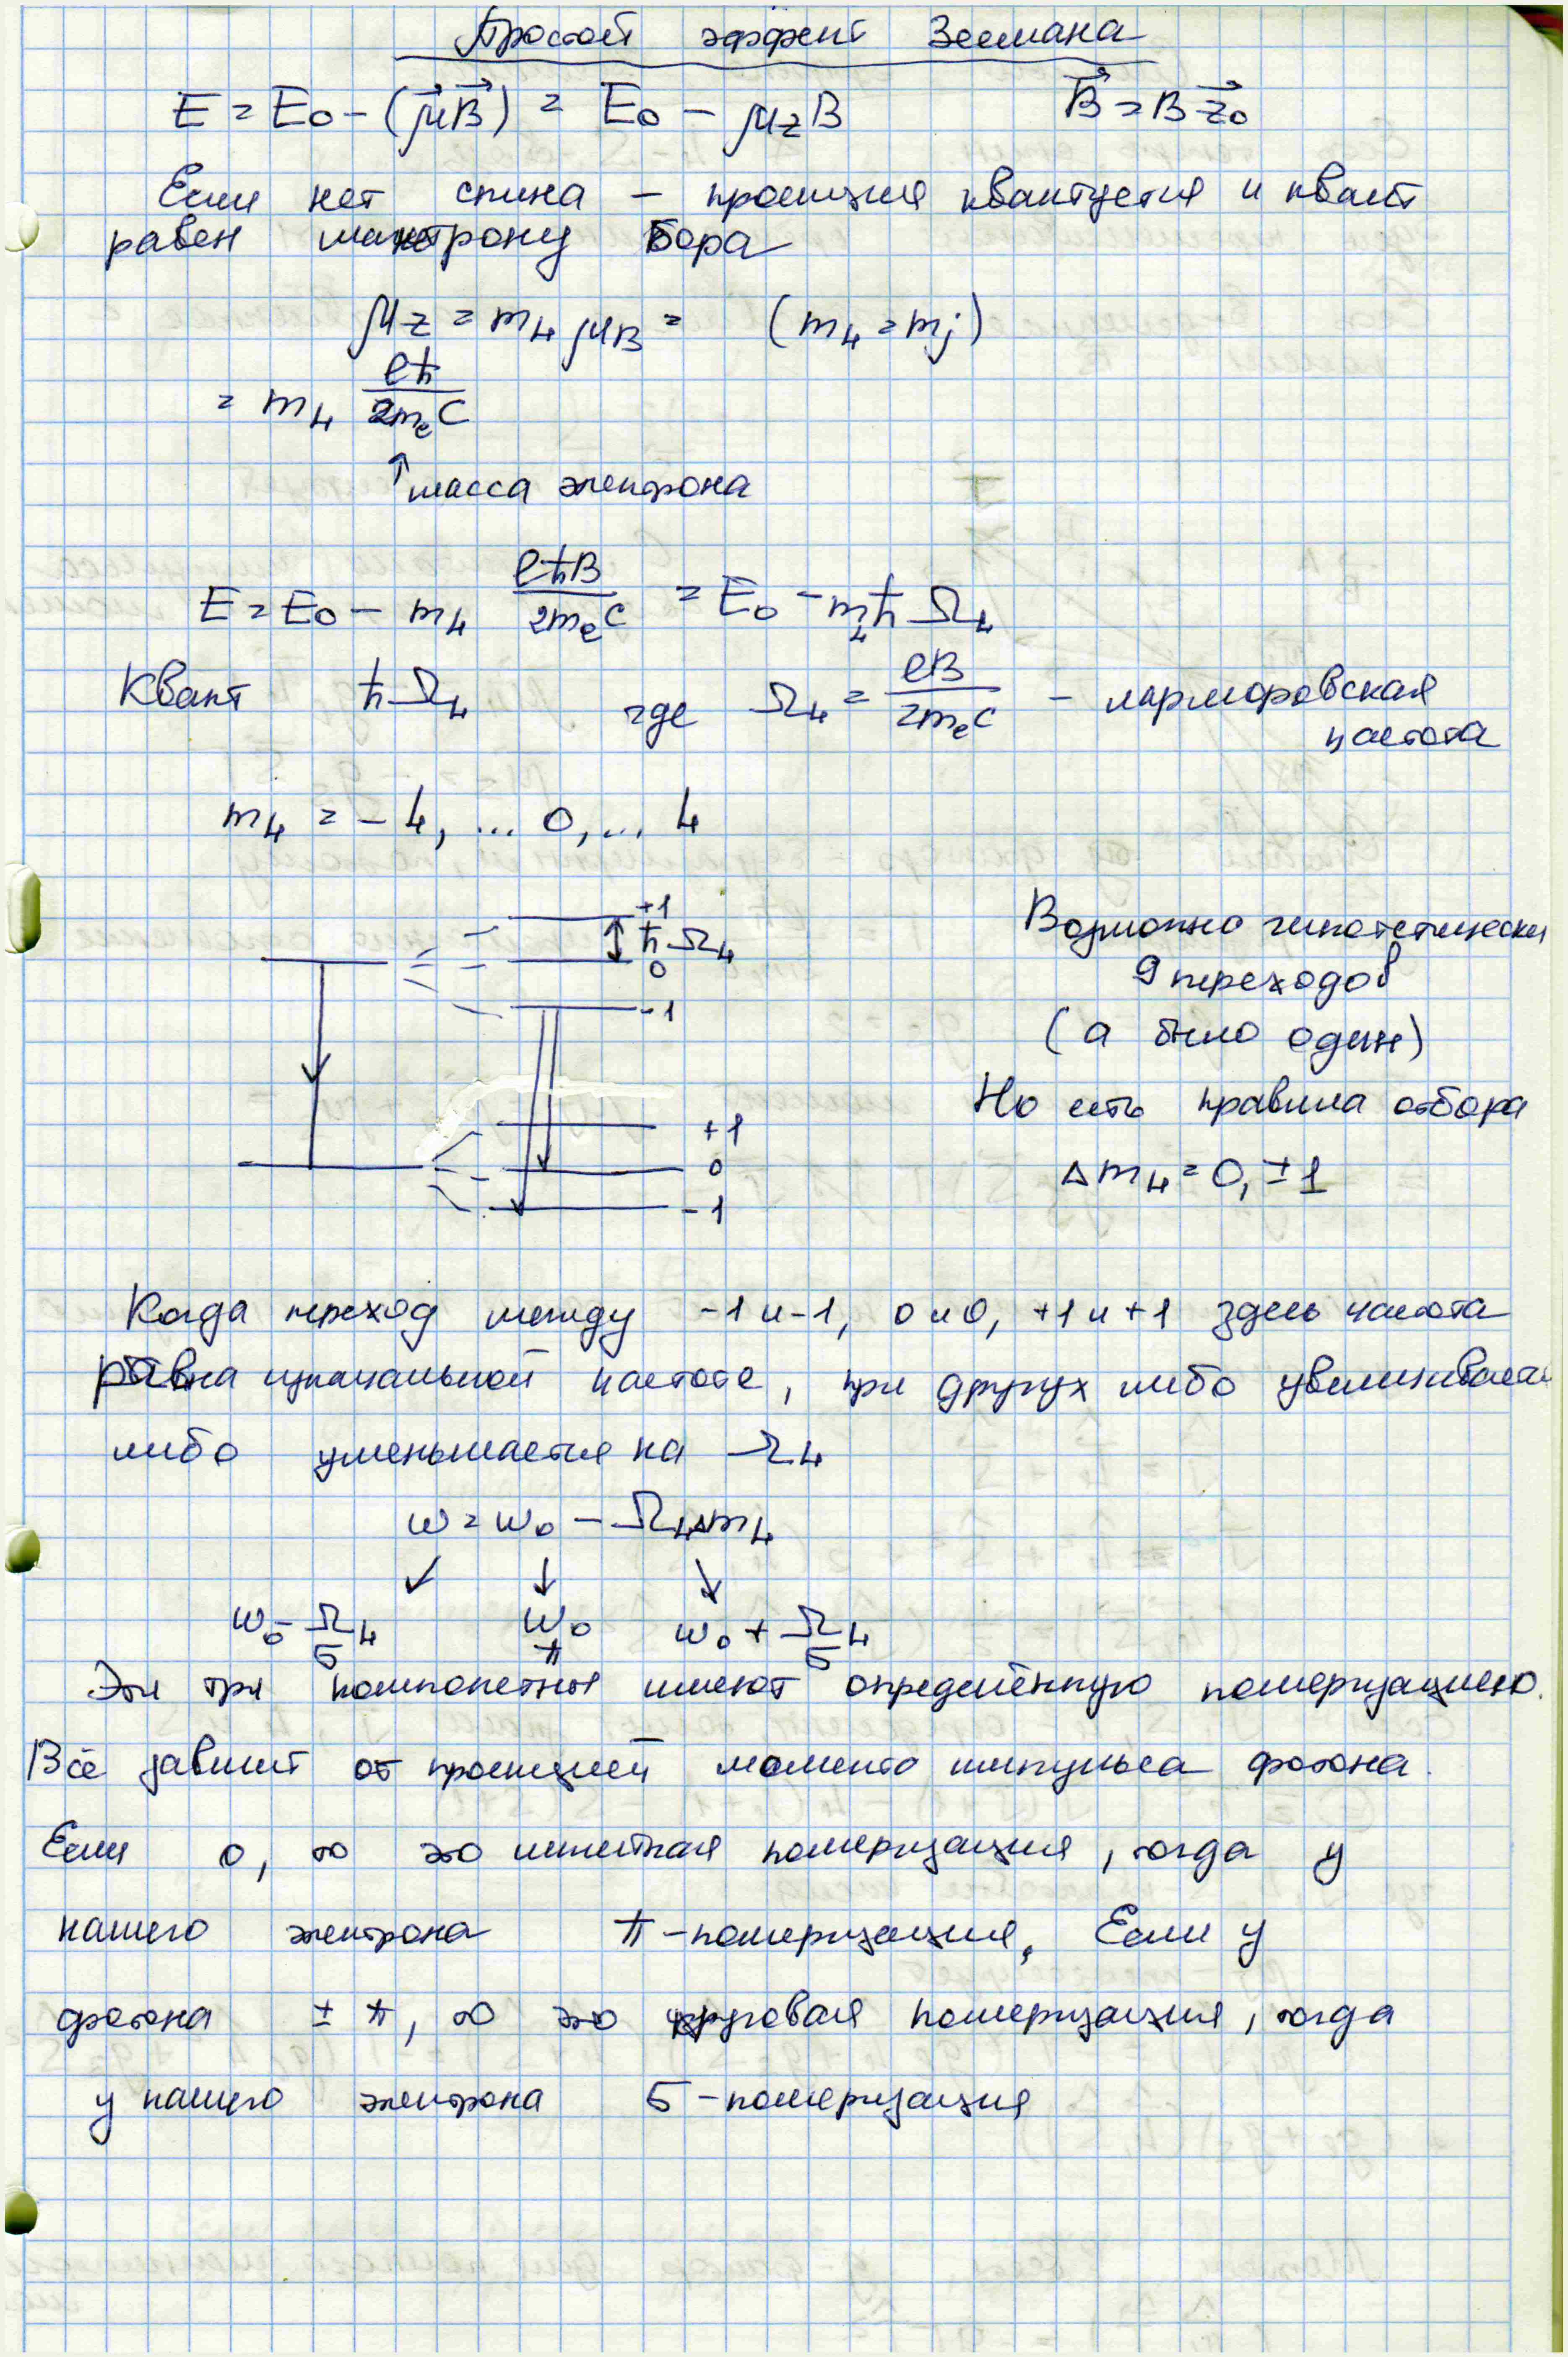
\includegraphics[max size={\textwidth}{0.995\textheight}]{jpg/8.jpg}%
\newpage%
%
%
\phantomsection\addcontentsline{toc}{subsubsection}{Сложный эффект Зеемана}%
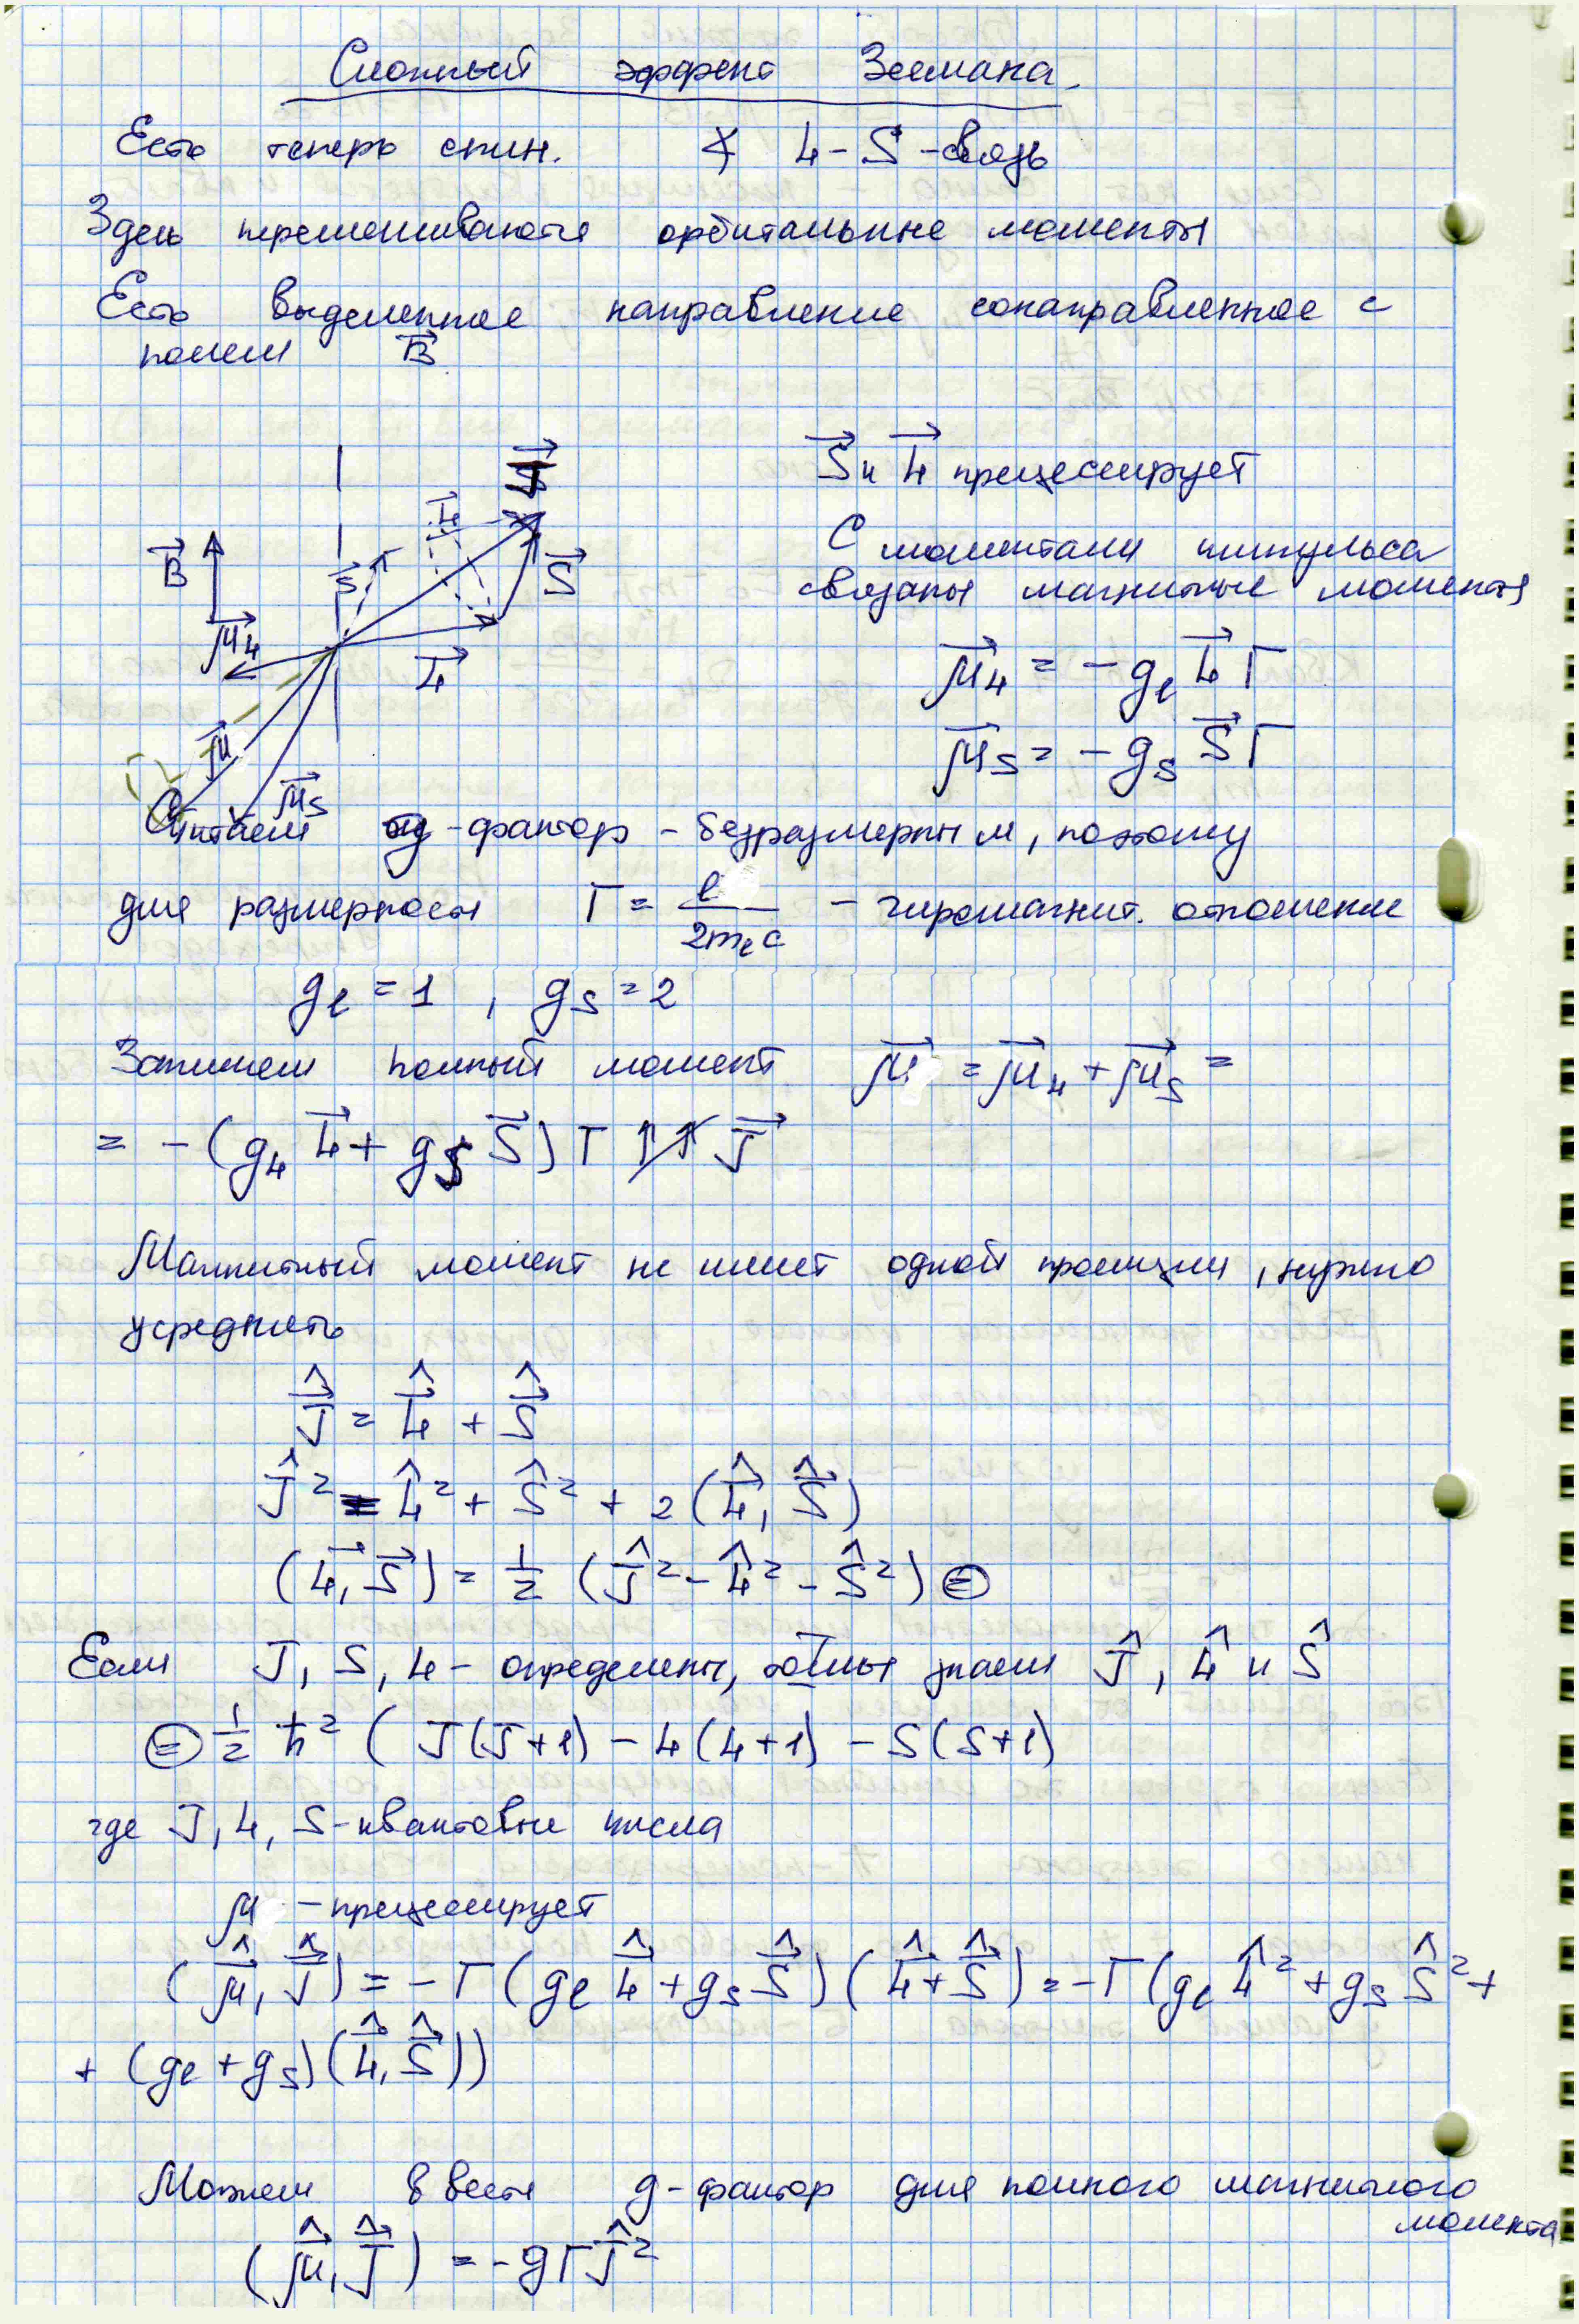
\includegraphics[max size={\textwidth}{0.995\textheight}]{jpg/9.jpg}%
\newpage%
%
%
\phantomsection\addcontentsline{toc}{subsection}{Эффект Пашена-Бака}%
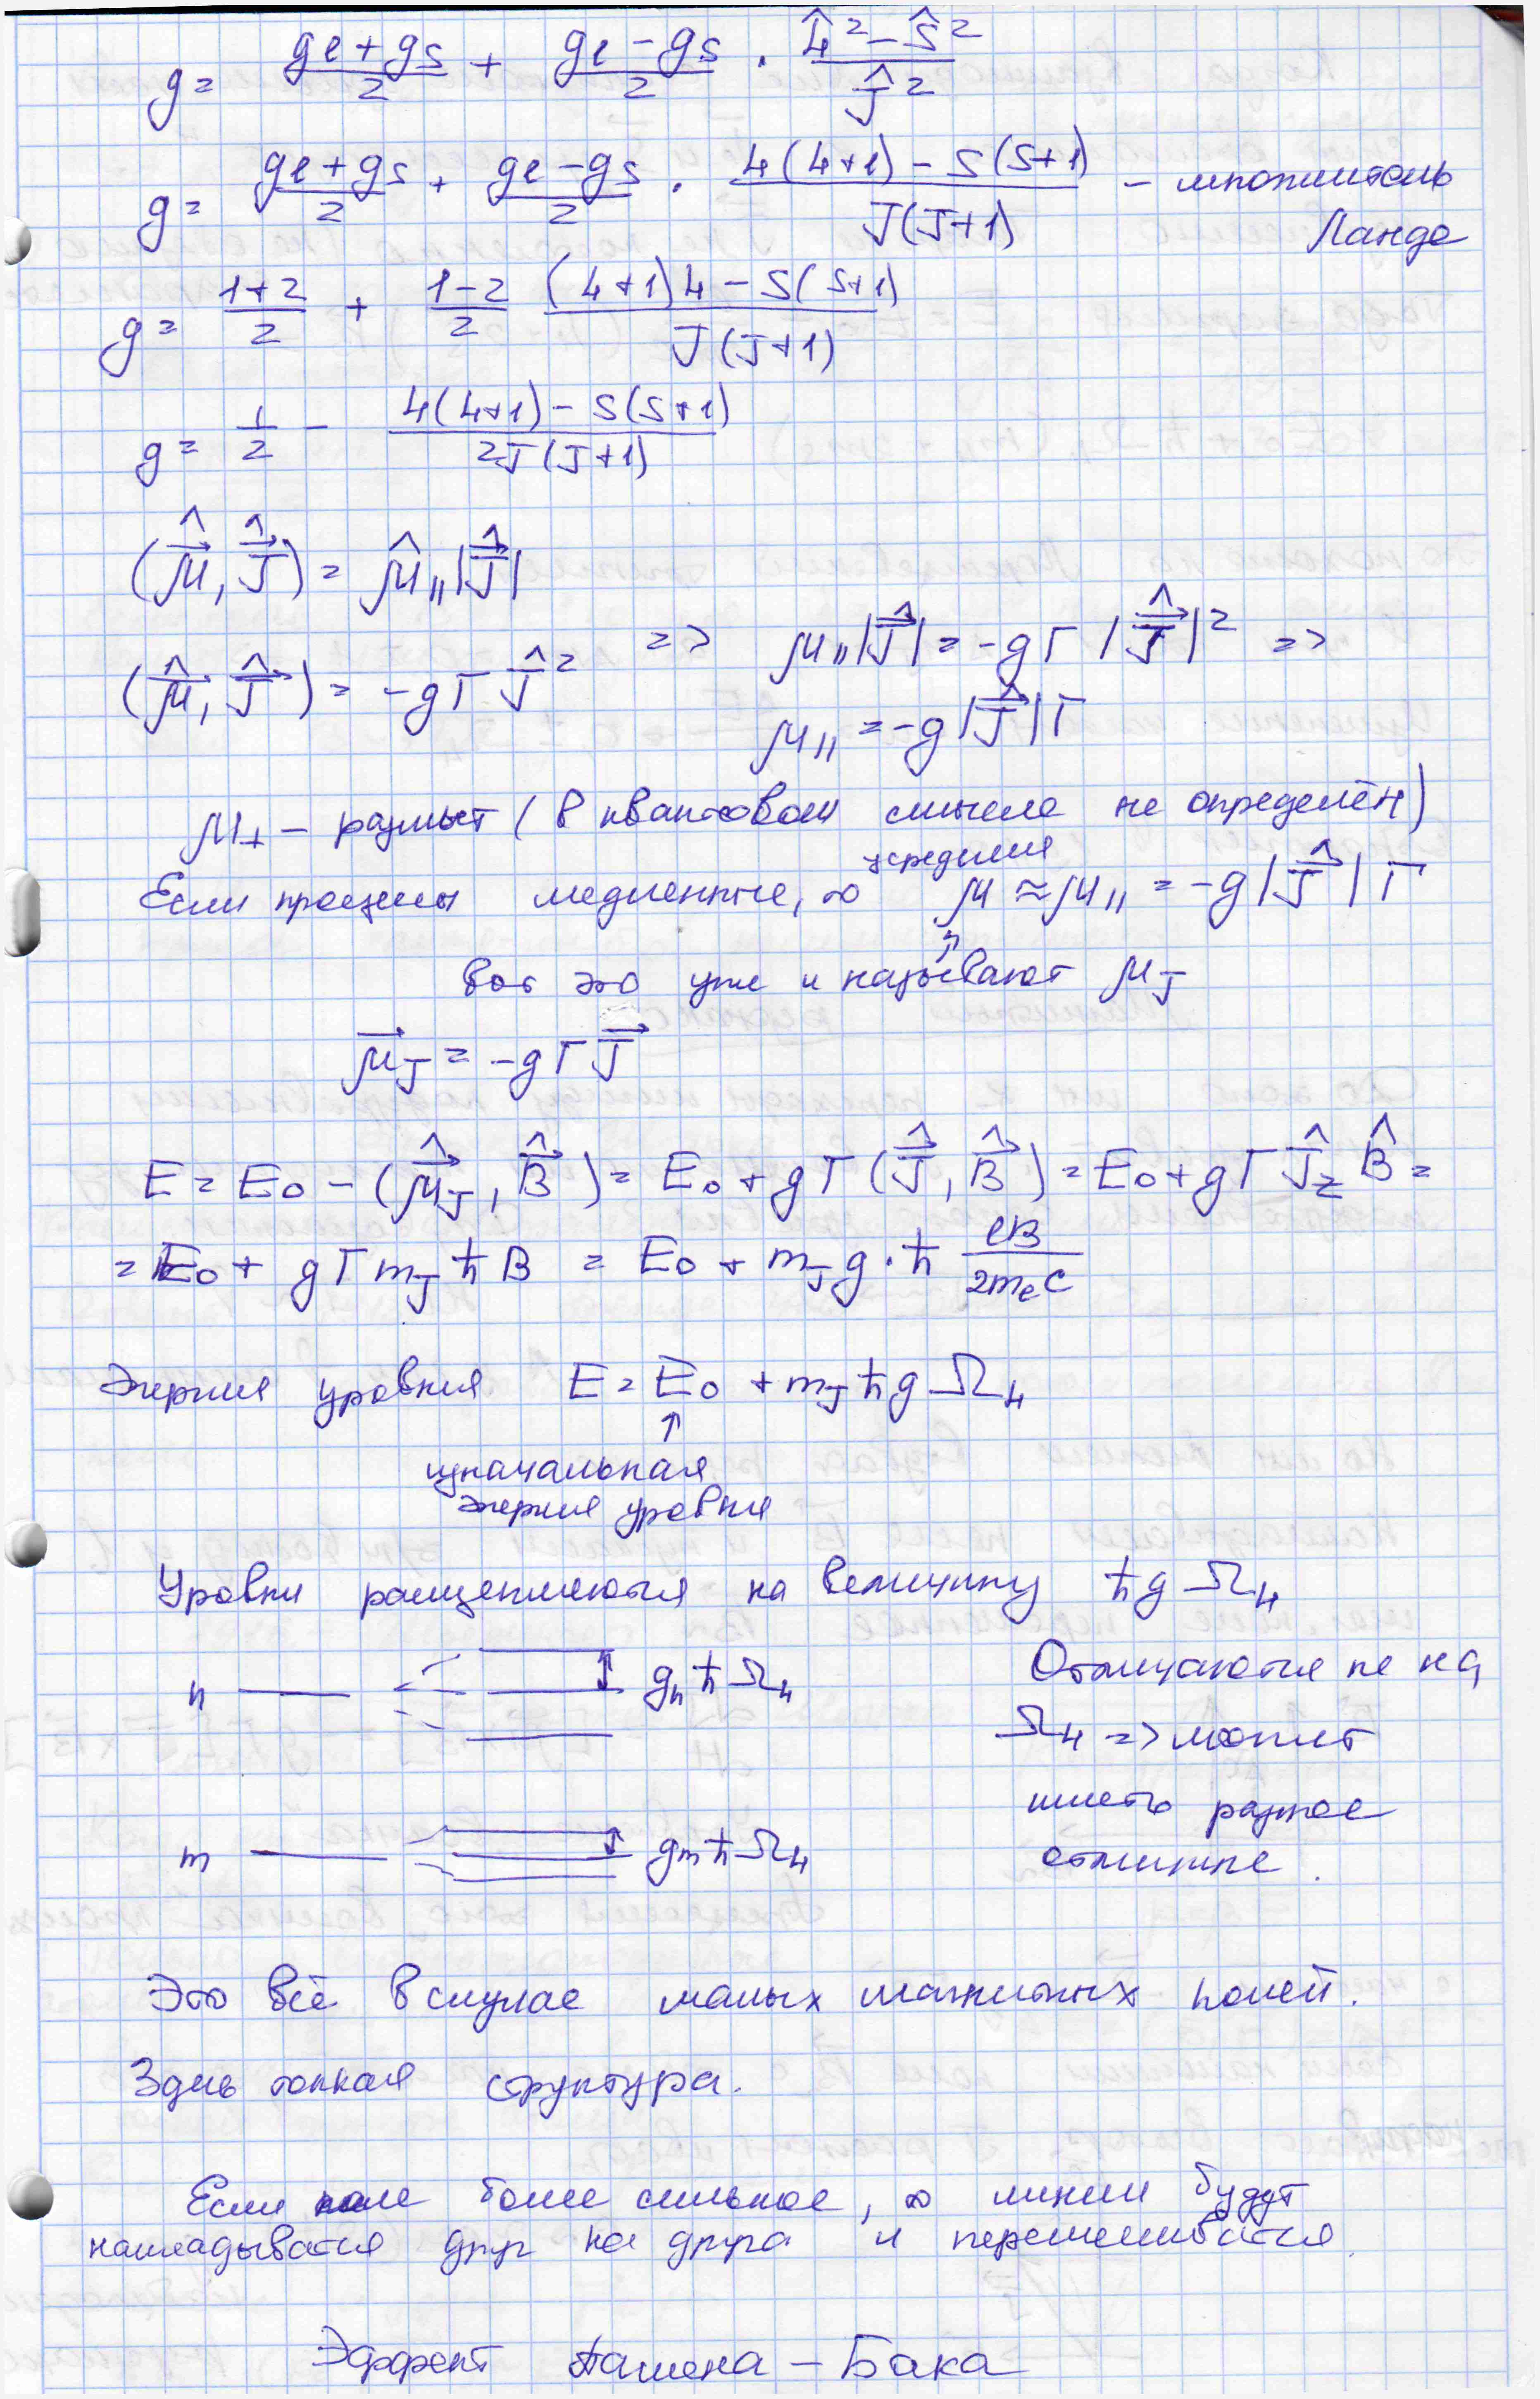
\includegraphics[max size={\textwidth}{0.995\textheight}]{jpg/10.jpg}%
\newpage%
%
%
\phantomsection
\addcontentsline{toc}{subsection}{Магнитный резонанс}%
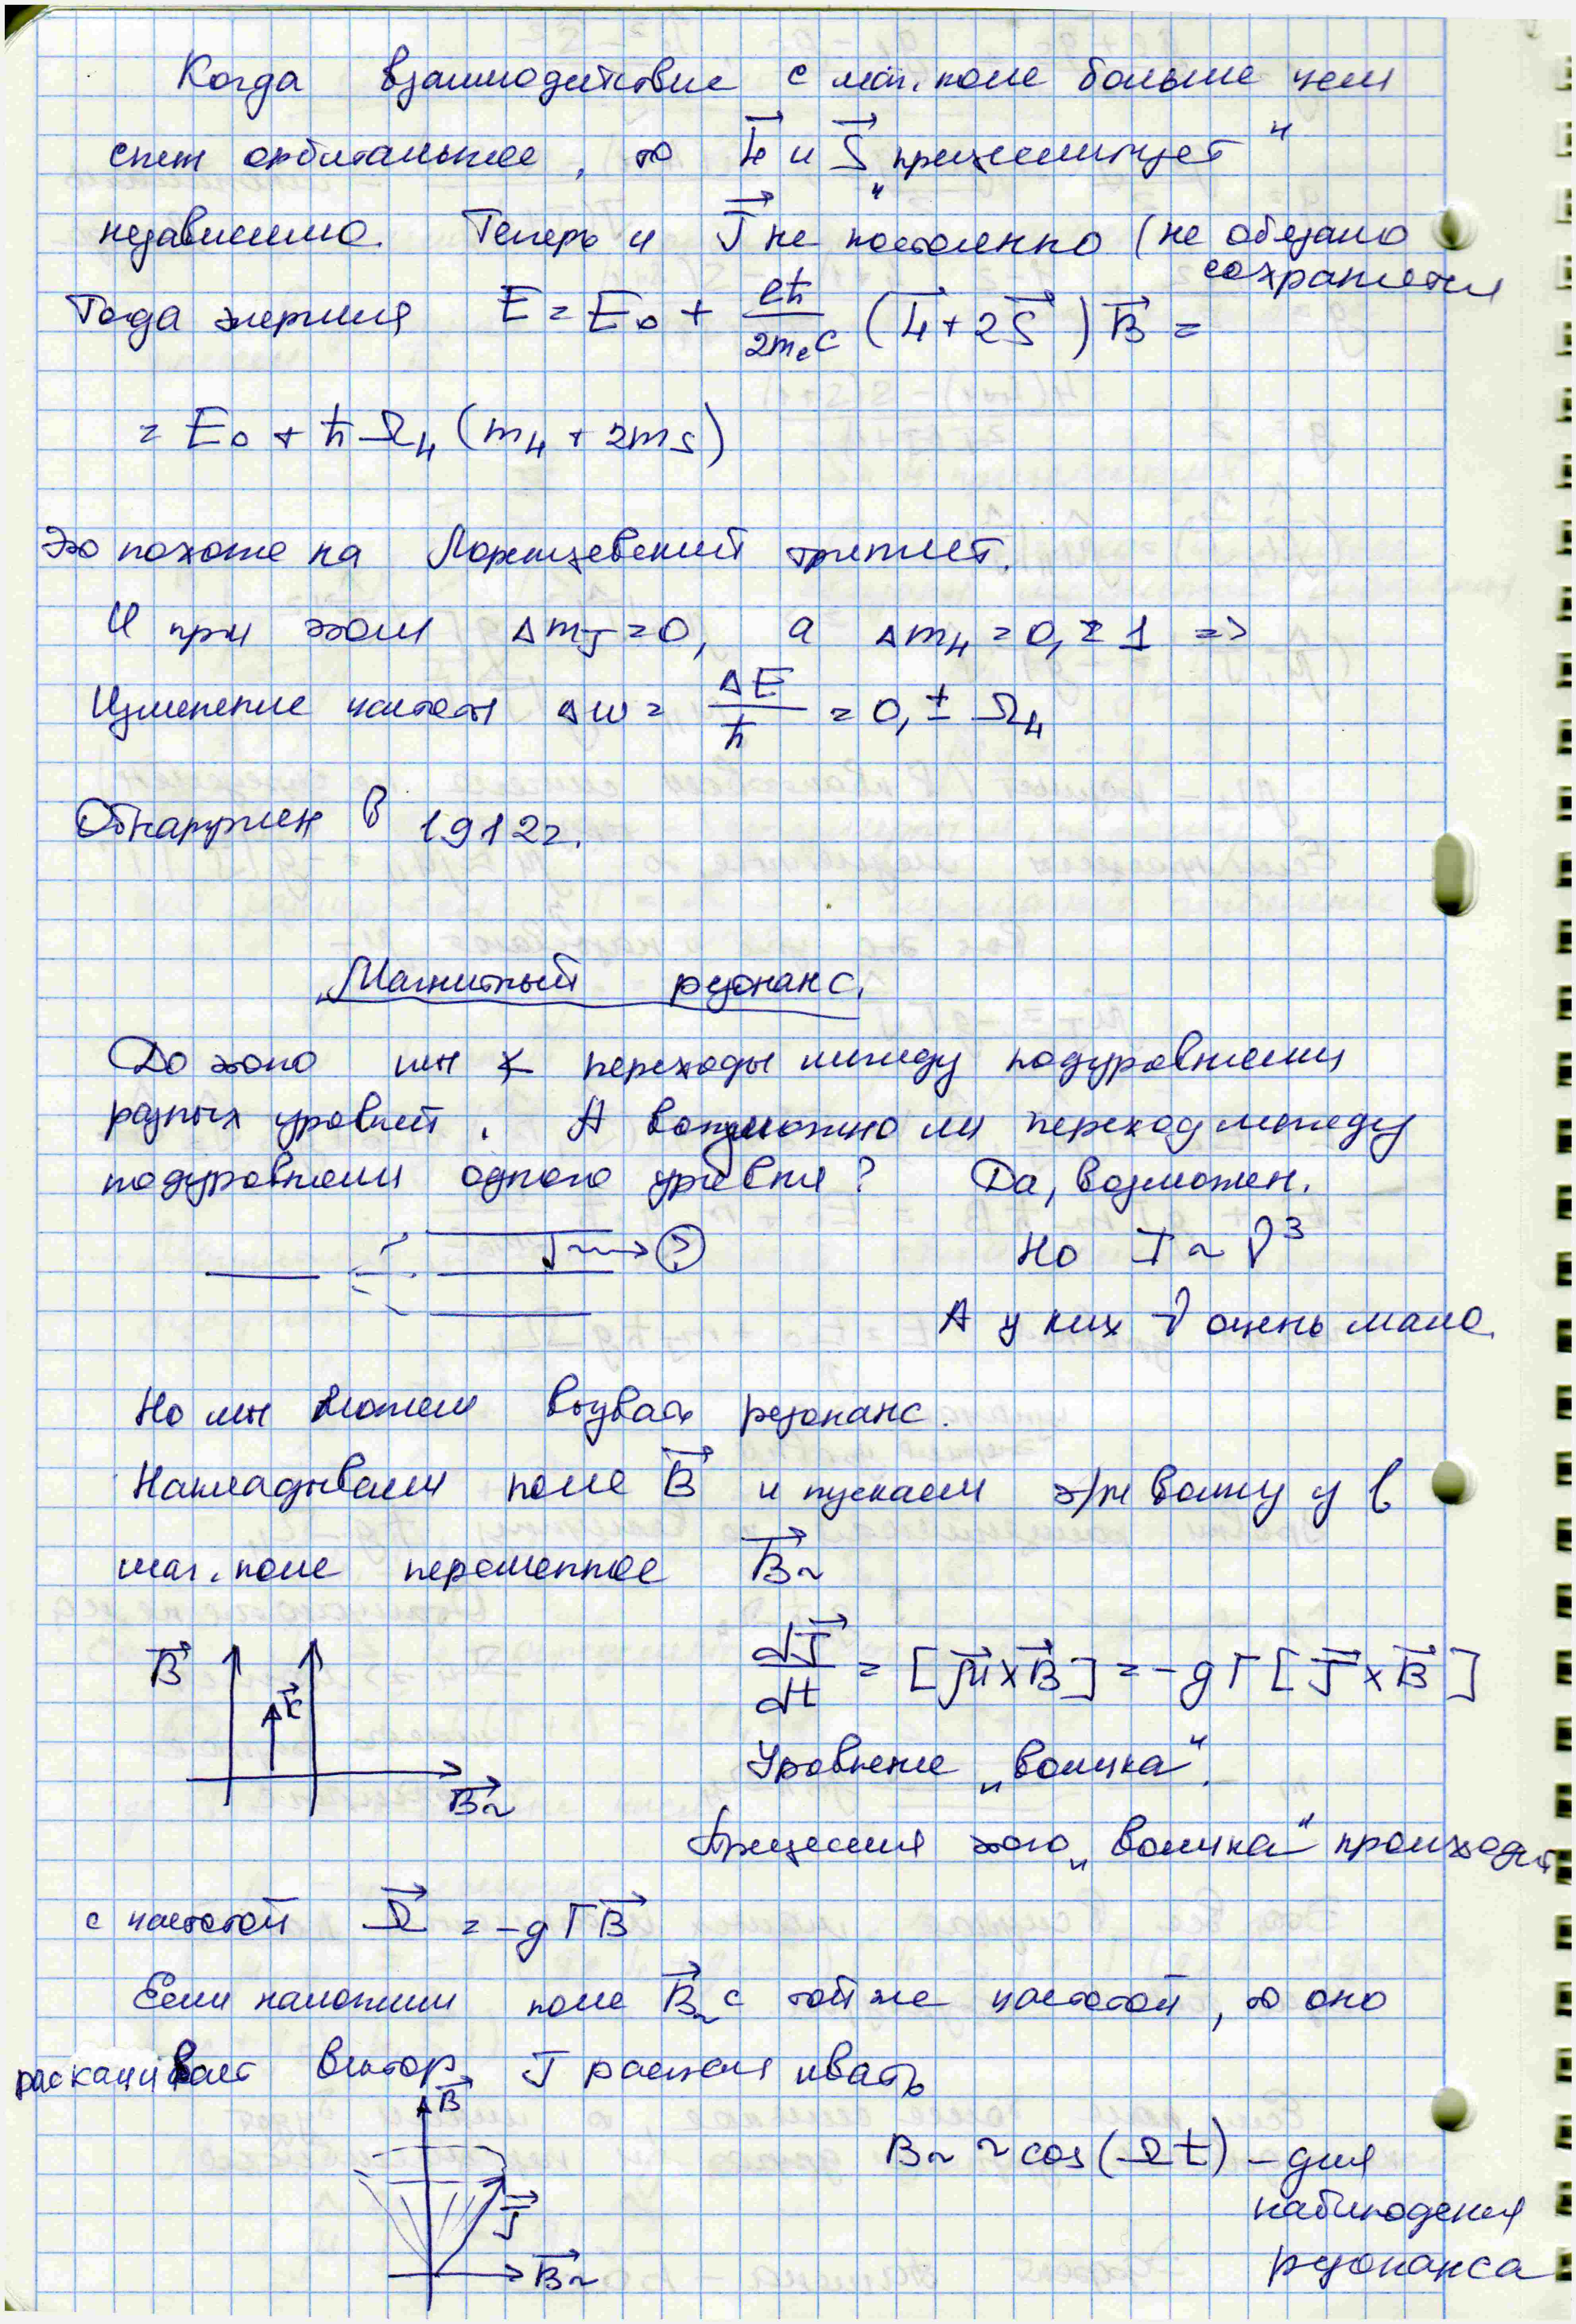
\includegraphics[max size={\textwidth}{0.995\textheight}]{jpg/11.jpg}%
\newpage%
%
%
\phantomsection\addcontentsline{toc}{subsection}{Эффект Штарка}%
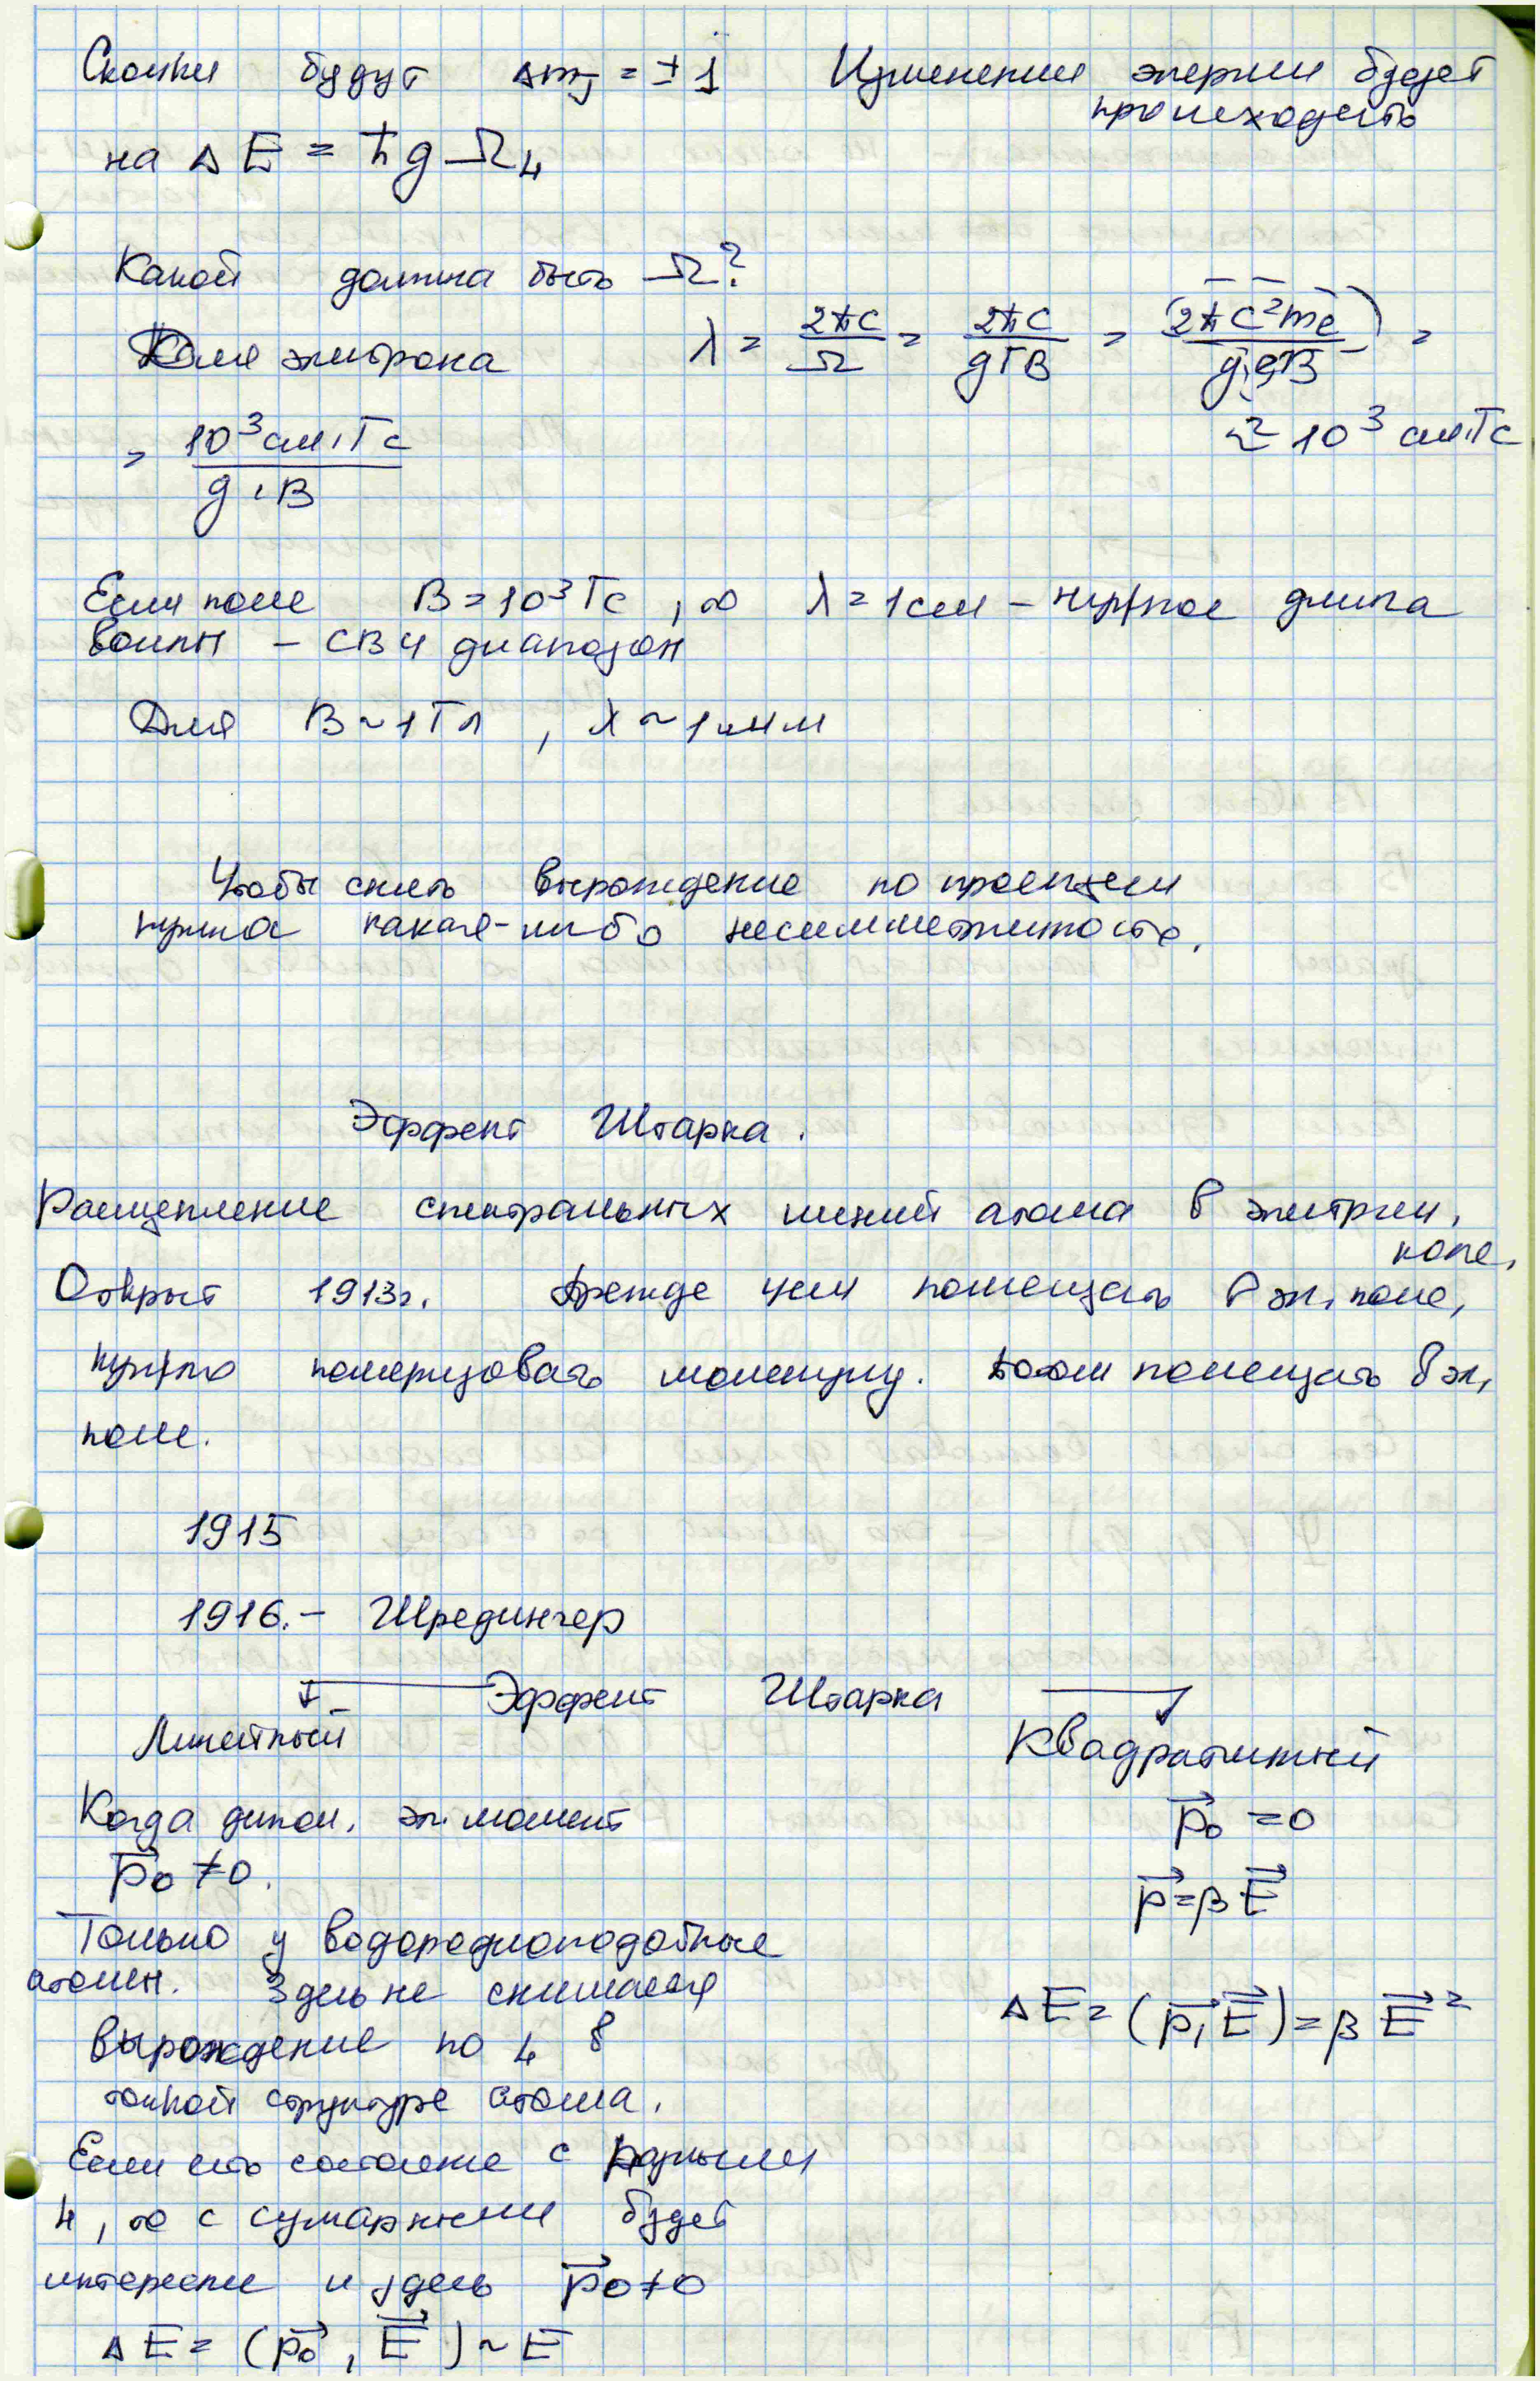
\includegraphics[max size={\textwidth}{0.995\textheight}]{jpg/12.jpg}%
\newpage%
%
%

\phantomsection\addcontentsline{toc}{section}{Многоэлектронные квантовые системы}%
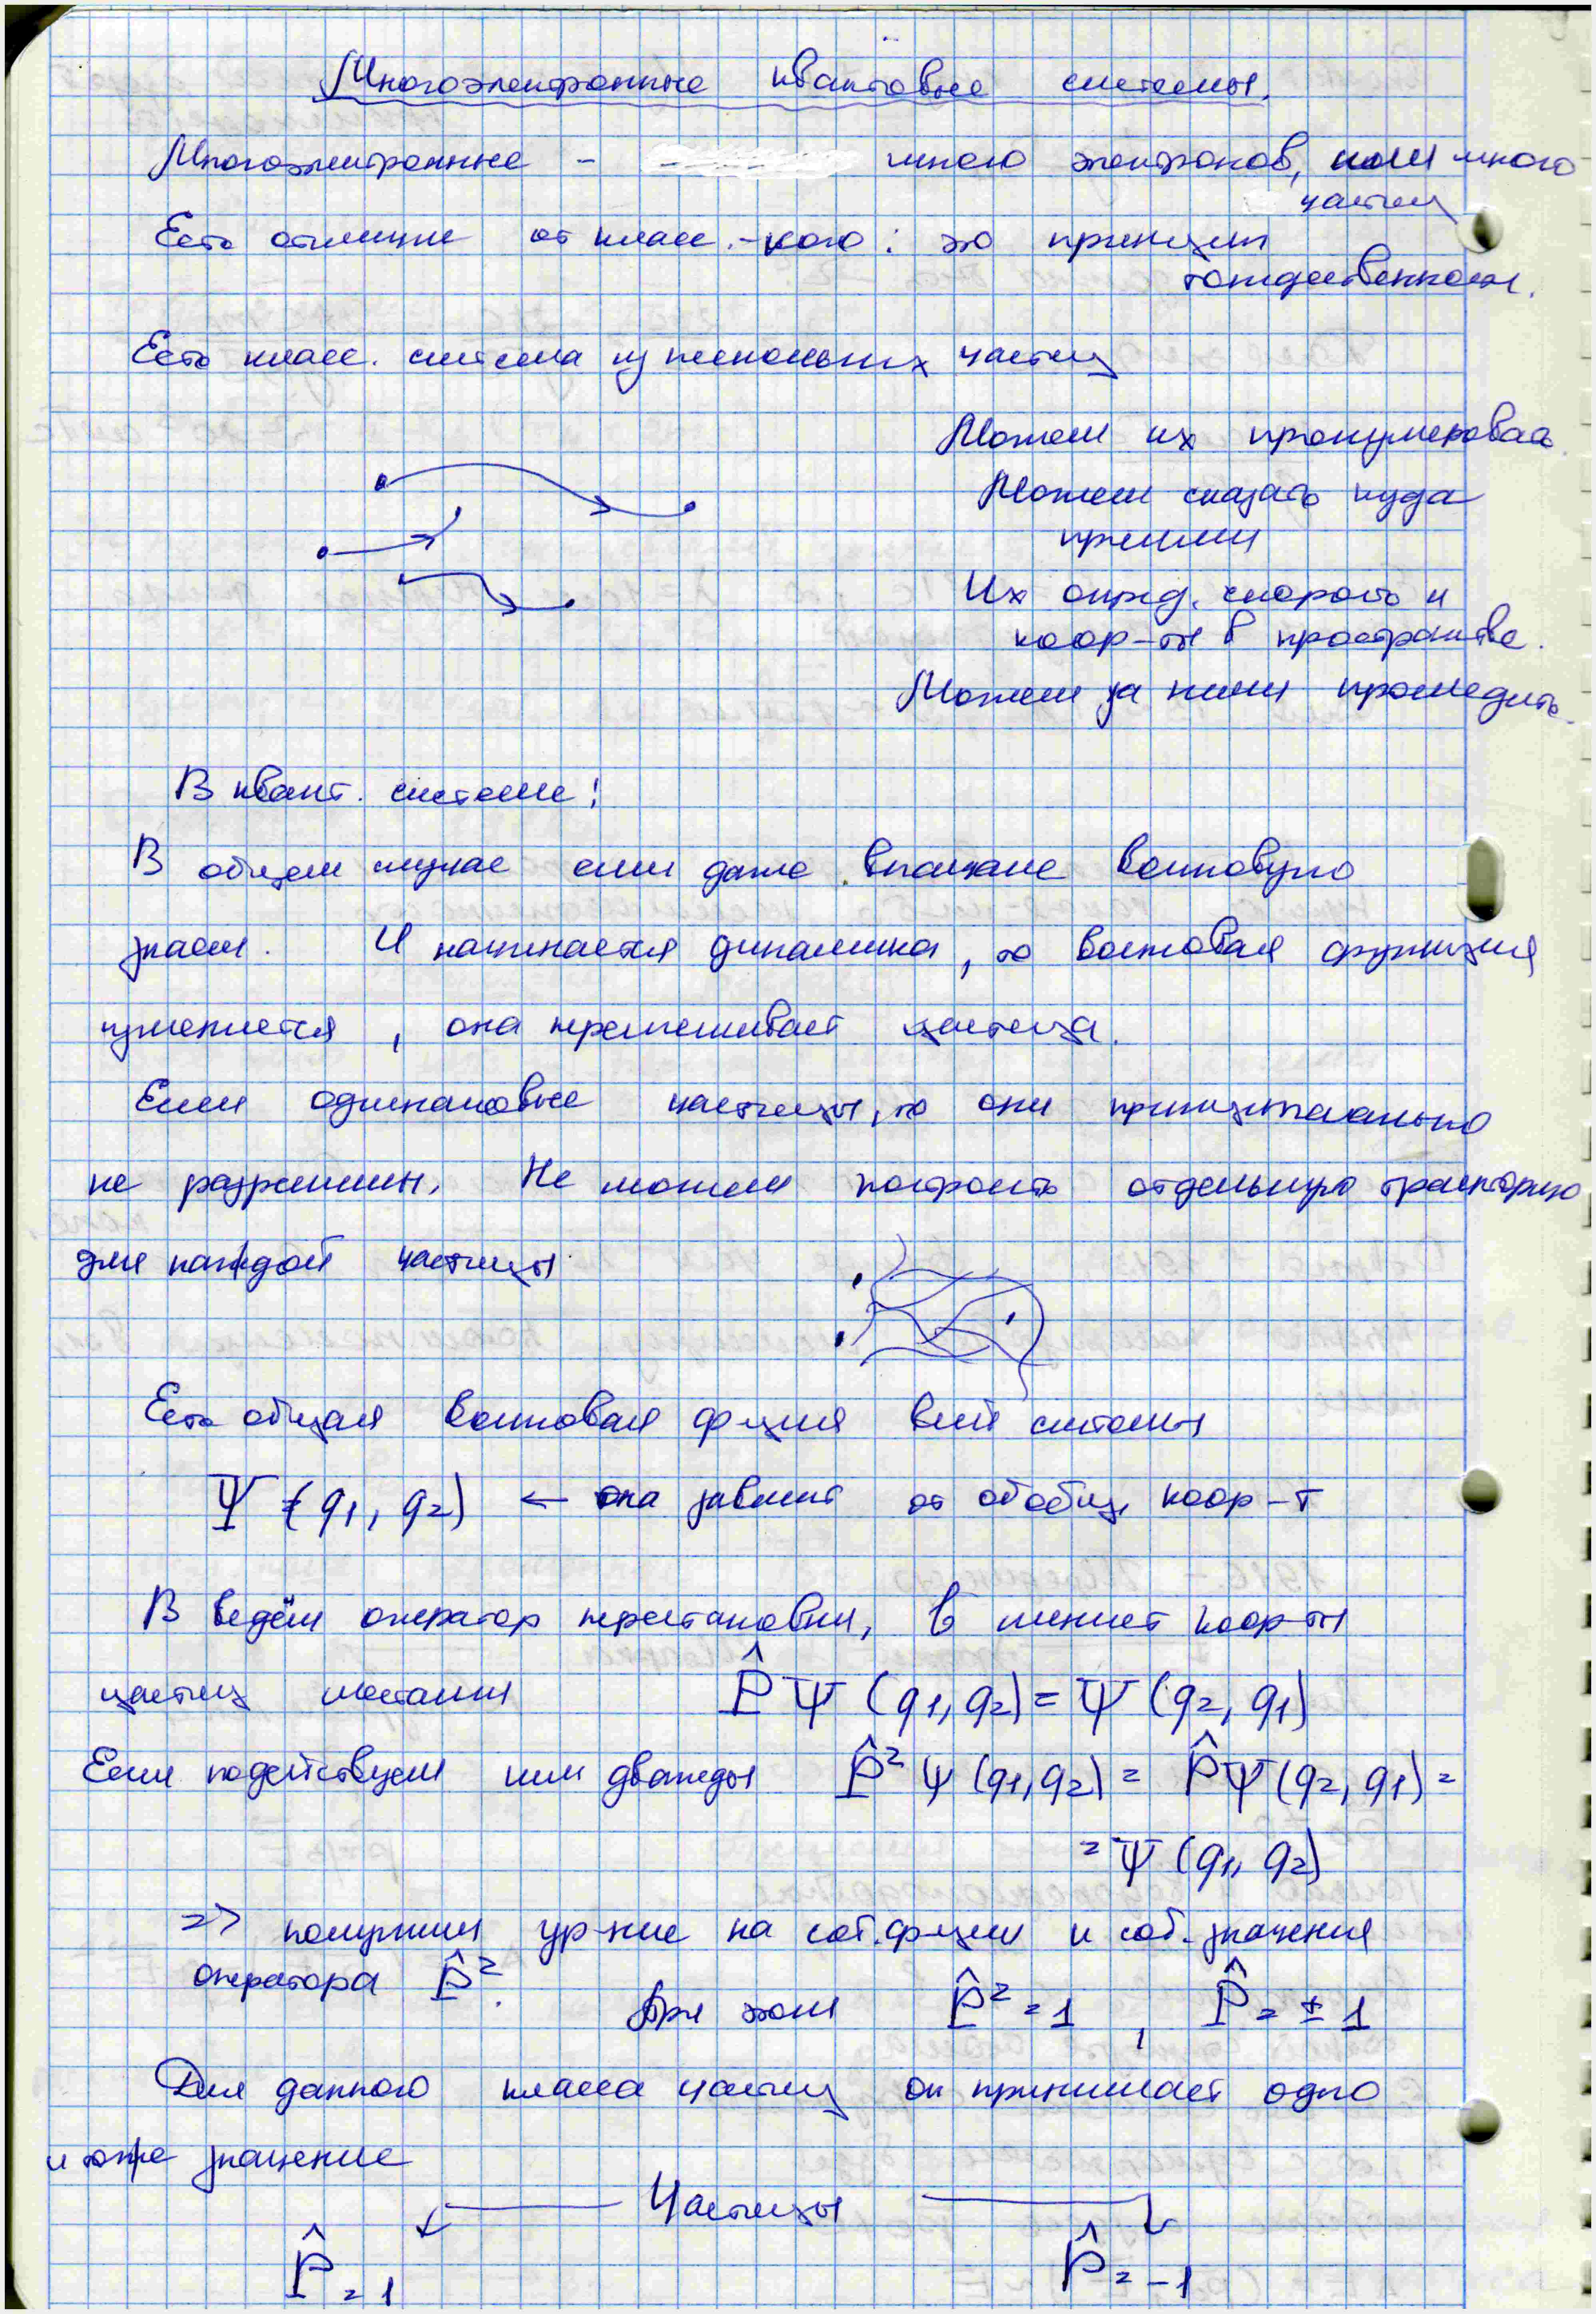
\includegraphics[max size={\textwidth}{0.995\textheight}]{jpg/13.jpg}%
\newpage%
%
%
\phantomsection\addcontentsline{toc}{subsection}{Принцип запрета Паули}%
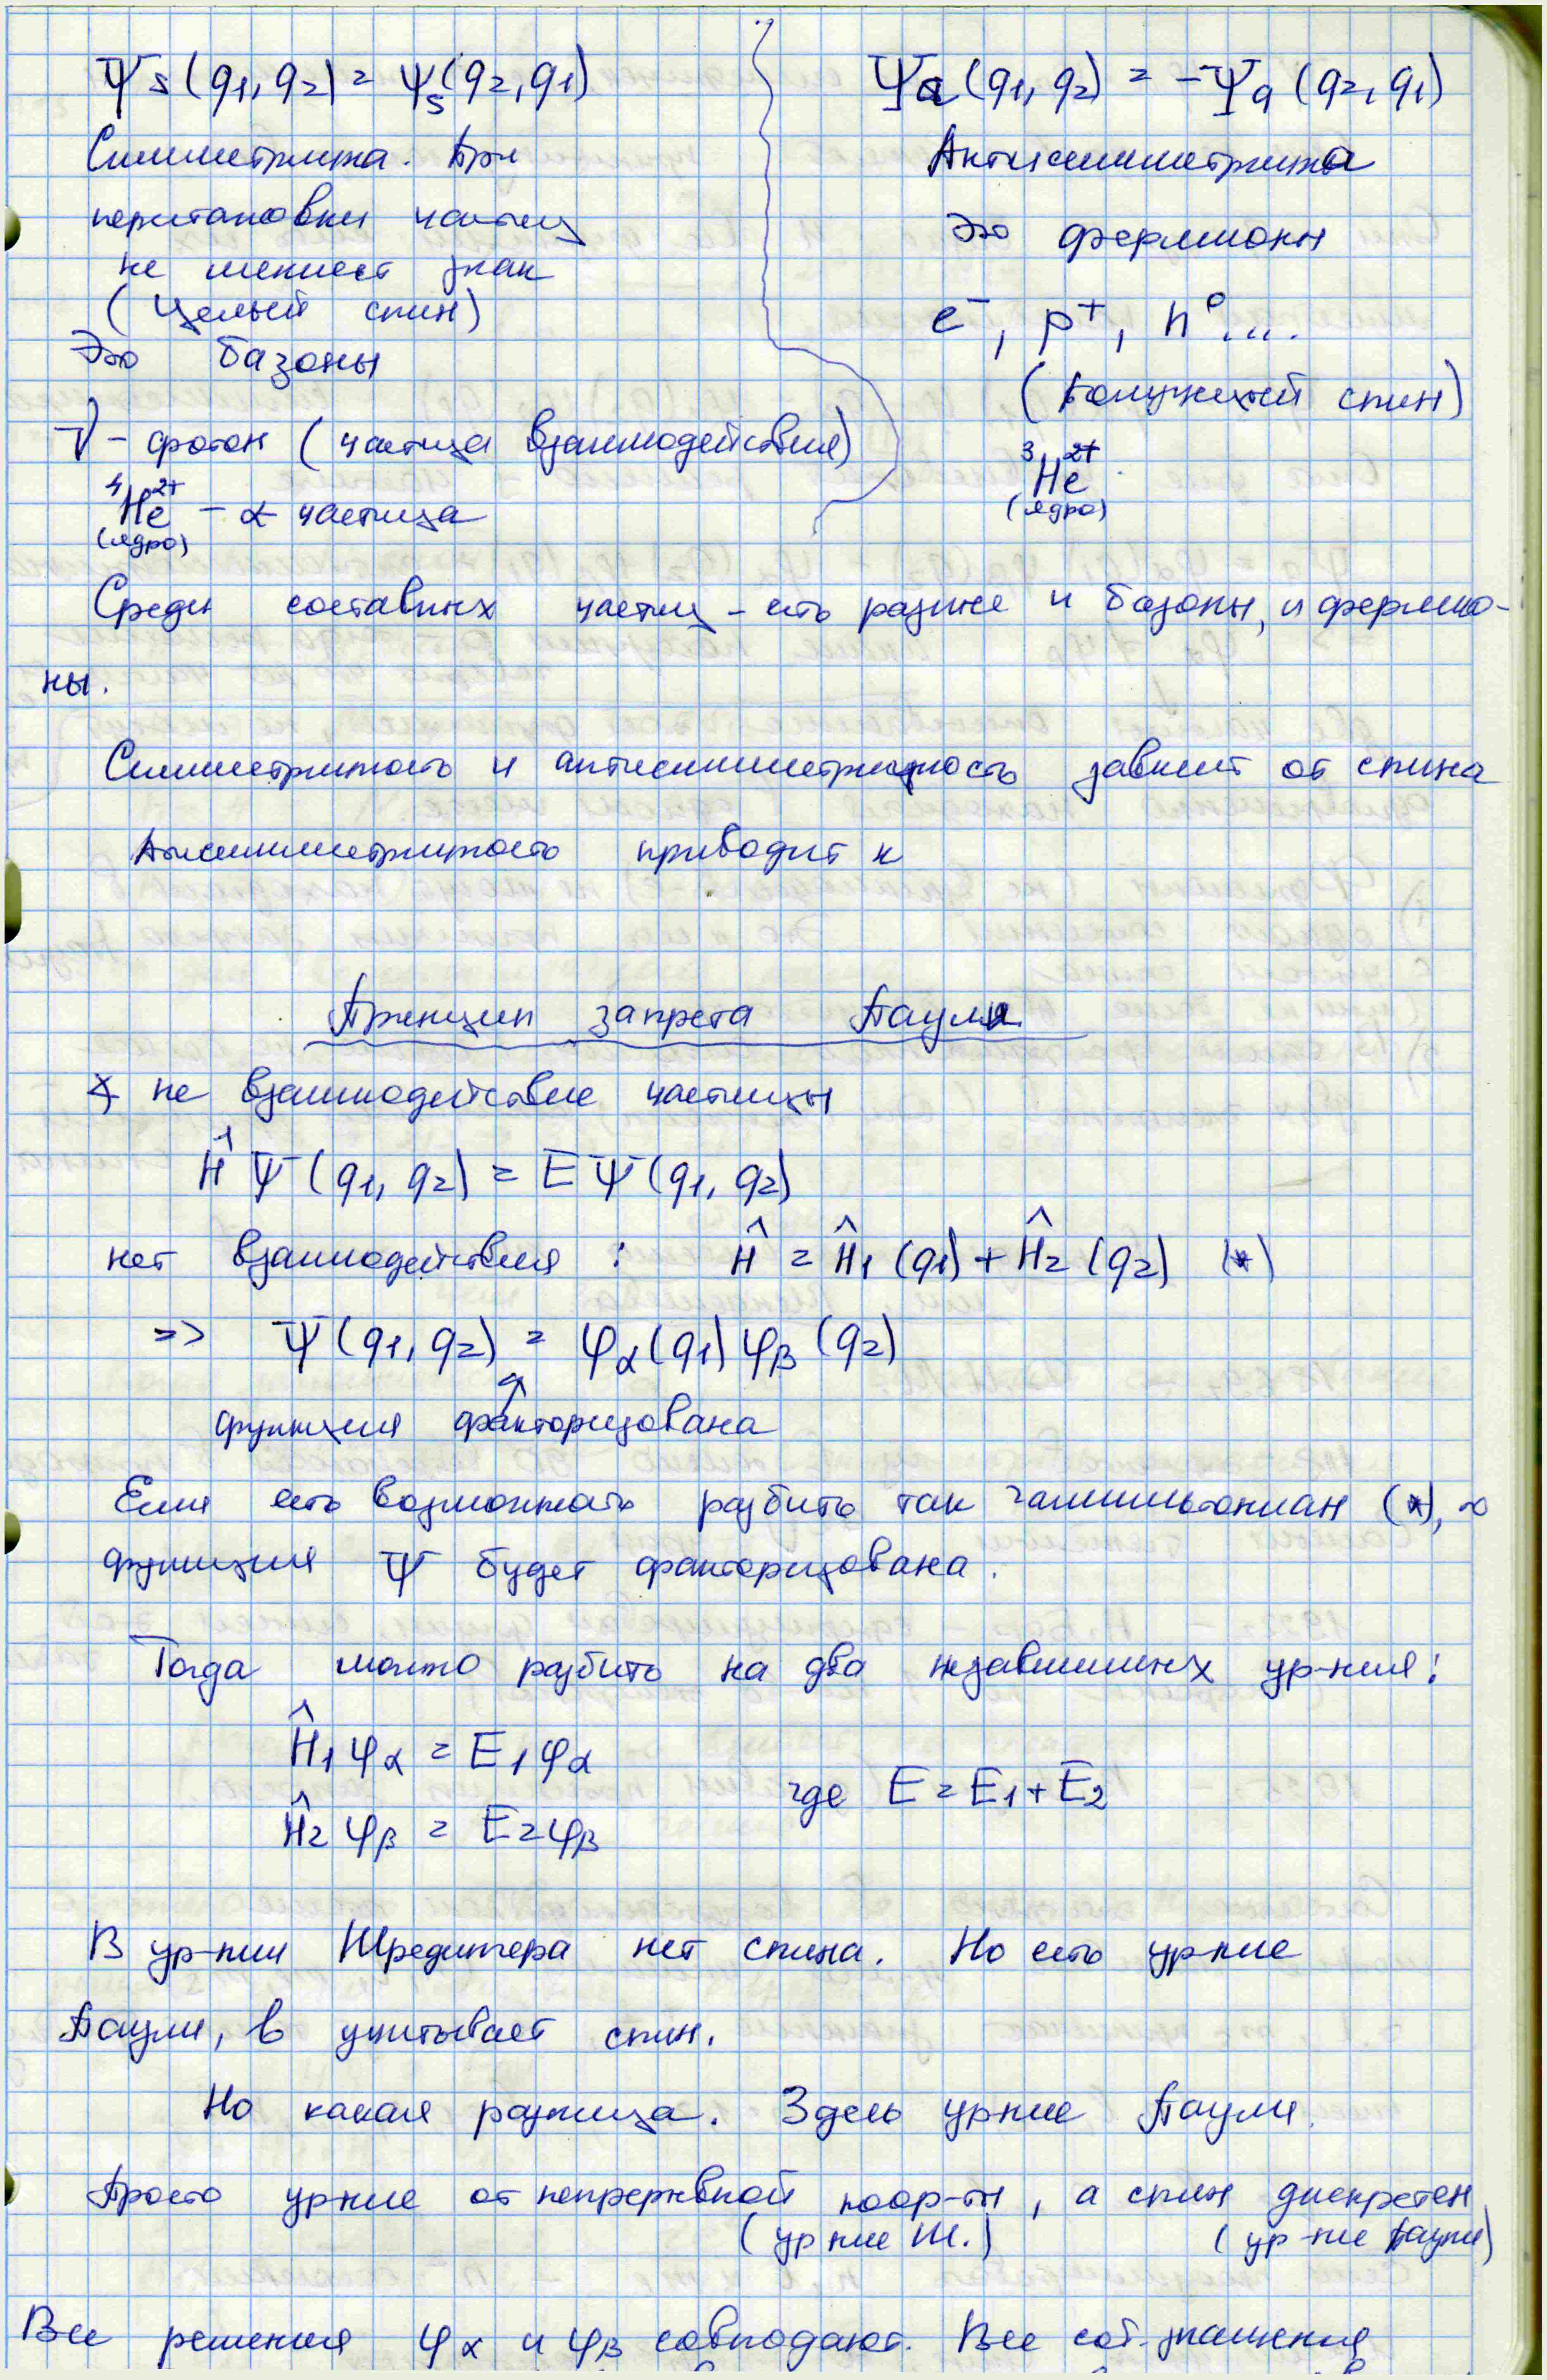
\includegraphics[max size={\textwidth}{0.995\textheight}]{jpg/14.jpg}%
\newpage%
%
%
\phantomsection\addcontentsline{toc}{subsection}{Периодическая система Менделеева}%
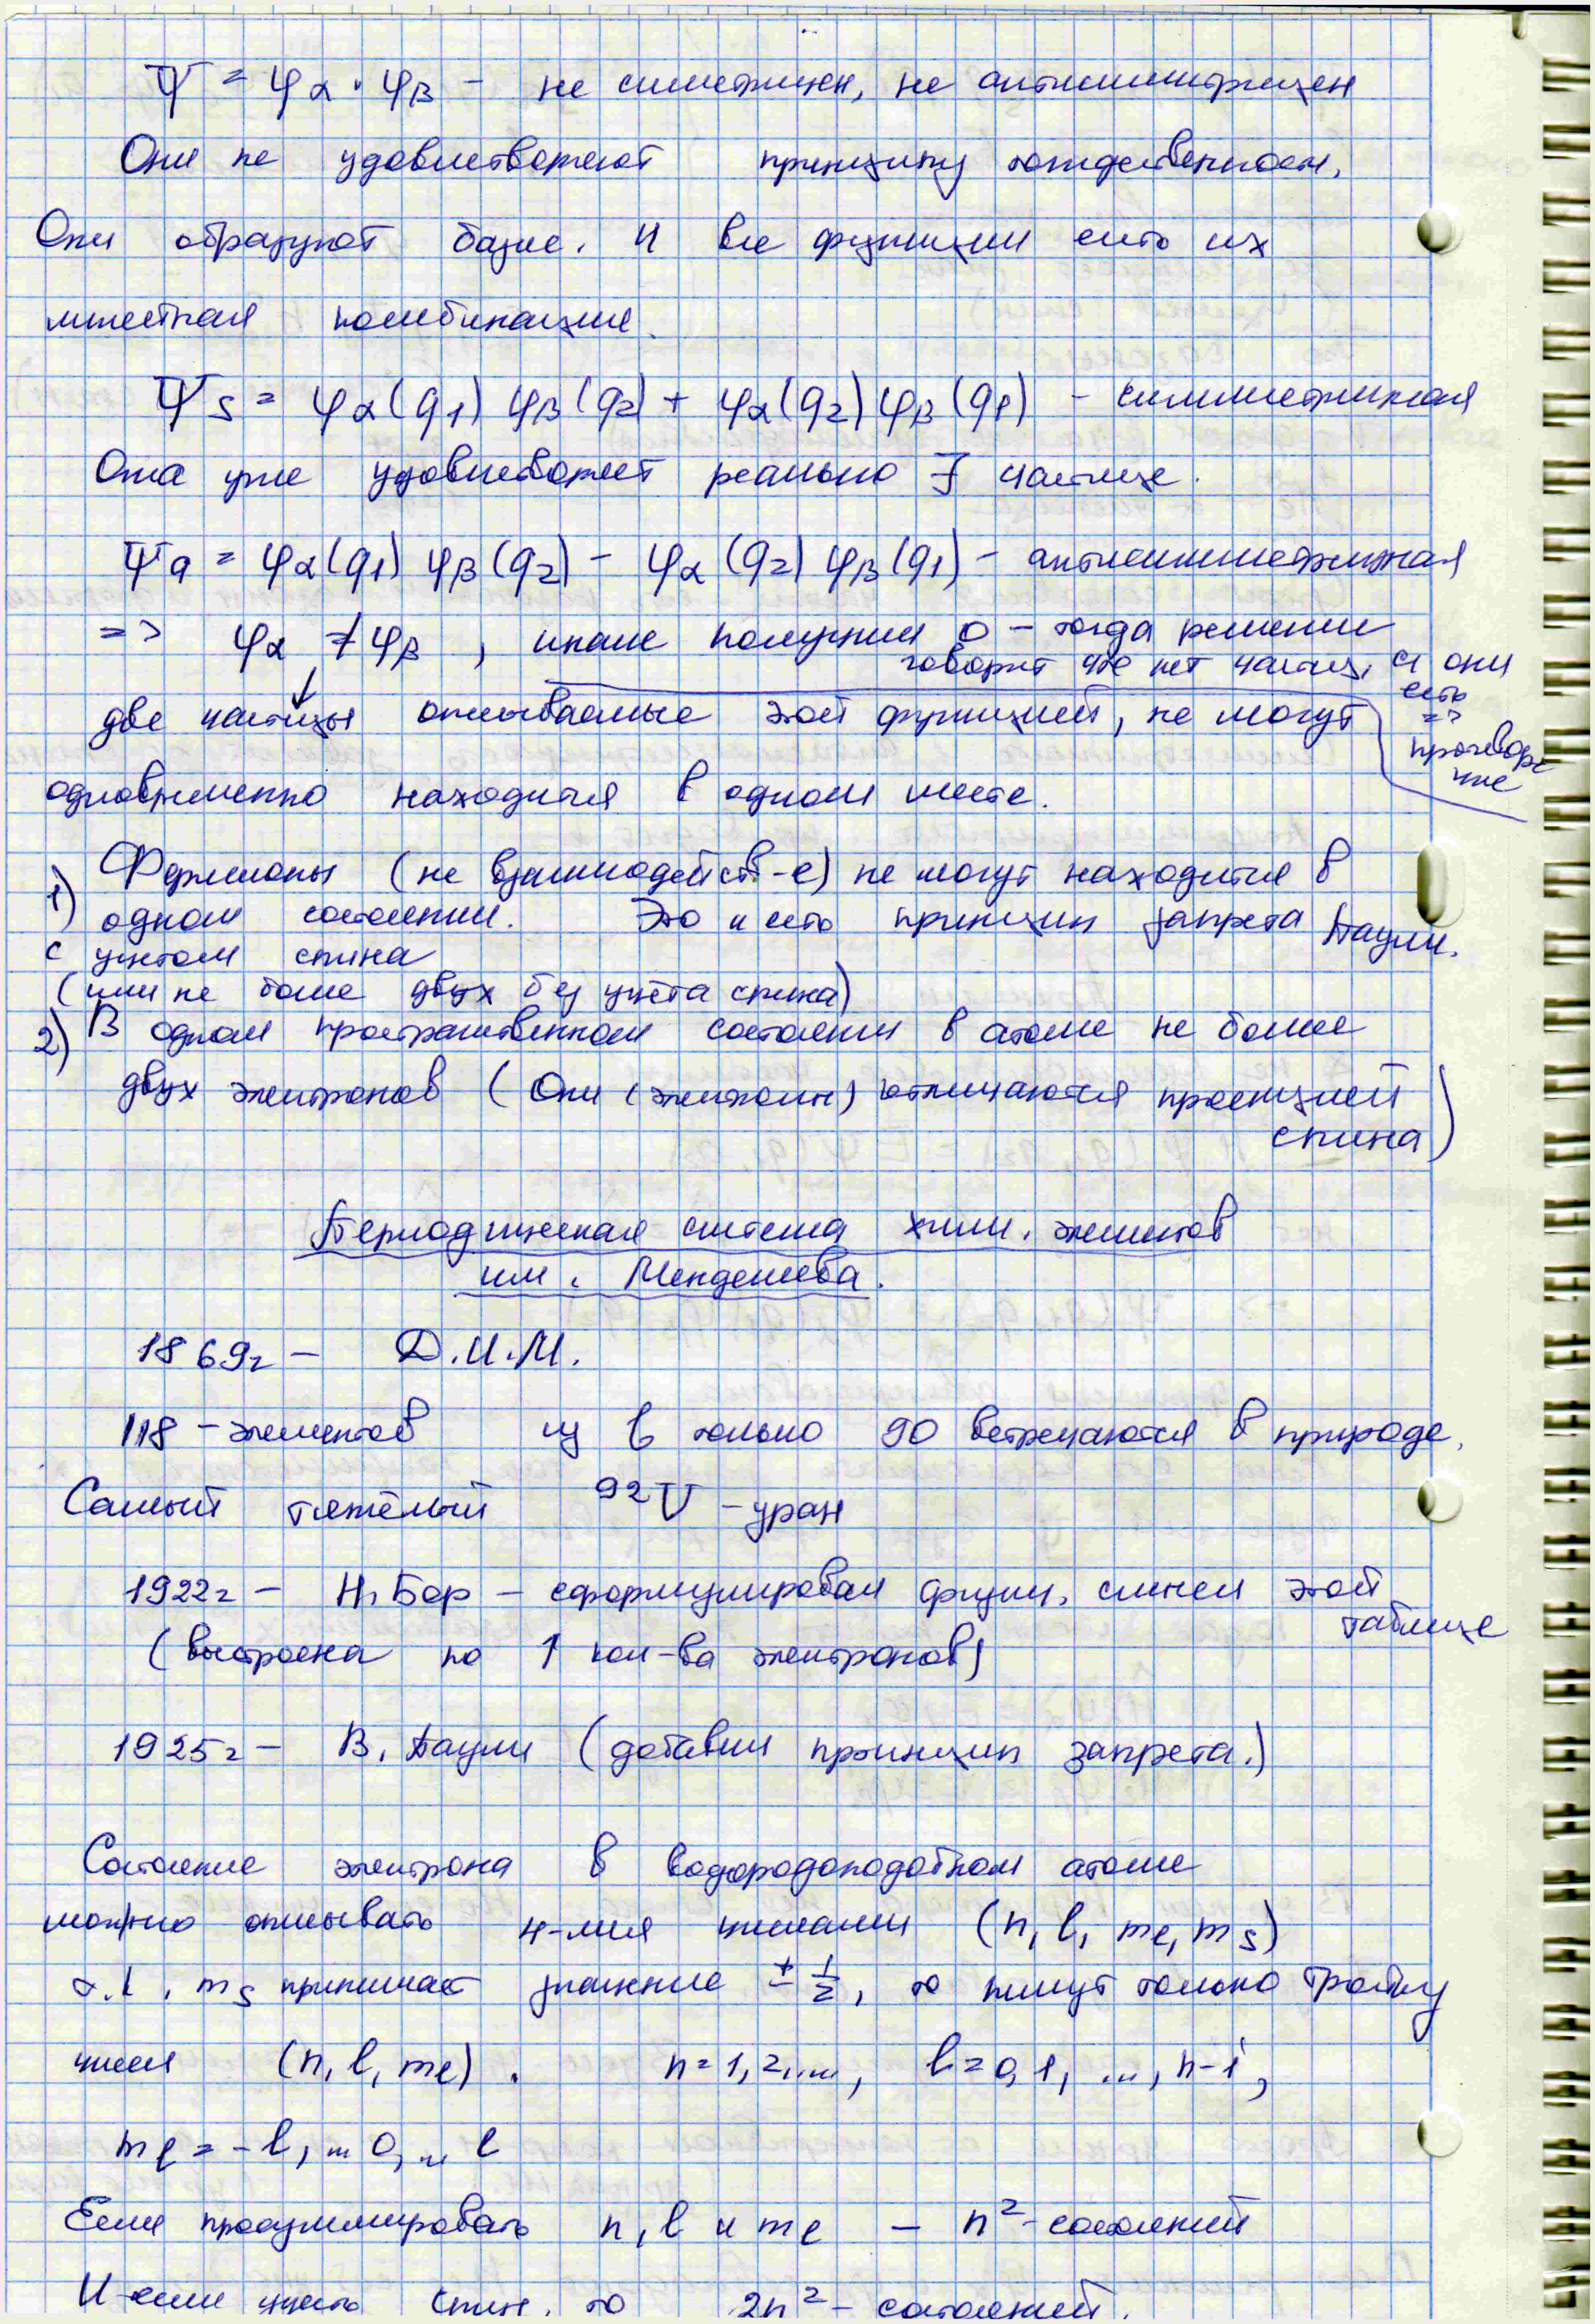
\includegraphics[max size={\textwidth}{0.995\textheight}]{jpg/15.jpg}%
\newpage%
%
%
\phantomsection\addcontentsline{toc}{subsection}{Атом гелия}%
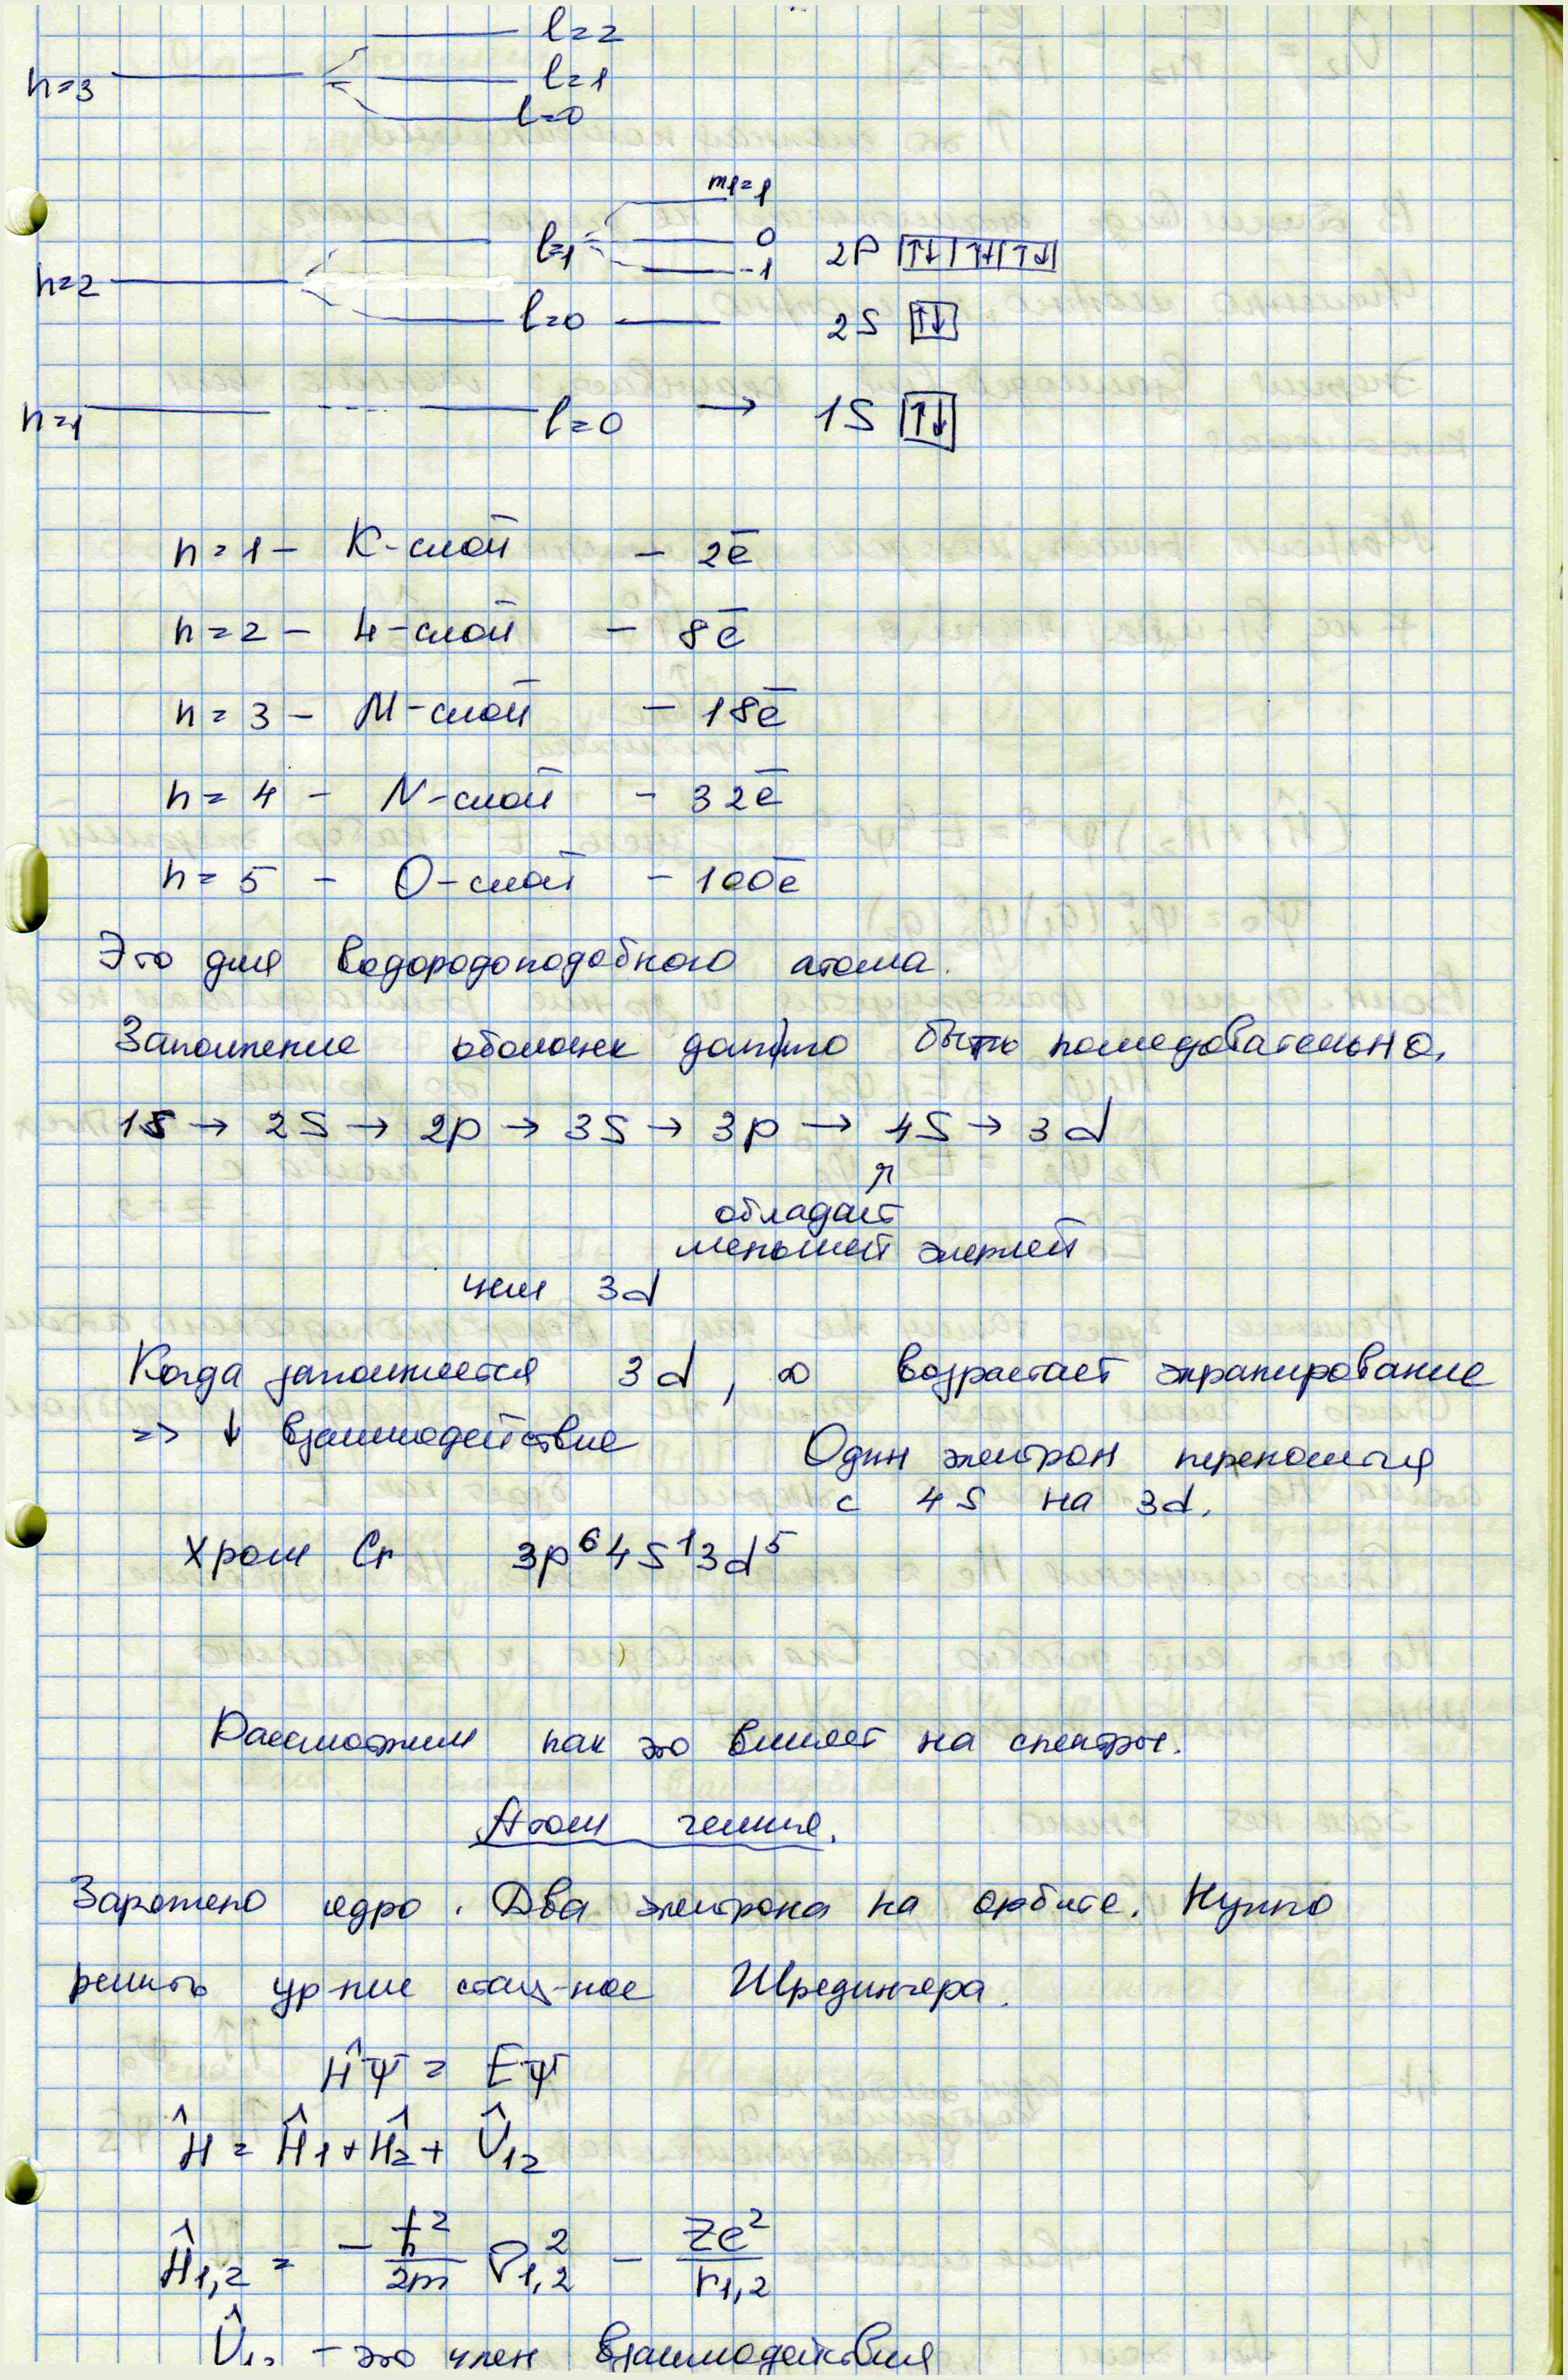
\includegraphics[max size={\textwidth}{0.995\textheight}]{jpg/16.jpg}%
\newpage%
%
%
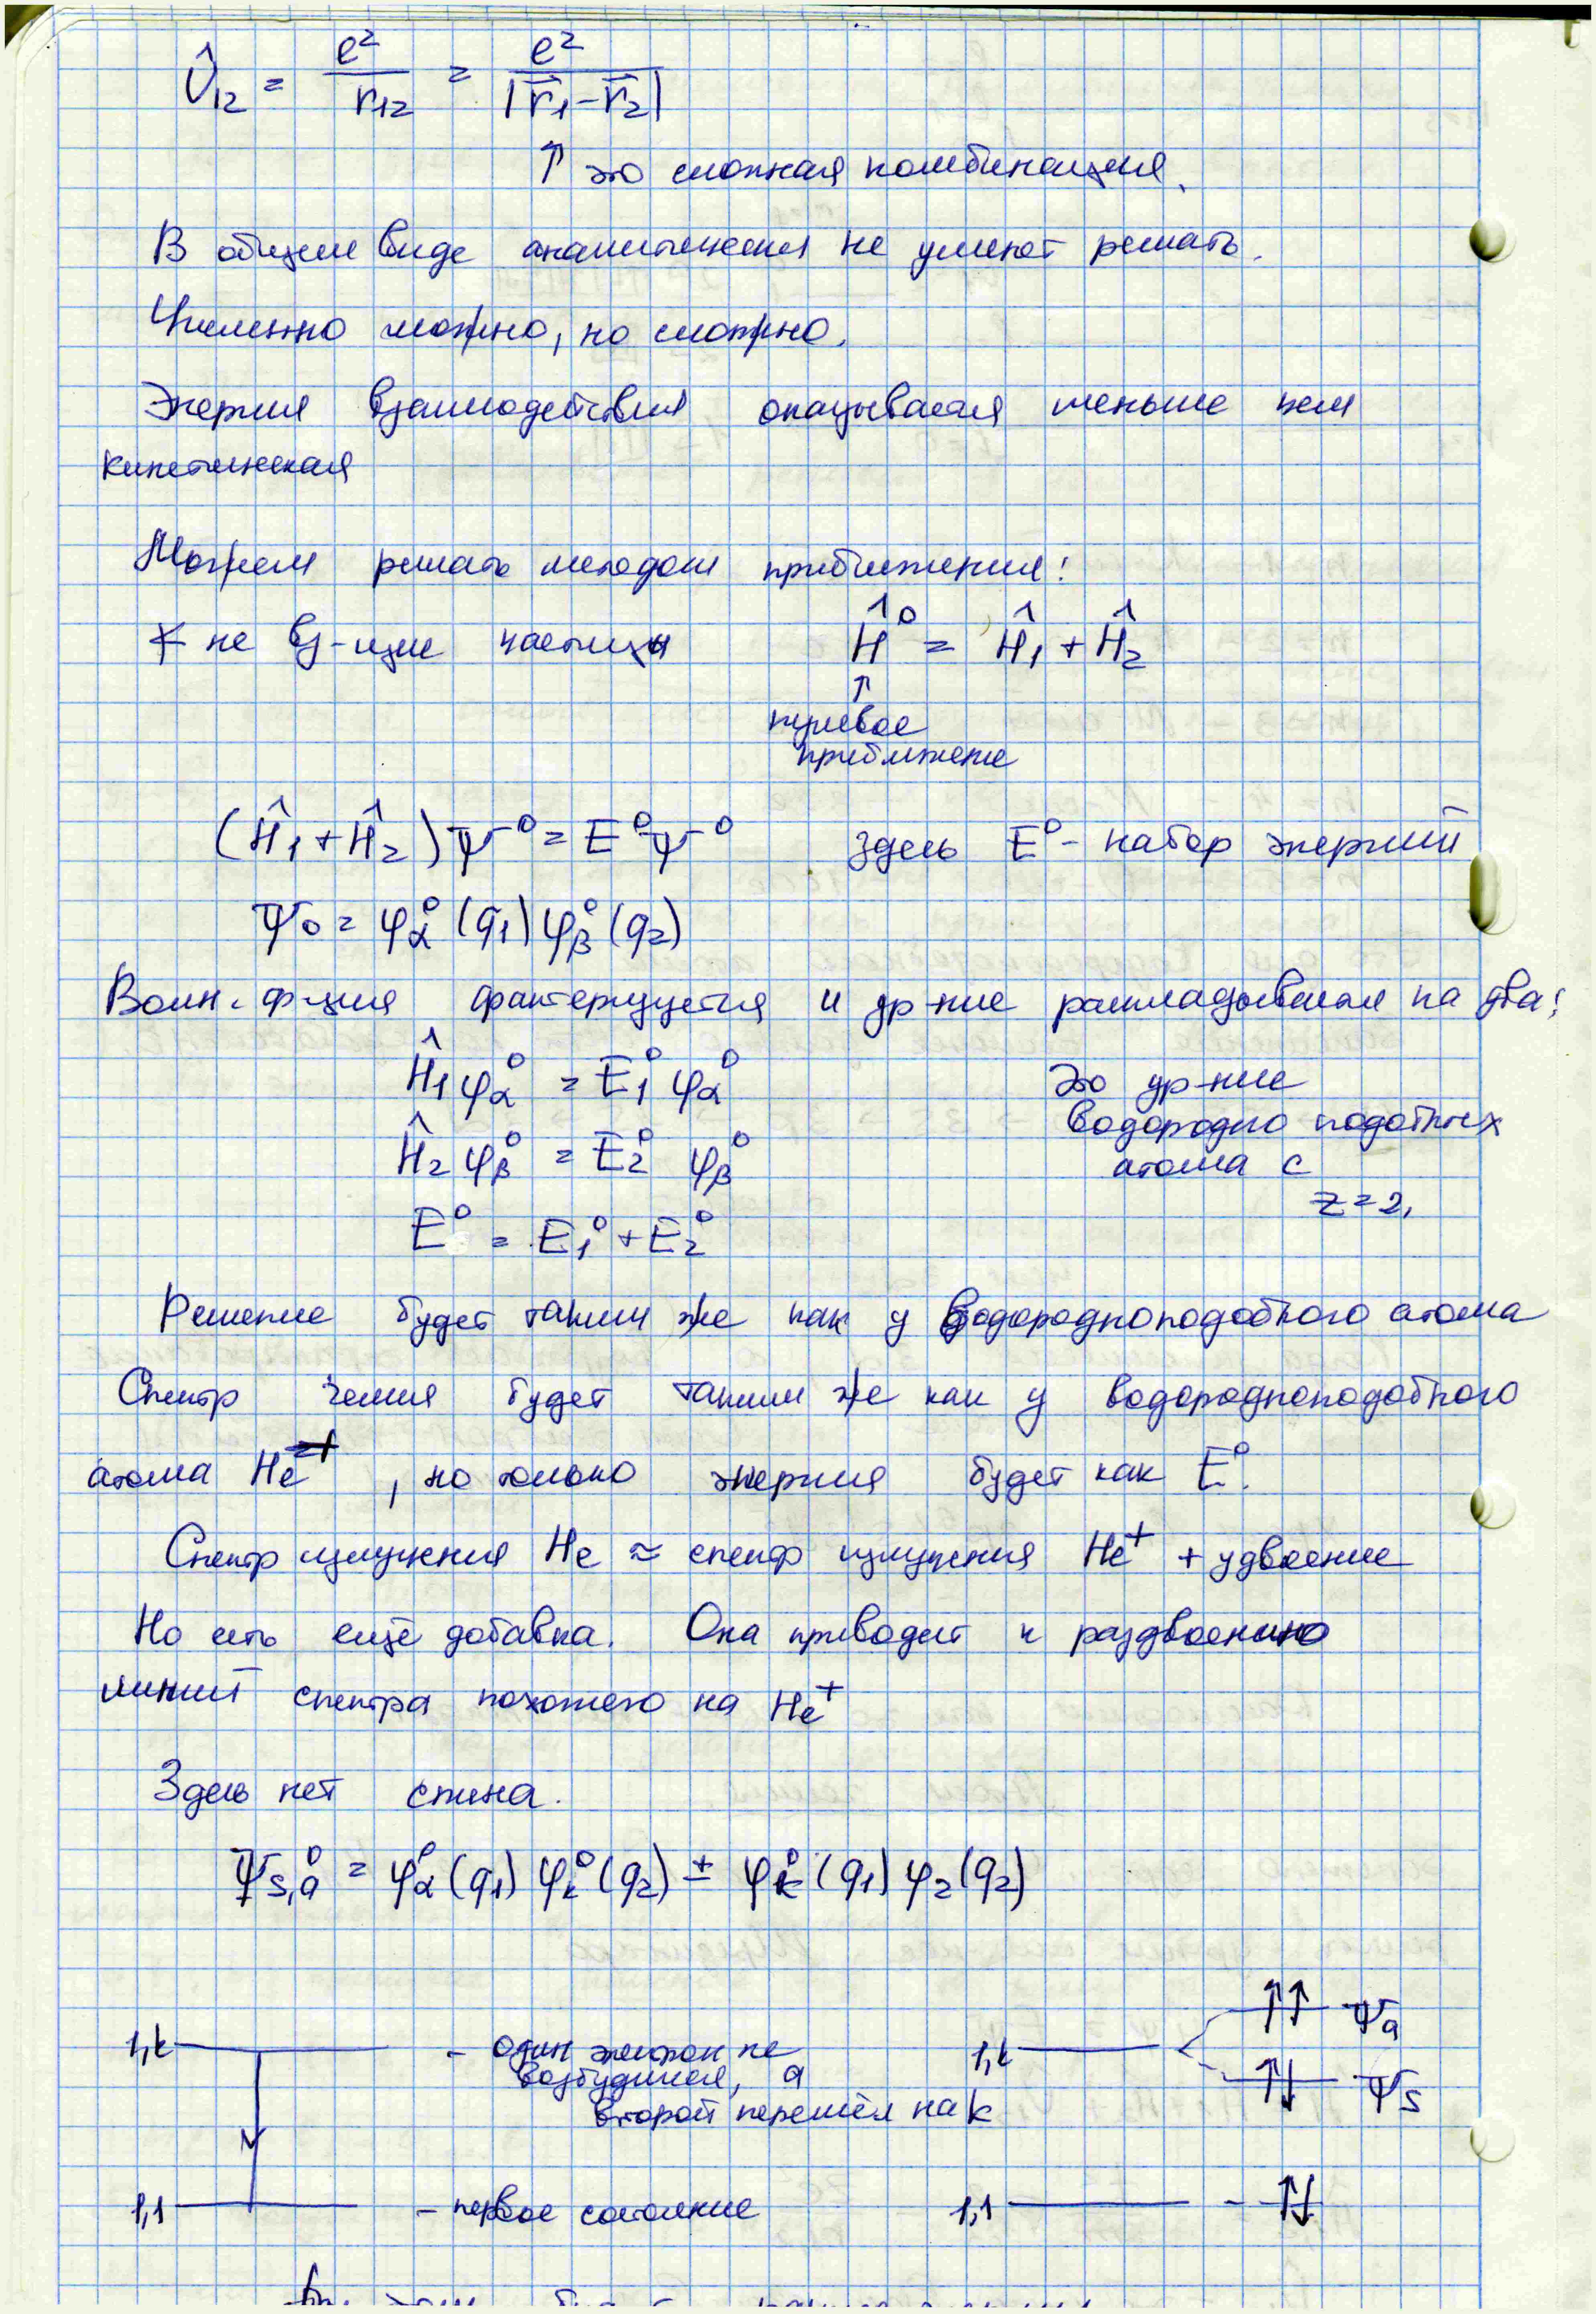
\includegraphics[max size={\textwidth}{0.995\textheight}]{jpg/17.jpg}%
\newpage%
%
%
\phantomsection\addcontentsline{toc}{subsection}{Химическая связь. Молекула водорода}%
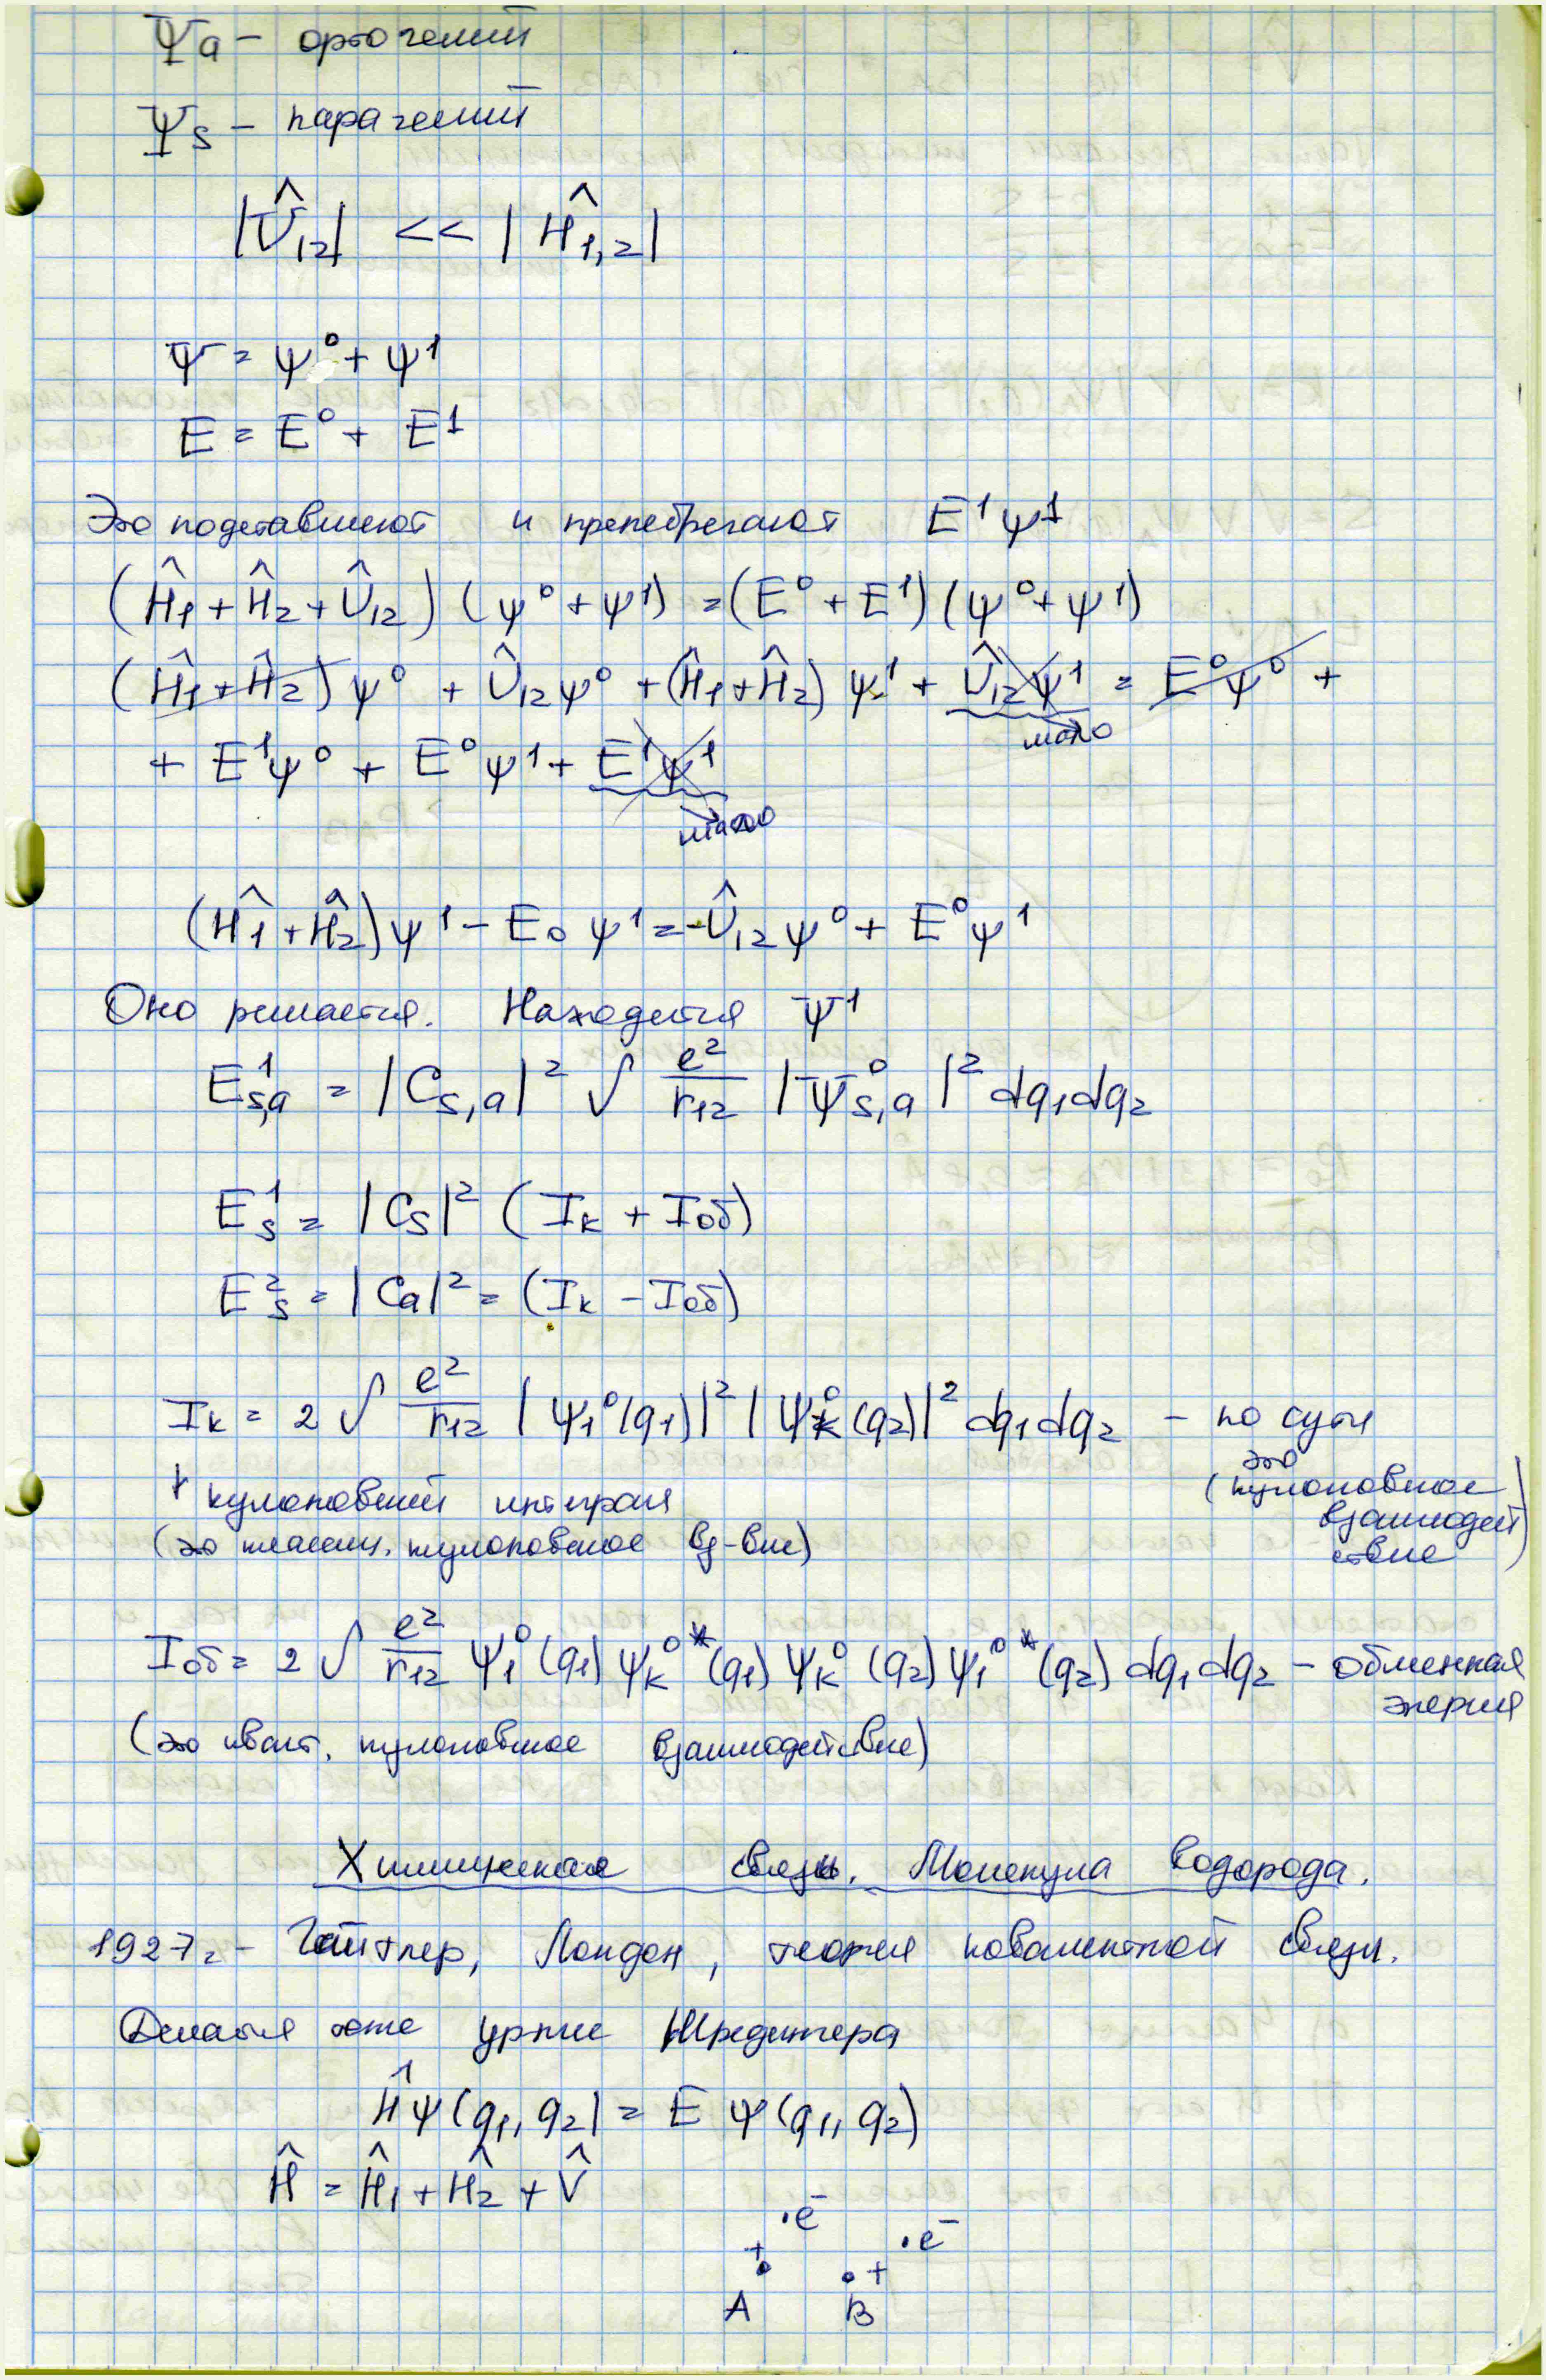
\includegraphics[max size={\textwidth}{0.995\textheight}]{jpg/18.jpg}%
\newpage%
%
%
\phantomsection\addcontentsline{toc}{section}{\textit{Основы физики твердого тела}}%
\phantomsection\addcontentsline{toc}{subsection}{Квантовая статистика}%
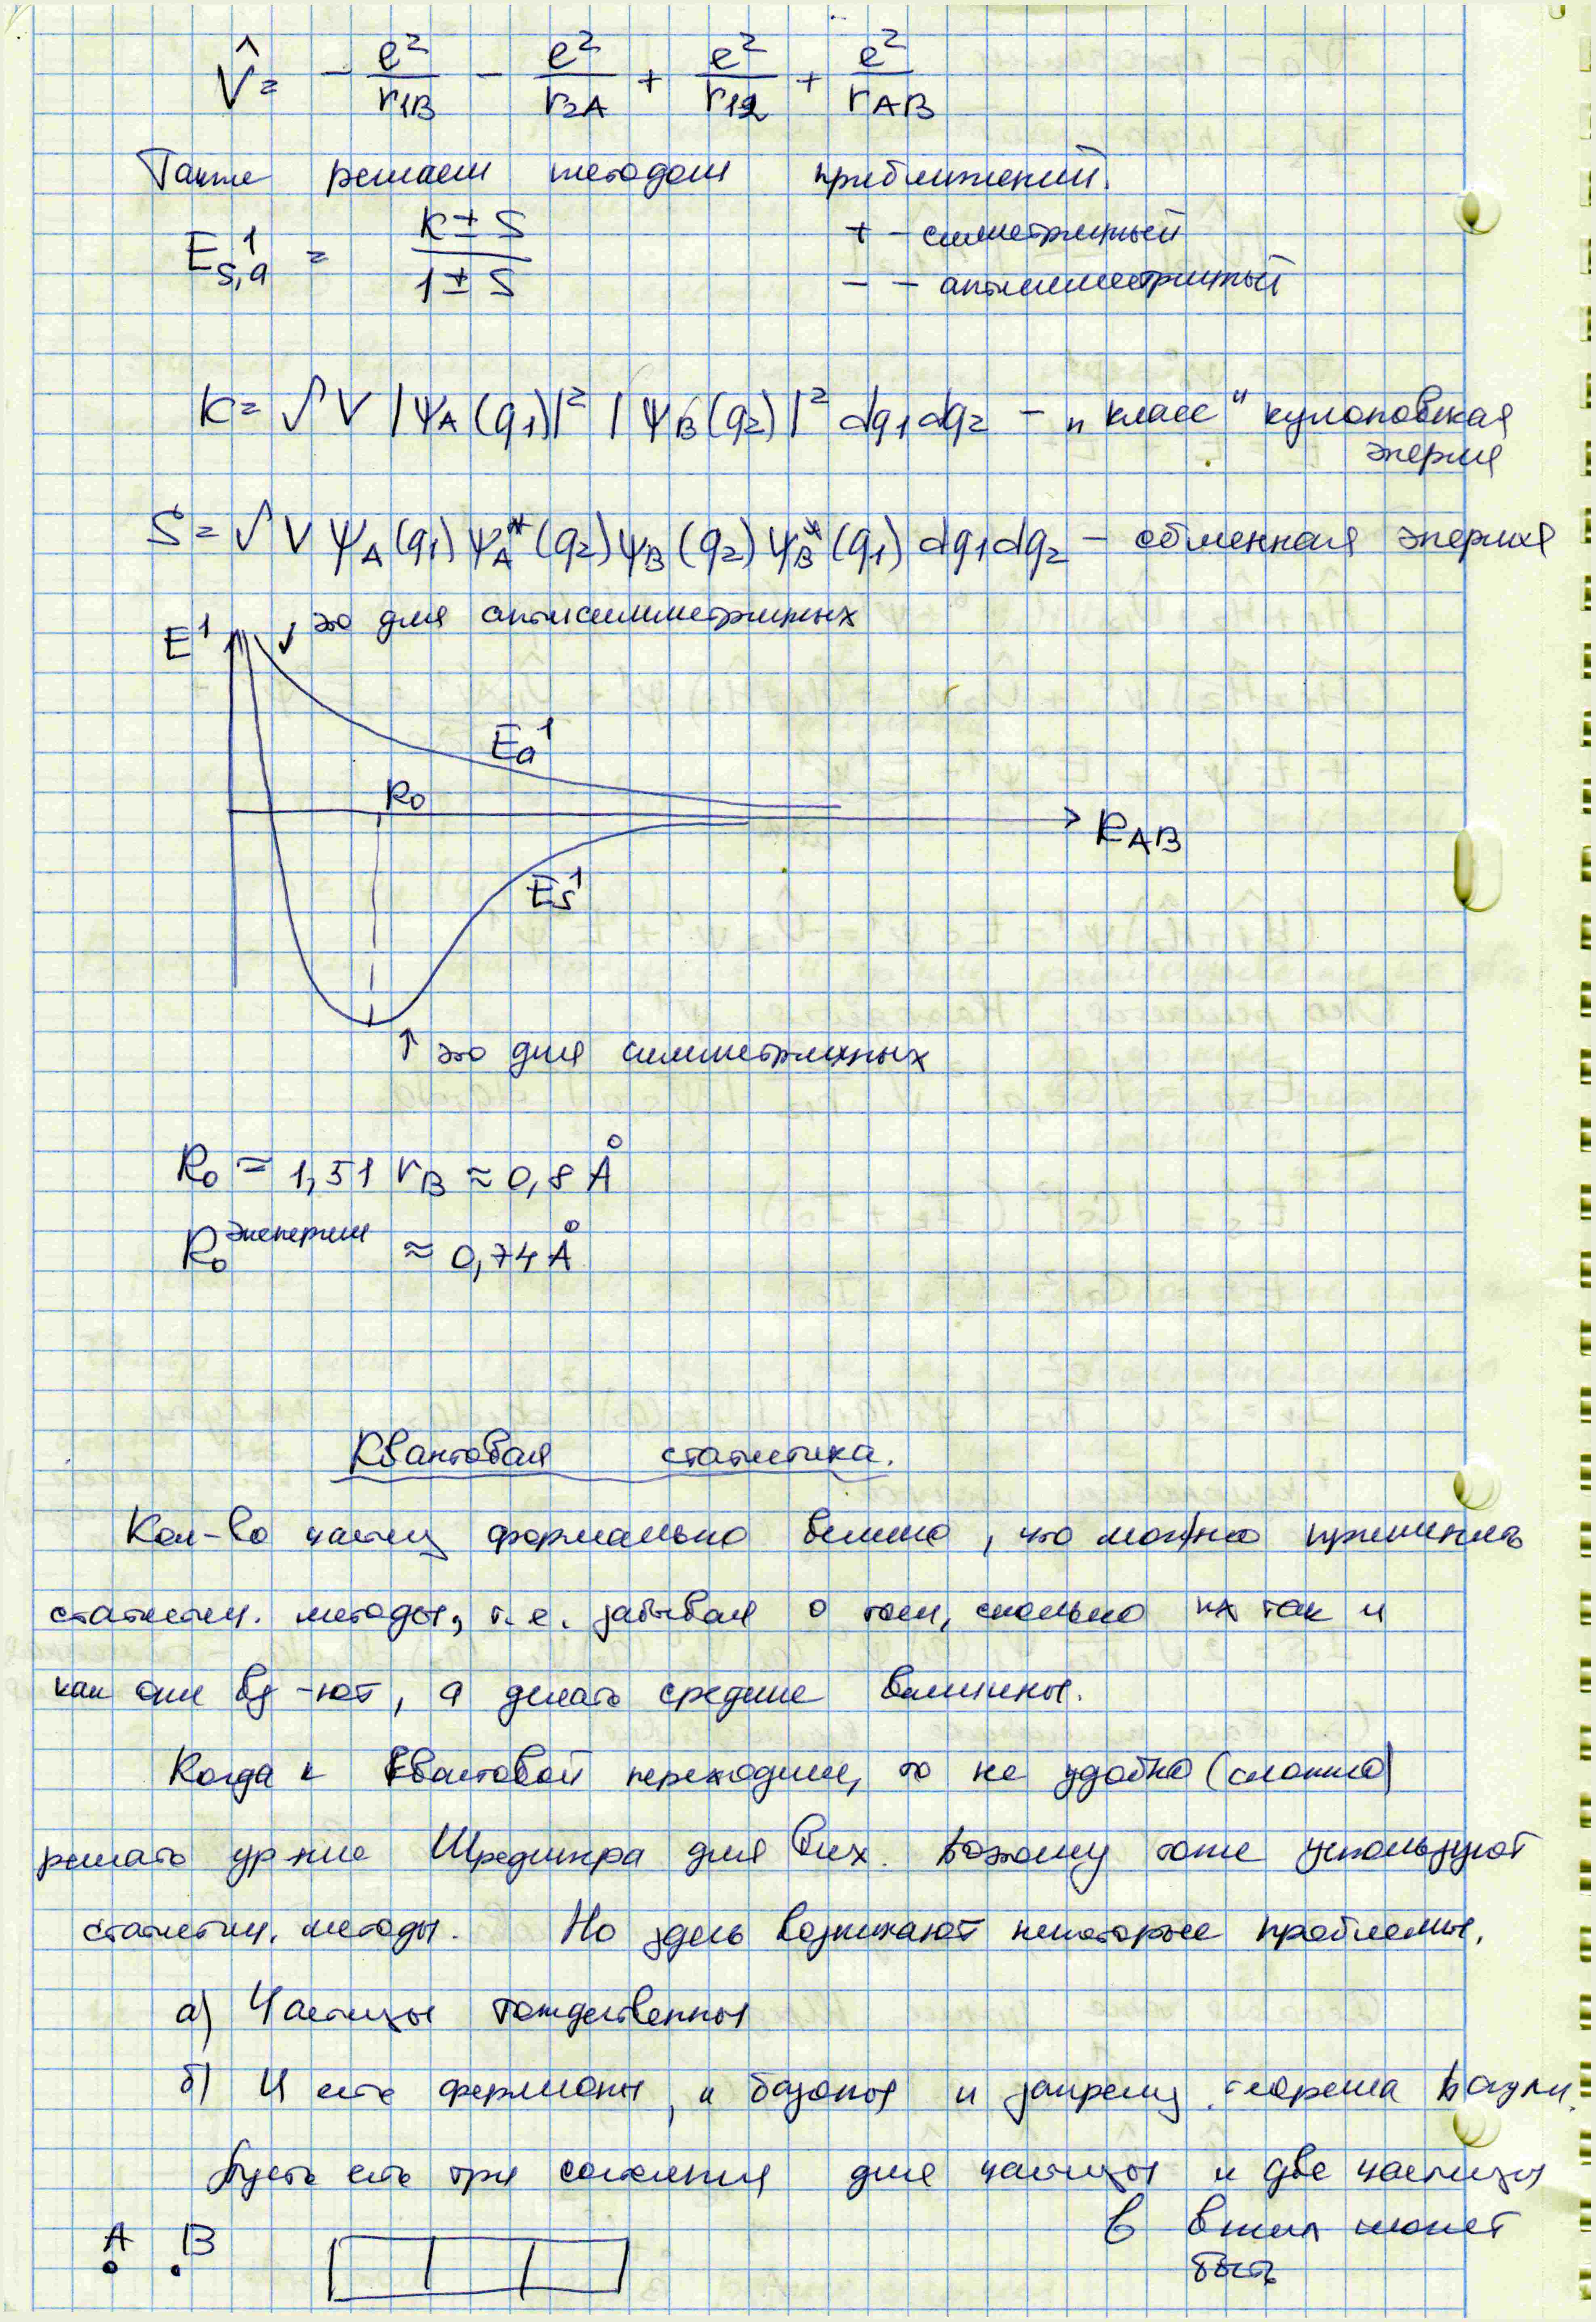
\includegraphics[max size={\textwidth}{0.995\textheight}]{jpg/19.jpg}%
\newpage%
%
%
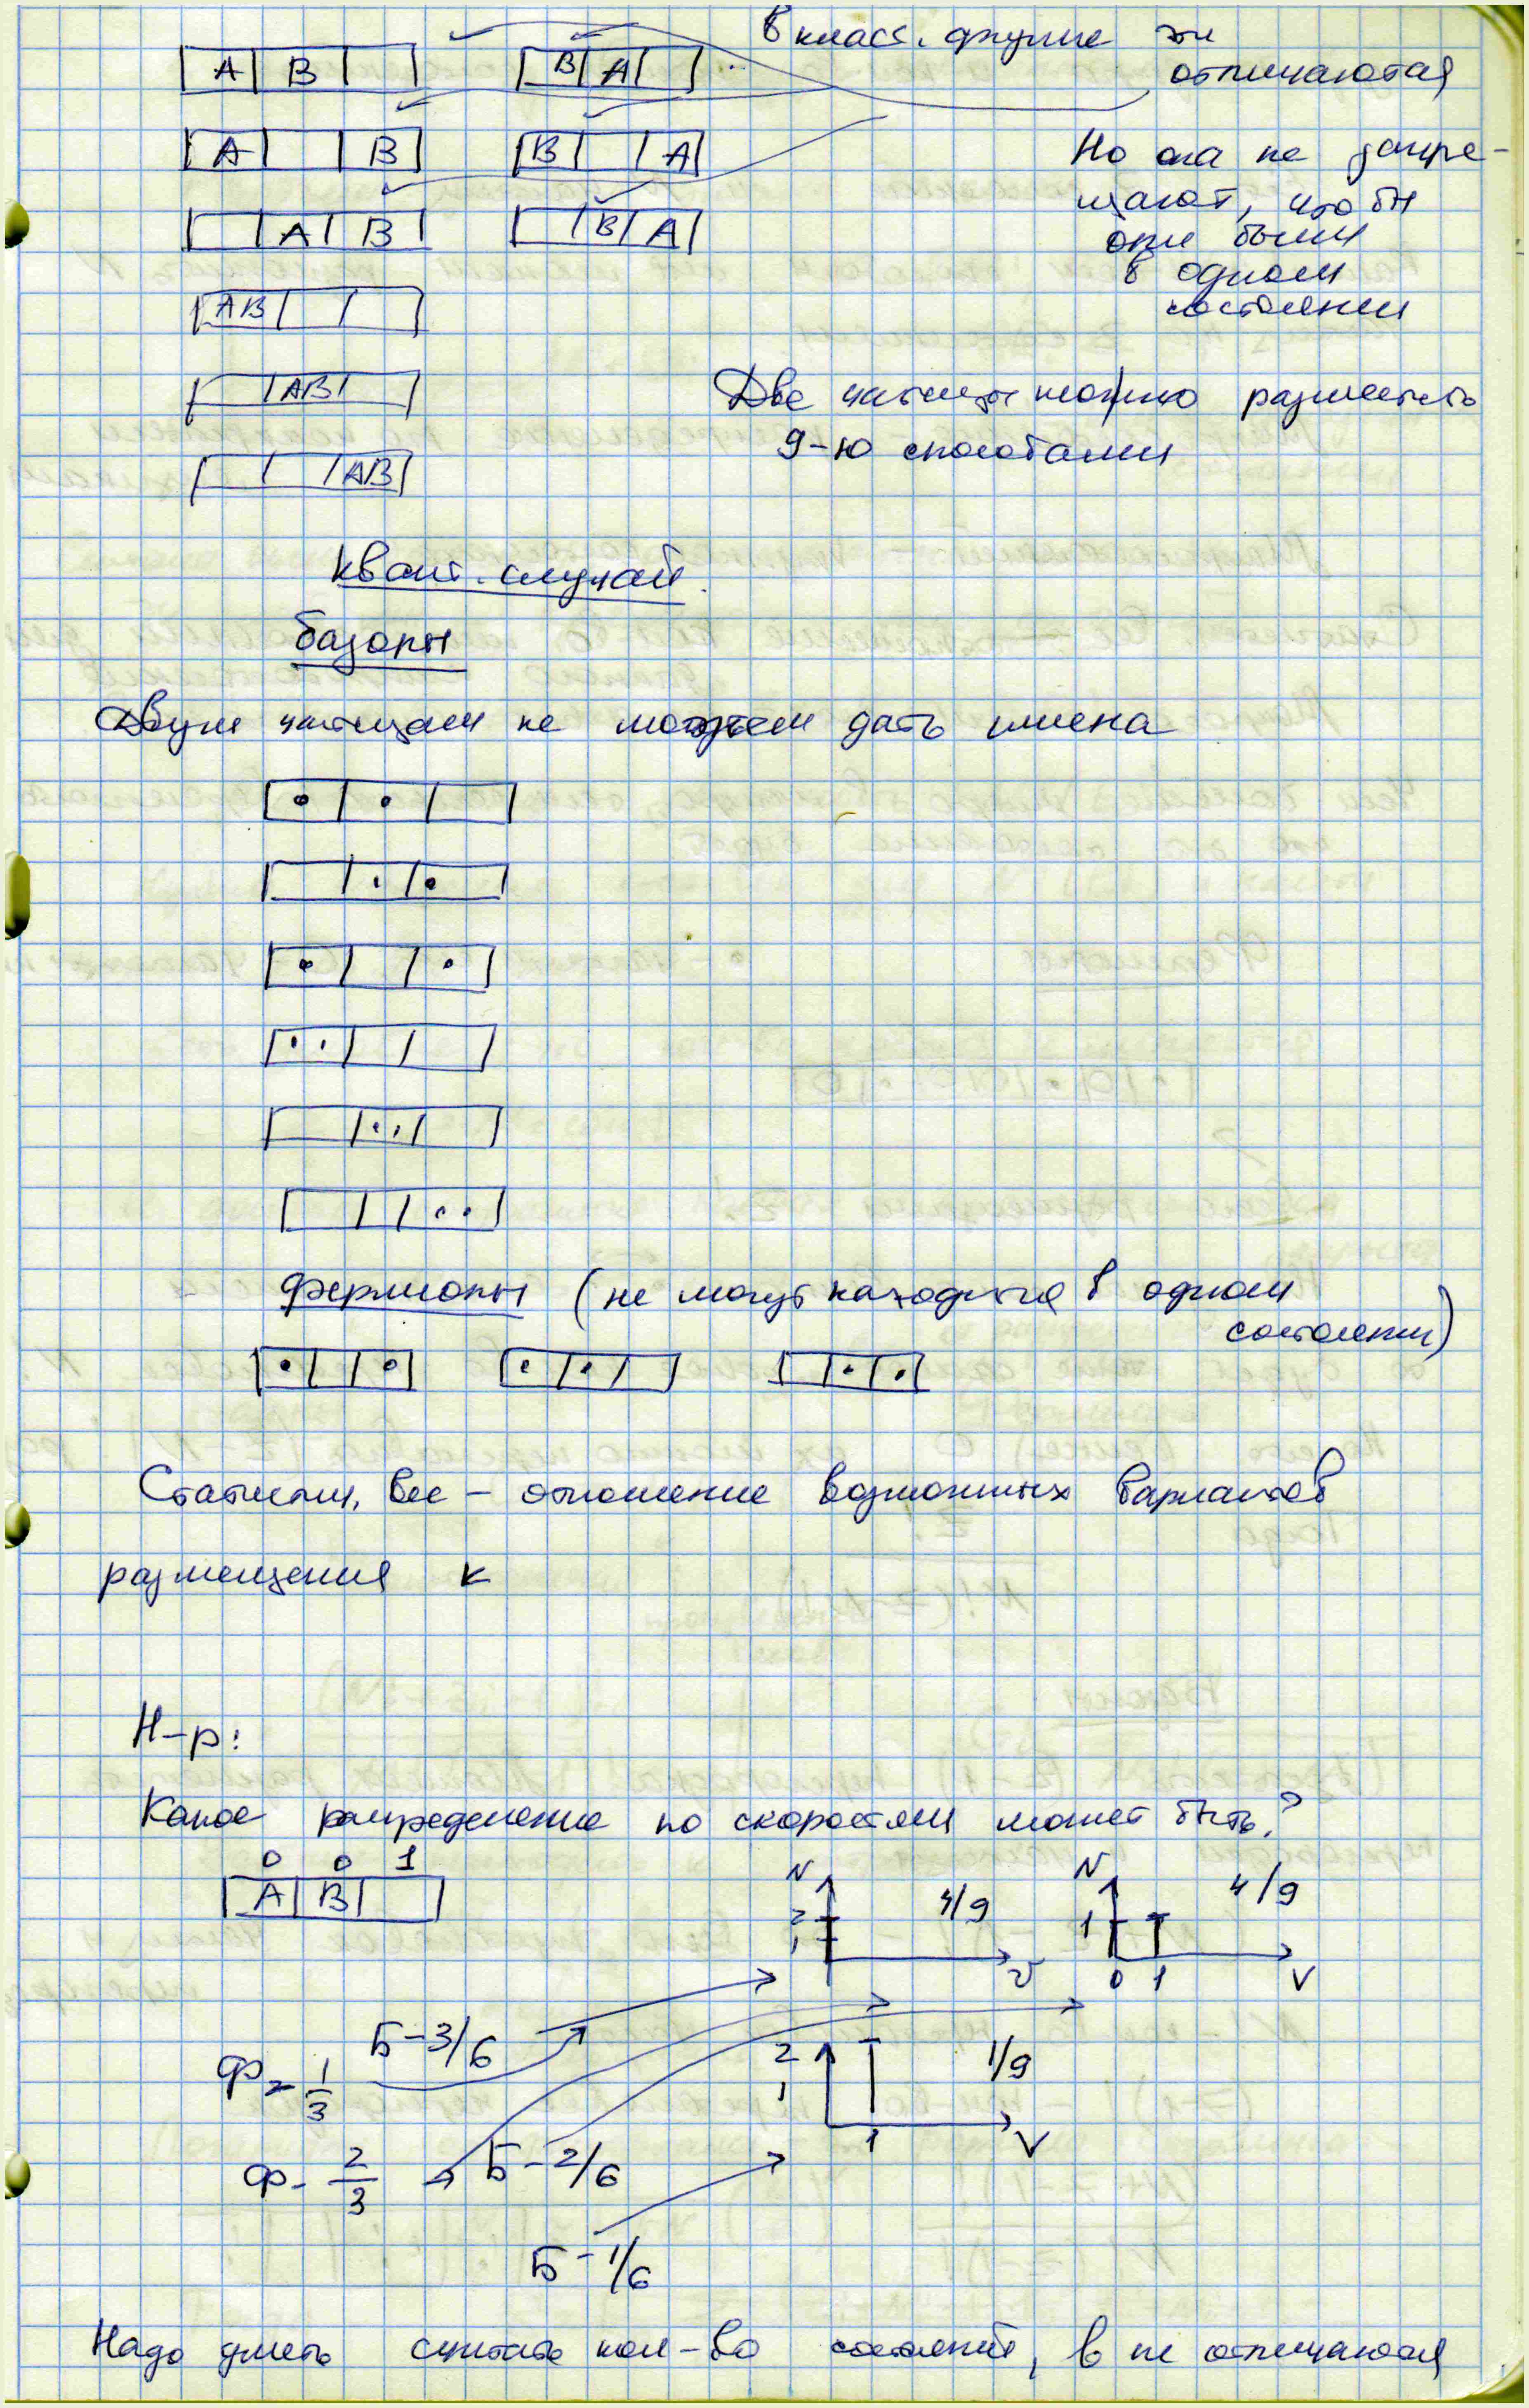
\includegraphics[max size={\textwidth}{0.995\textheight}]{jpg/20.jpg}%
\newpage%
%
%
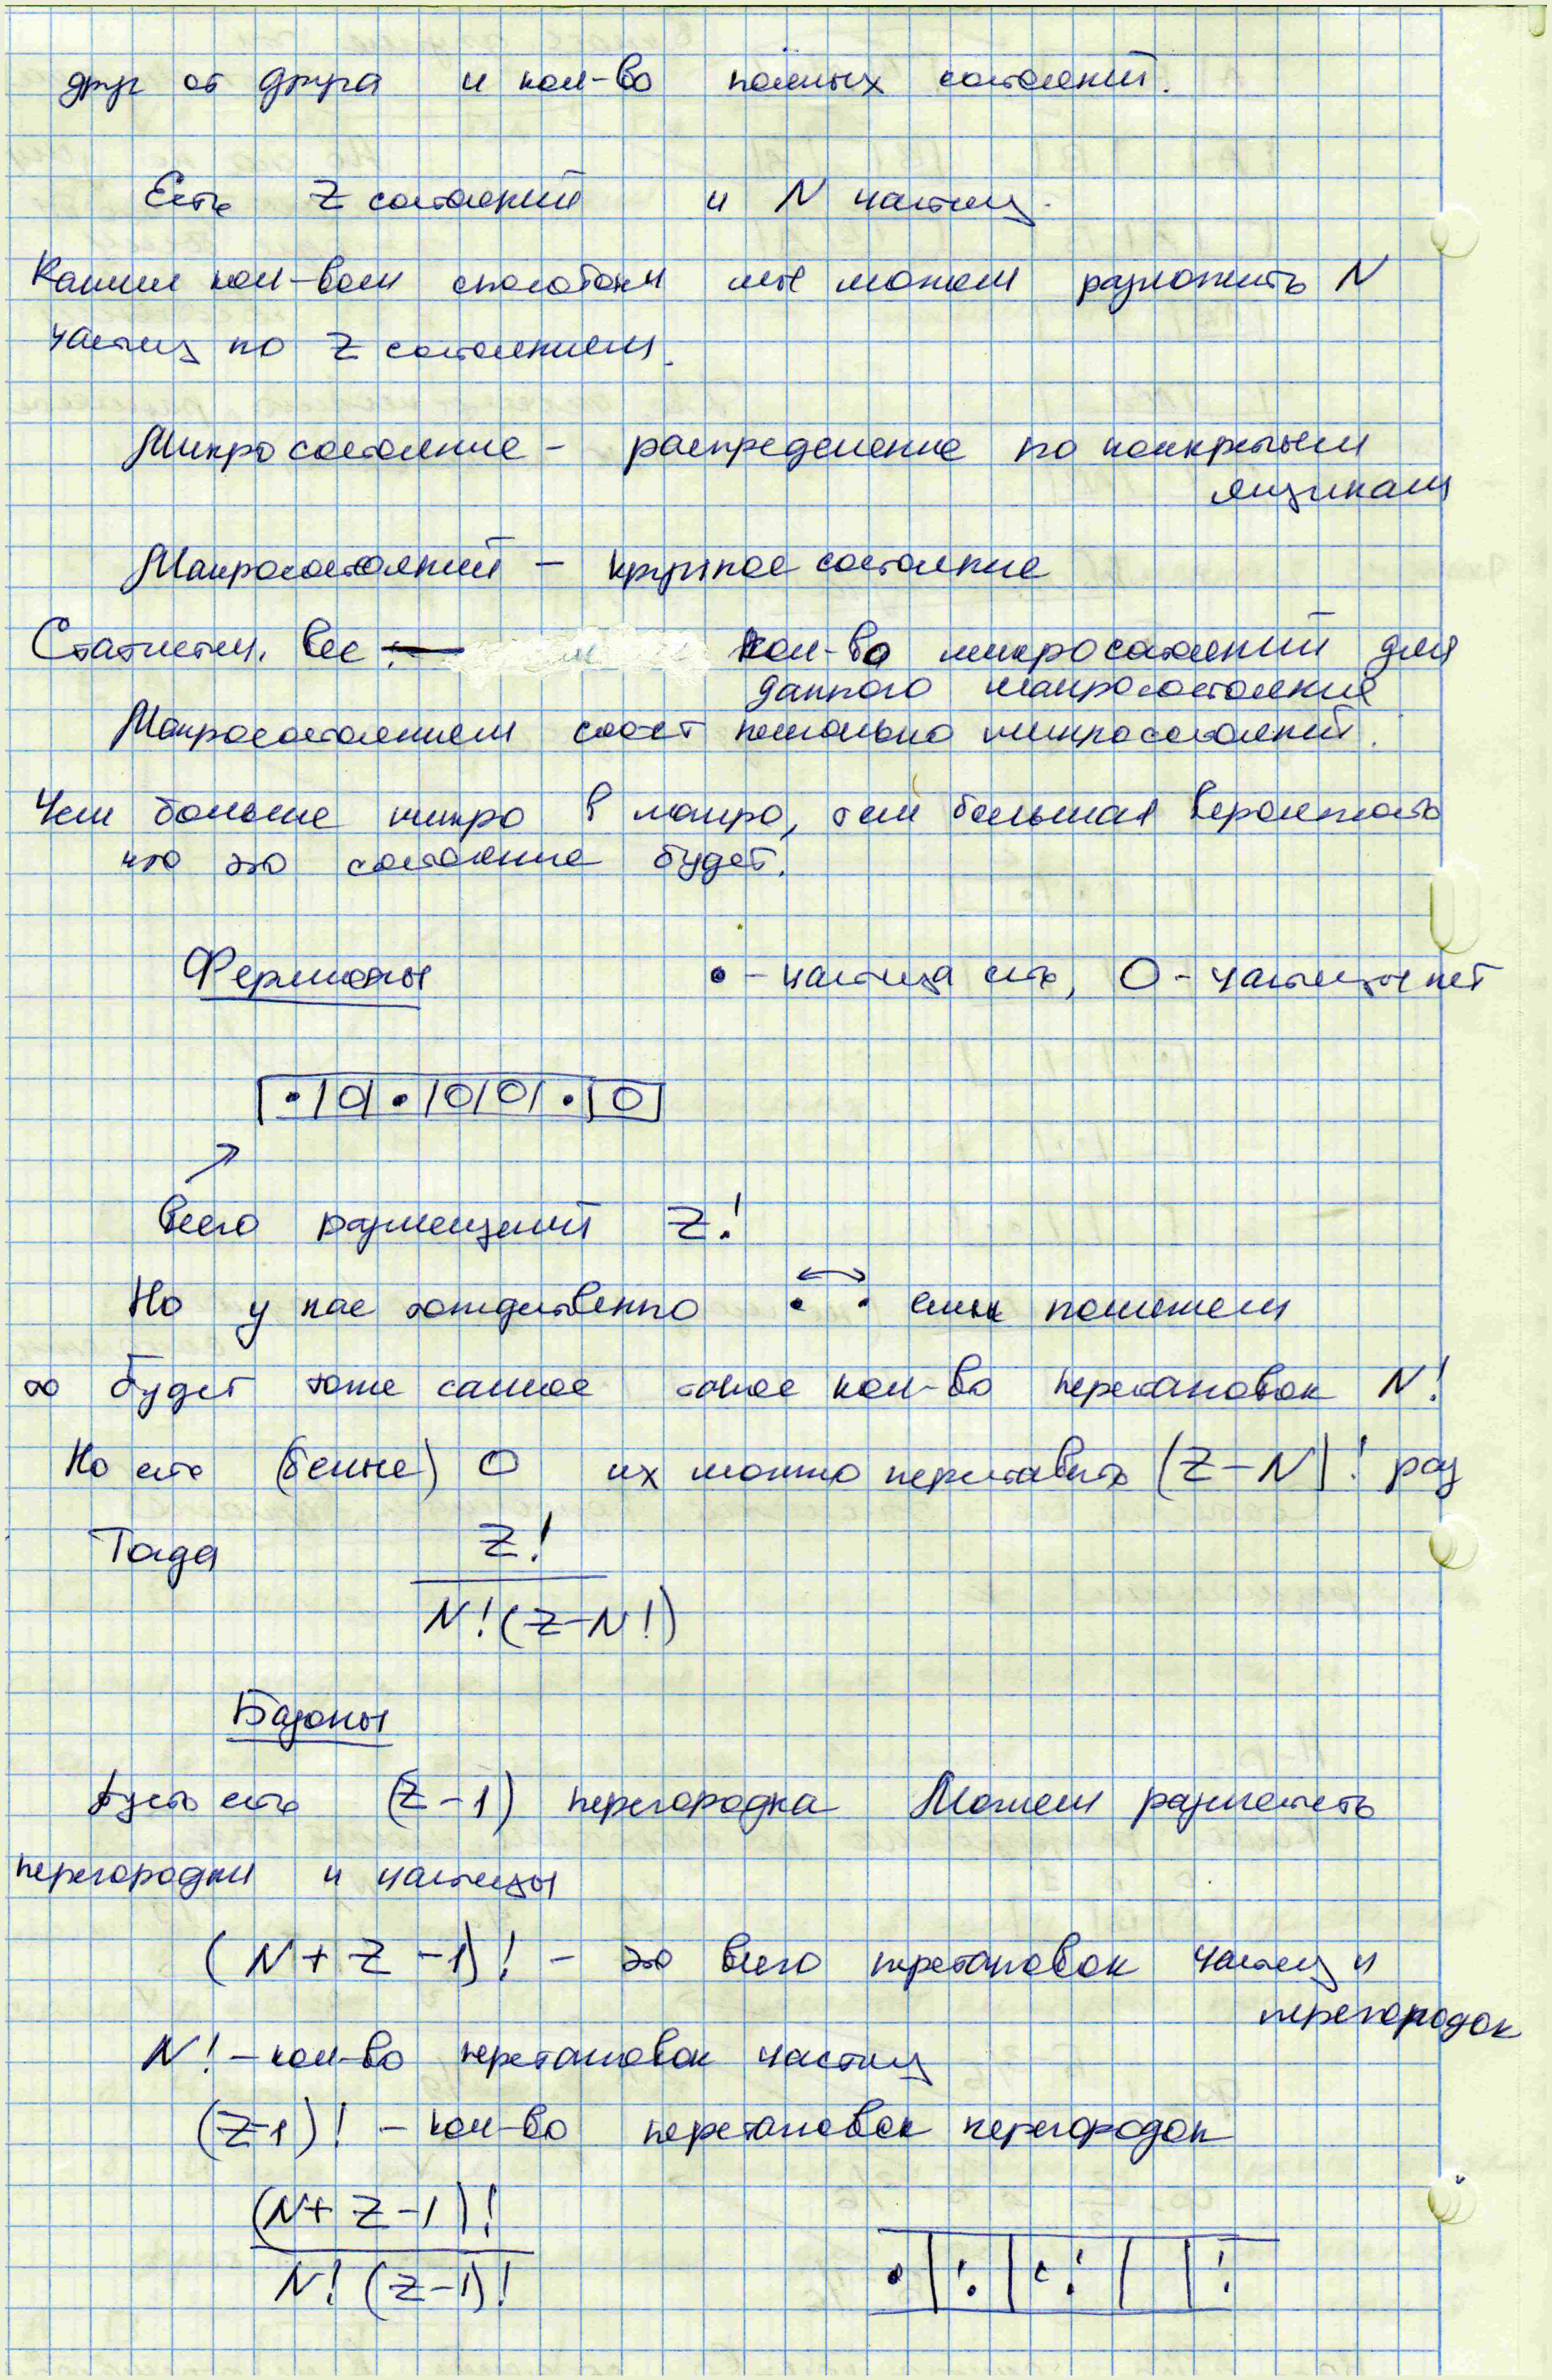
\includegraphics[max size={\textwidth}{0.995\textheight}]{jpg/21.jpg}%
\newpage%
%
%
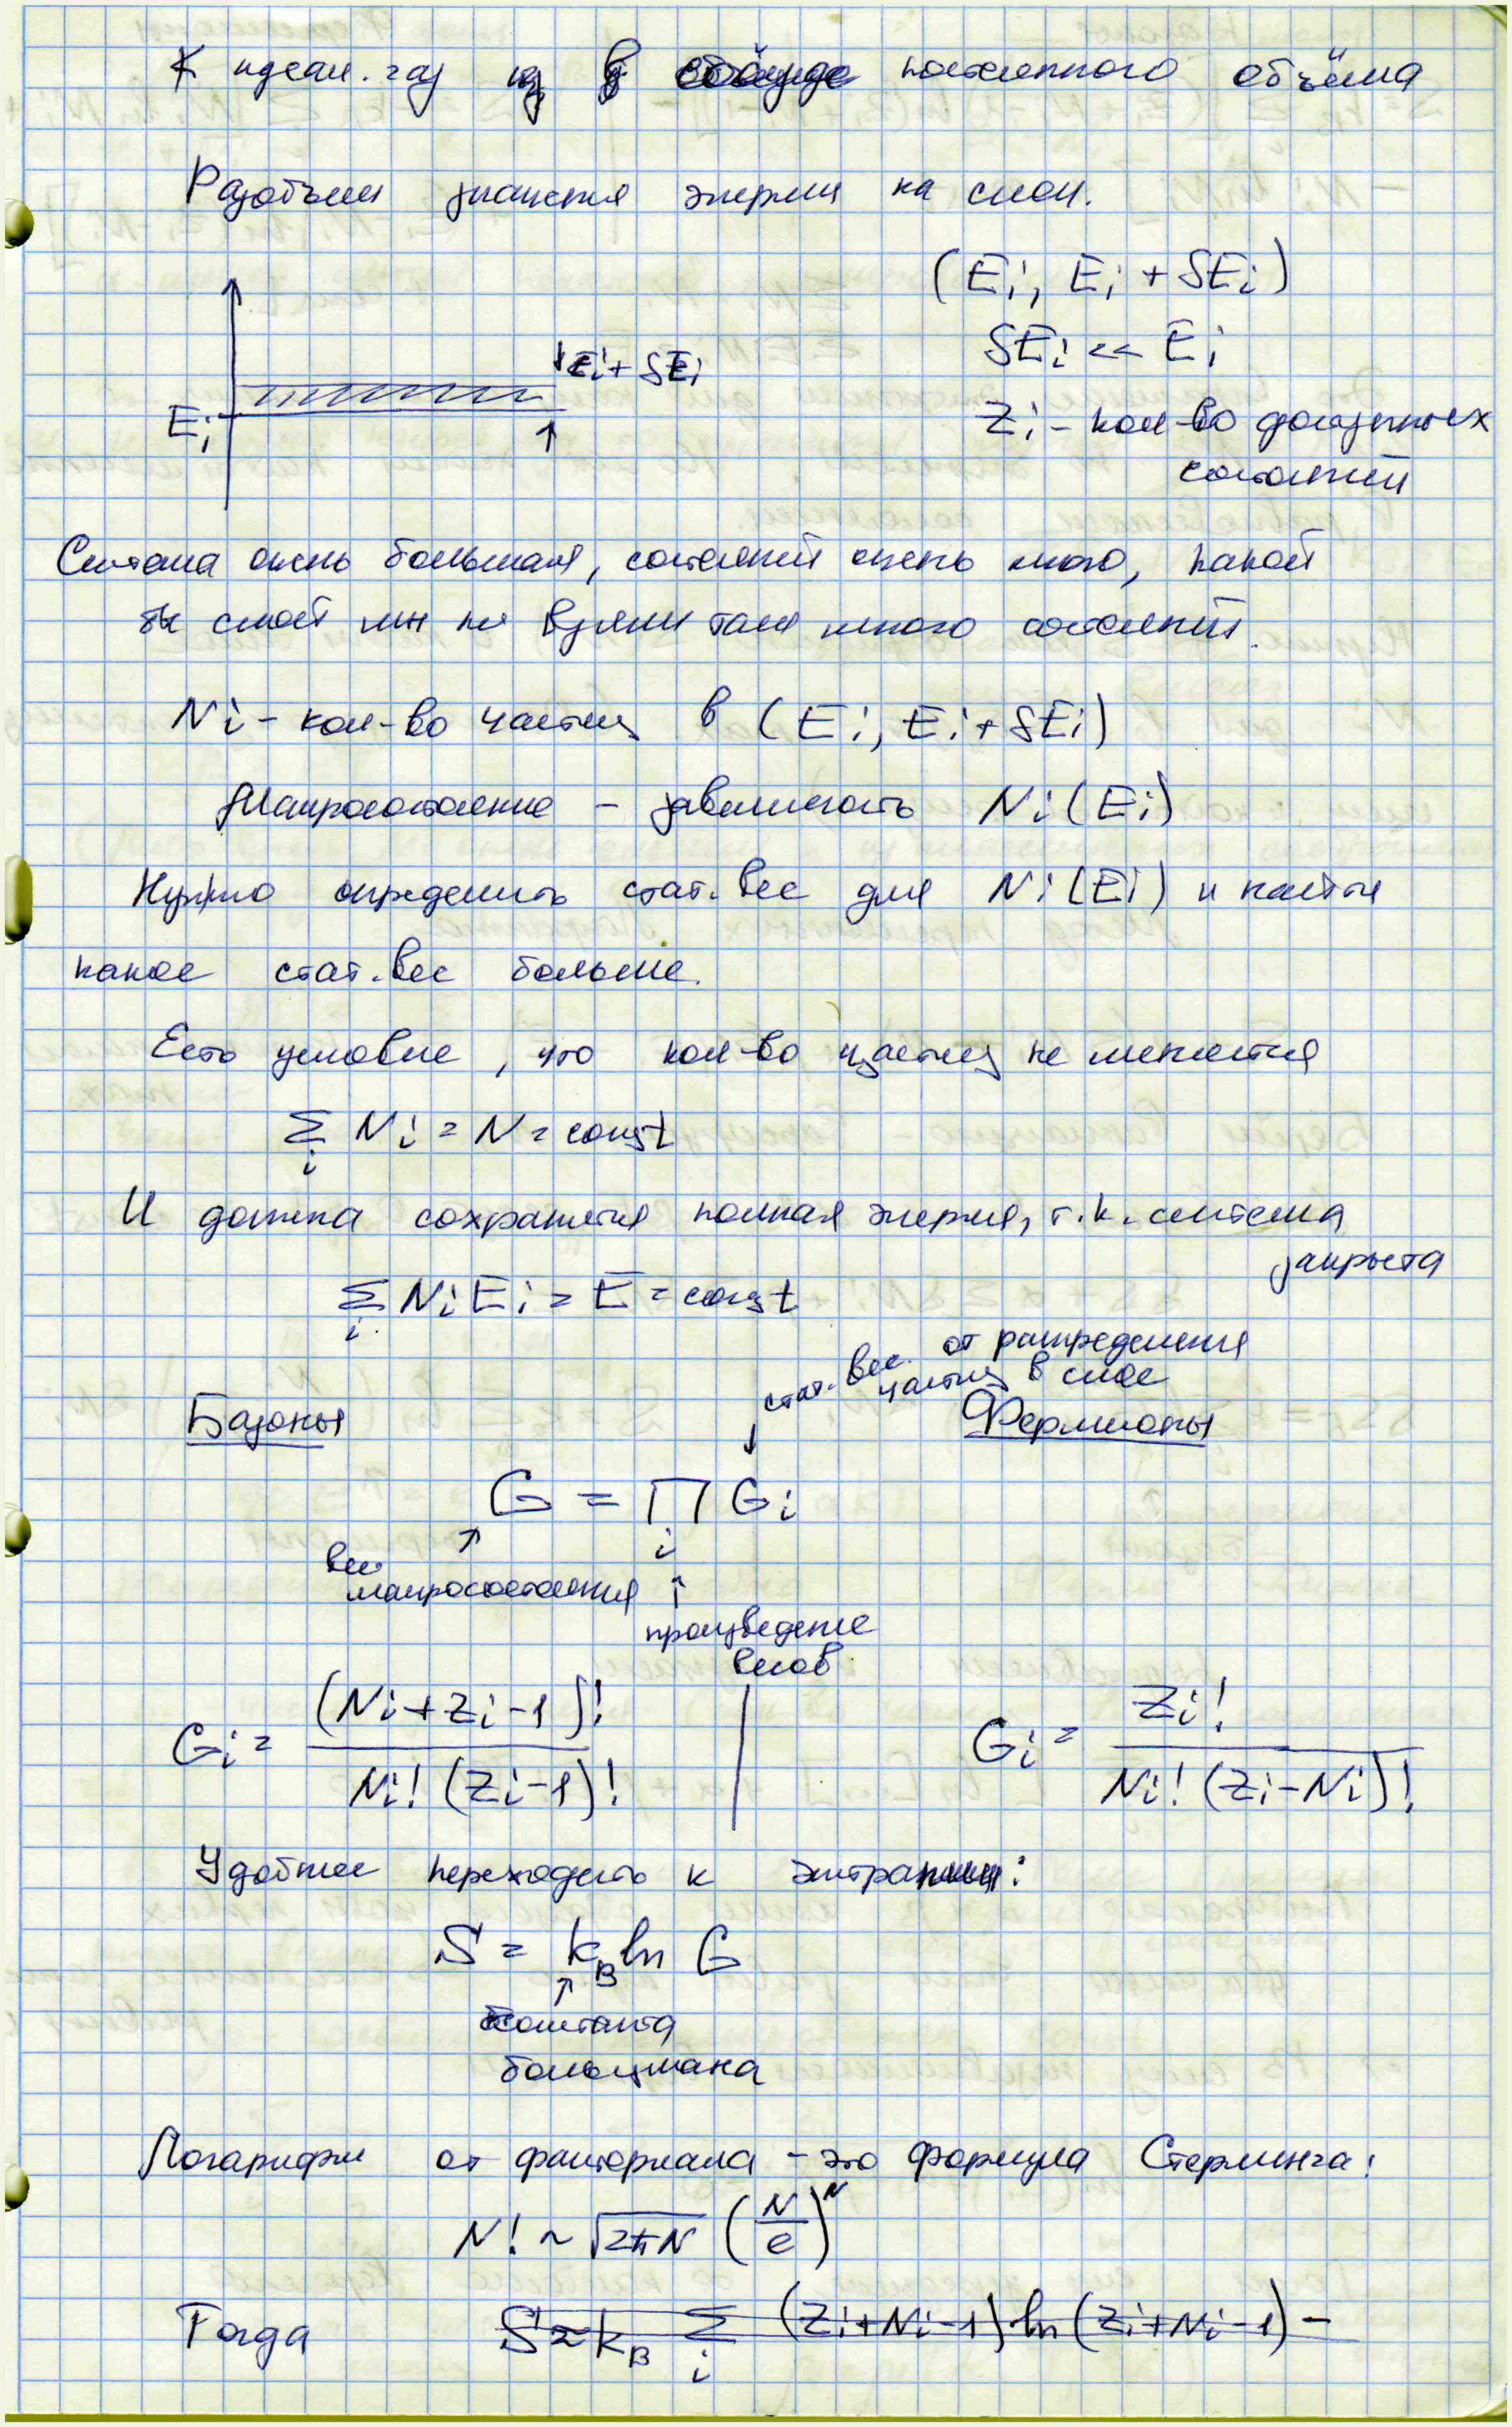
\includegraphics[max size={\textwidth}{0.995\textheight}]{jpg/22.jpg}%
\newpage%
%
%
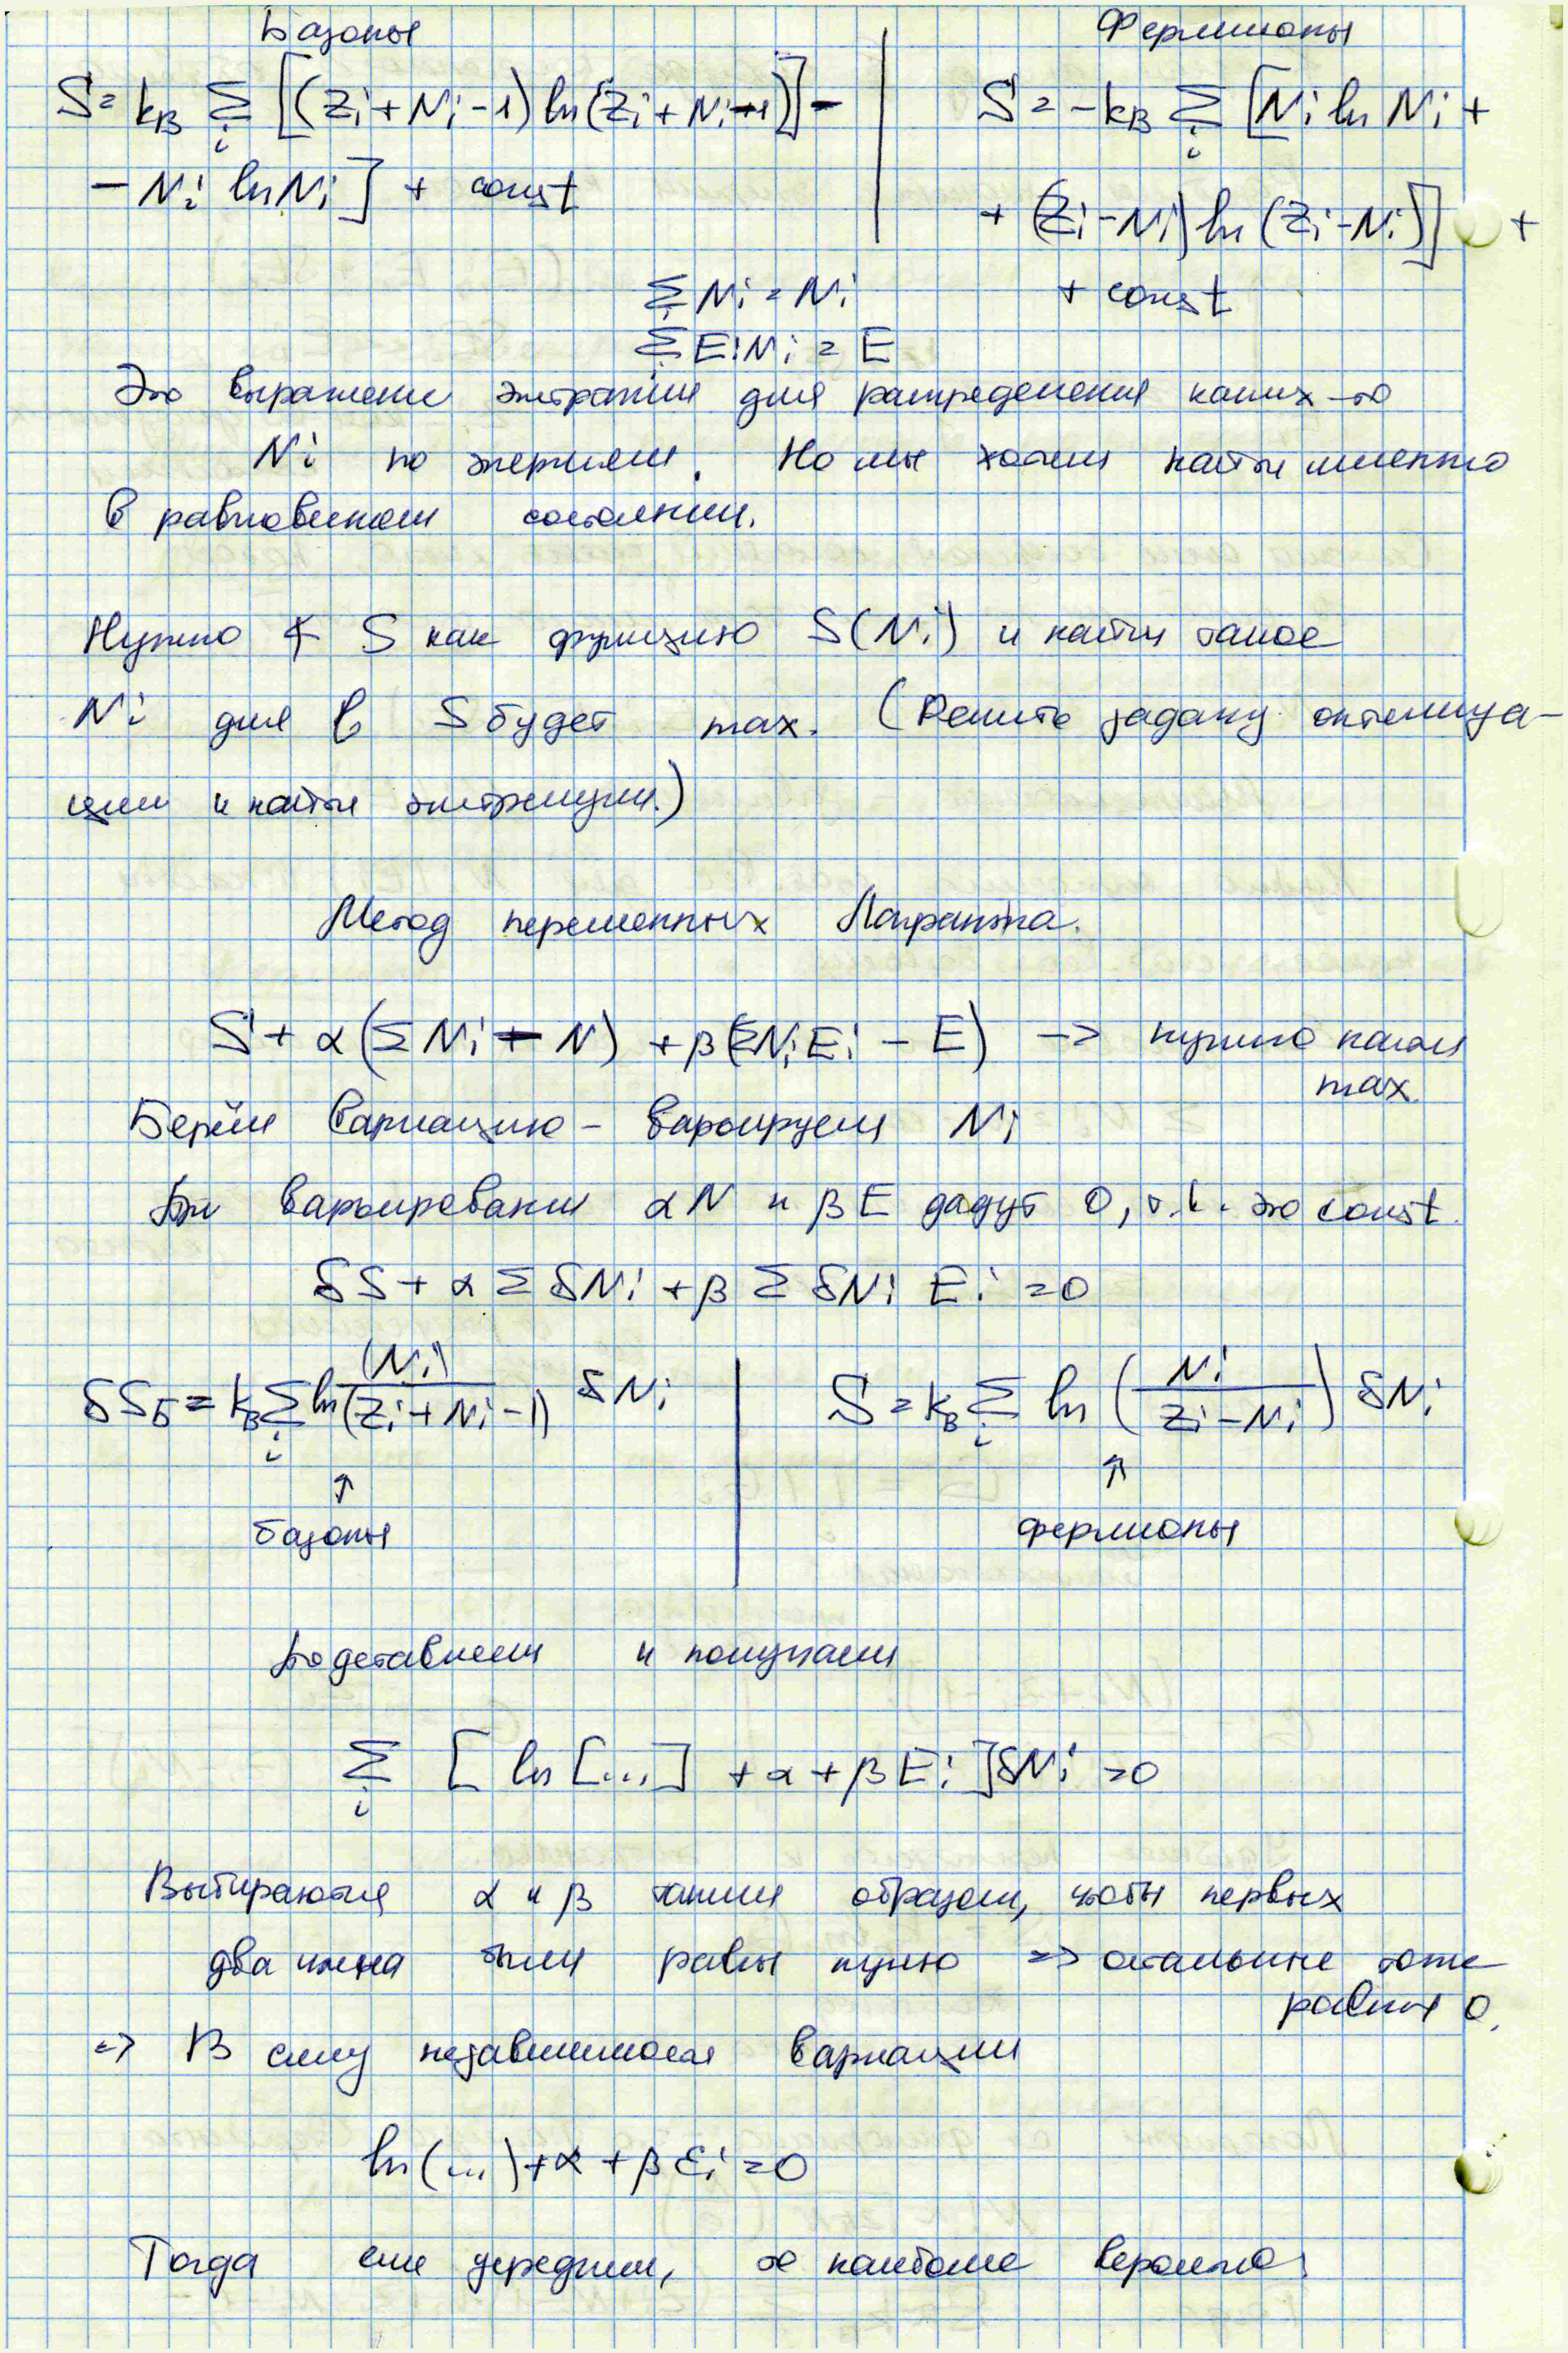
\includegraphics[max size={\textwidth}{0.995\textheight}]{jpg/23.jpg}%
\newpage%
%
%
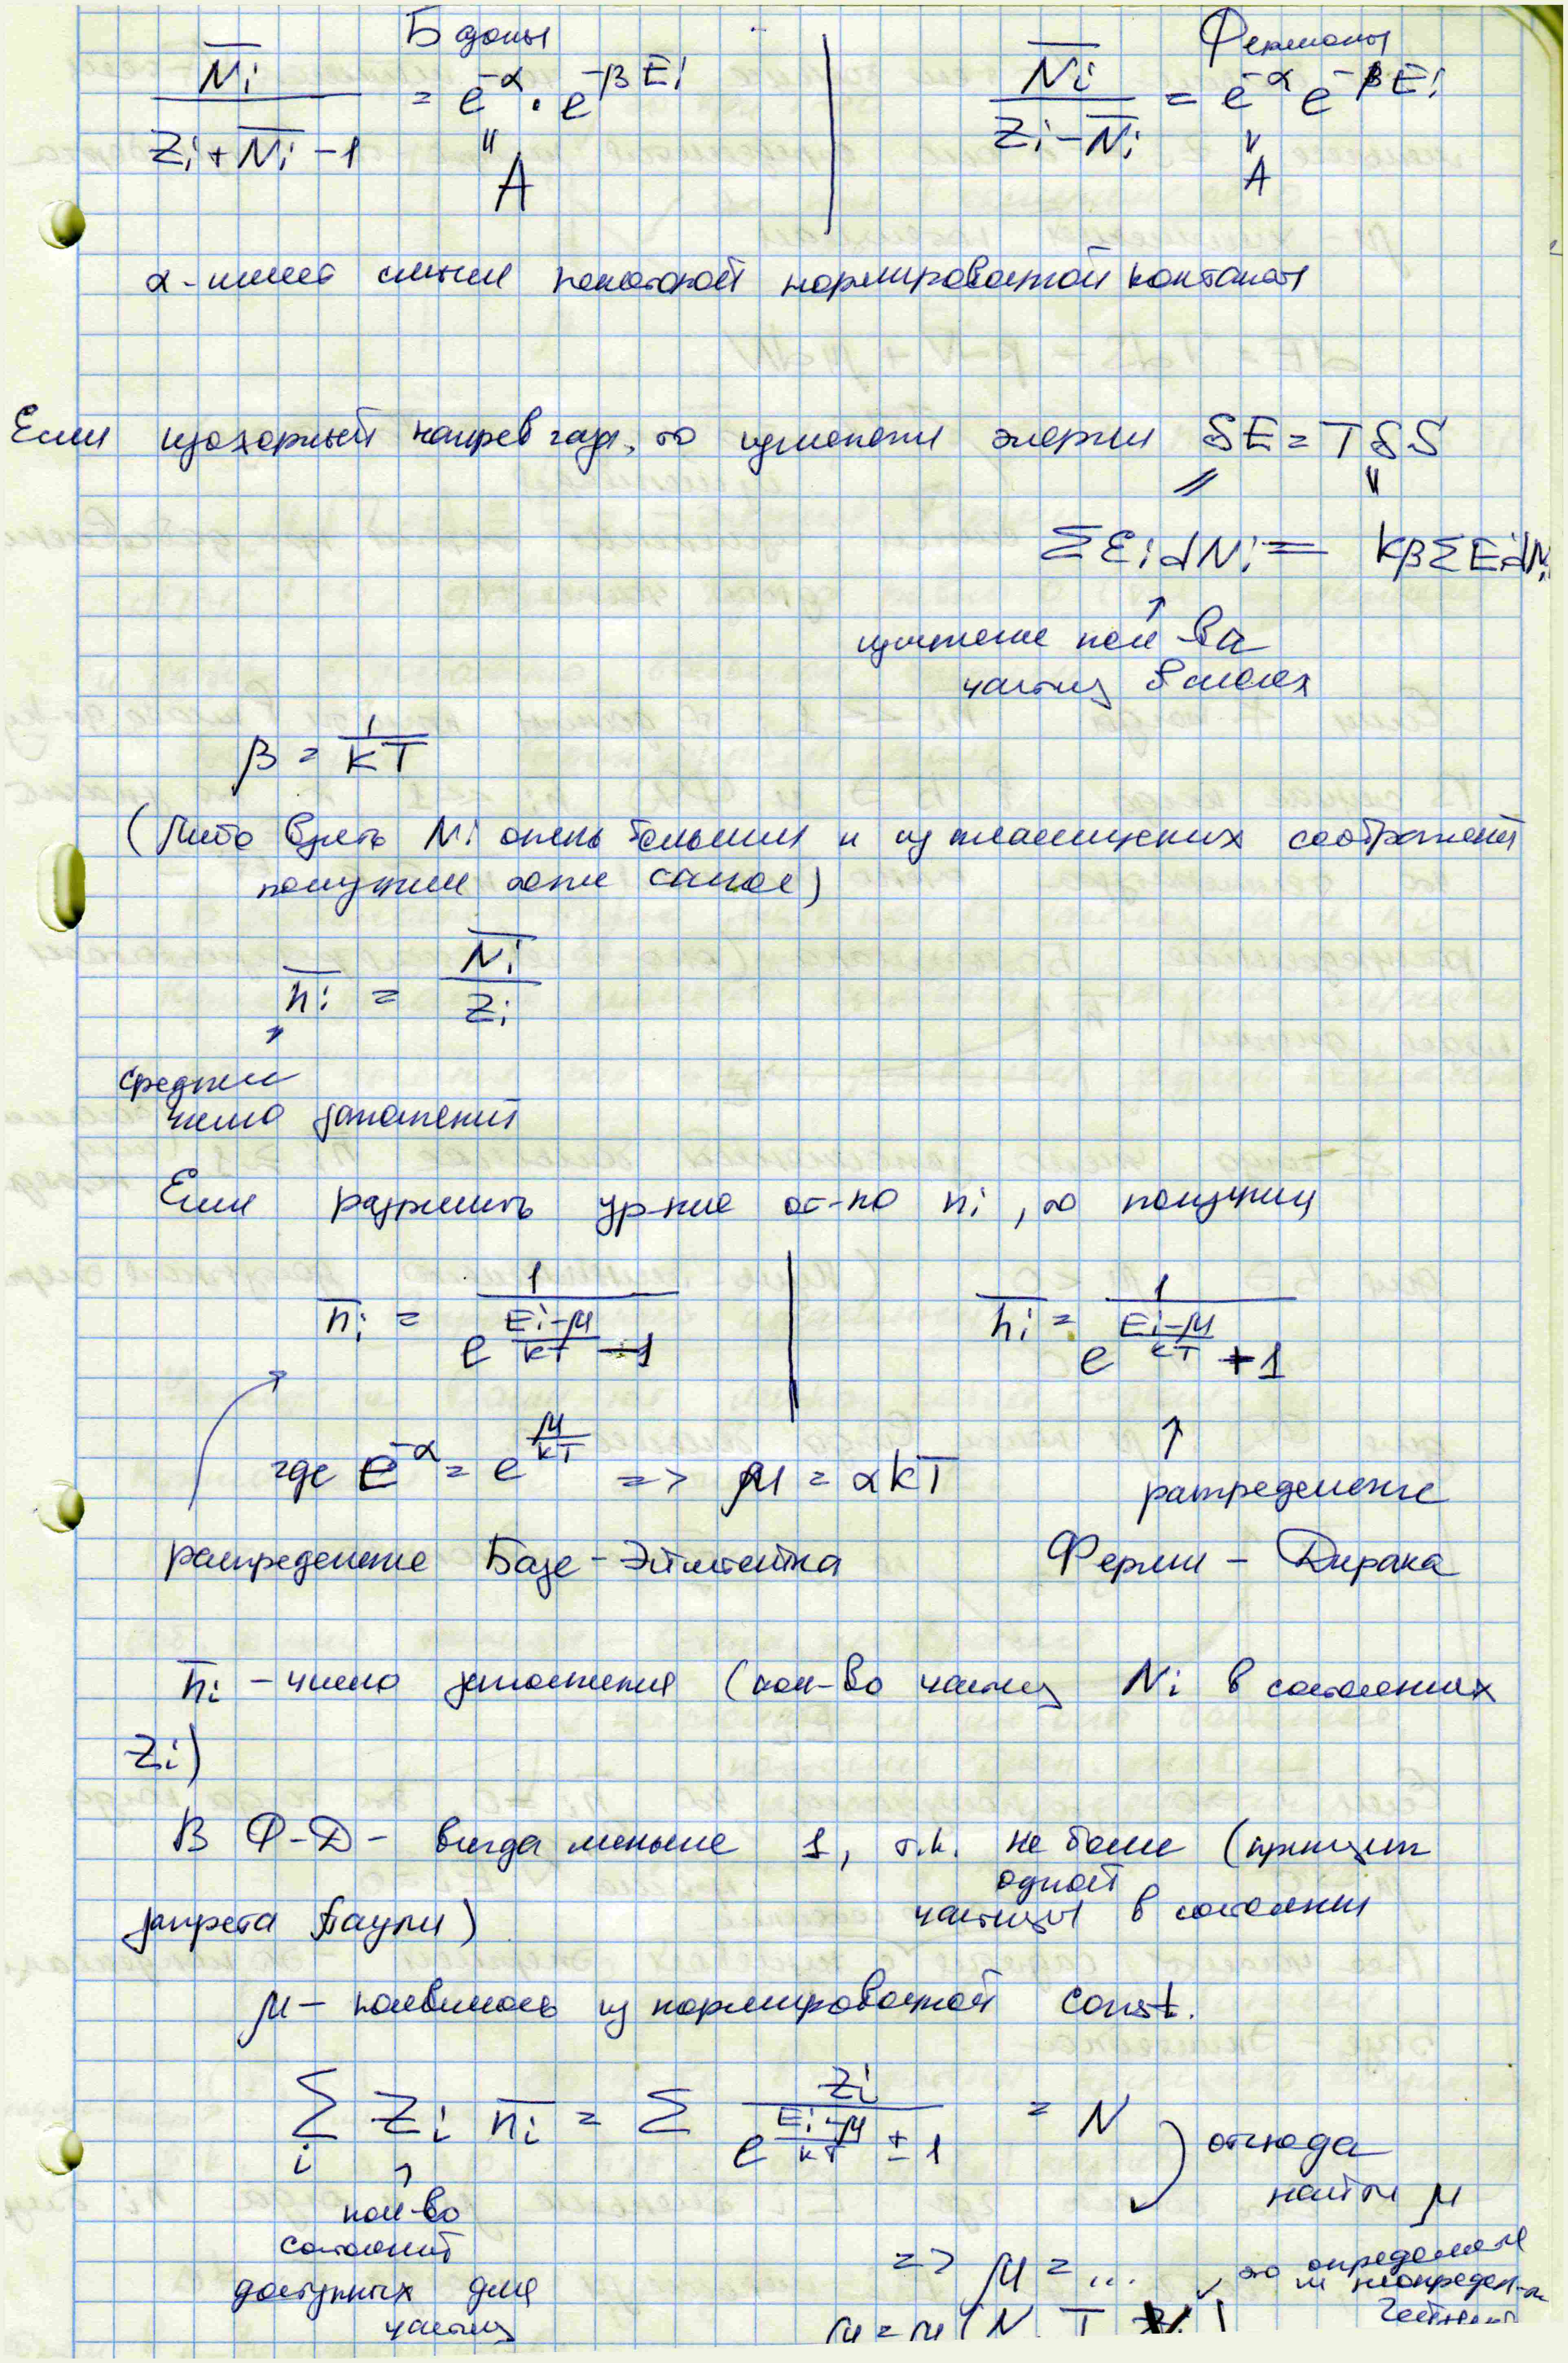
\includegraphics[max size={\textwidth}{0.995\textheight}]{jpg/24.jpg}%
\newpage%
%
%
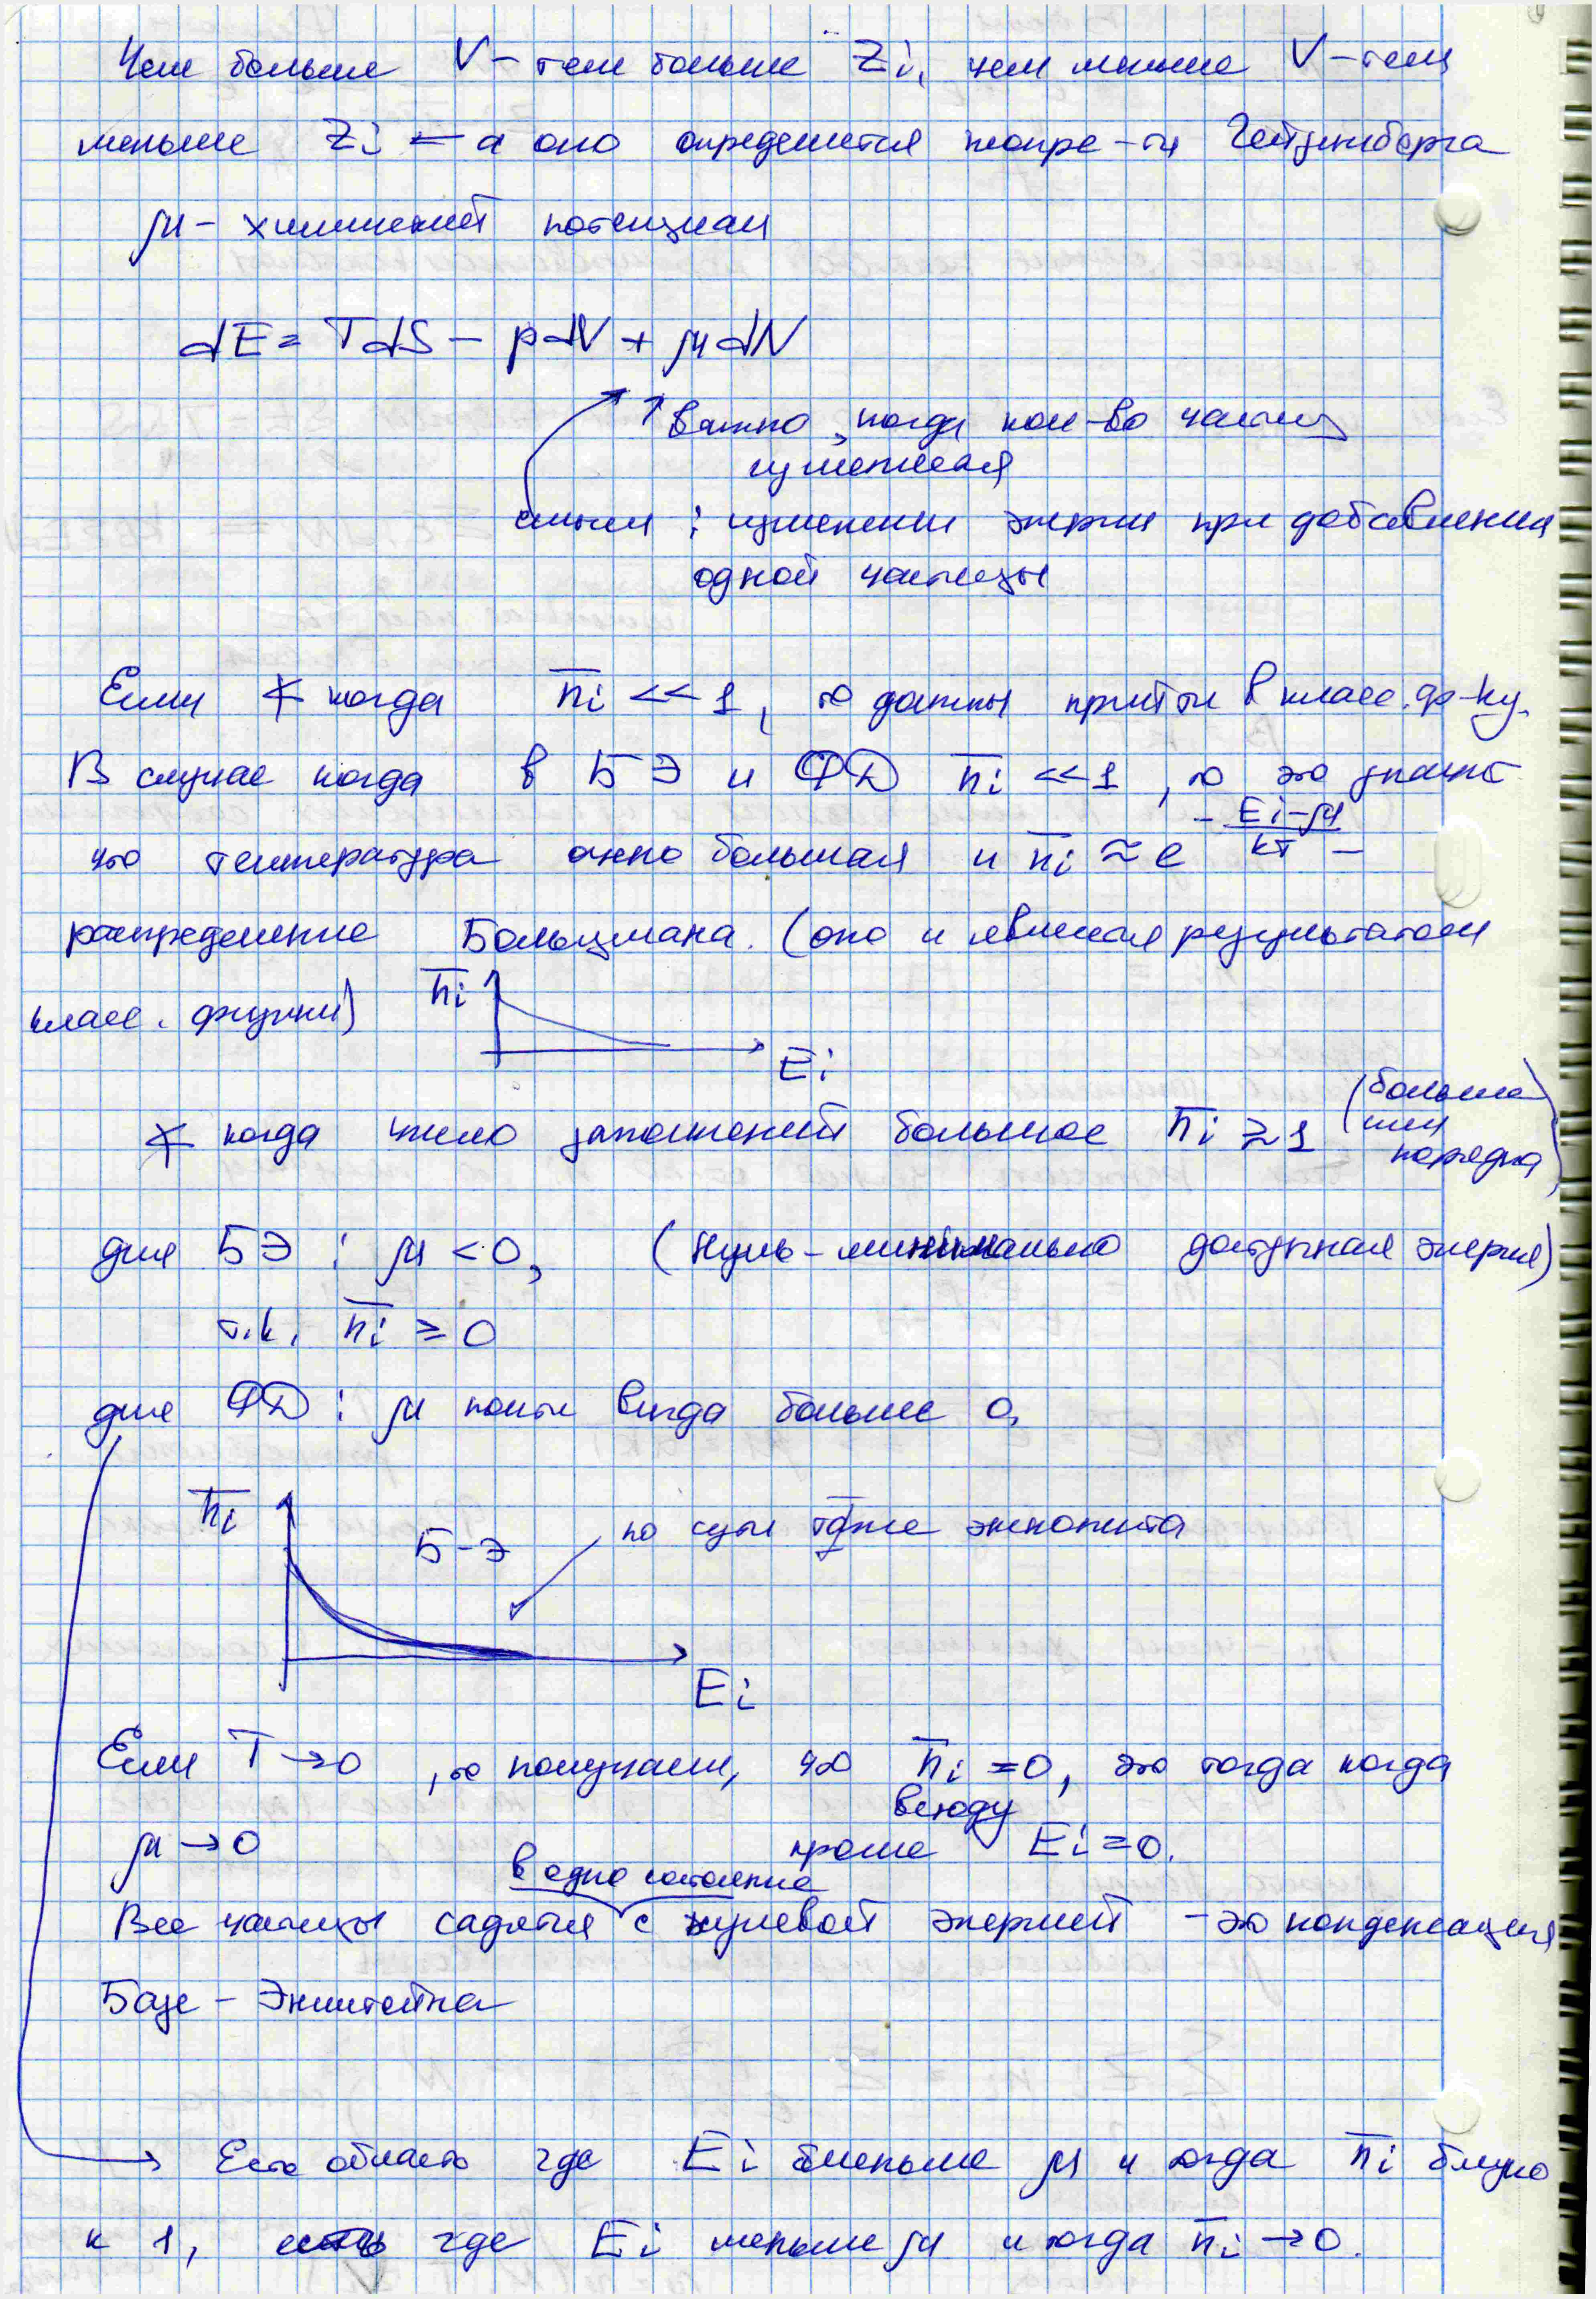
\includegraphics[max size={\textwidth}{0.995\textheight}]{jpg/25.jpg}%
\newpage%
%
%
\phantomsection\addcontentsline{toc}{subsection}{Вырожденный идеальный газ}%
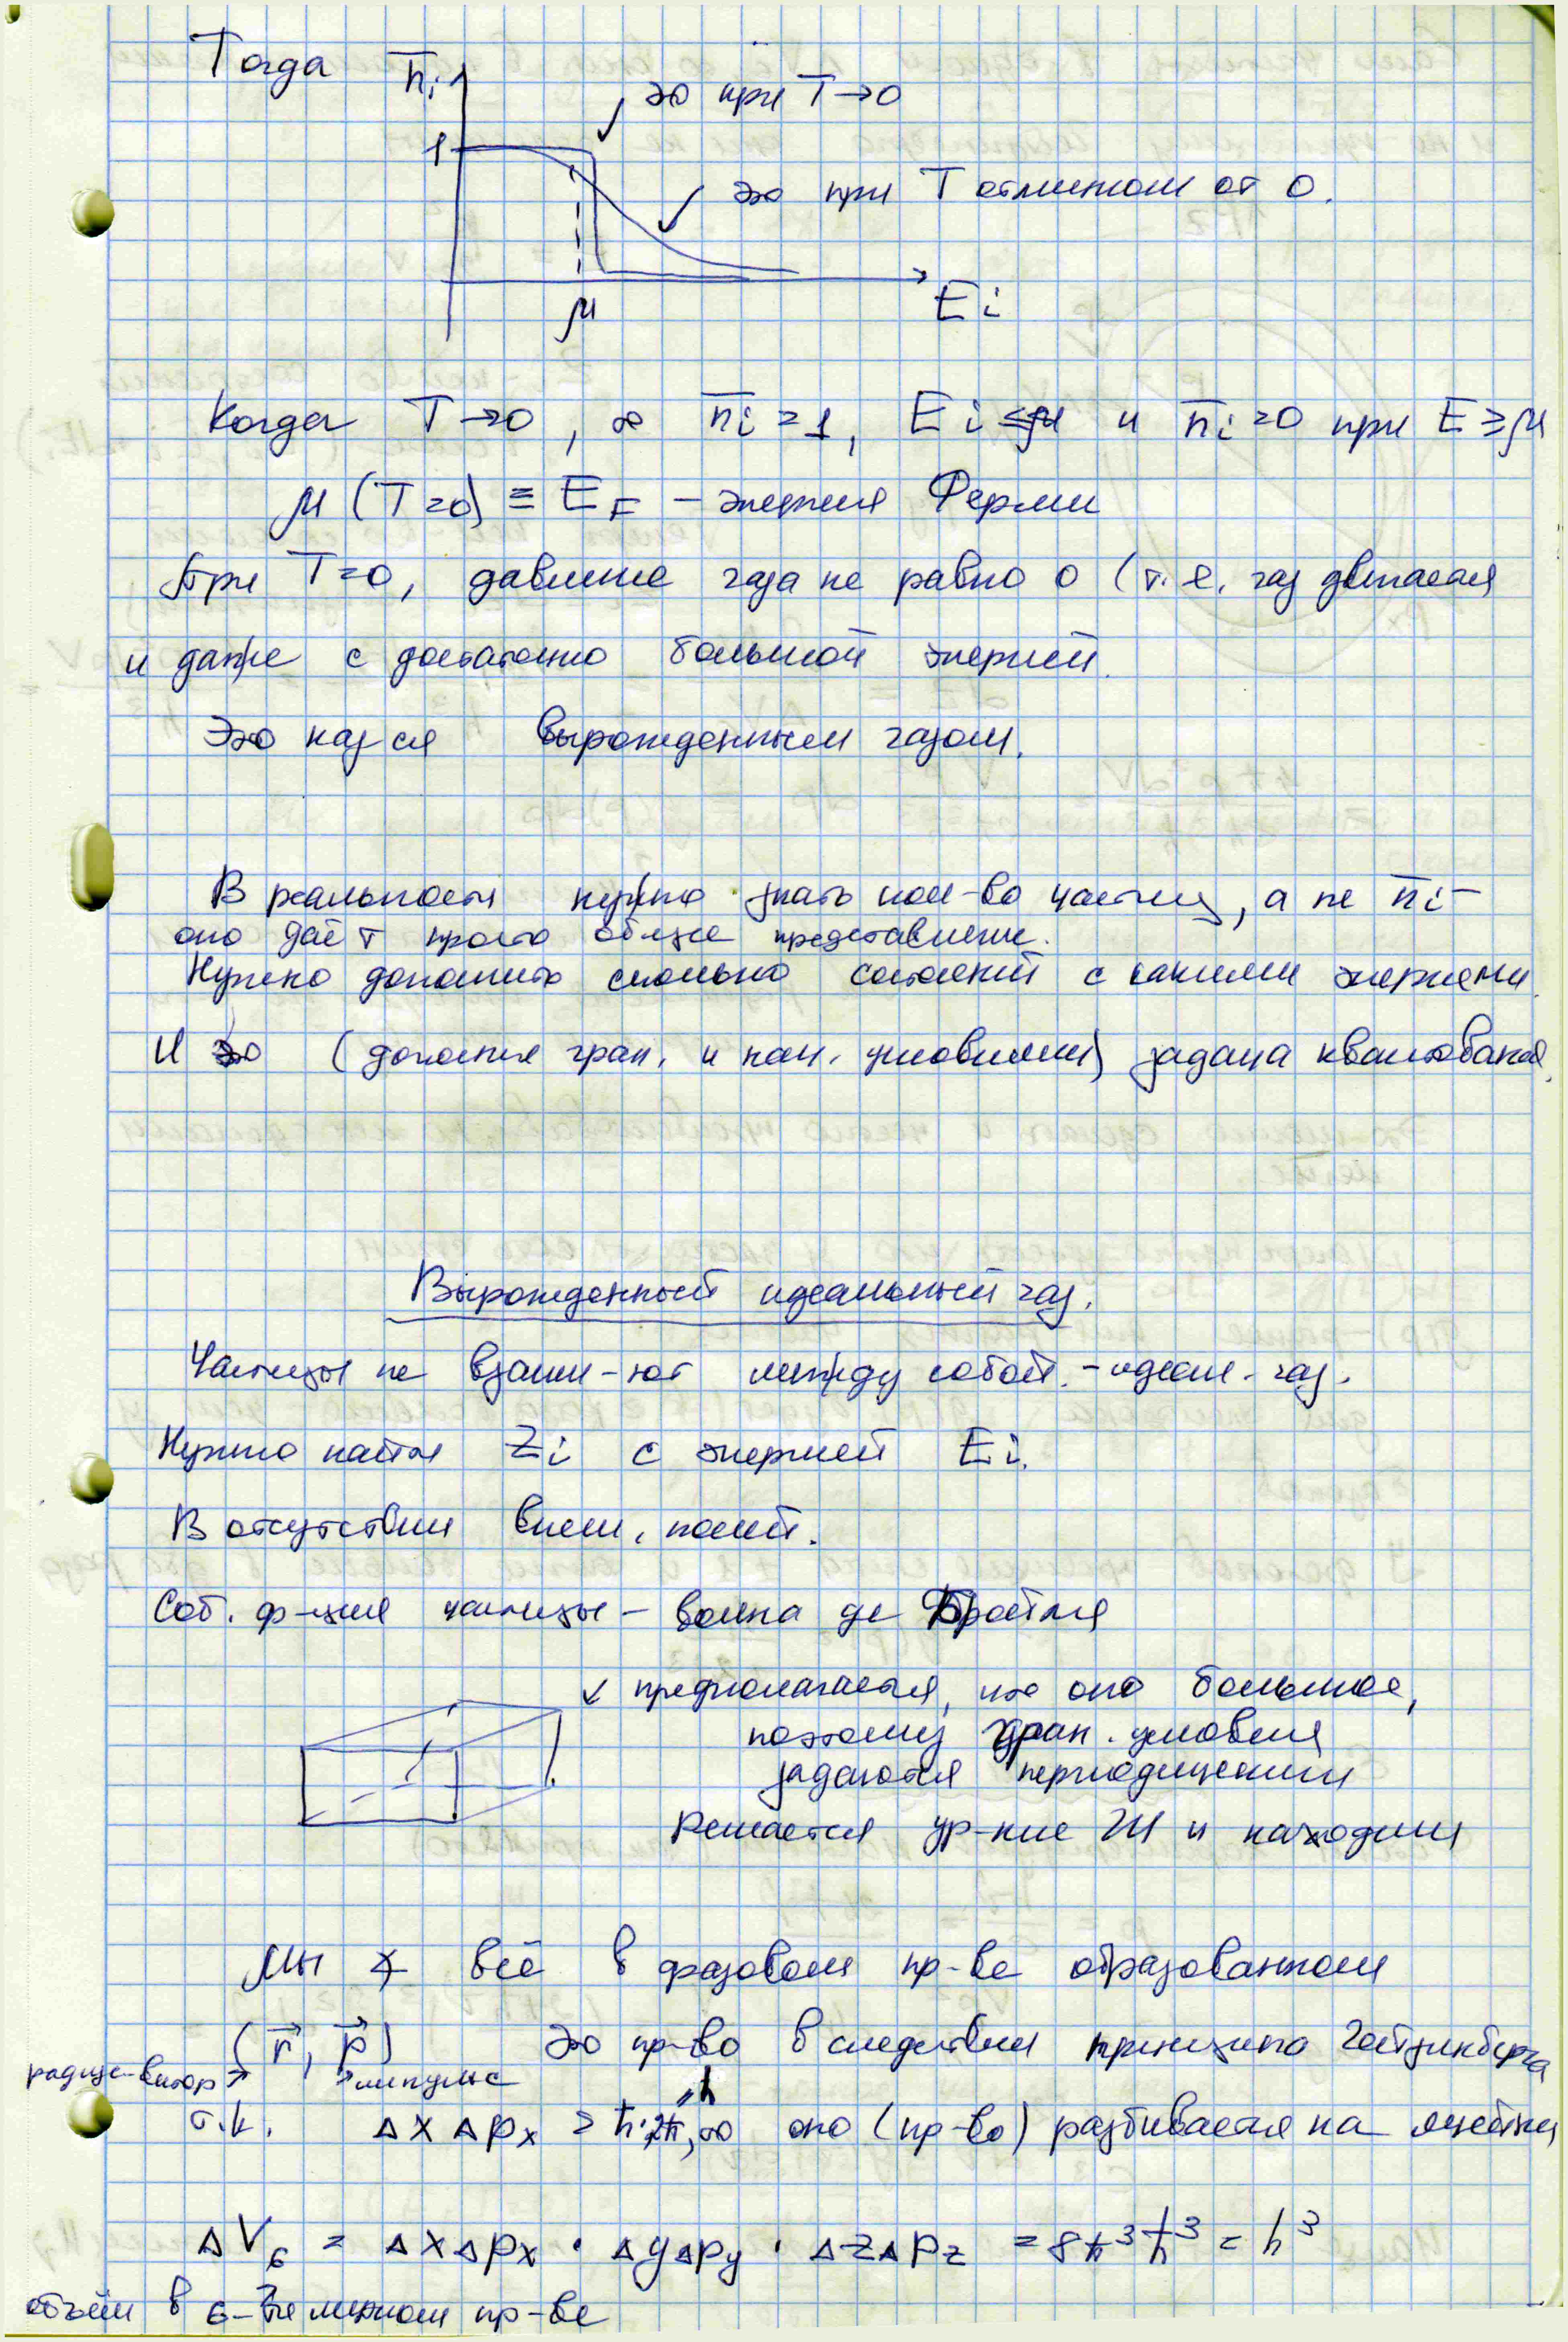
\includegraphics[max size={\textwidth}{0.995\textheight}]{jpg/26.jpg}%
\newpage%
%
%
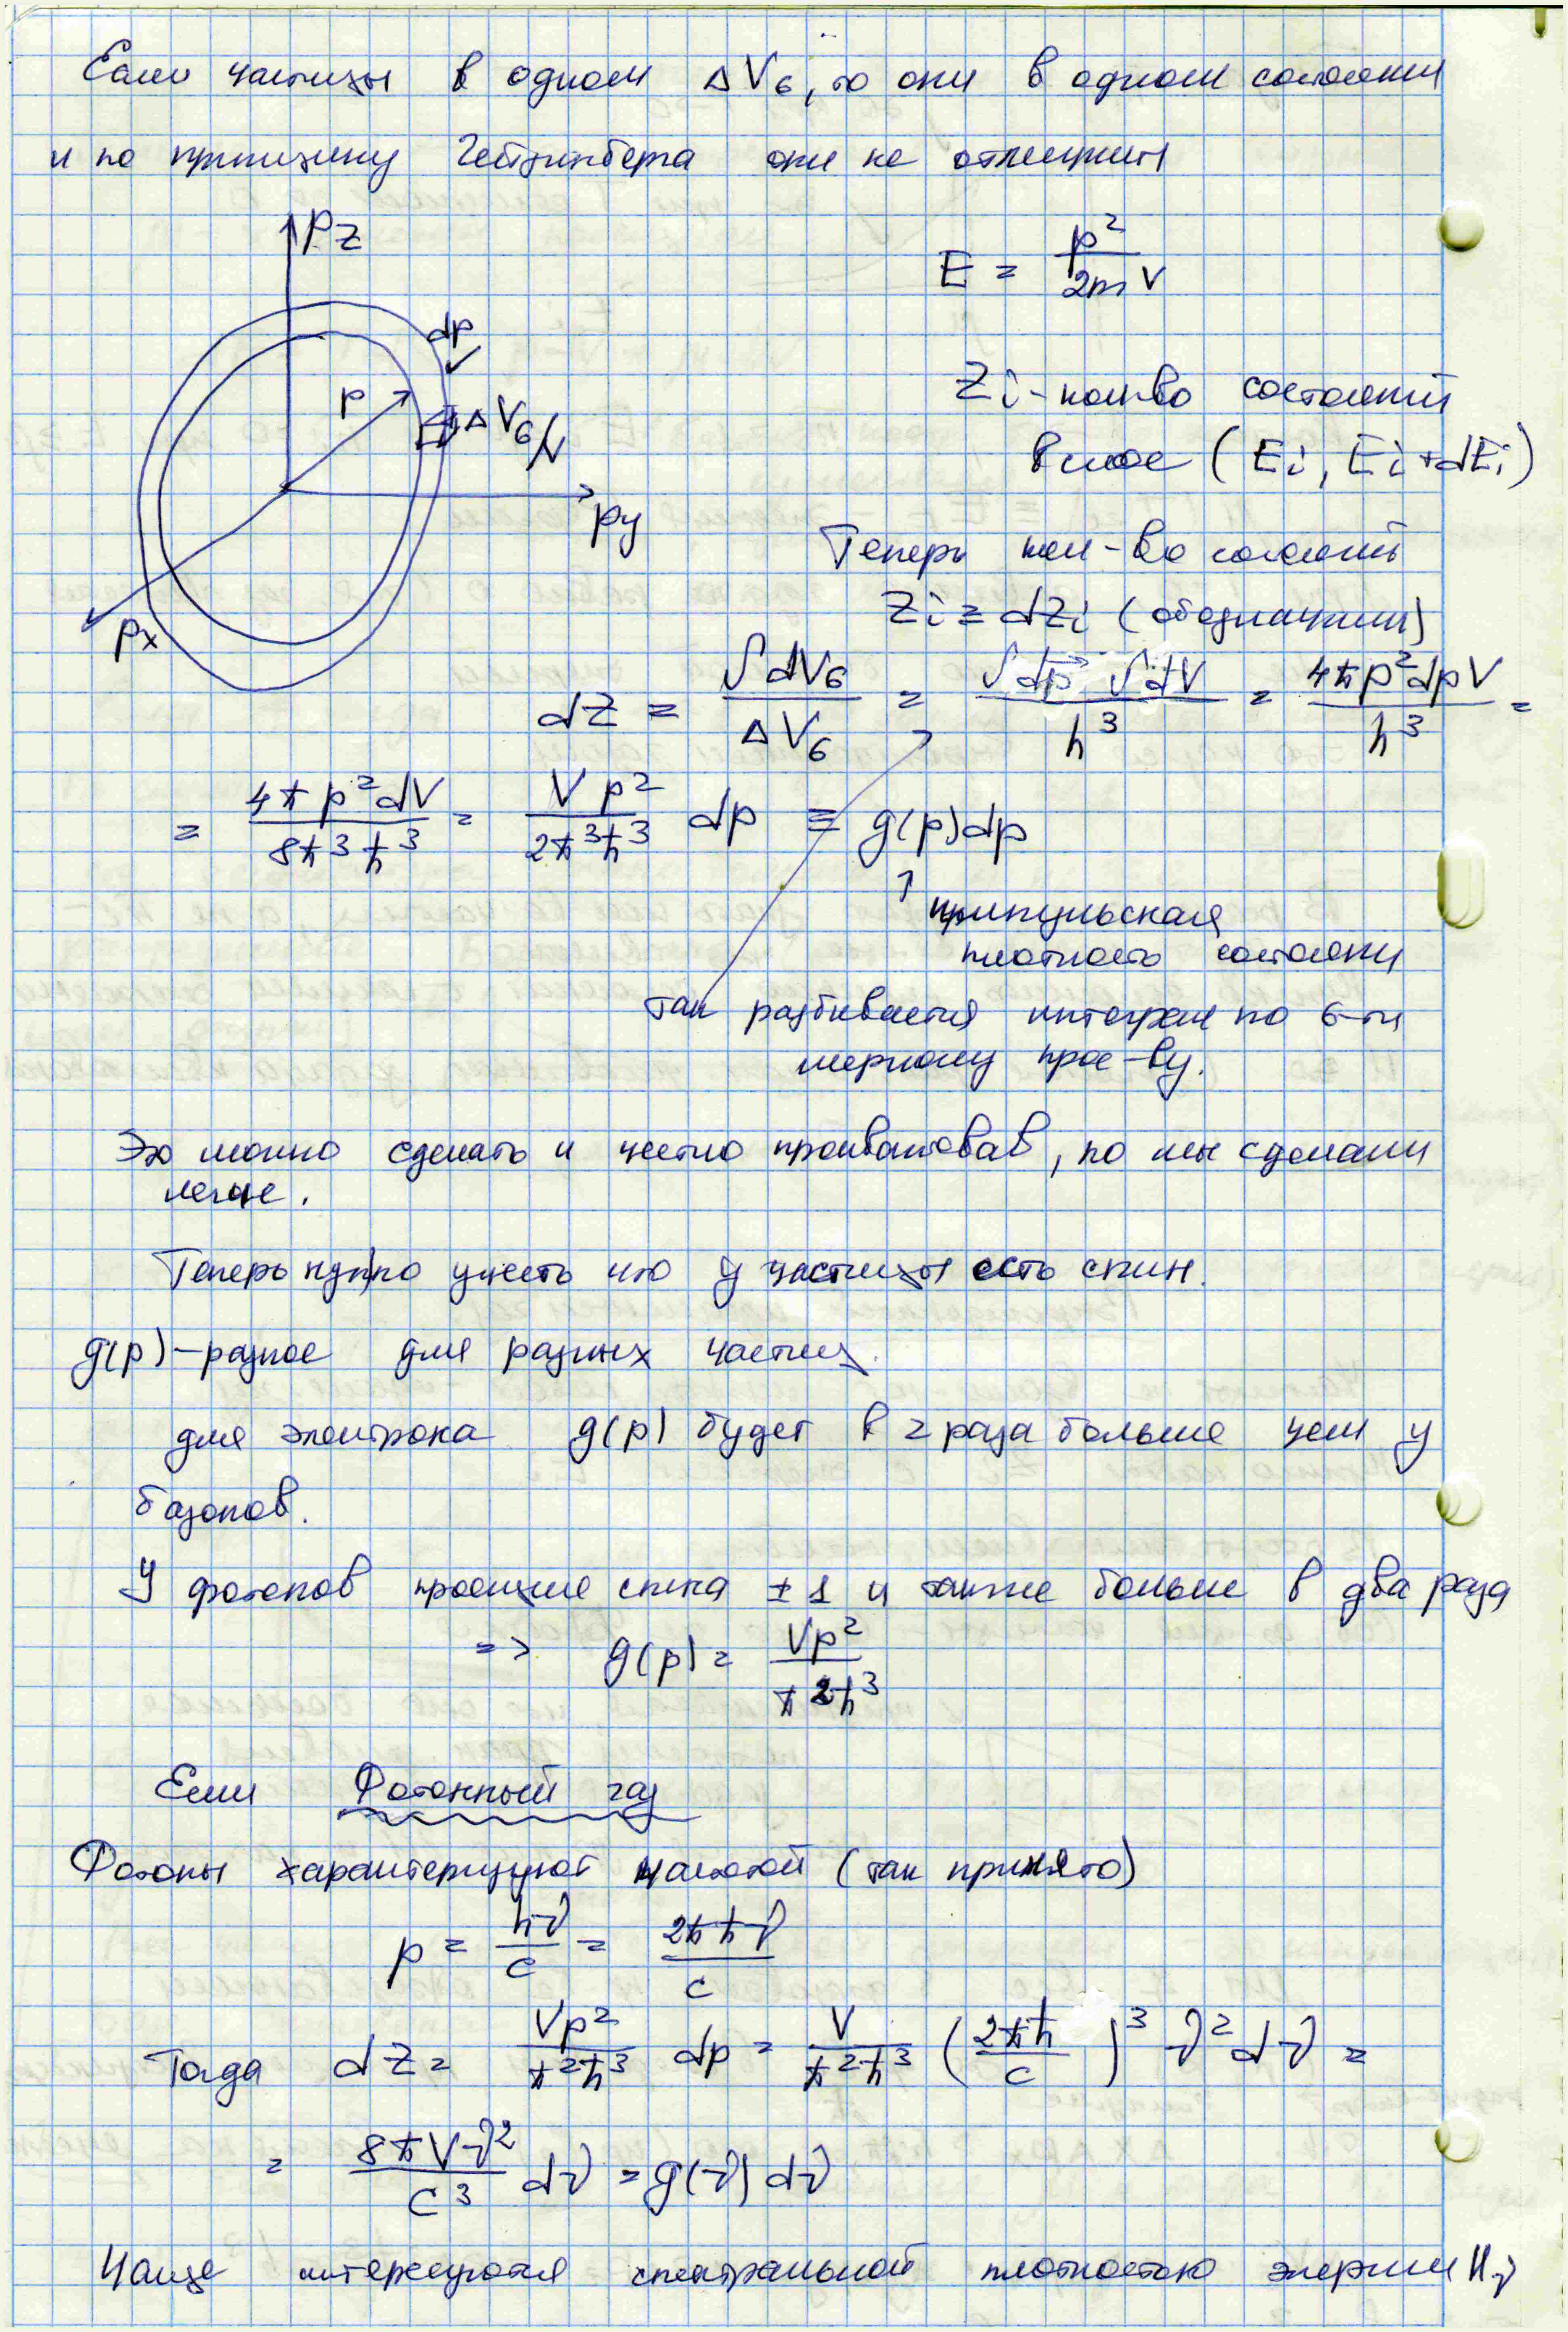
\includegraphics[max size={\textwidth}{0.995\textheight}]{jpg/27.jpg}%
\newpage%
%
%
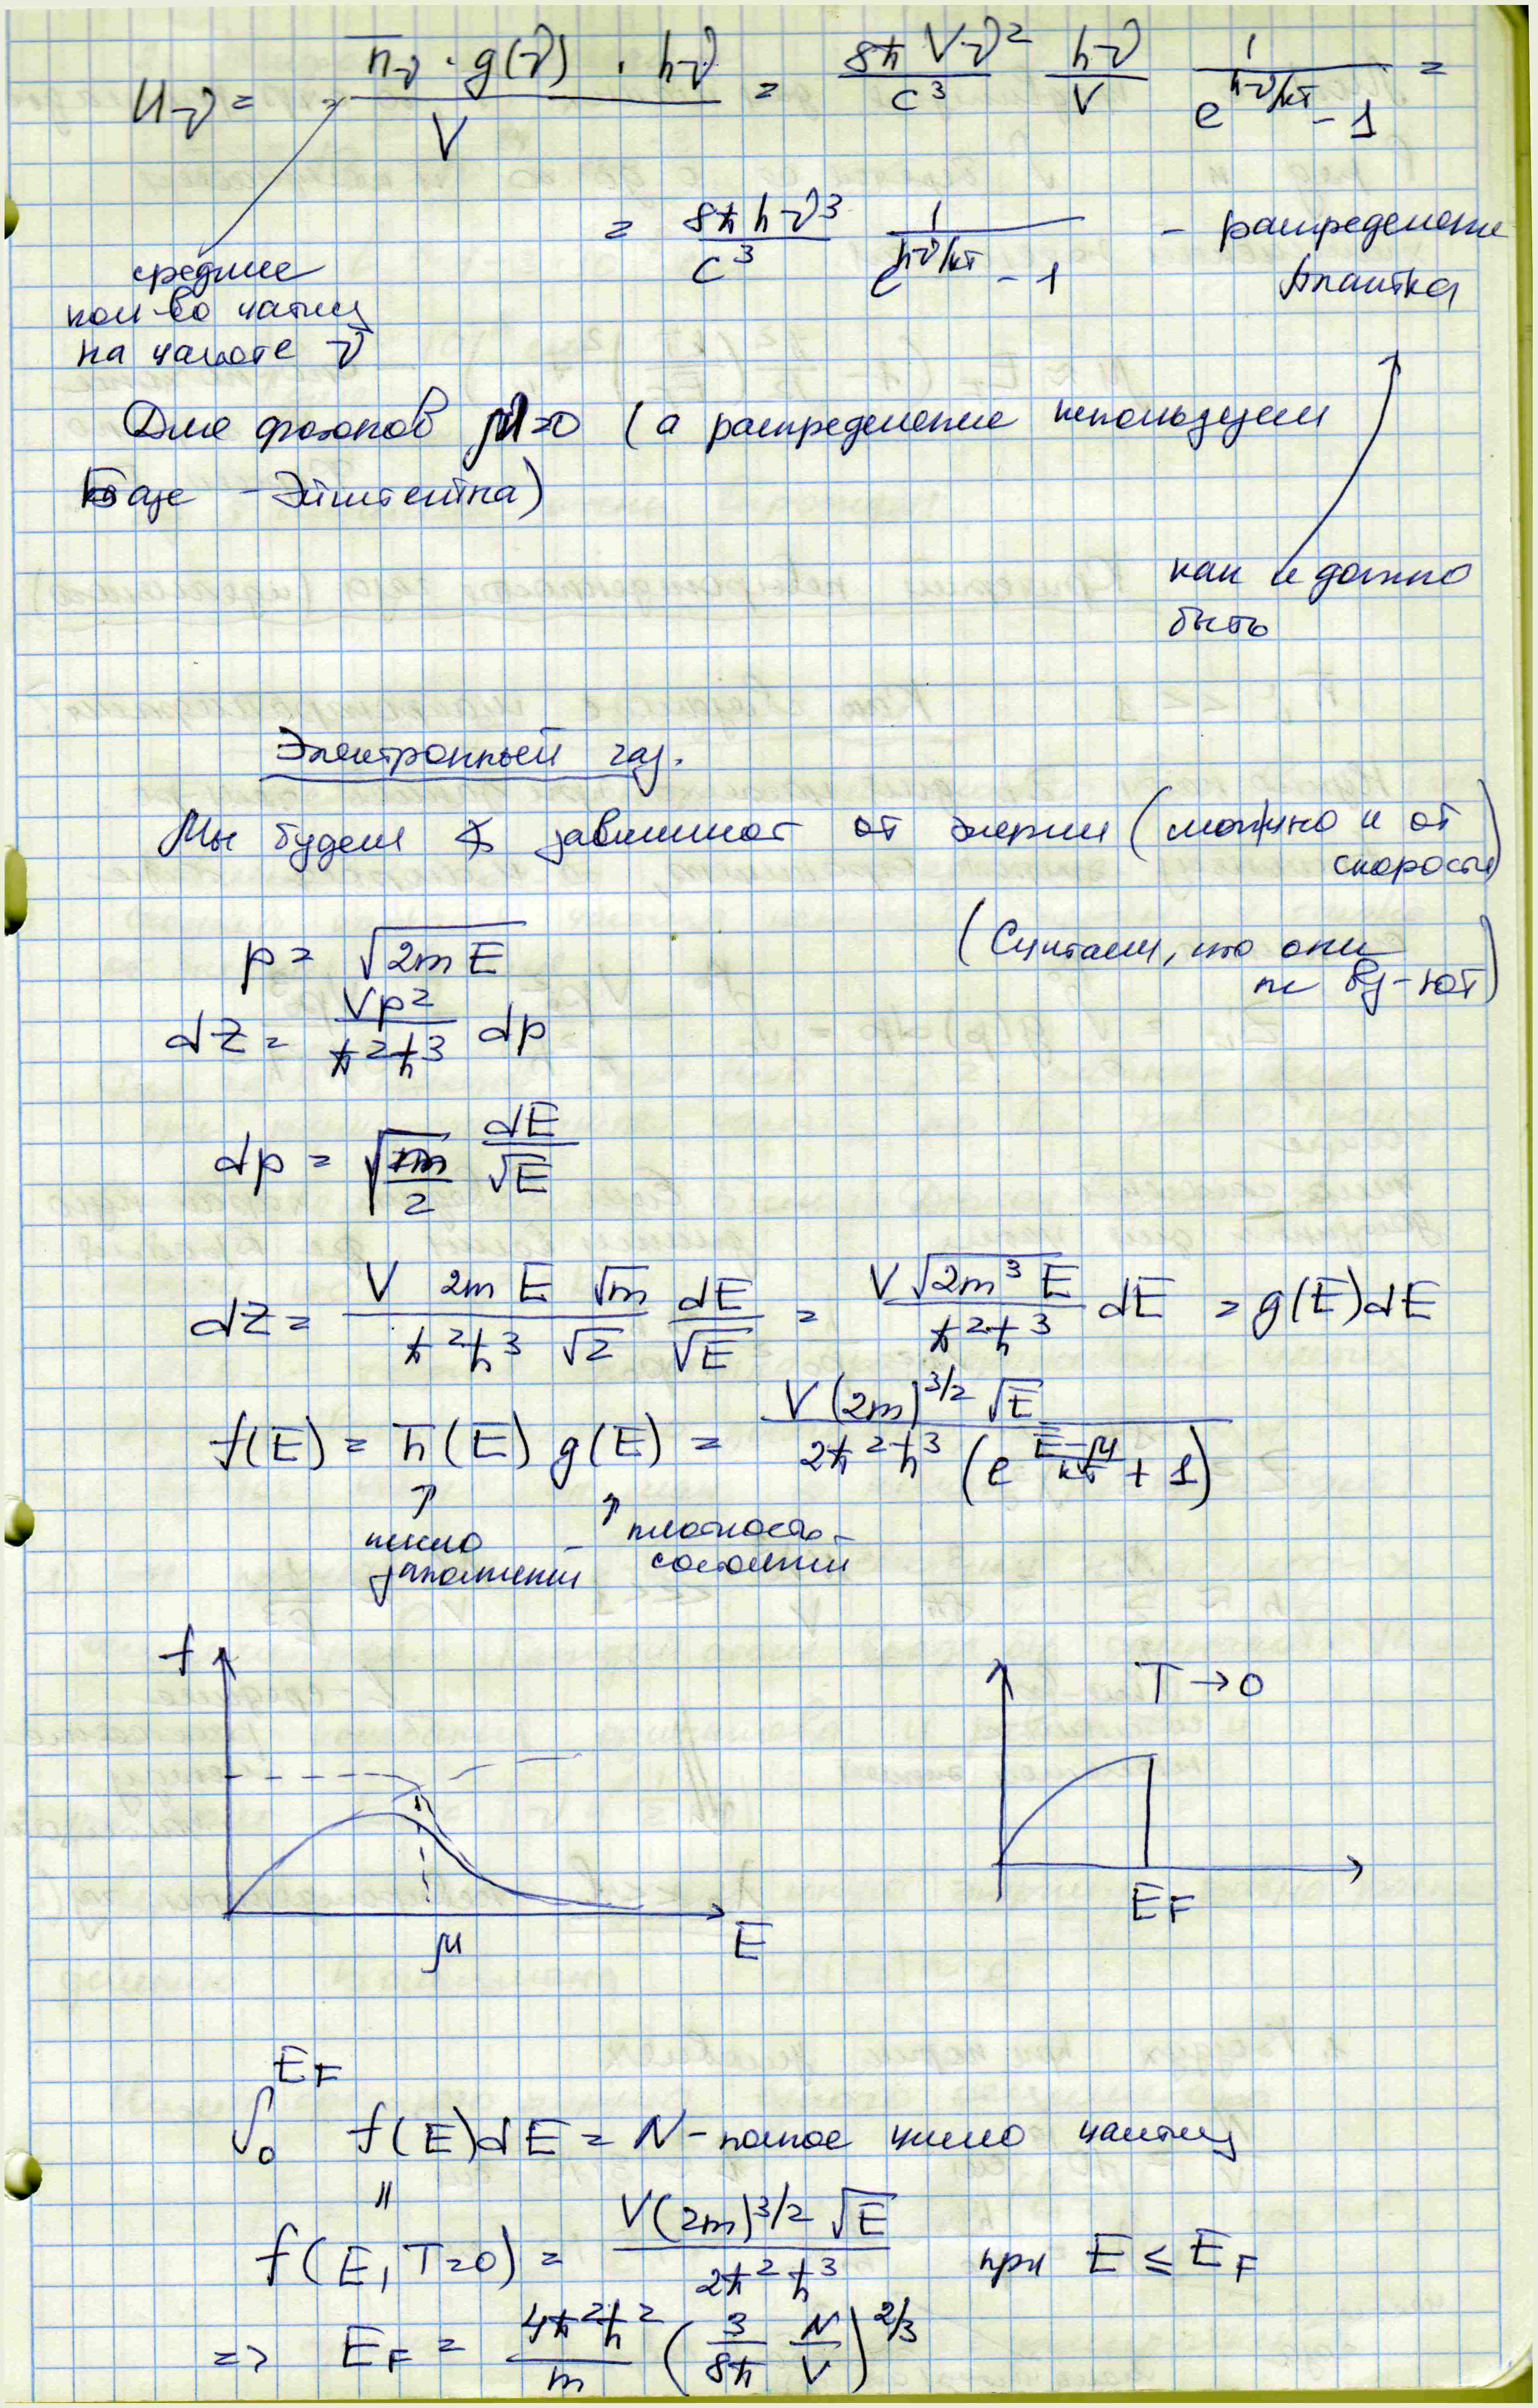
\includegraphics[max size={\textwidth}{0.995\textheight}]{jpg/28.jpg}%
\newpage%
%
\phantomsection\addcontentsline{toc}{subsubsection}{Критерий невырожденности ИГ}%
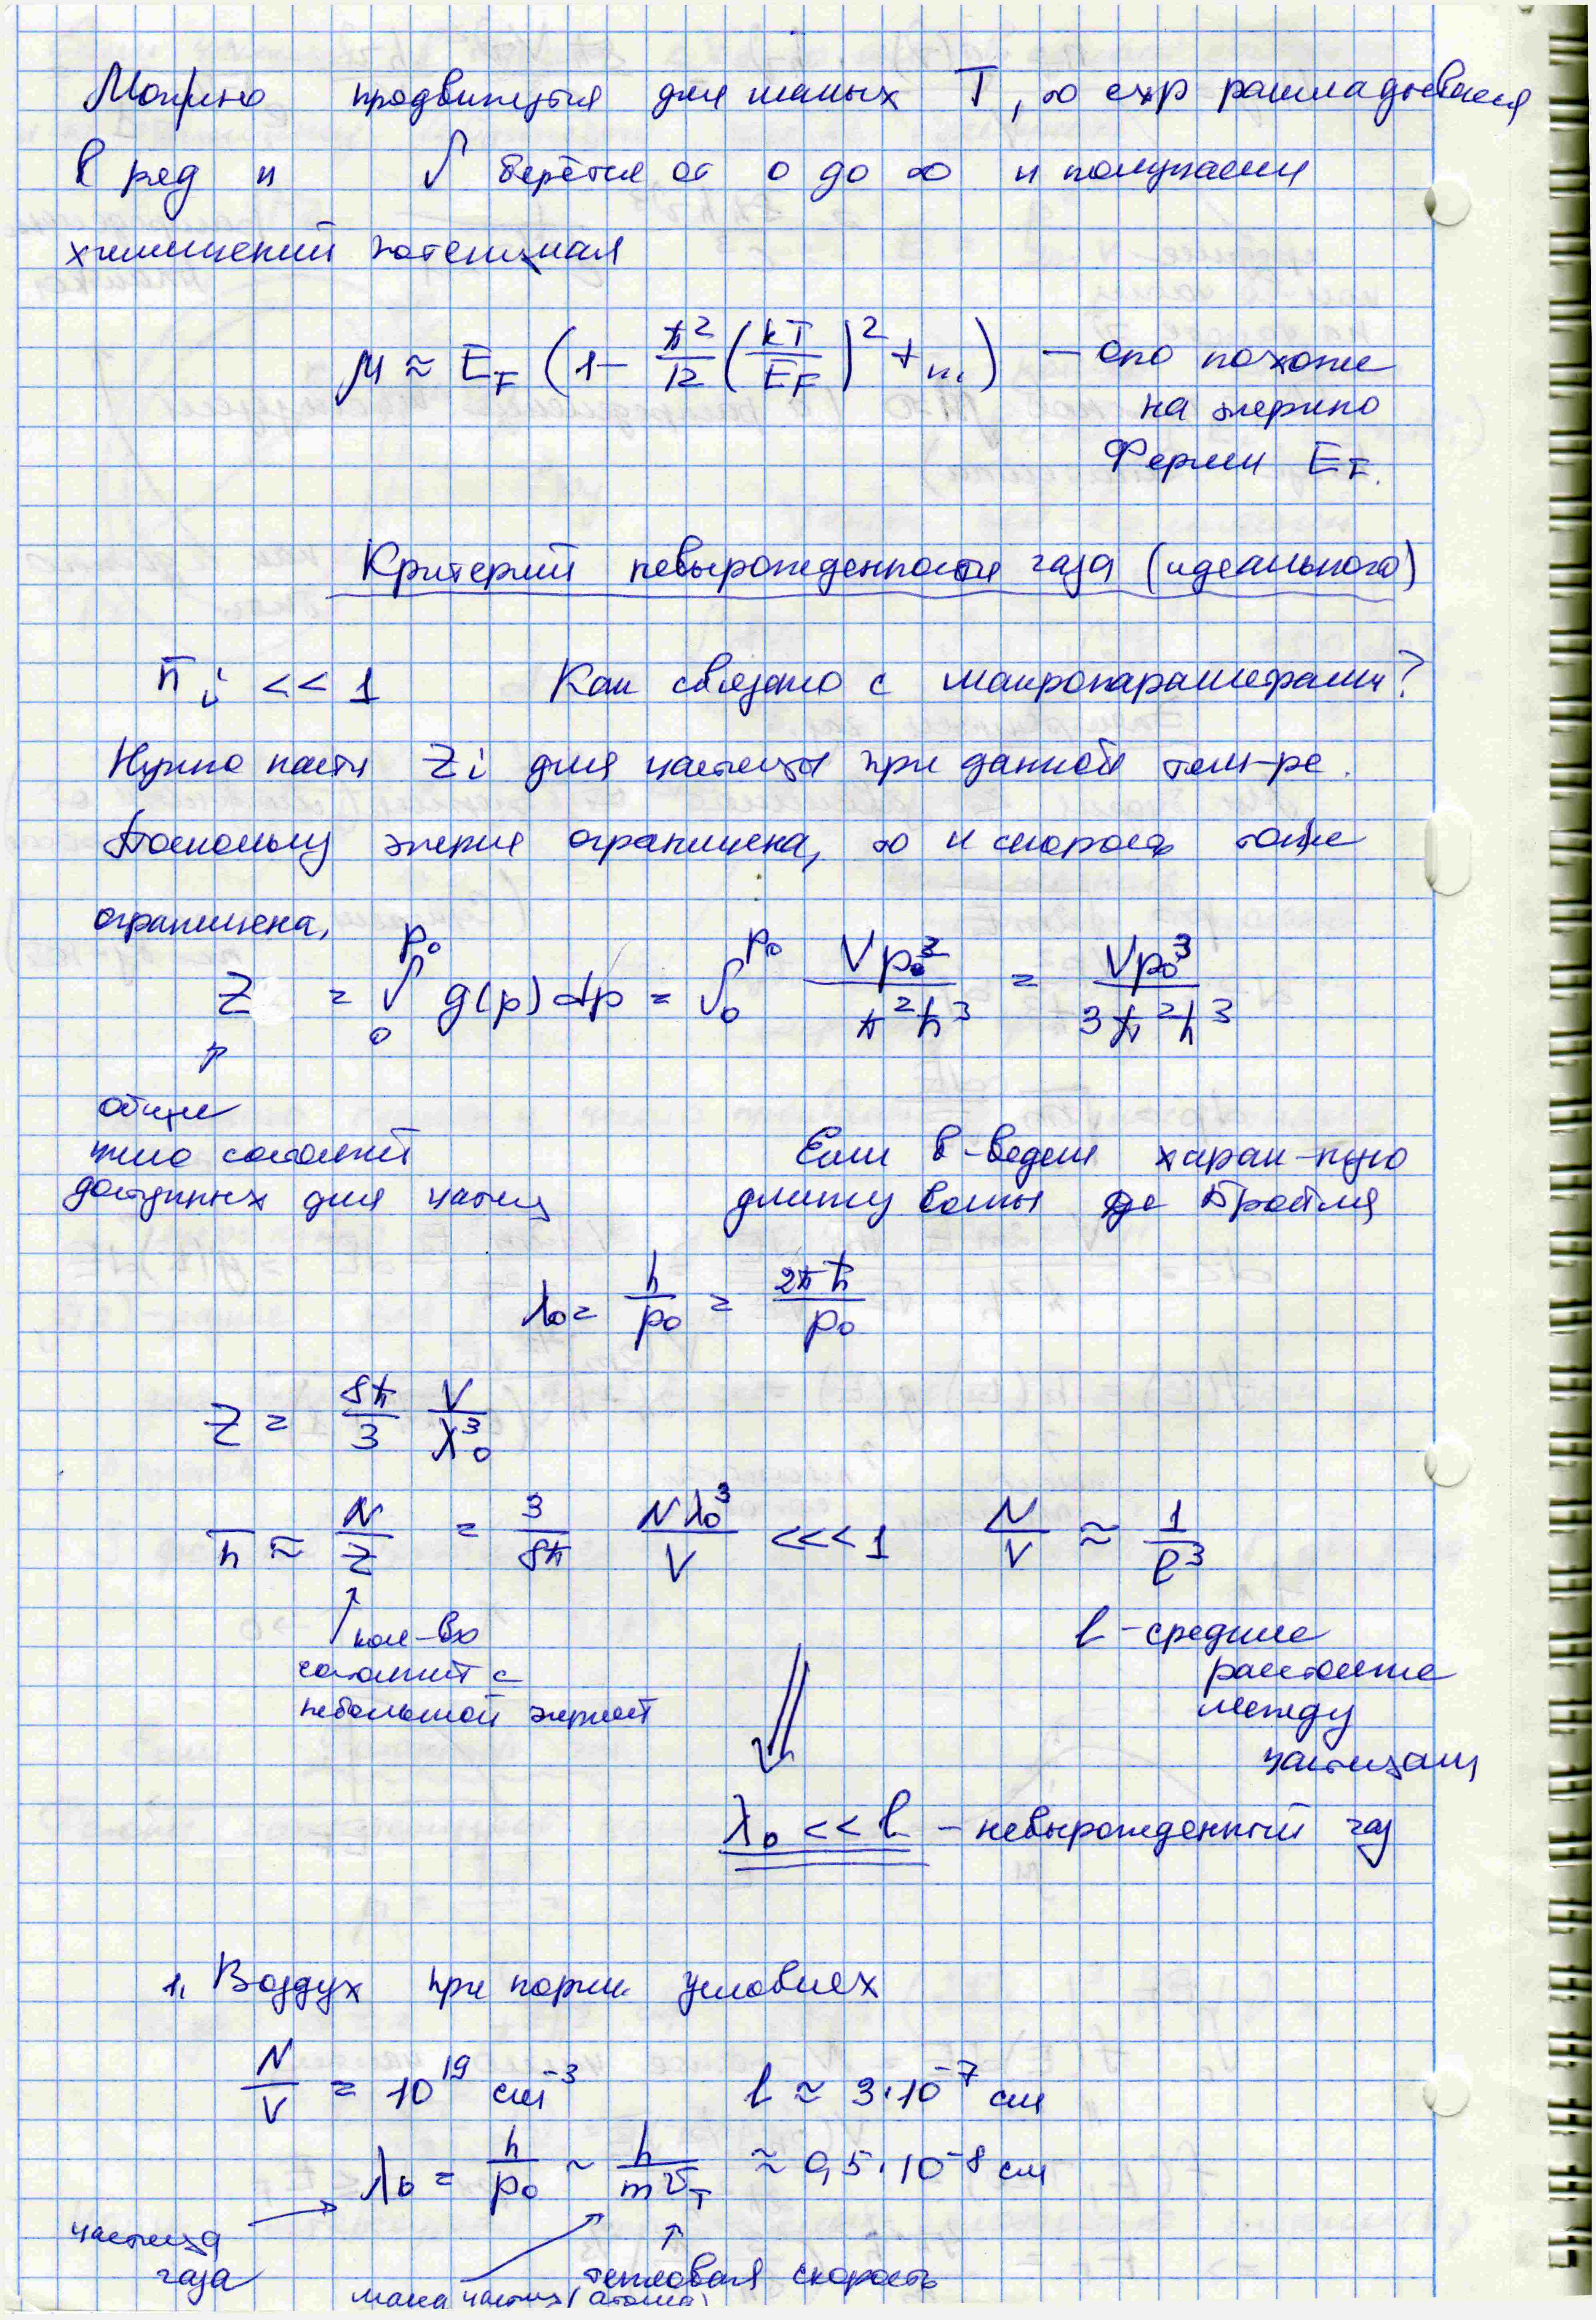
\includegraphics[max size={\textwidth}{0.995\textheight}]{jpg/29.jpg}%
\newpage%
%
\phantomsection\addcontentsline{toc}{subsection}{Теплоемкость твердых тел}%
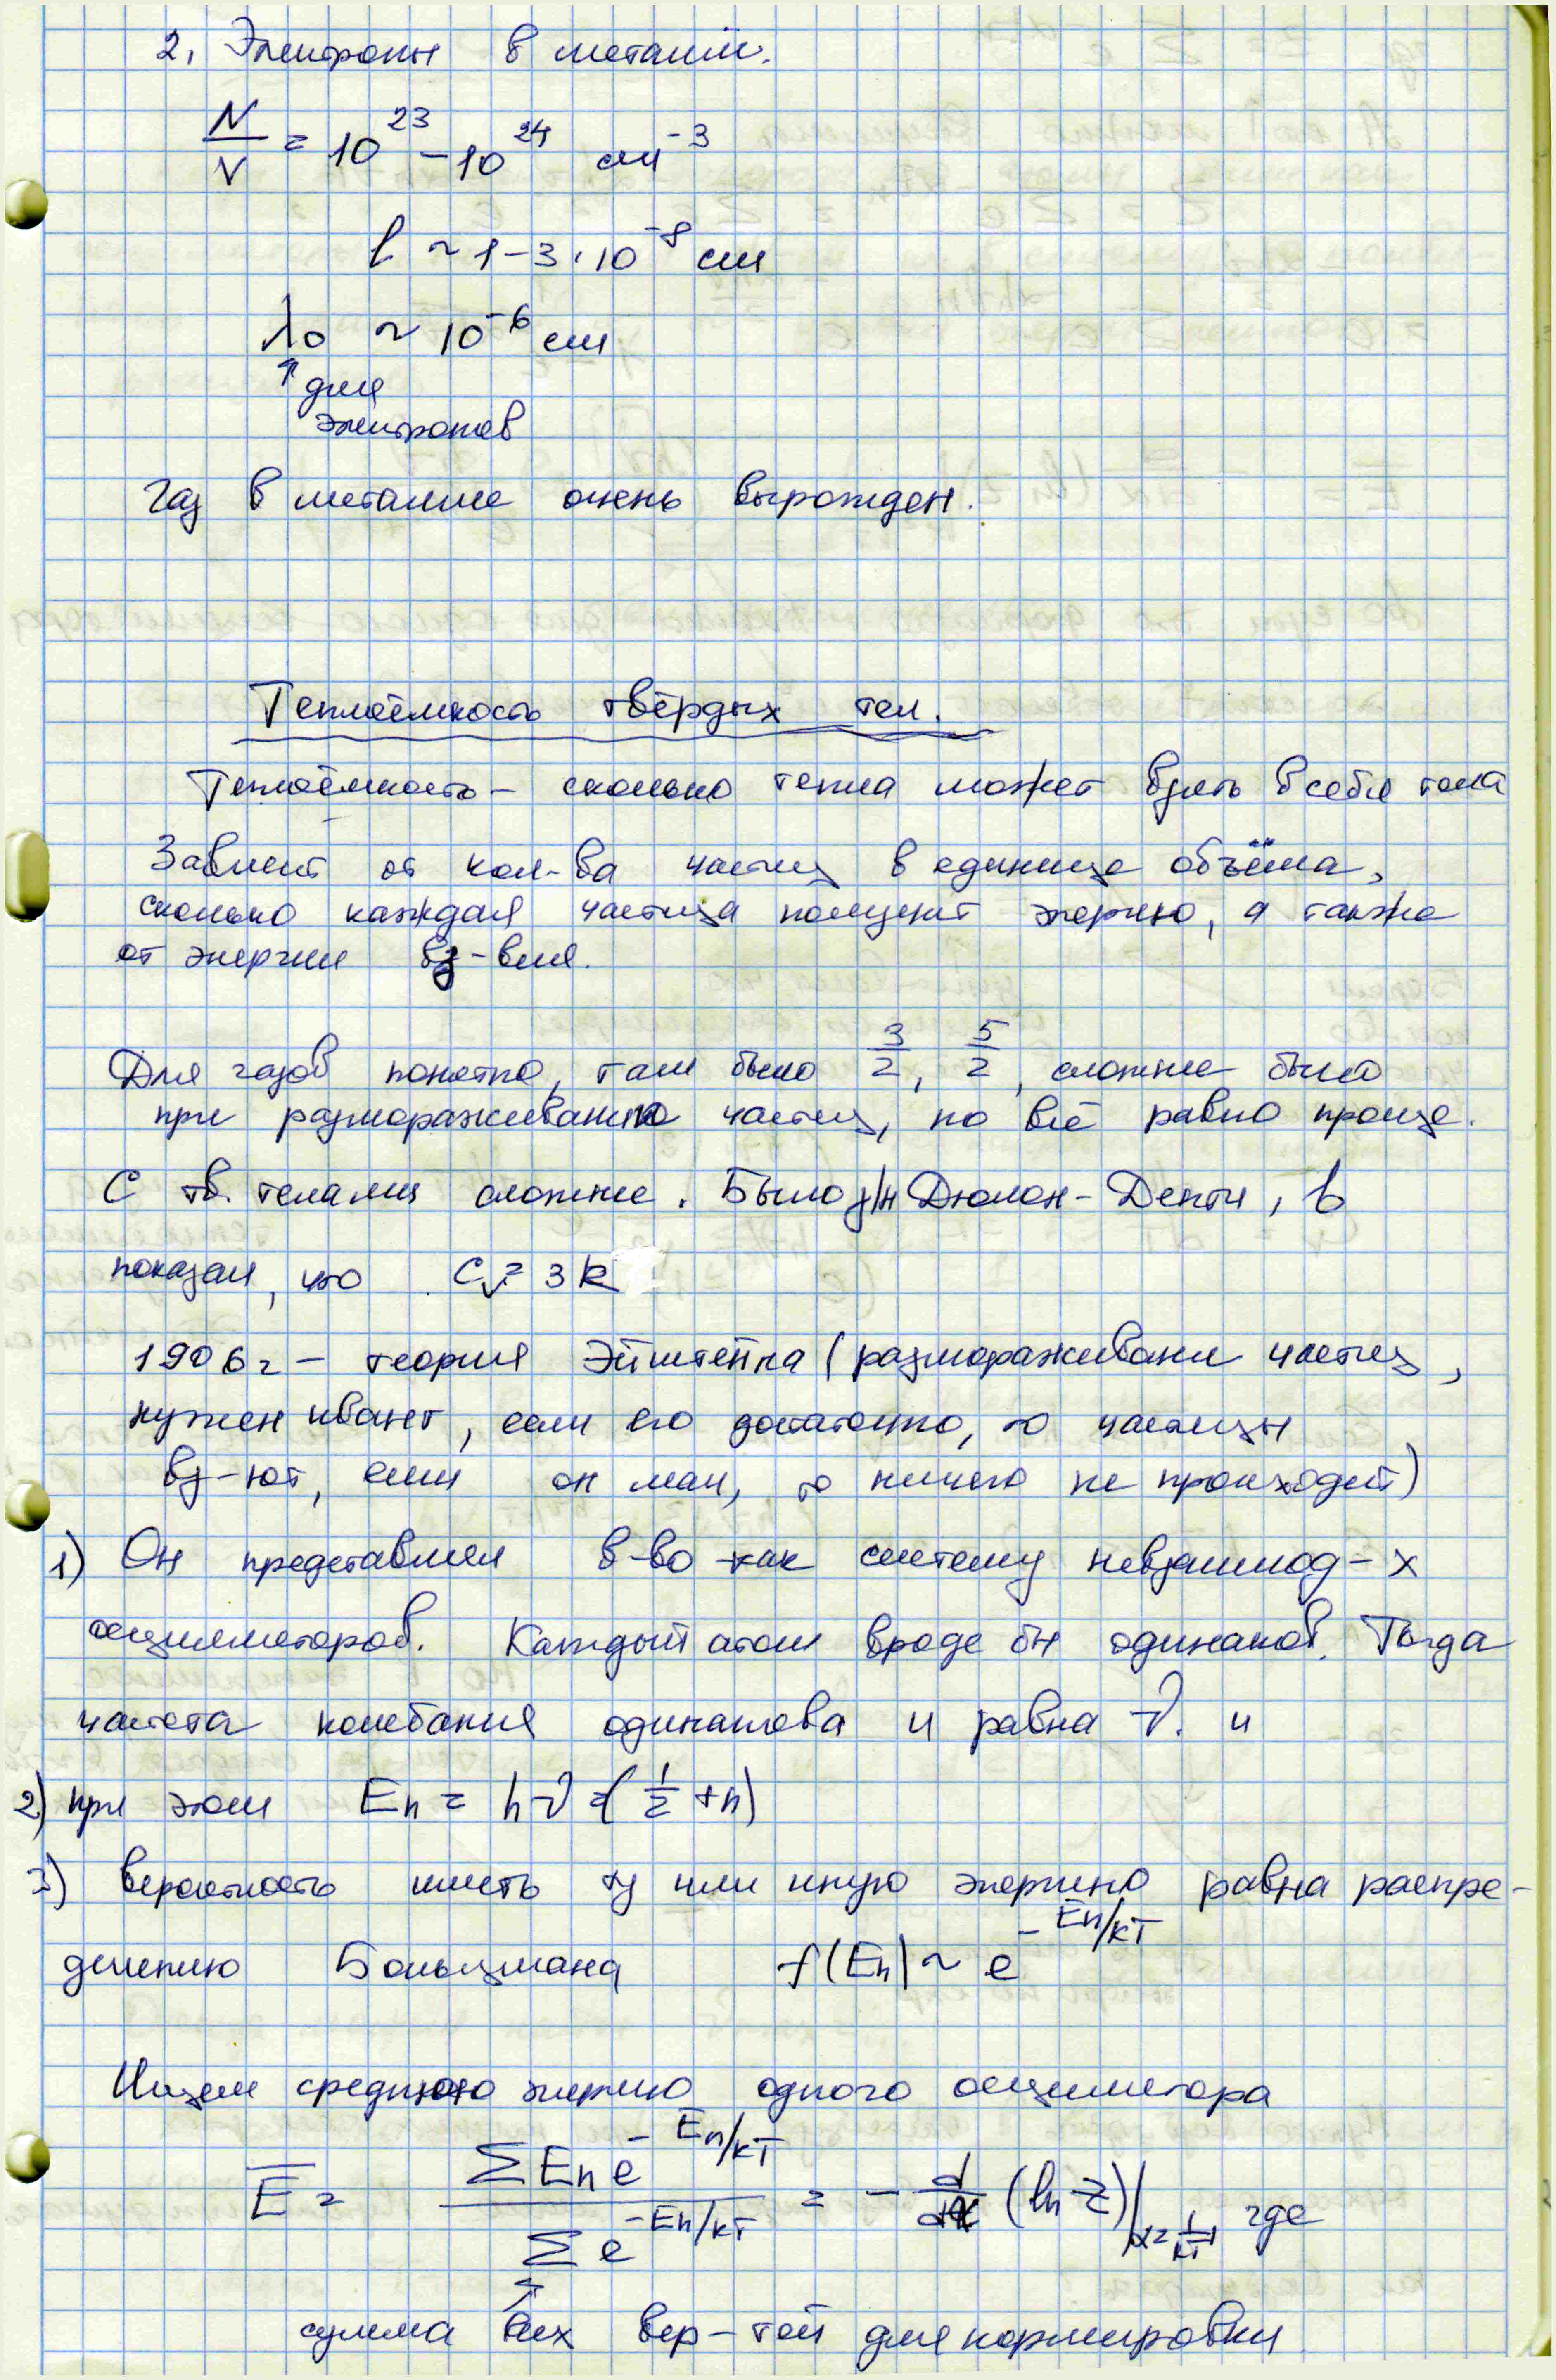
\includegraphics[max size={\textwidth}{0.995\textheight}]{jpg/30.jpg}%
\newpage%
%
%
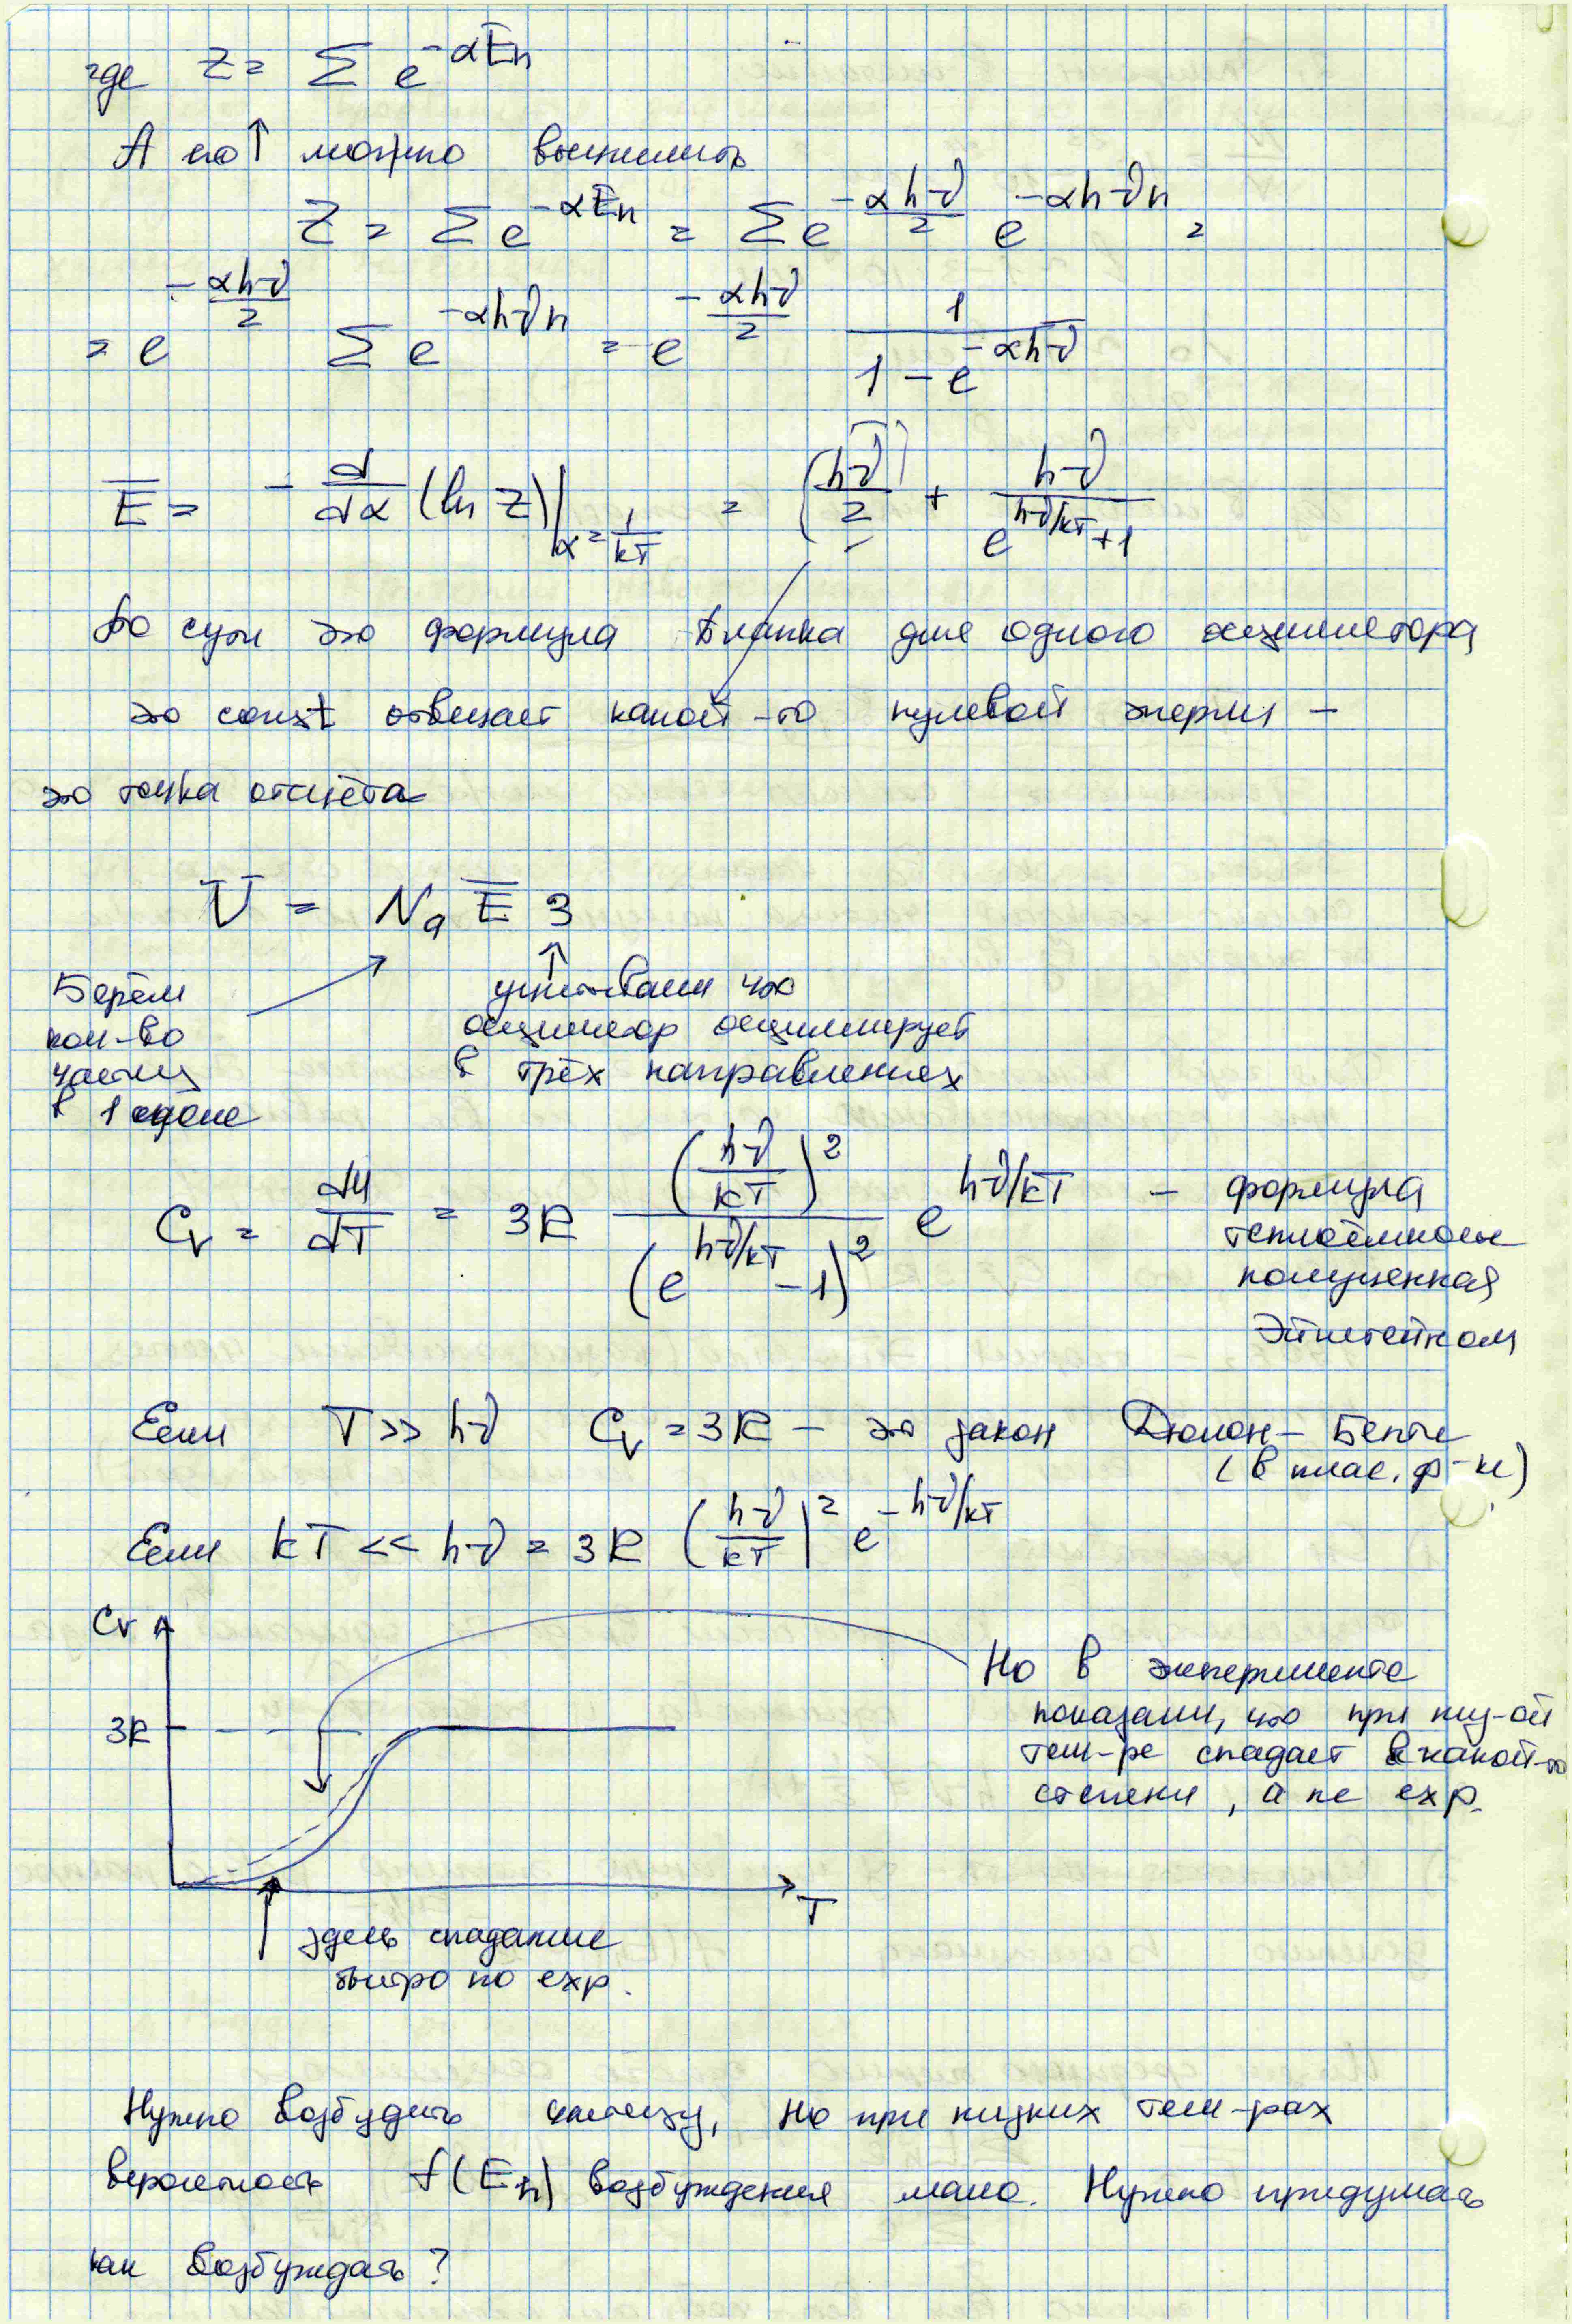
\includegraphics[max size={\textwidth}{0.995\textheight}]{jpg/31.jpg}%
\newpage%
%
%
\phantomsection\addcontentsline{toc}{subsubsection}{Теория Дебая}%
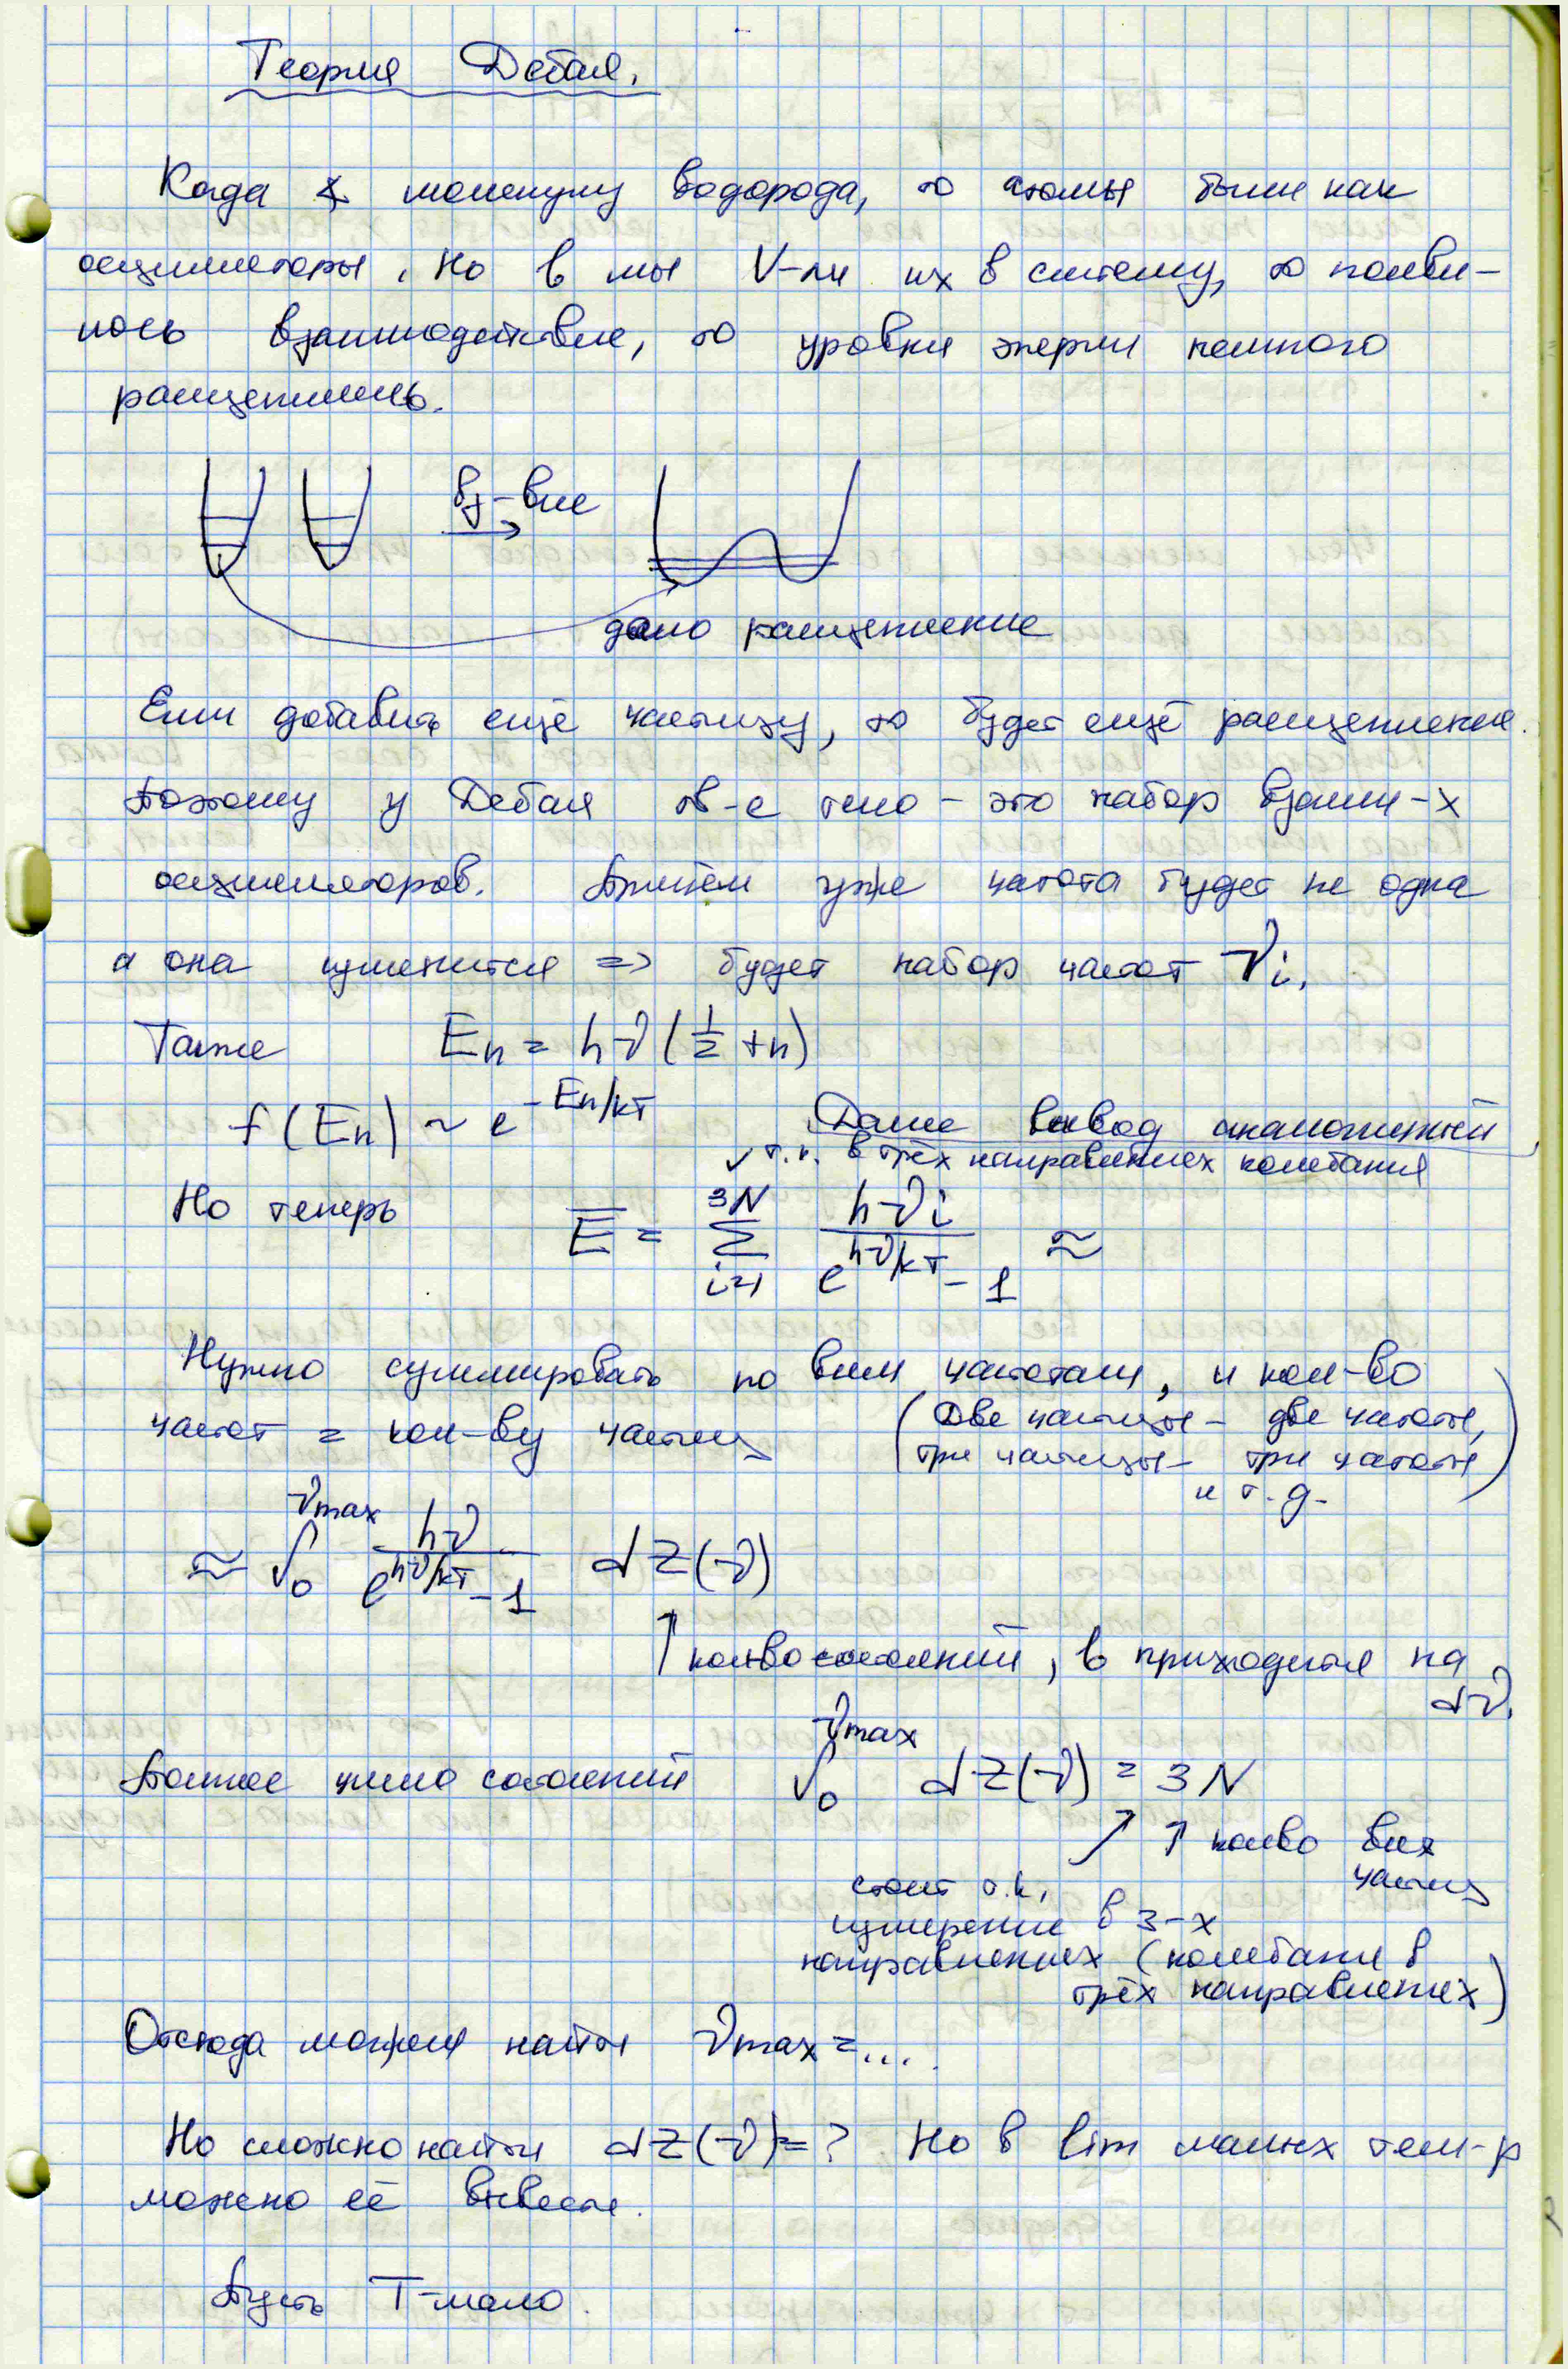
\includegraphics[max size={\textwidth}{0.995\textheight}]{jpg/32.jpg}%
\newpage%
%
%
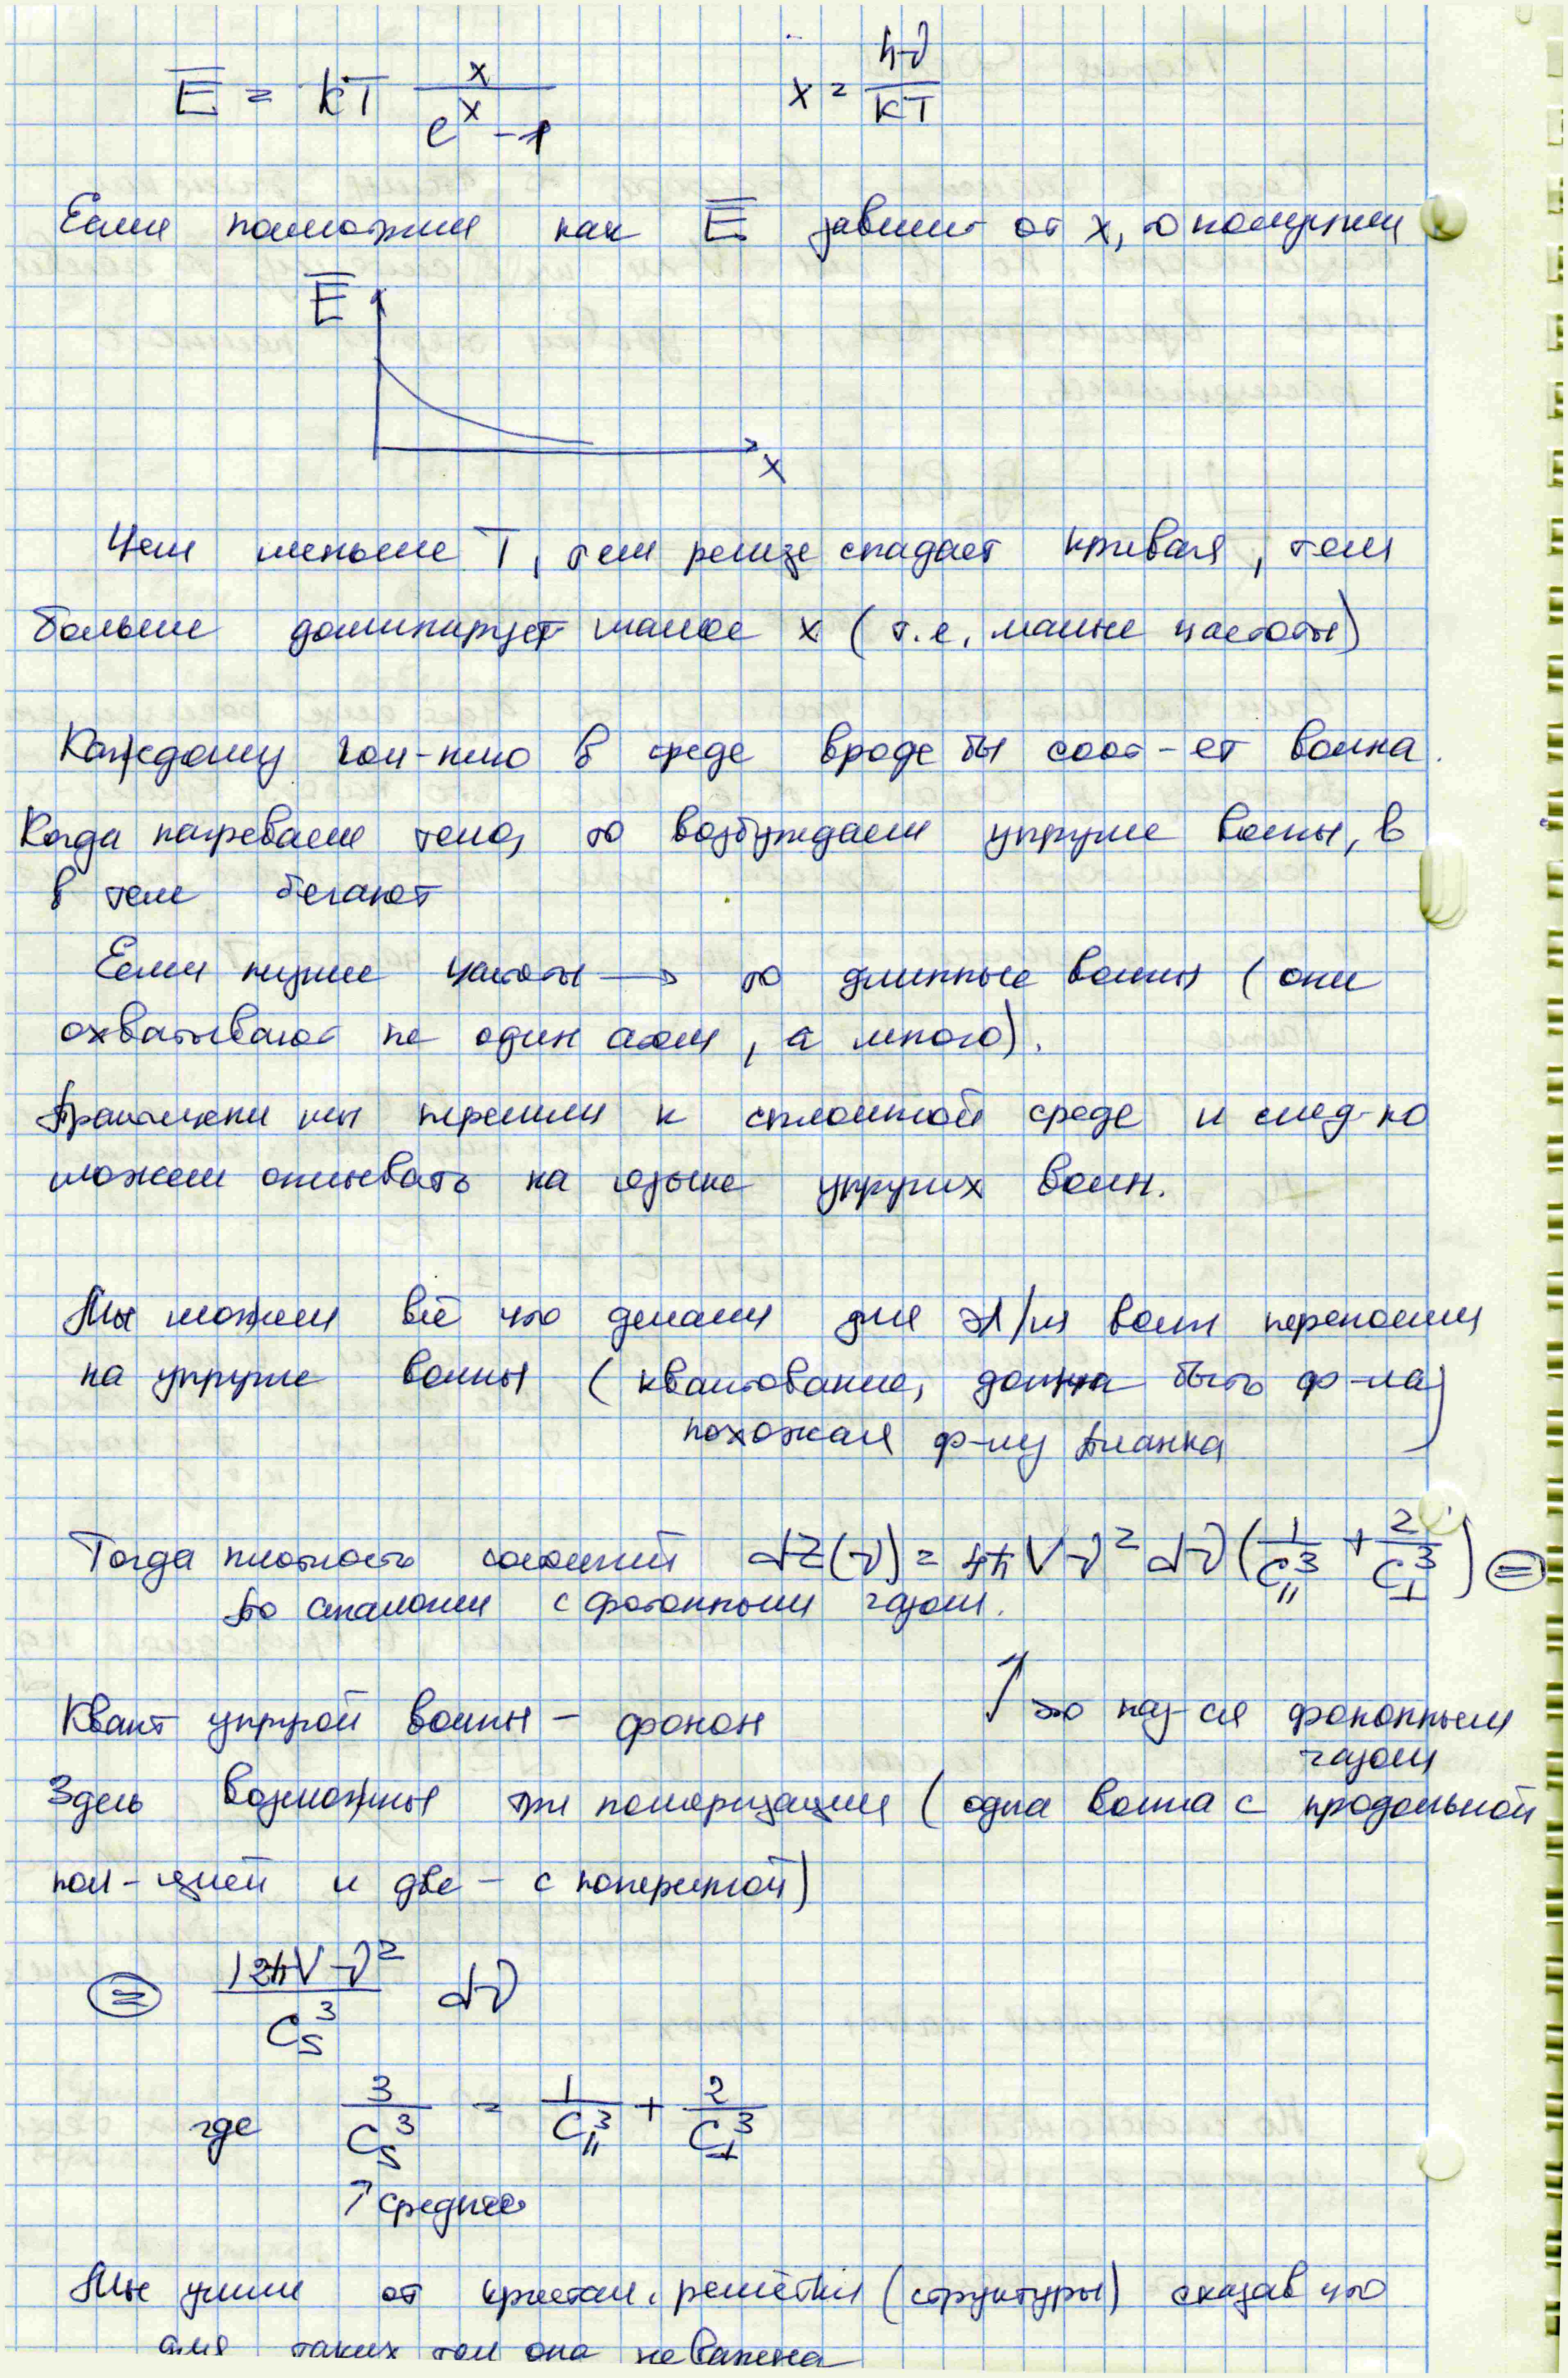
\includegraphics[max size={\textwidth}{0.995\textheight}]{jpg/33.jpg}%
\newpage%
%
%
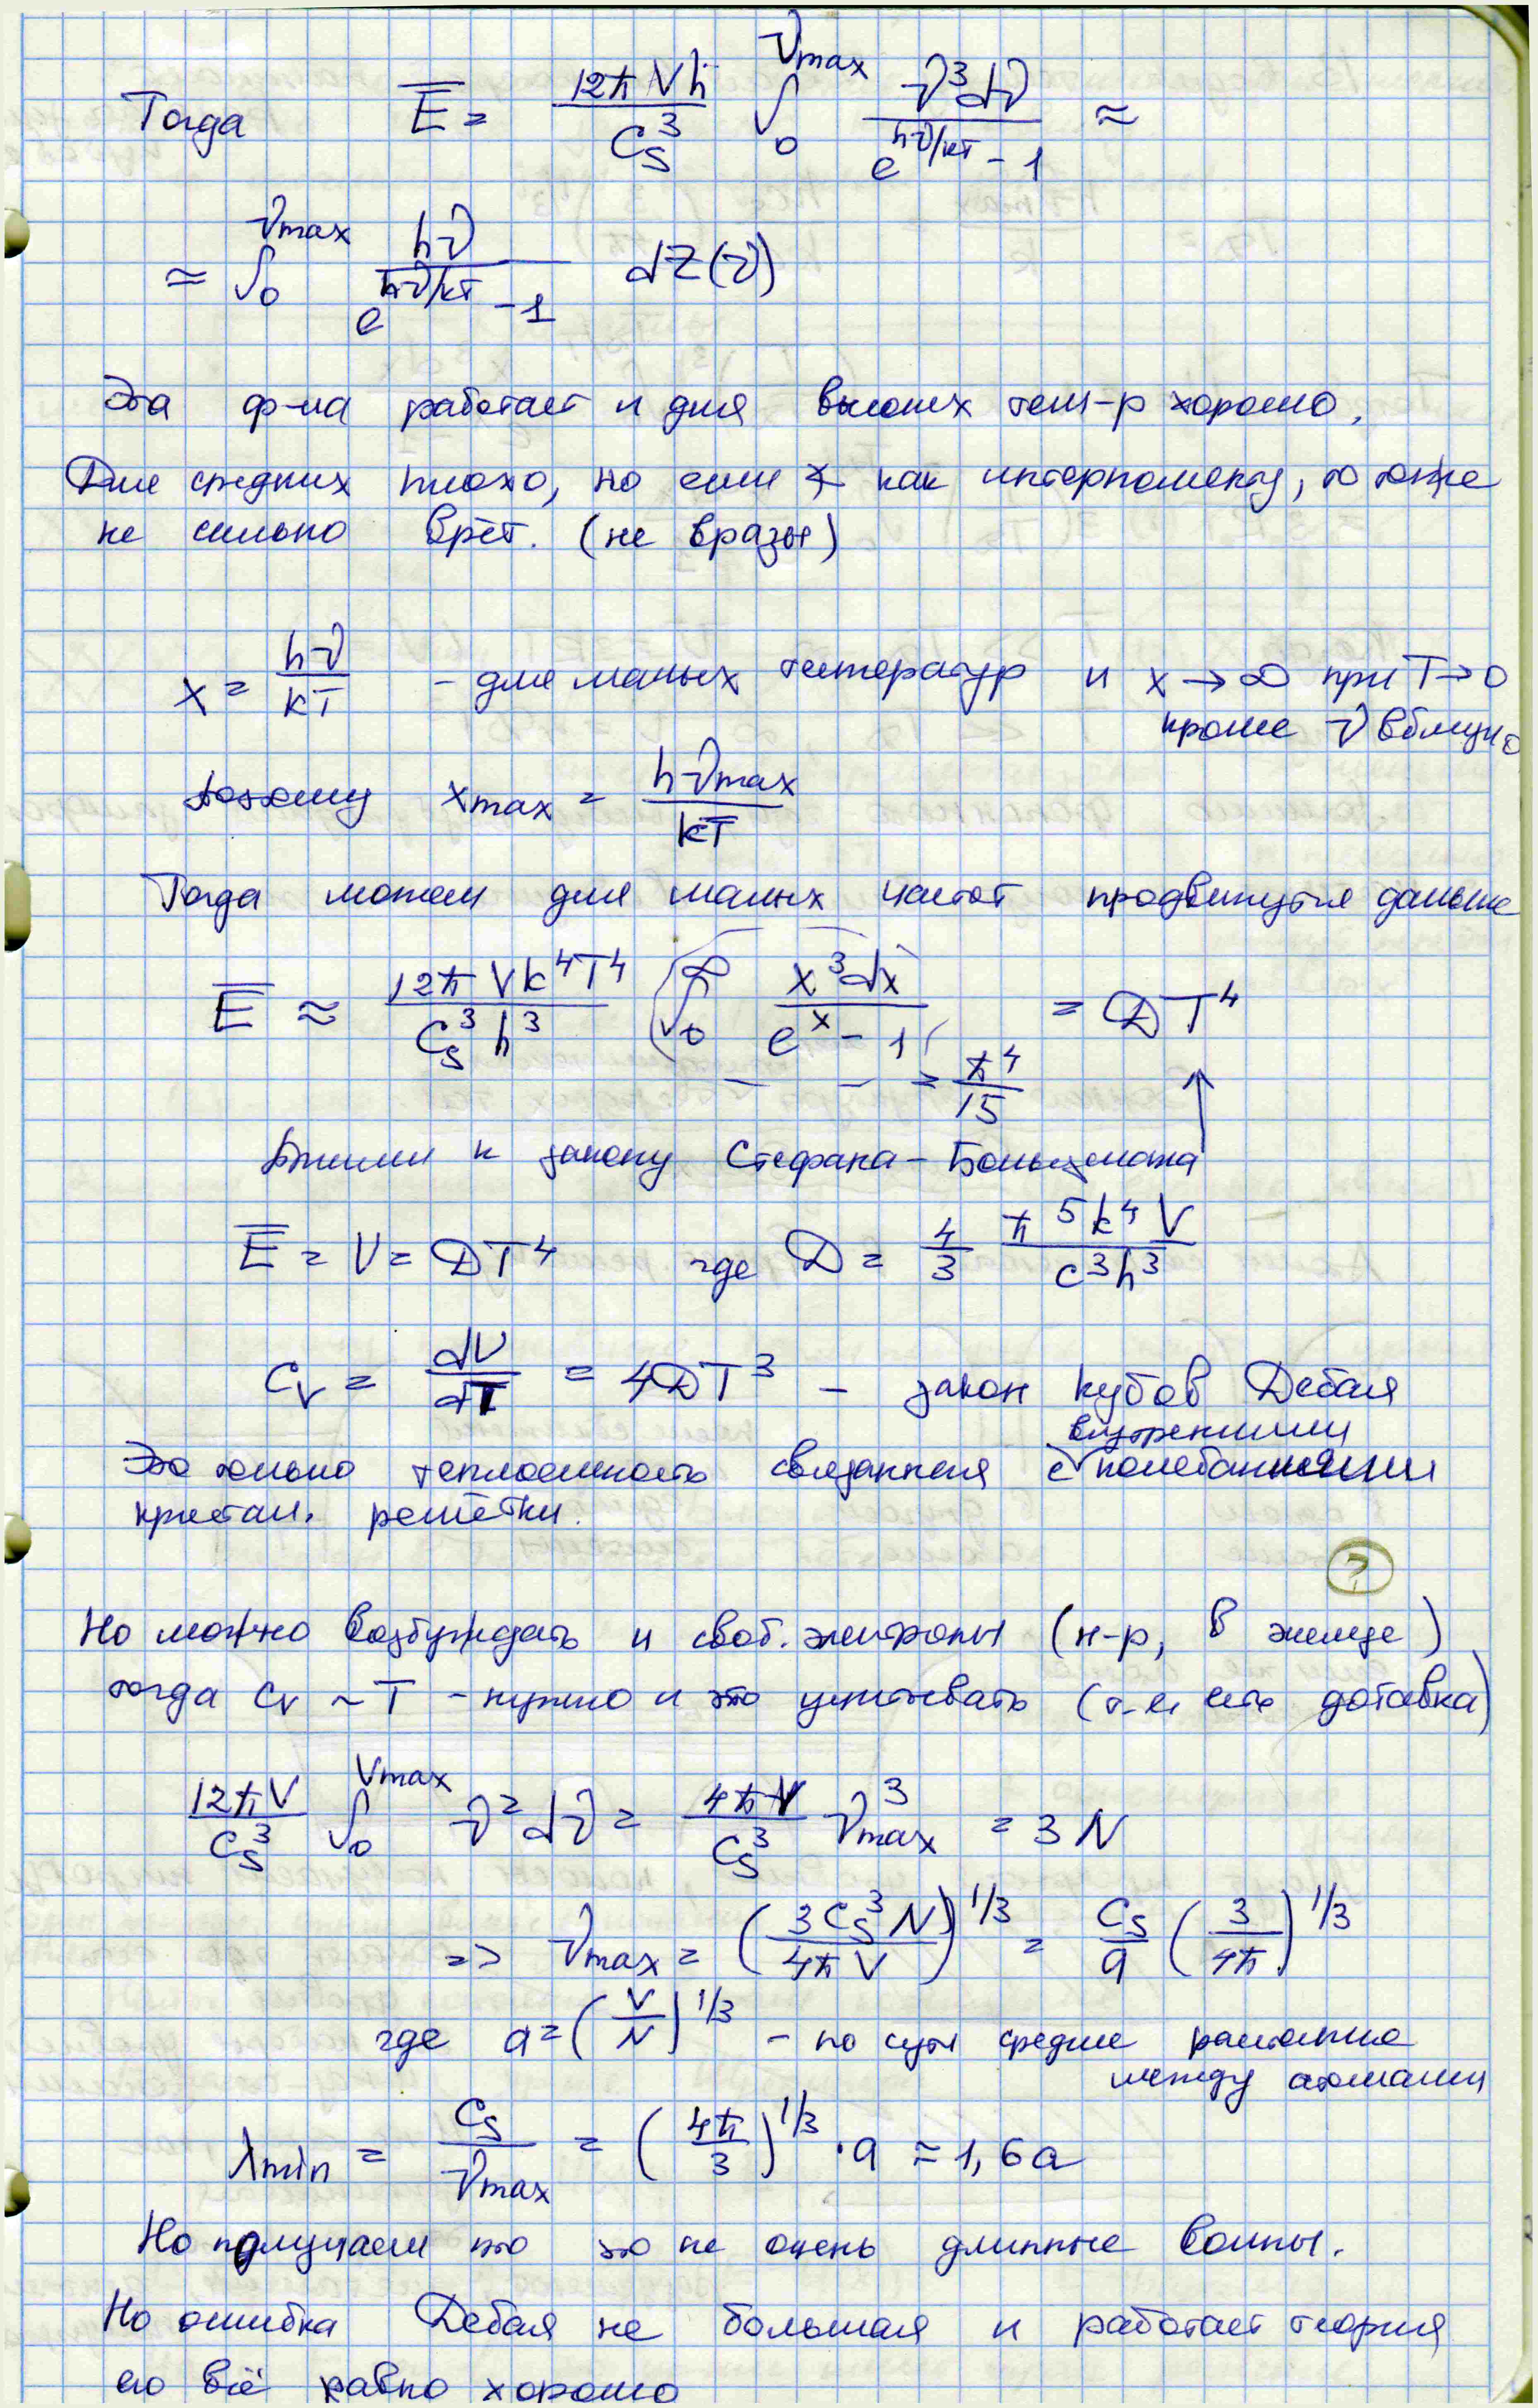
\includegraphics[max size={\textwidth}{0.995\textheight}]{jpg/34.jpg}%
\newpage%
%
%
\phantomsection\addcontentsline{toc}{subsection}{Зонная структура кристаллических твердых тел. Волны Блоха}%
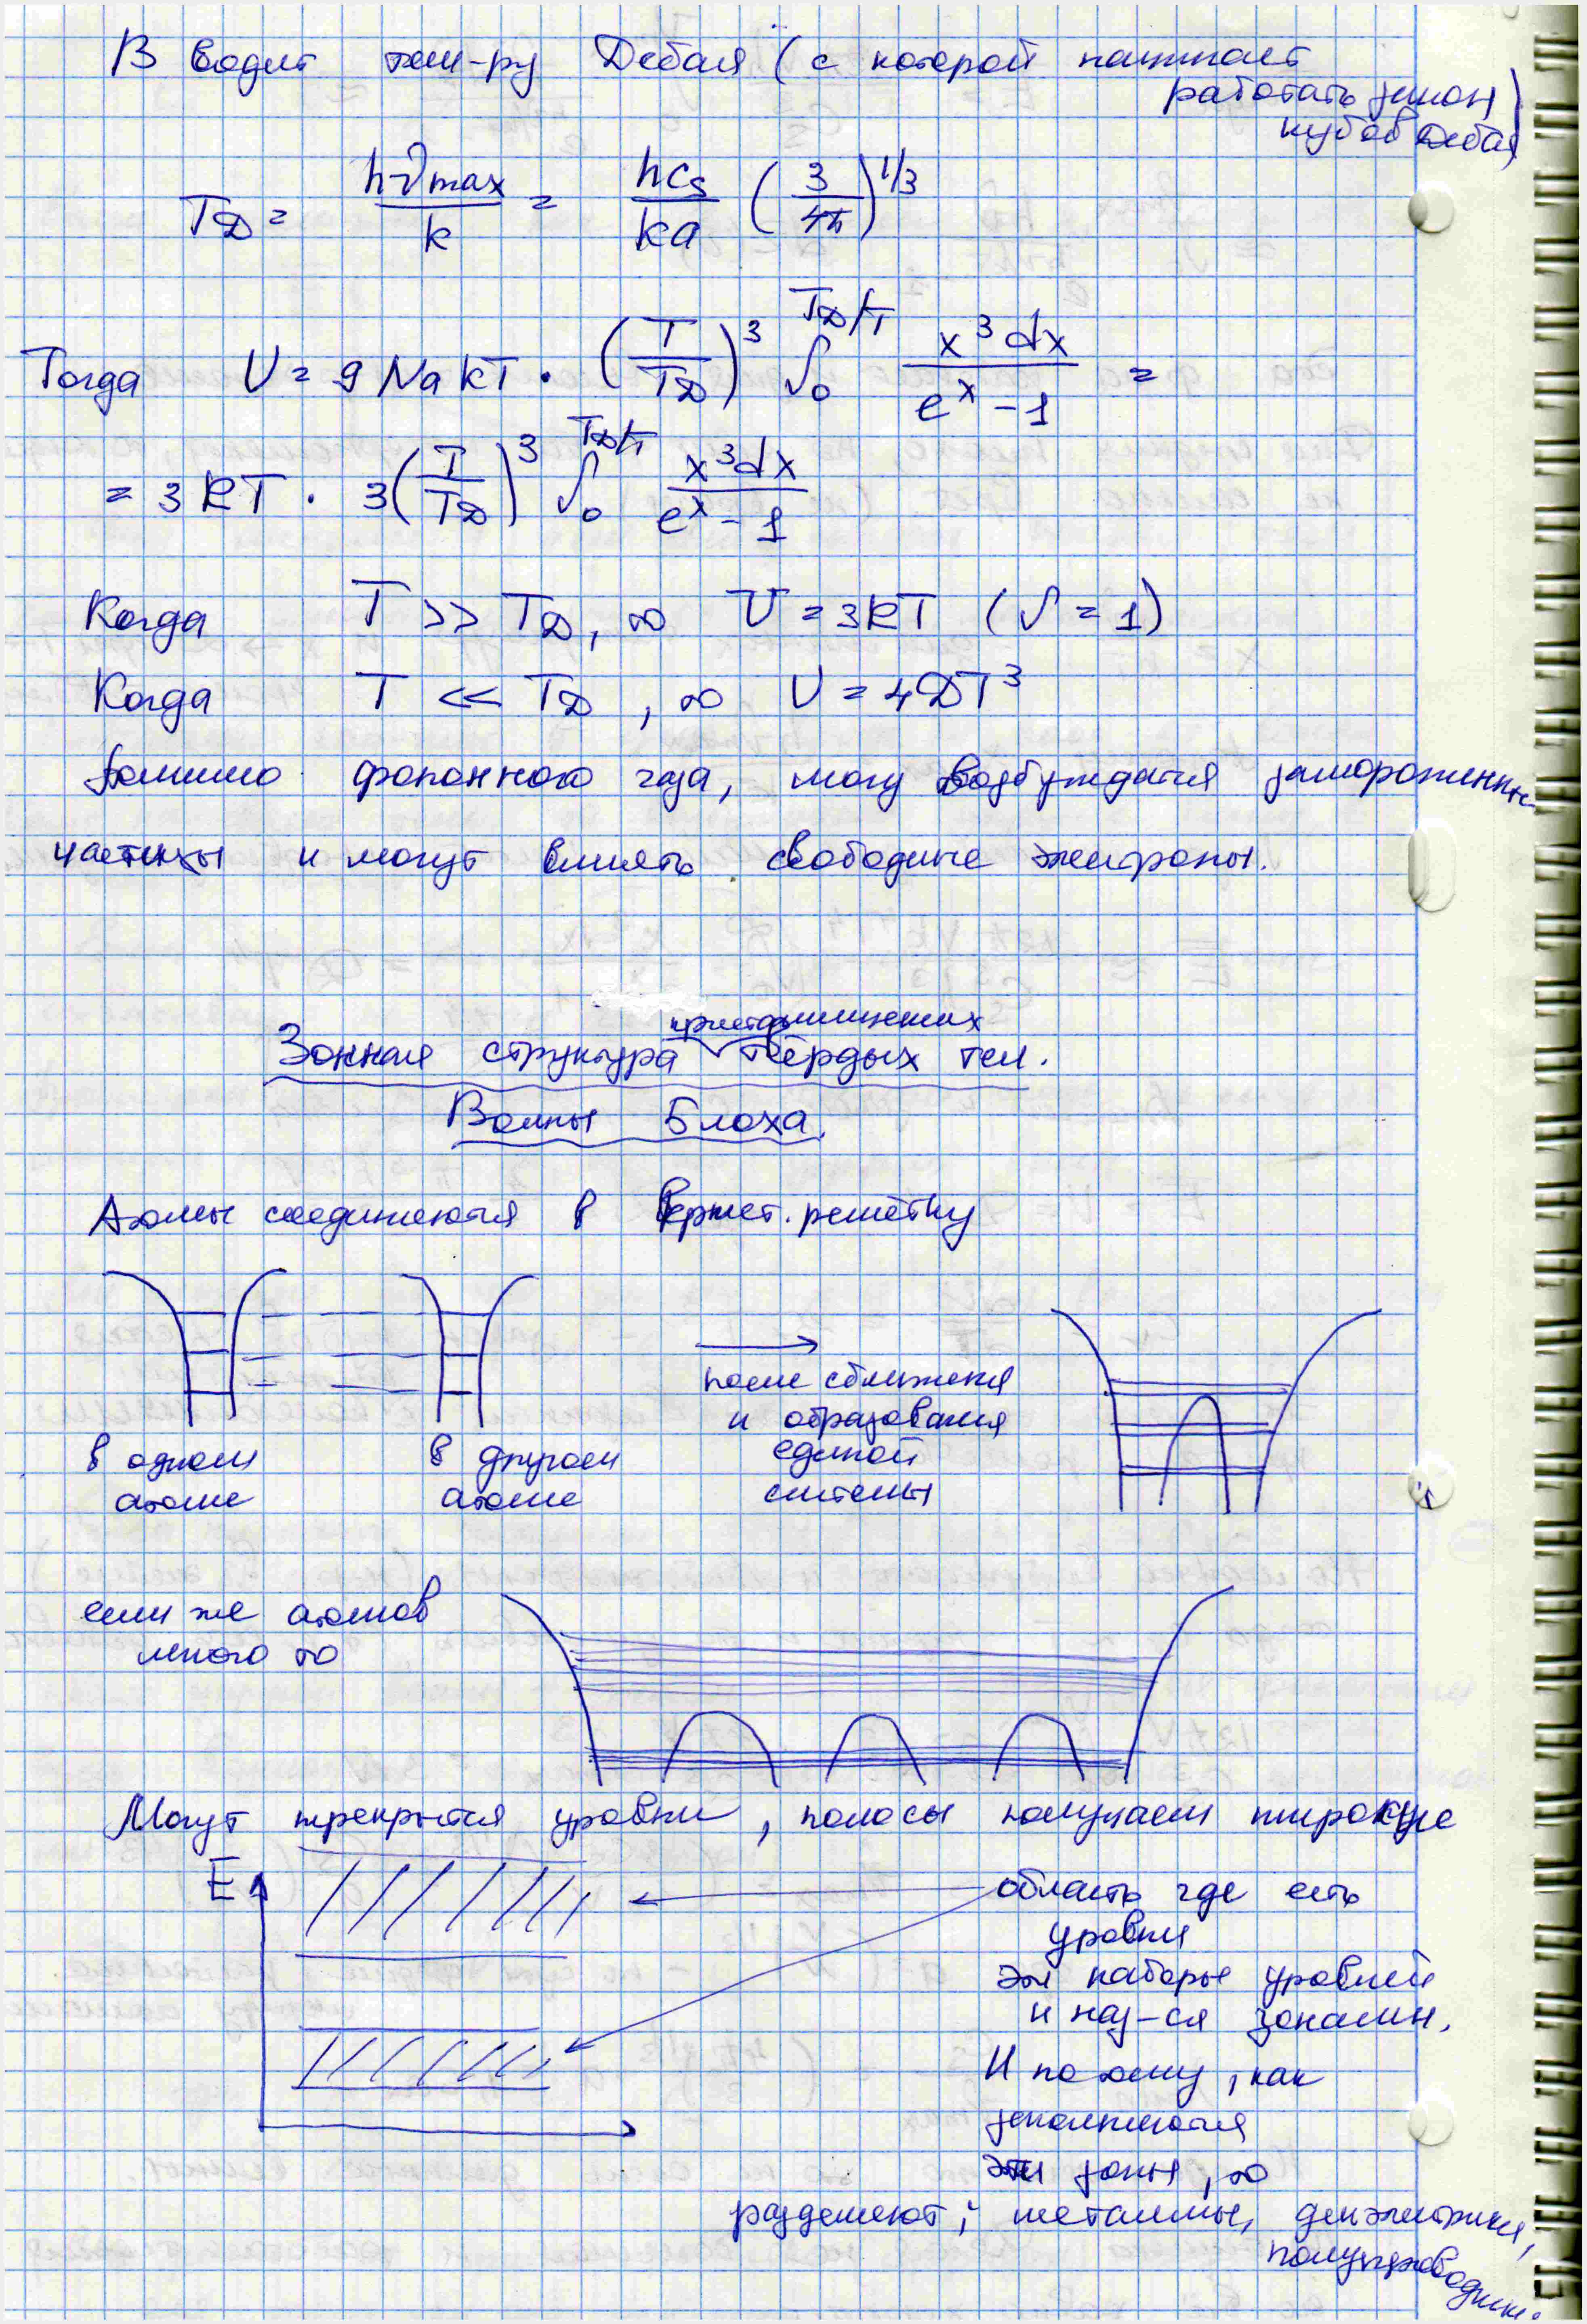
\includegraphics[max size={\textwidth}{0.995\textheight}]{jpg/35.jpg}%
\newpage%
%
%
\phantomsection\addcontentsline{toc}{subsubsection}{Волны Блоха (электрон в периодическом потенциале)}%
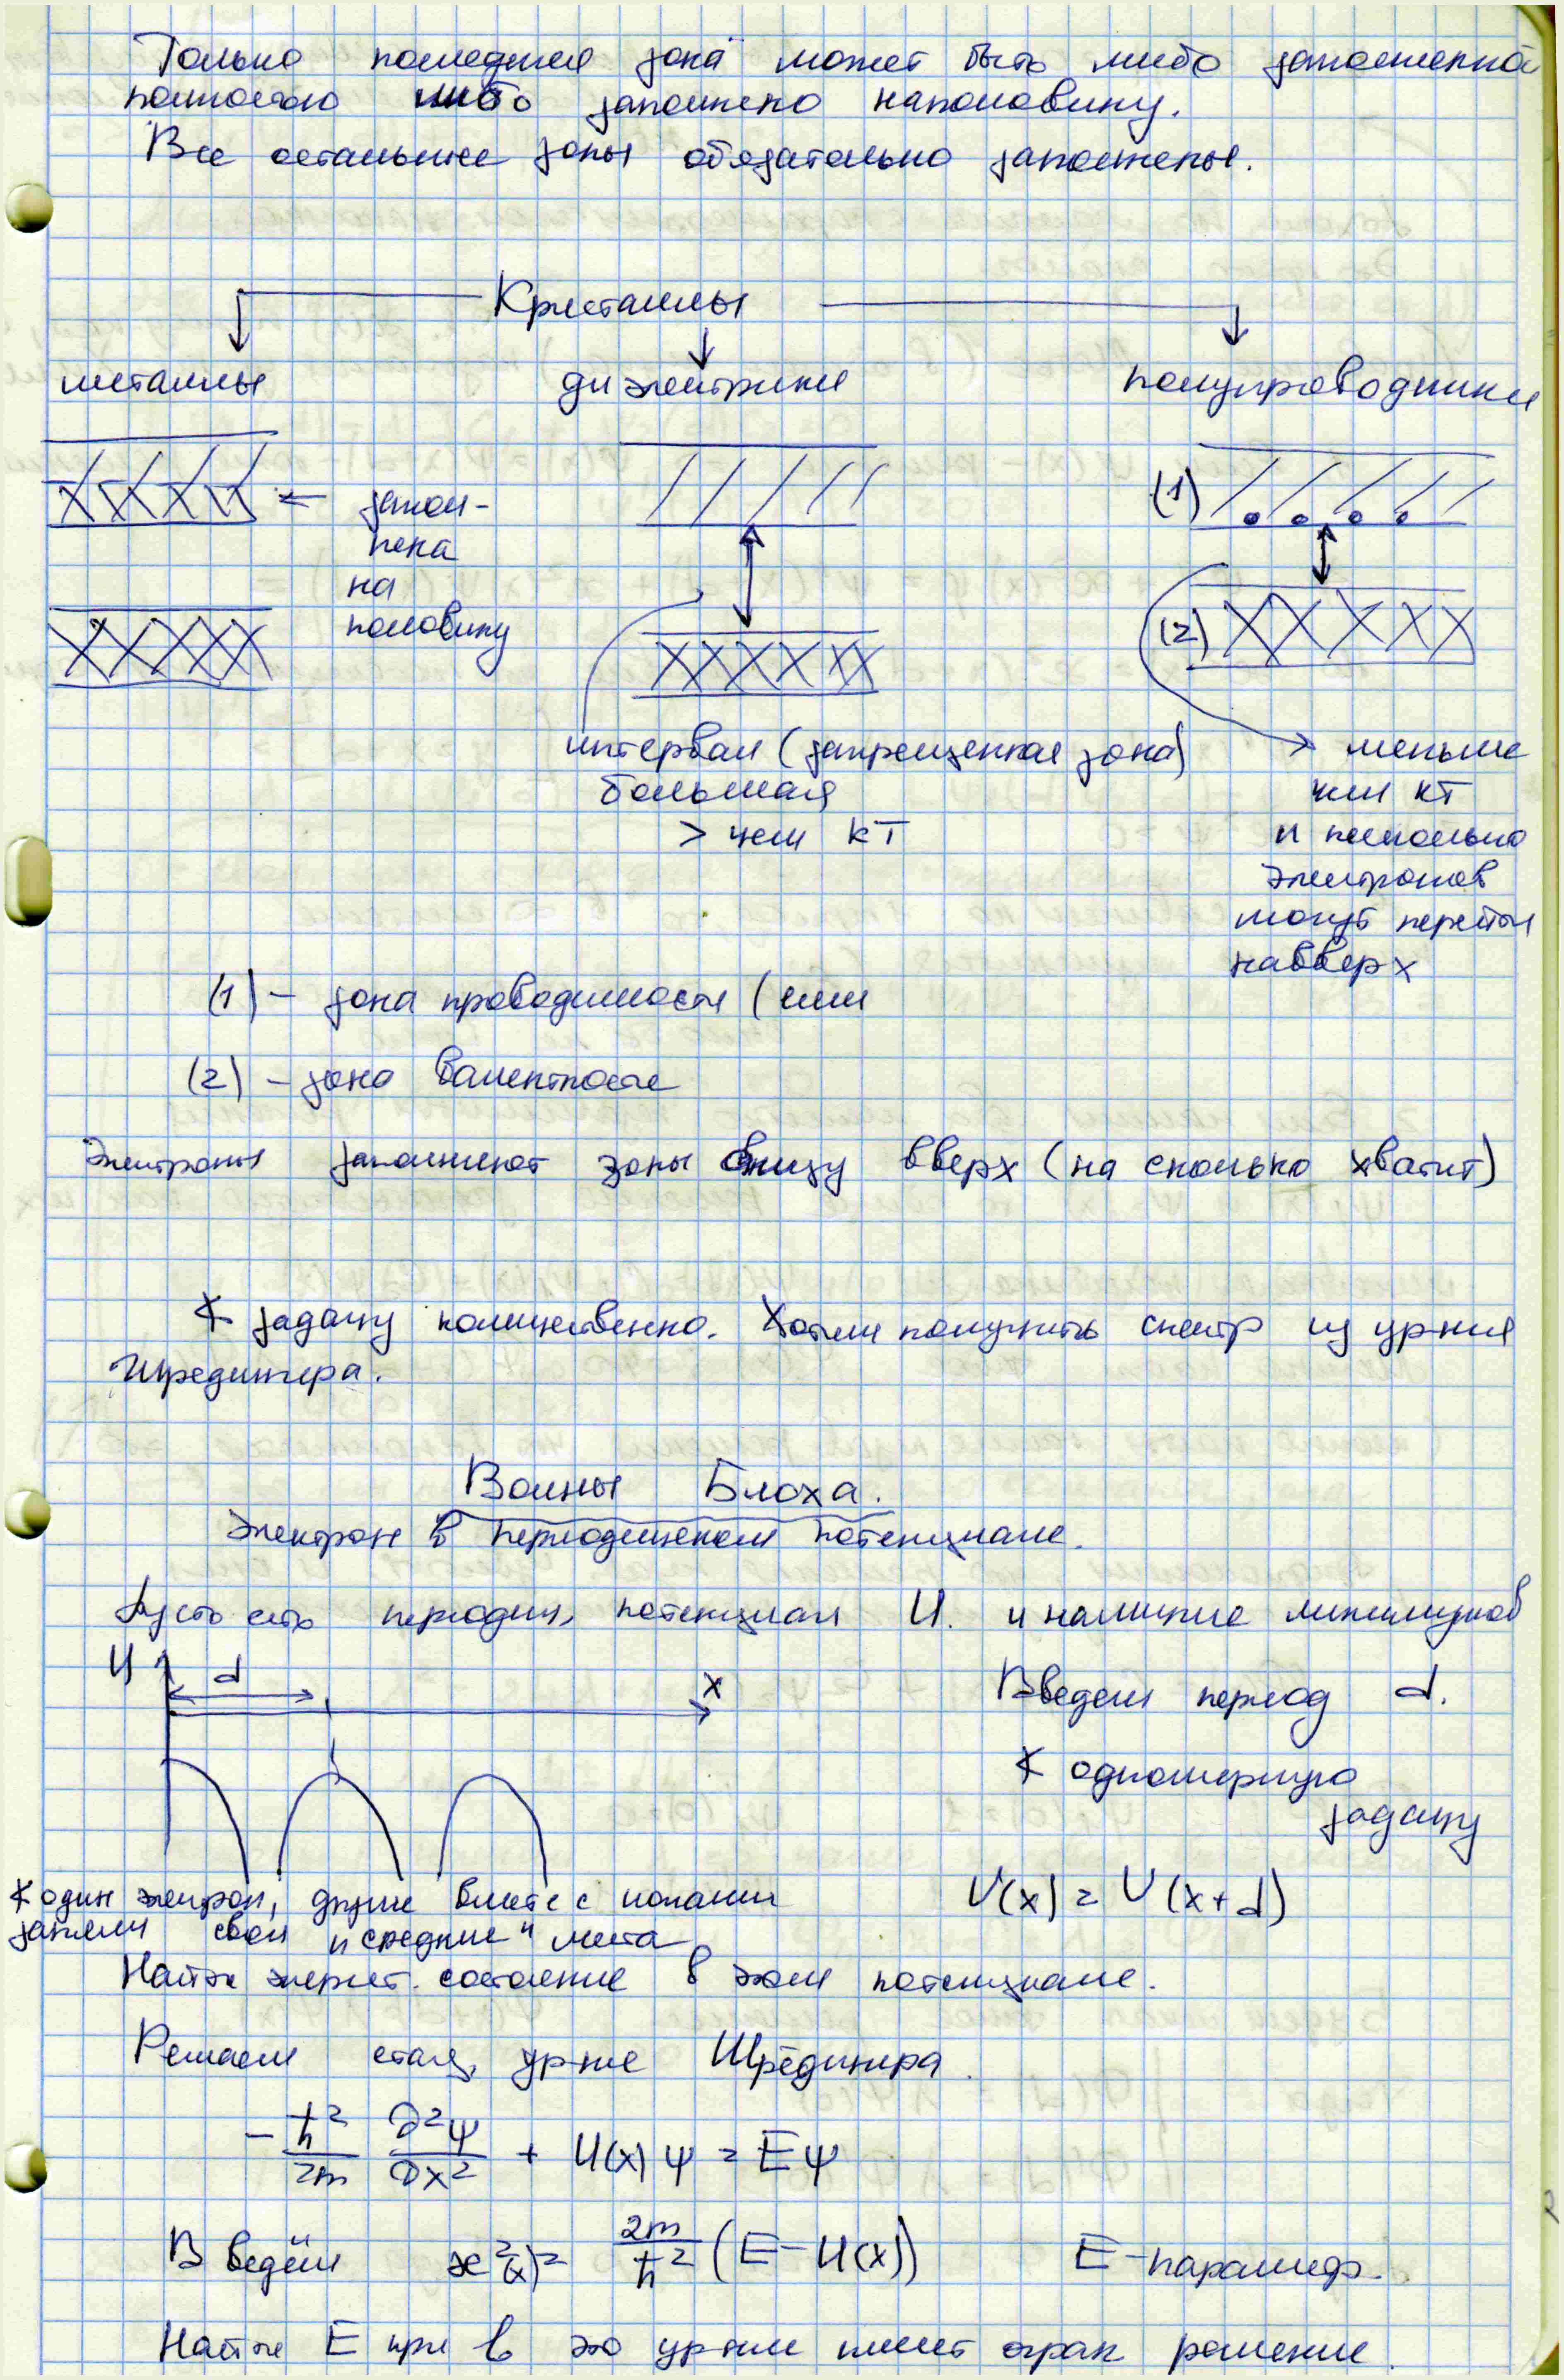
\includegraphics[max size={\textwidth}{0.995\textheight}]{jpg/36.jpg}%
\newpage%
%
%
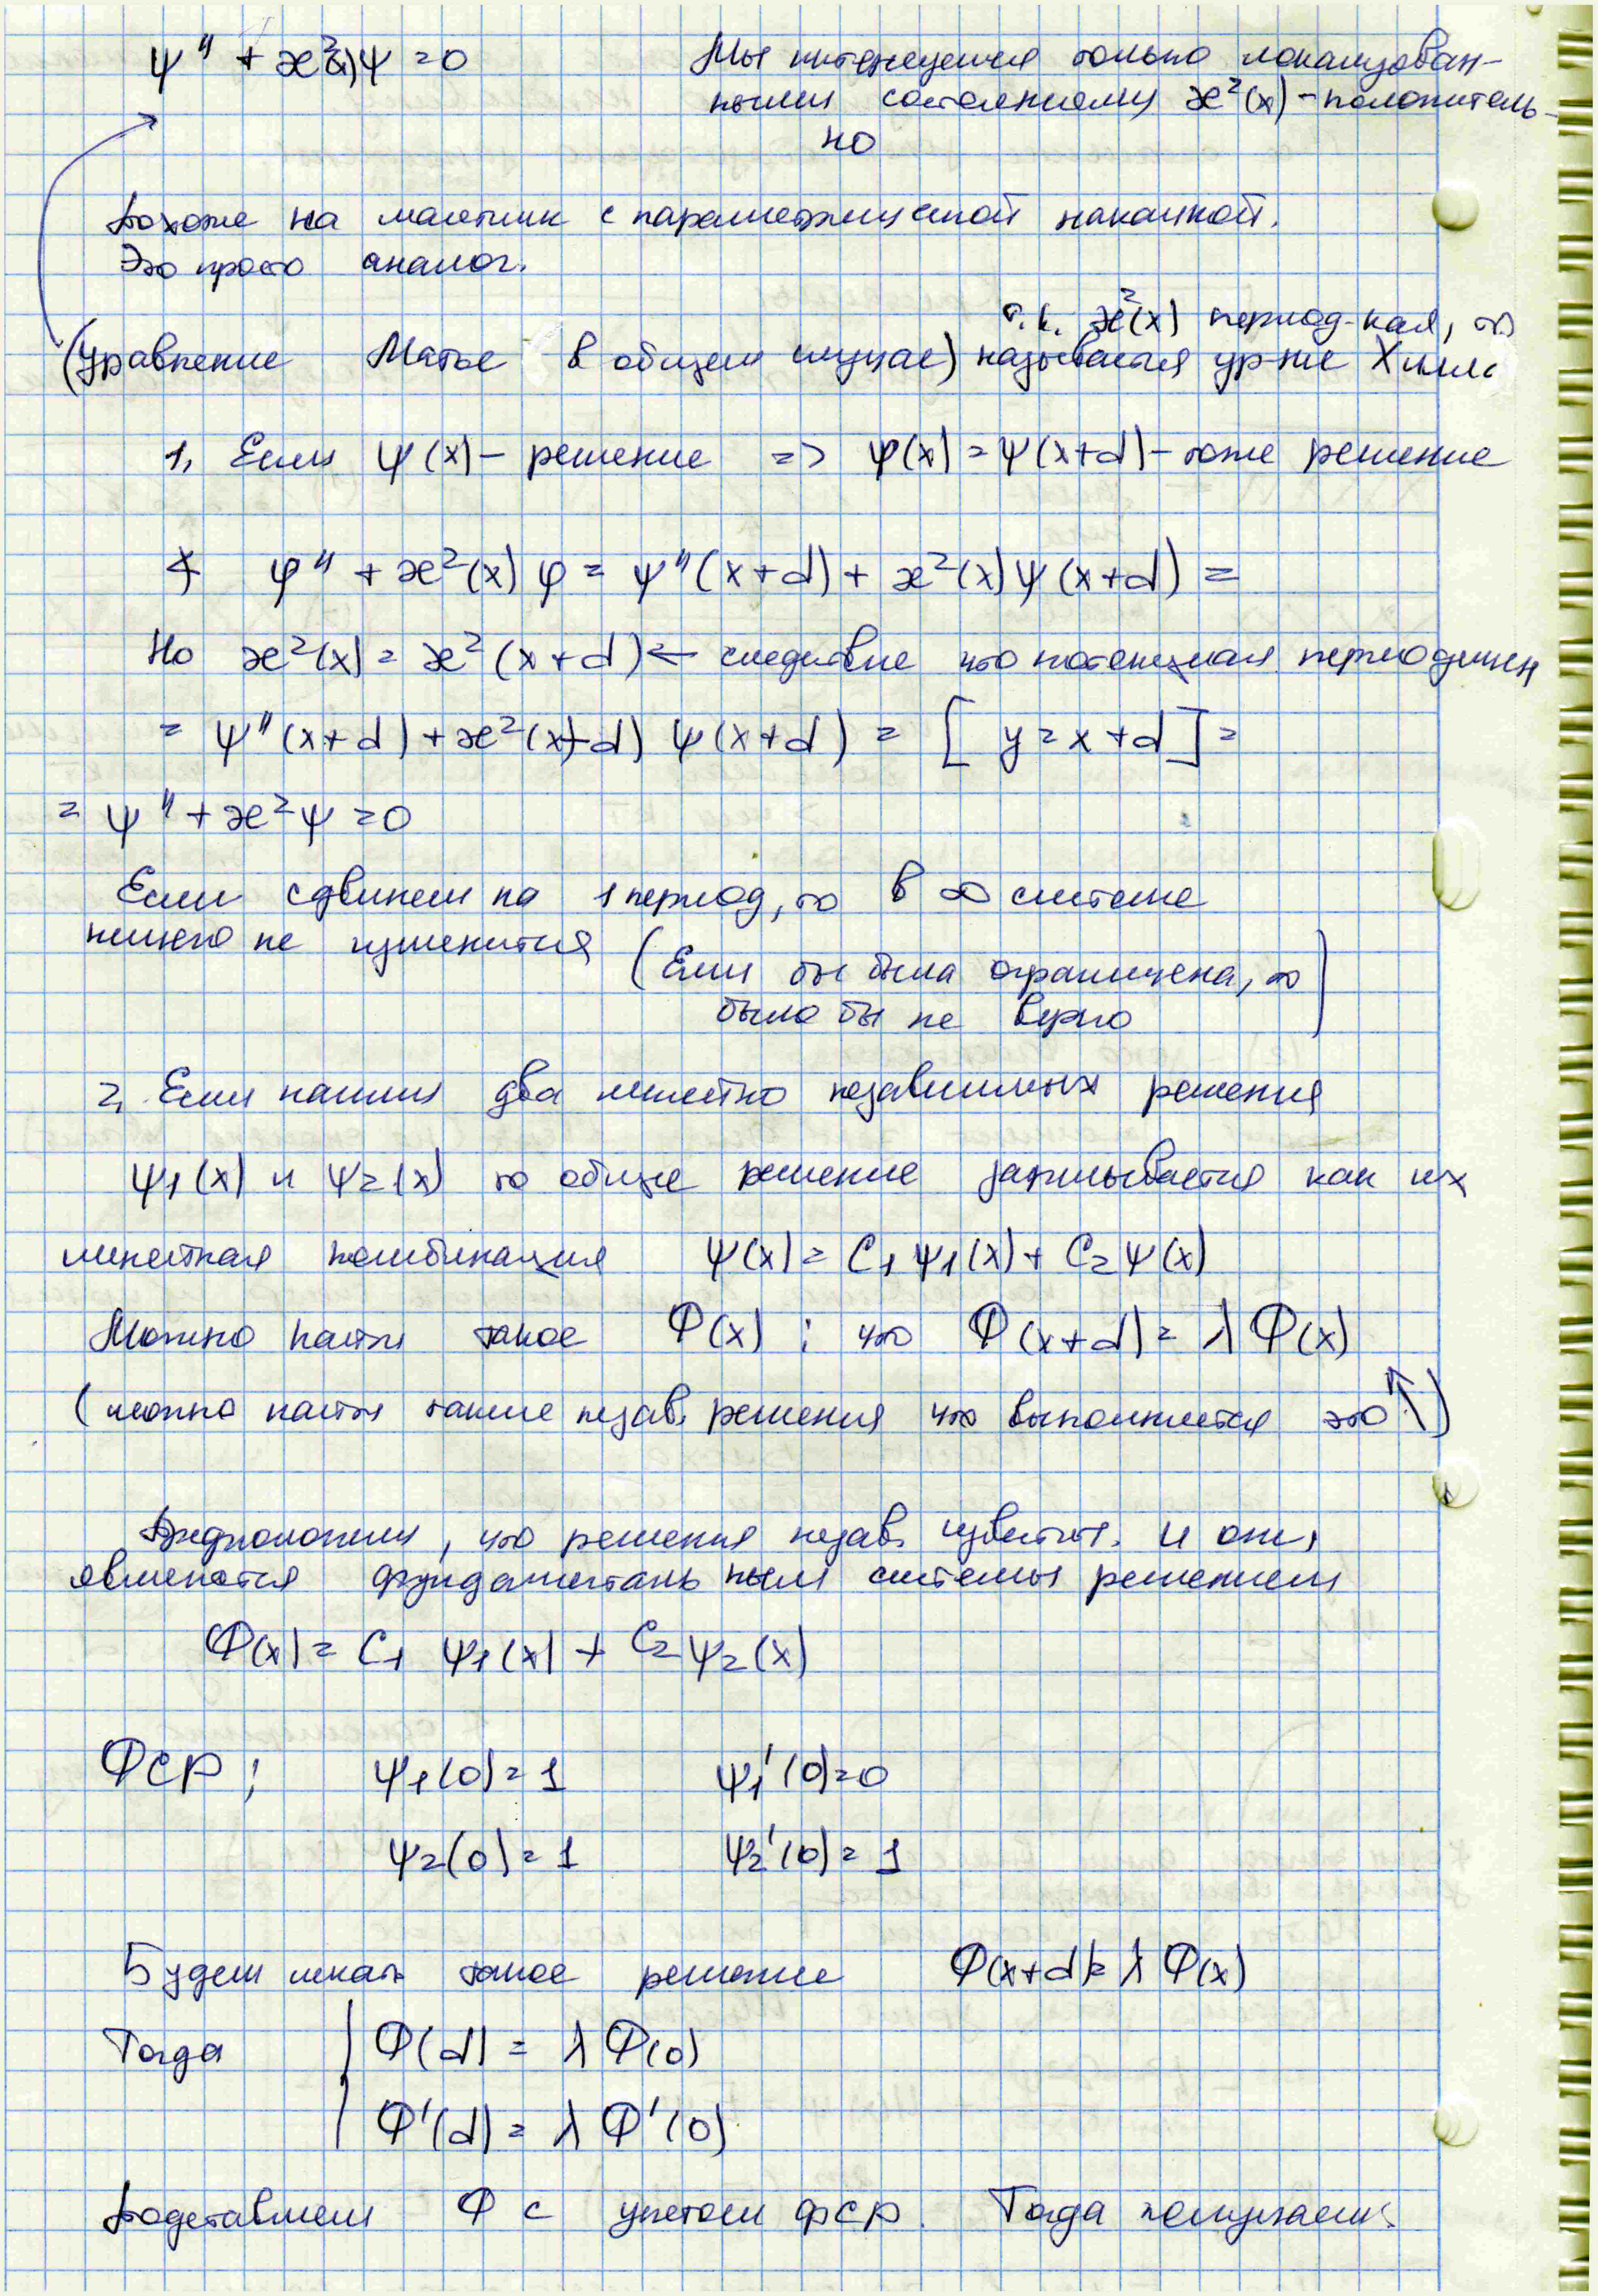
\includegraphics[max size={\textwidth}{0.995\textheight}]{jpg/37.jpg}%
\newpage%
%
%
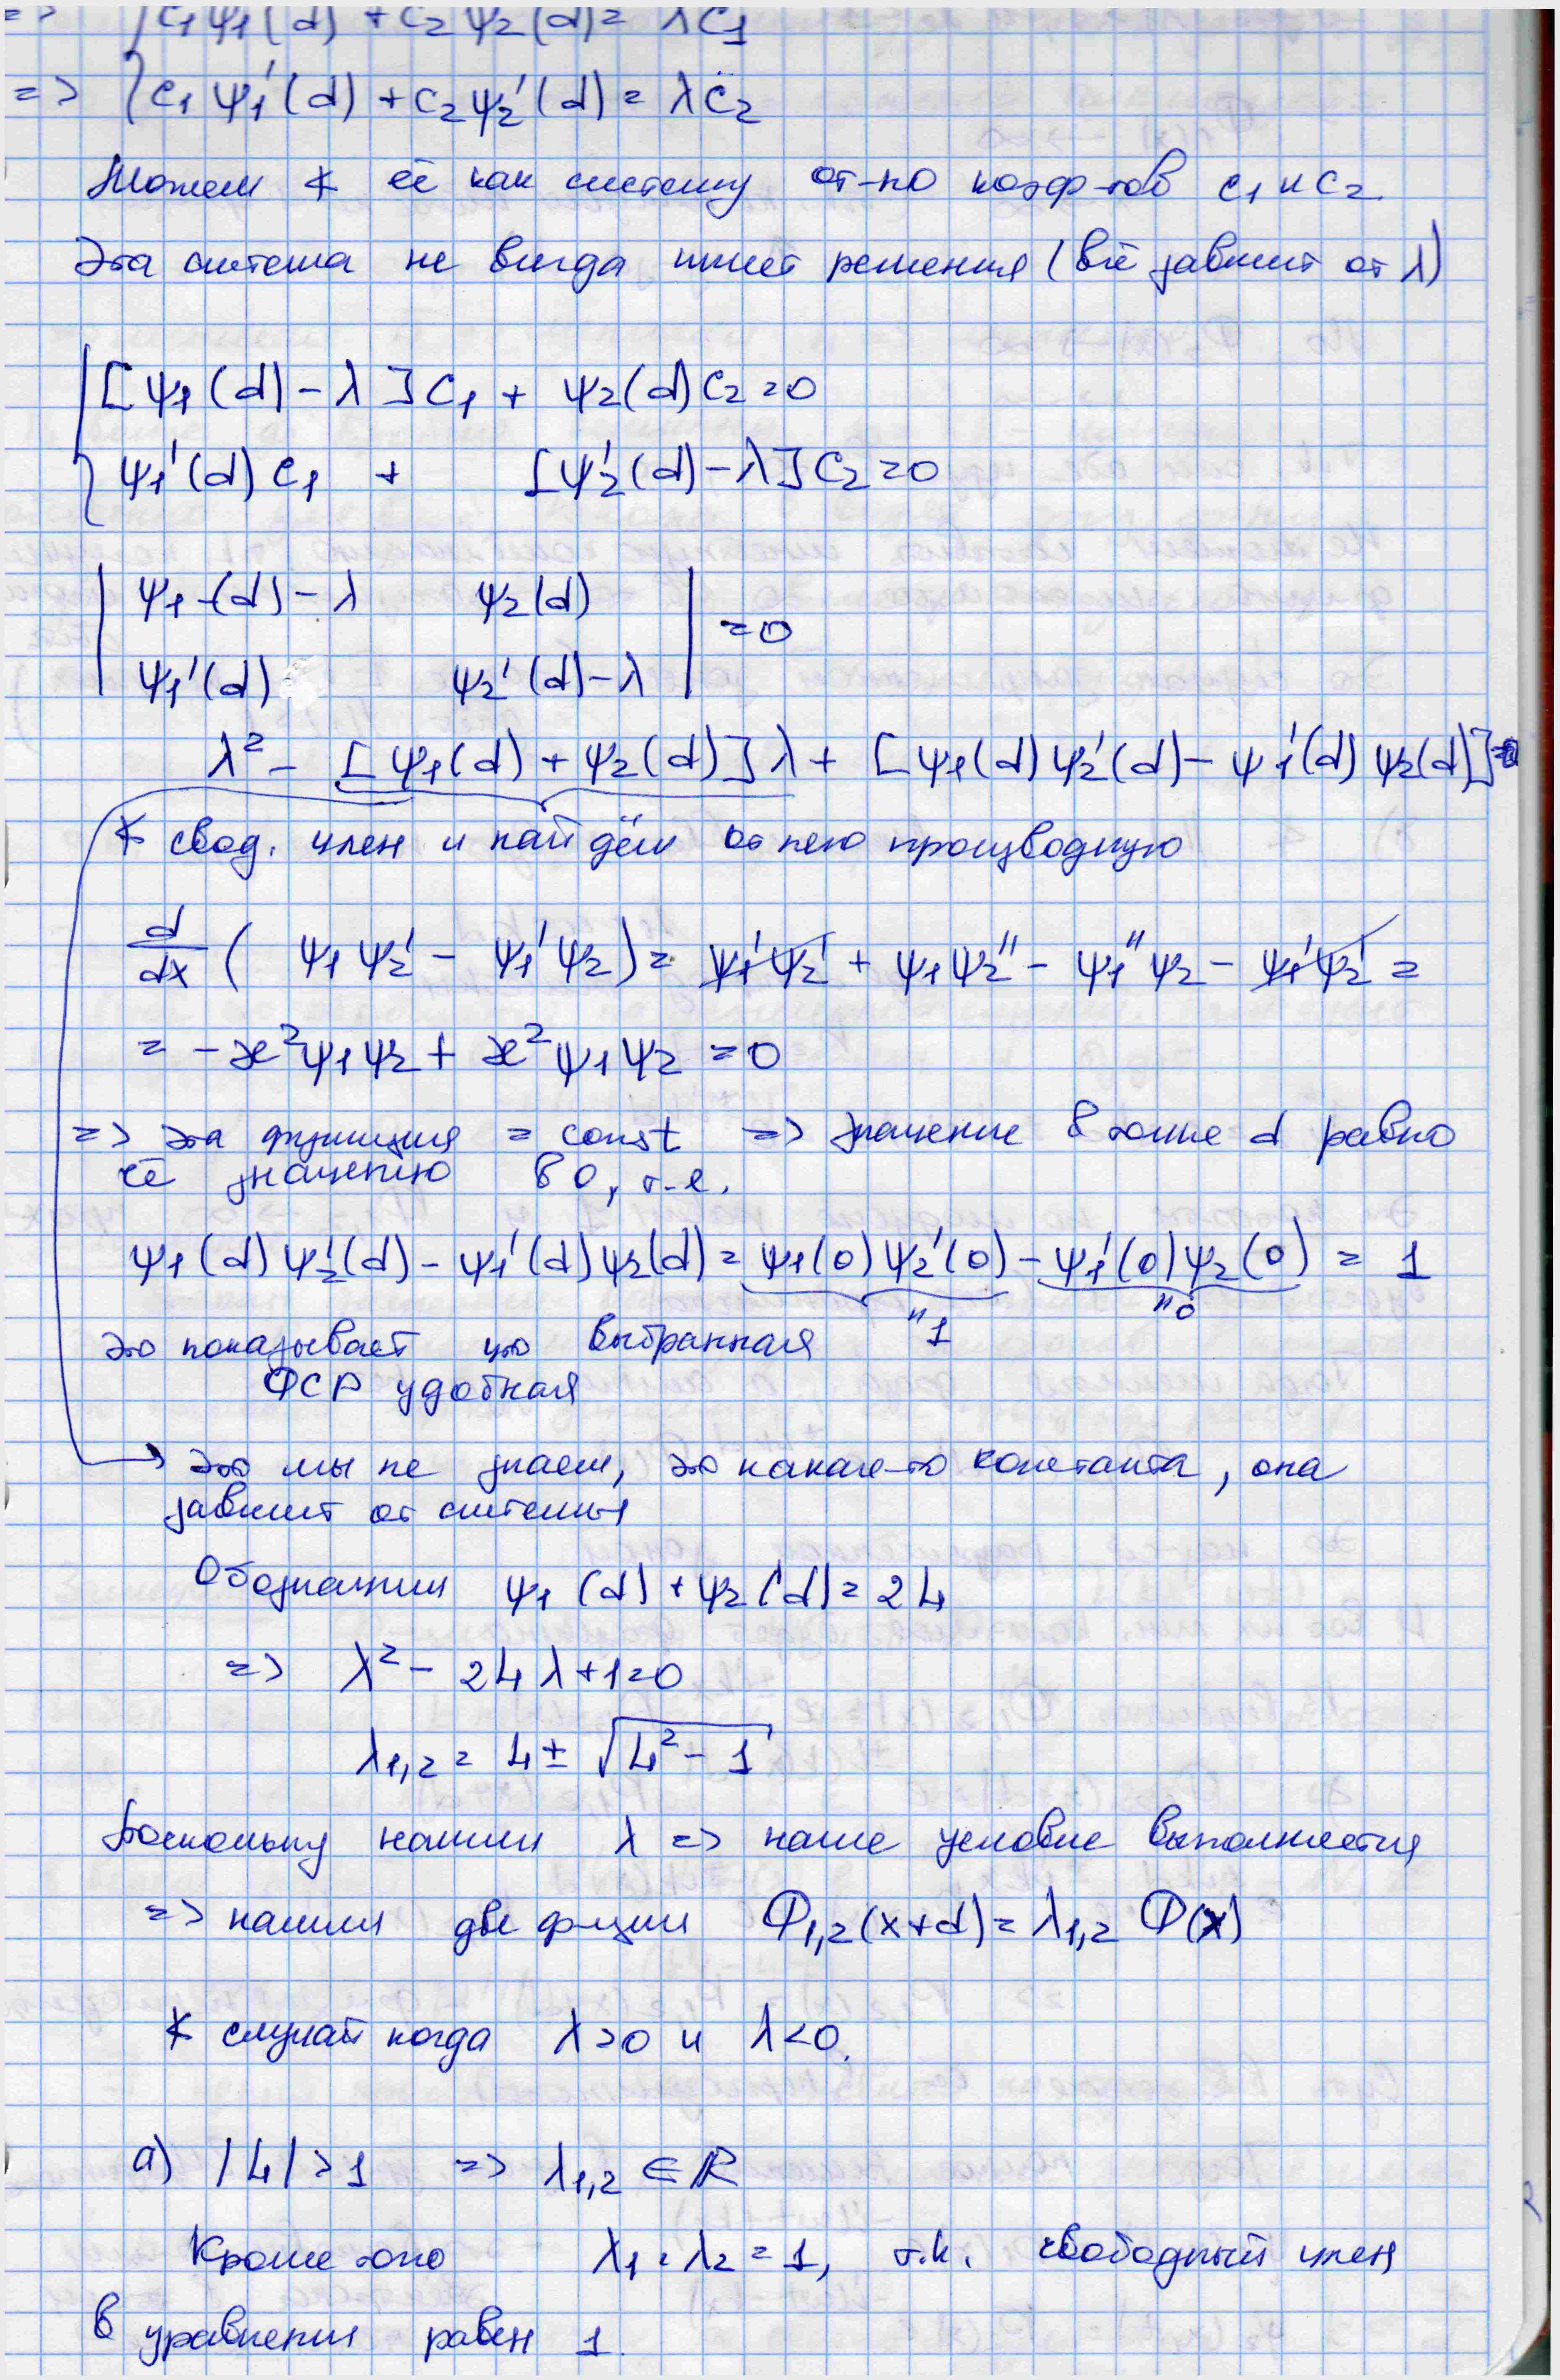
\includegraphics[max size={\textwidth}{0.995\textheight}]{jpg/38.jpg}%
\newpage%
%
%
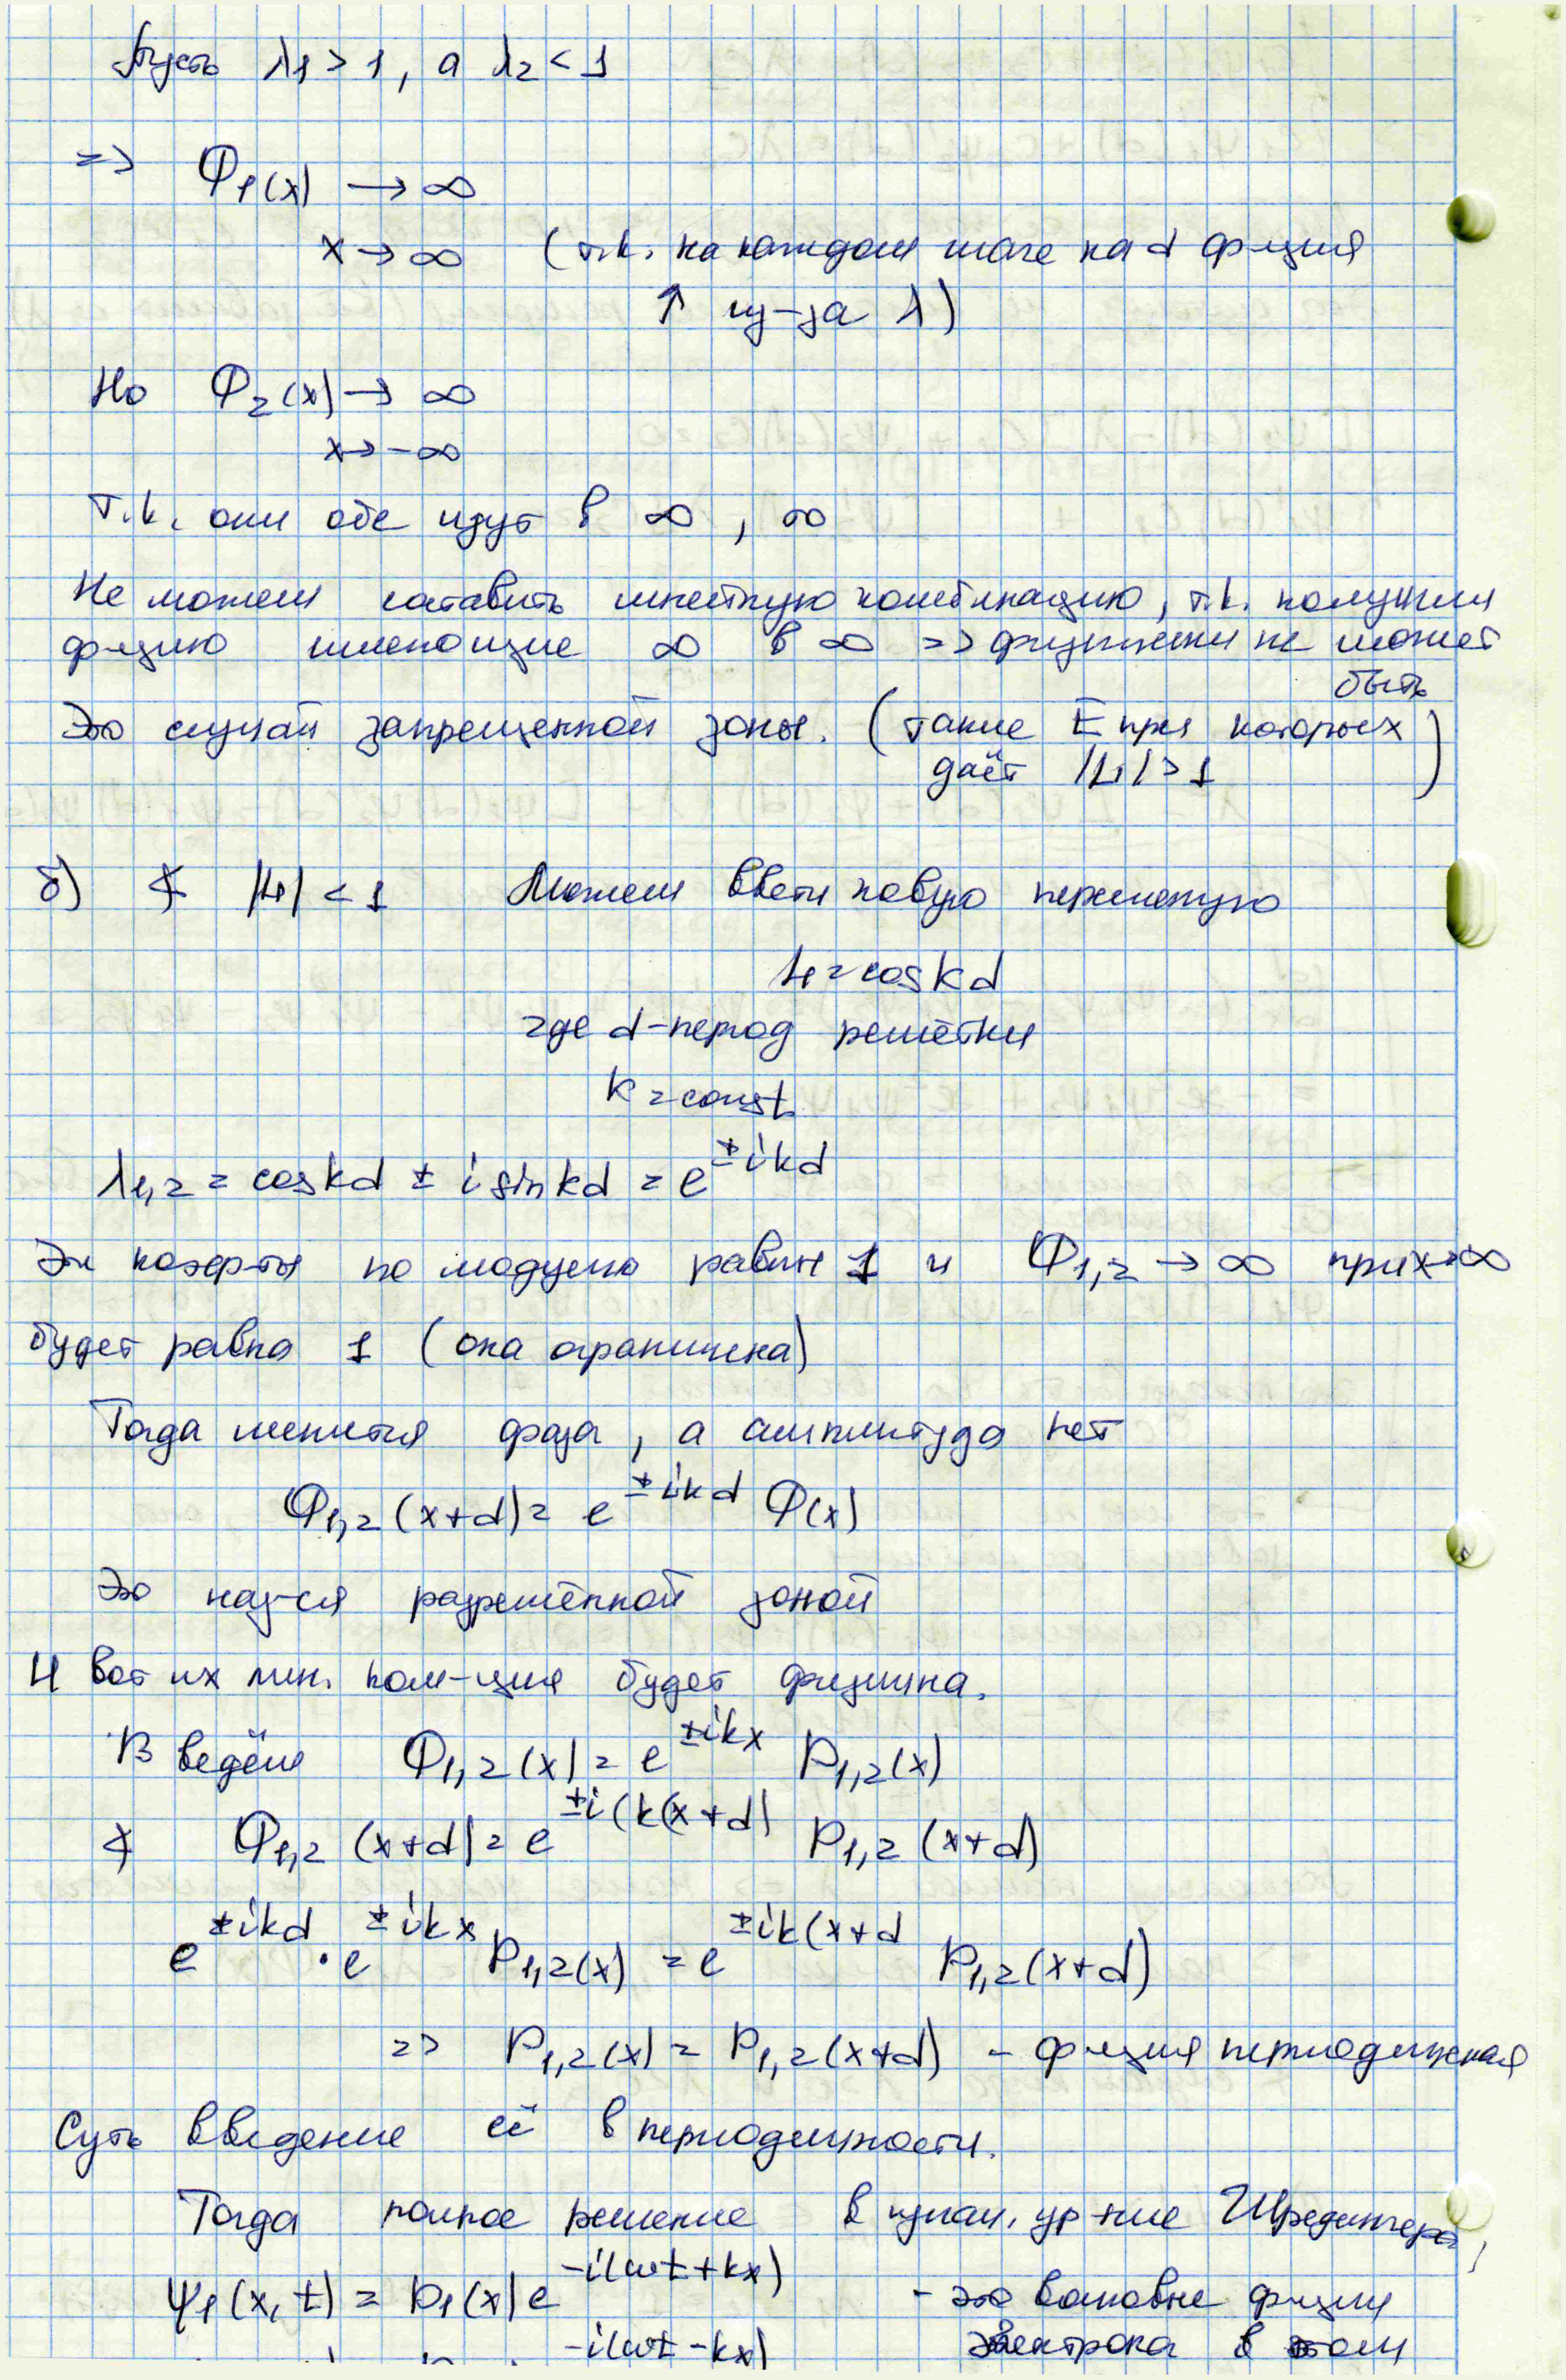
\includegraphics[max size={\textwidth}{0.995\textheight}]{jpg/39.jpg}%
\newpage%
%
%
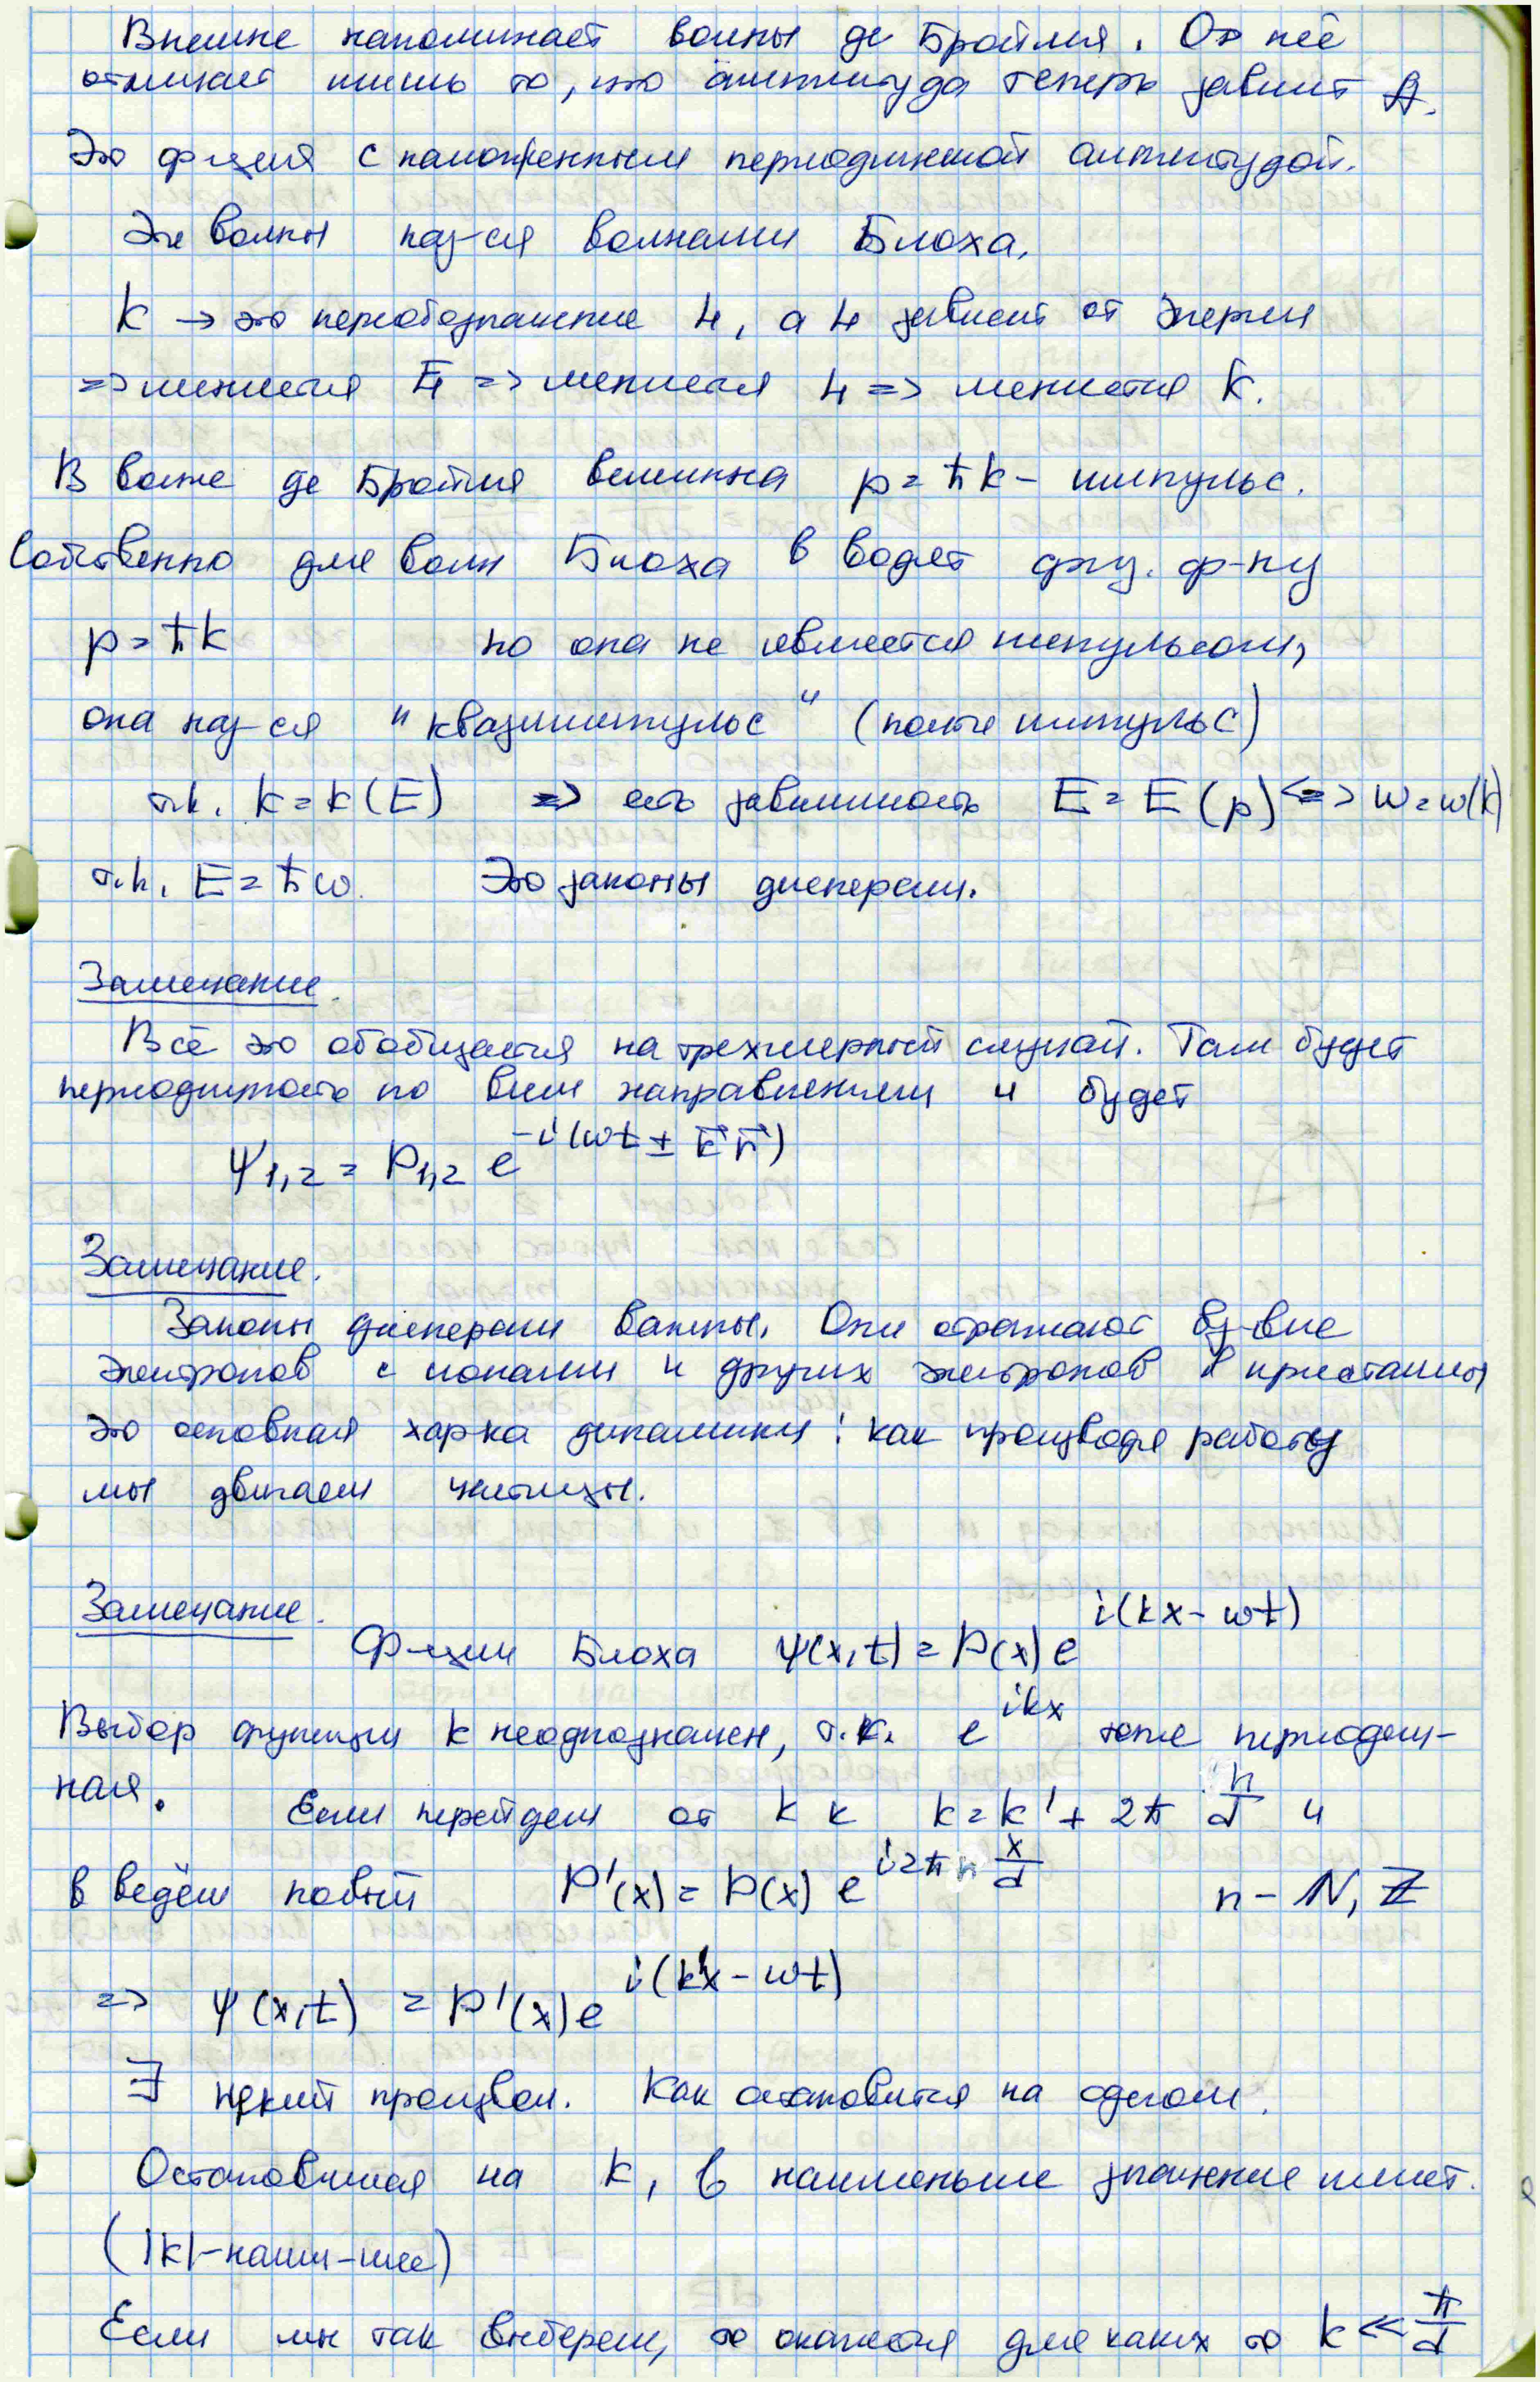
\includegraphics[max size={\textwidth}{0.995\textheight}]{jpg/40.jpg}%
\newpage%
%
%
\phantomsection\addcontentsline{toc}{subsection}{Электропроводность}%
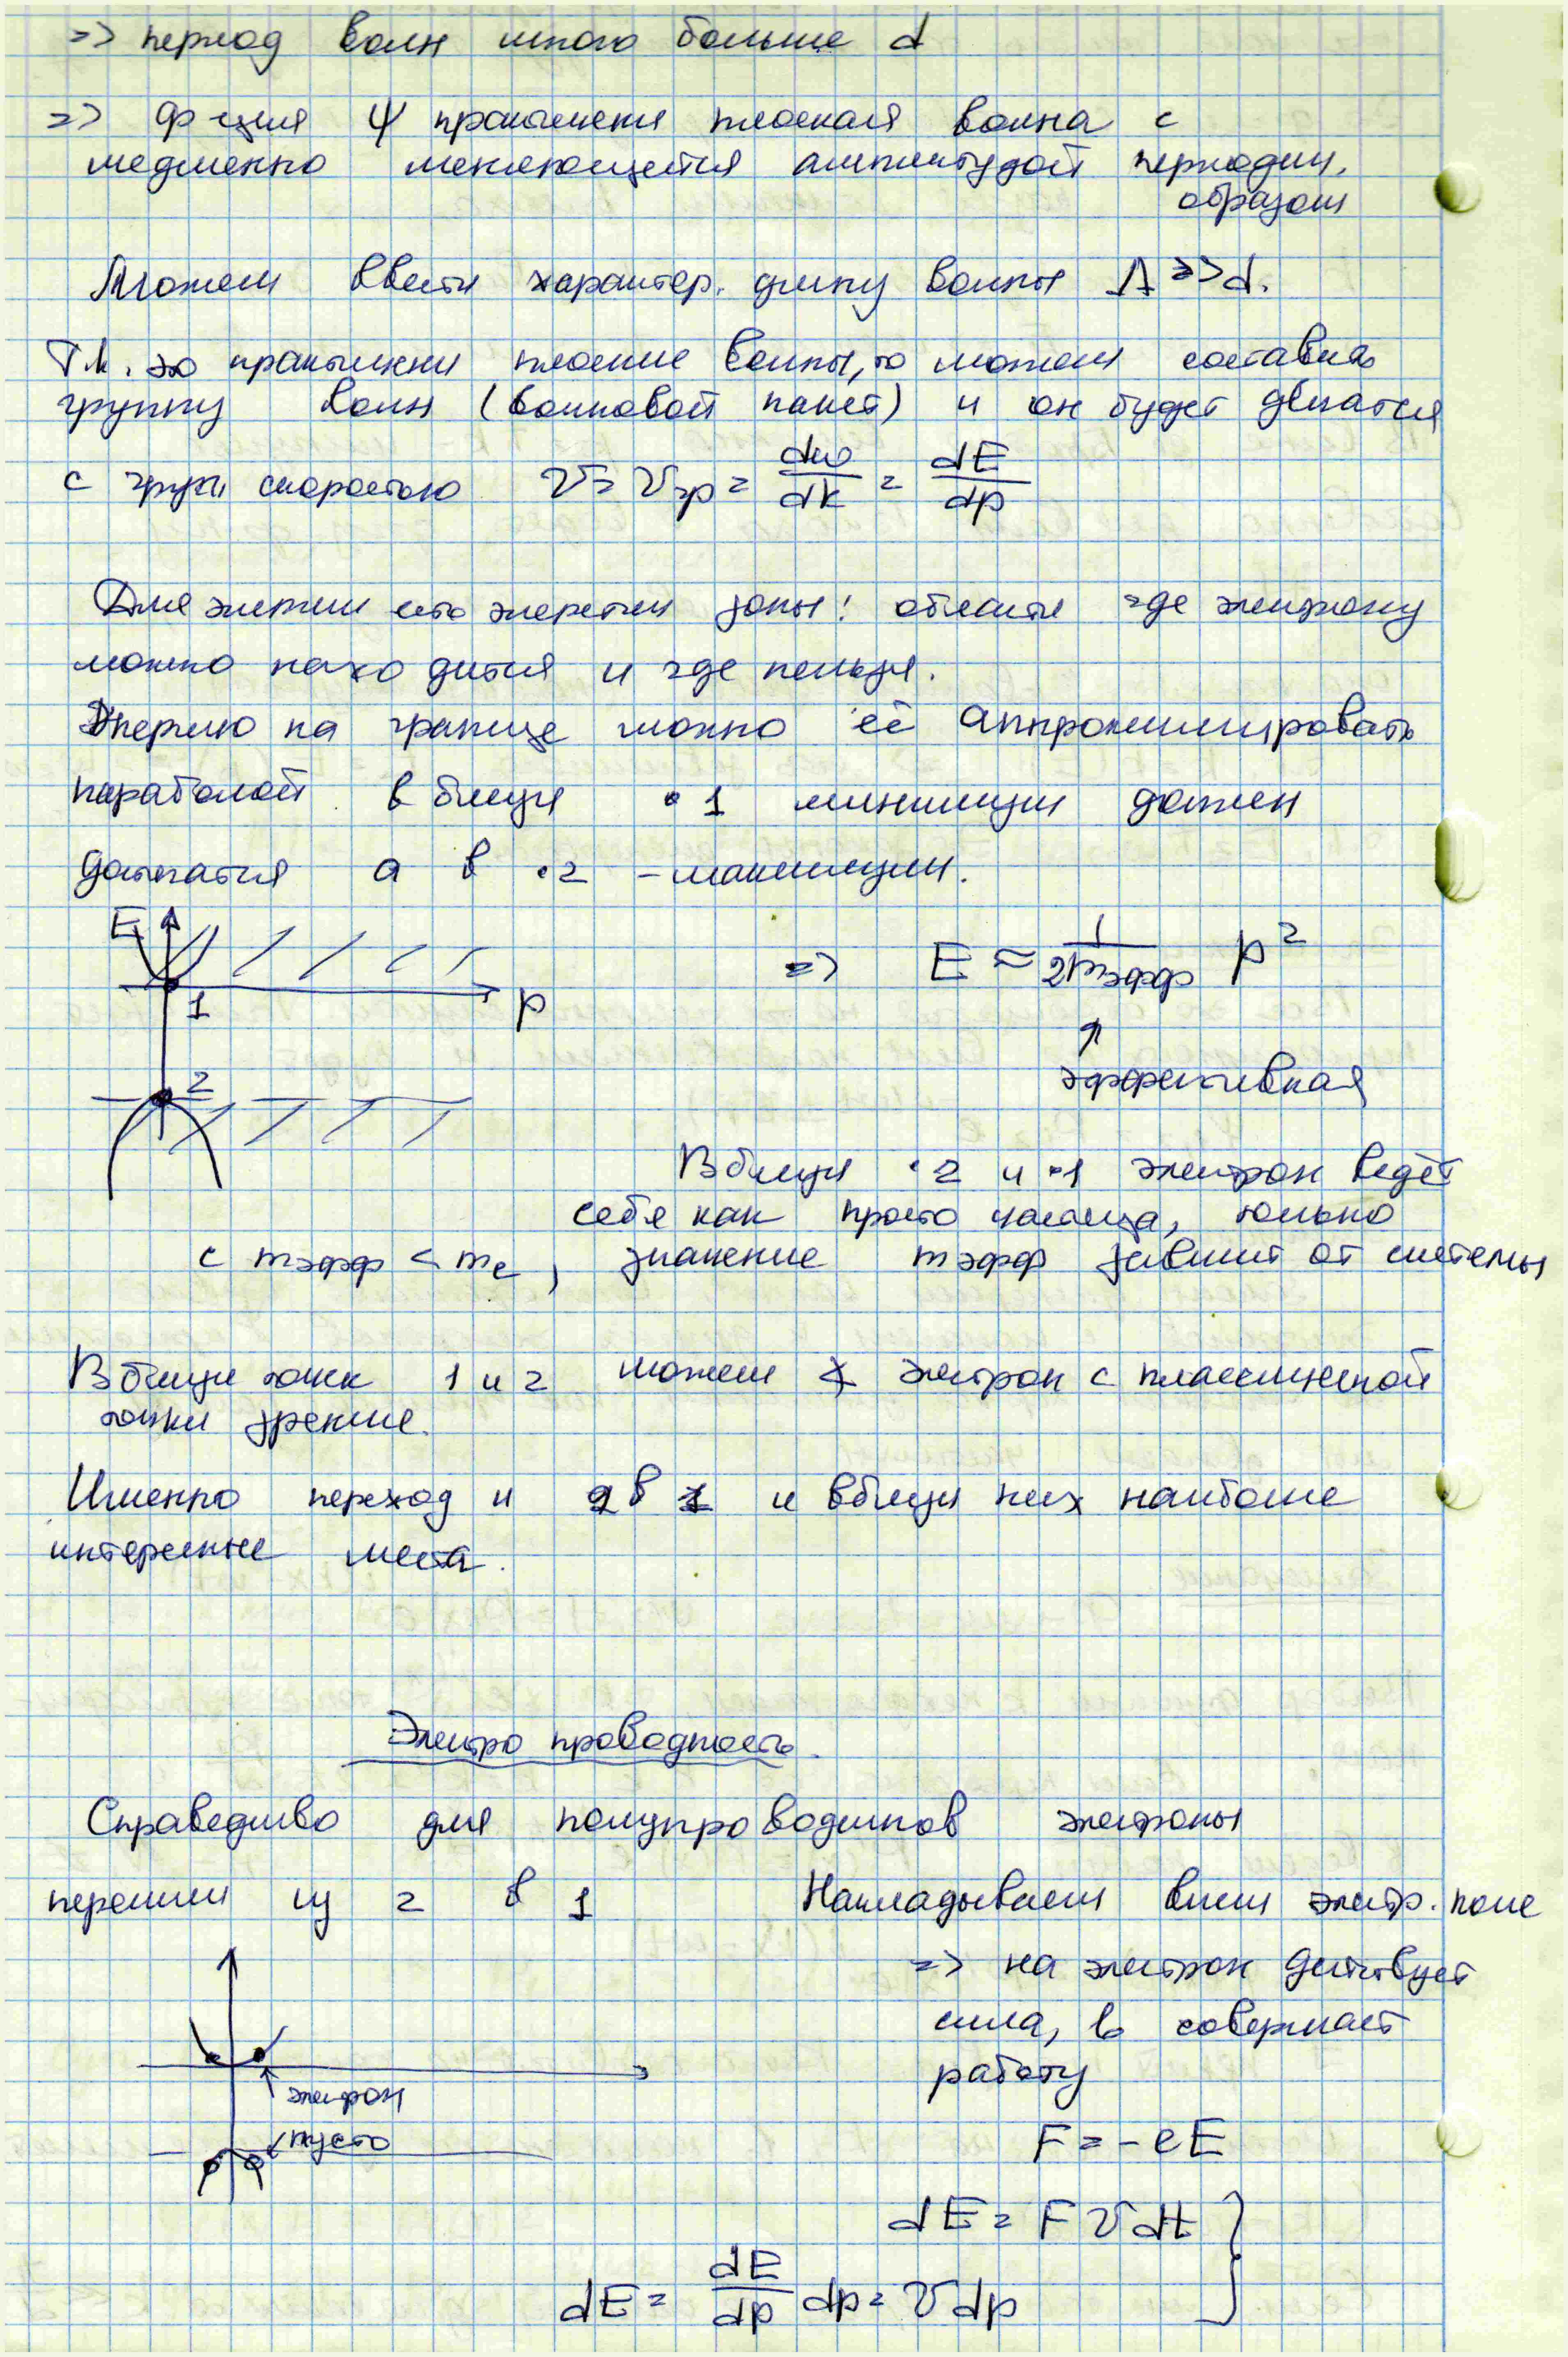
\includegraphics[max size={\textwidth}{0.995\textheight}]{jpg/41.jpg}%
\newpage%
%
%
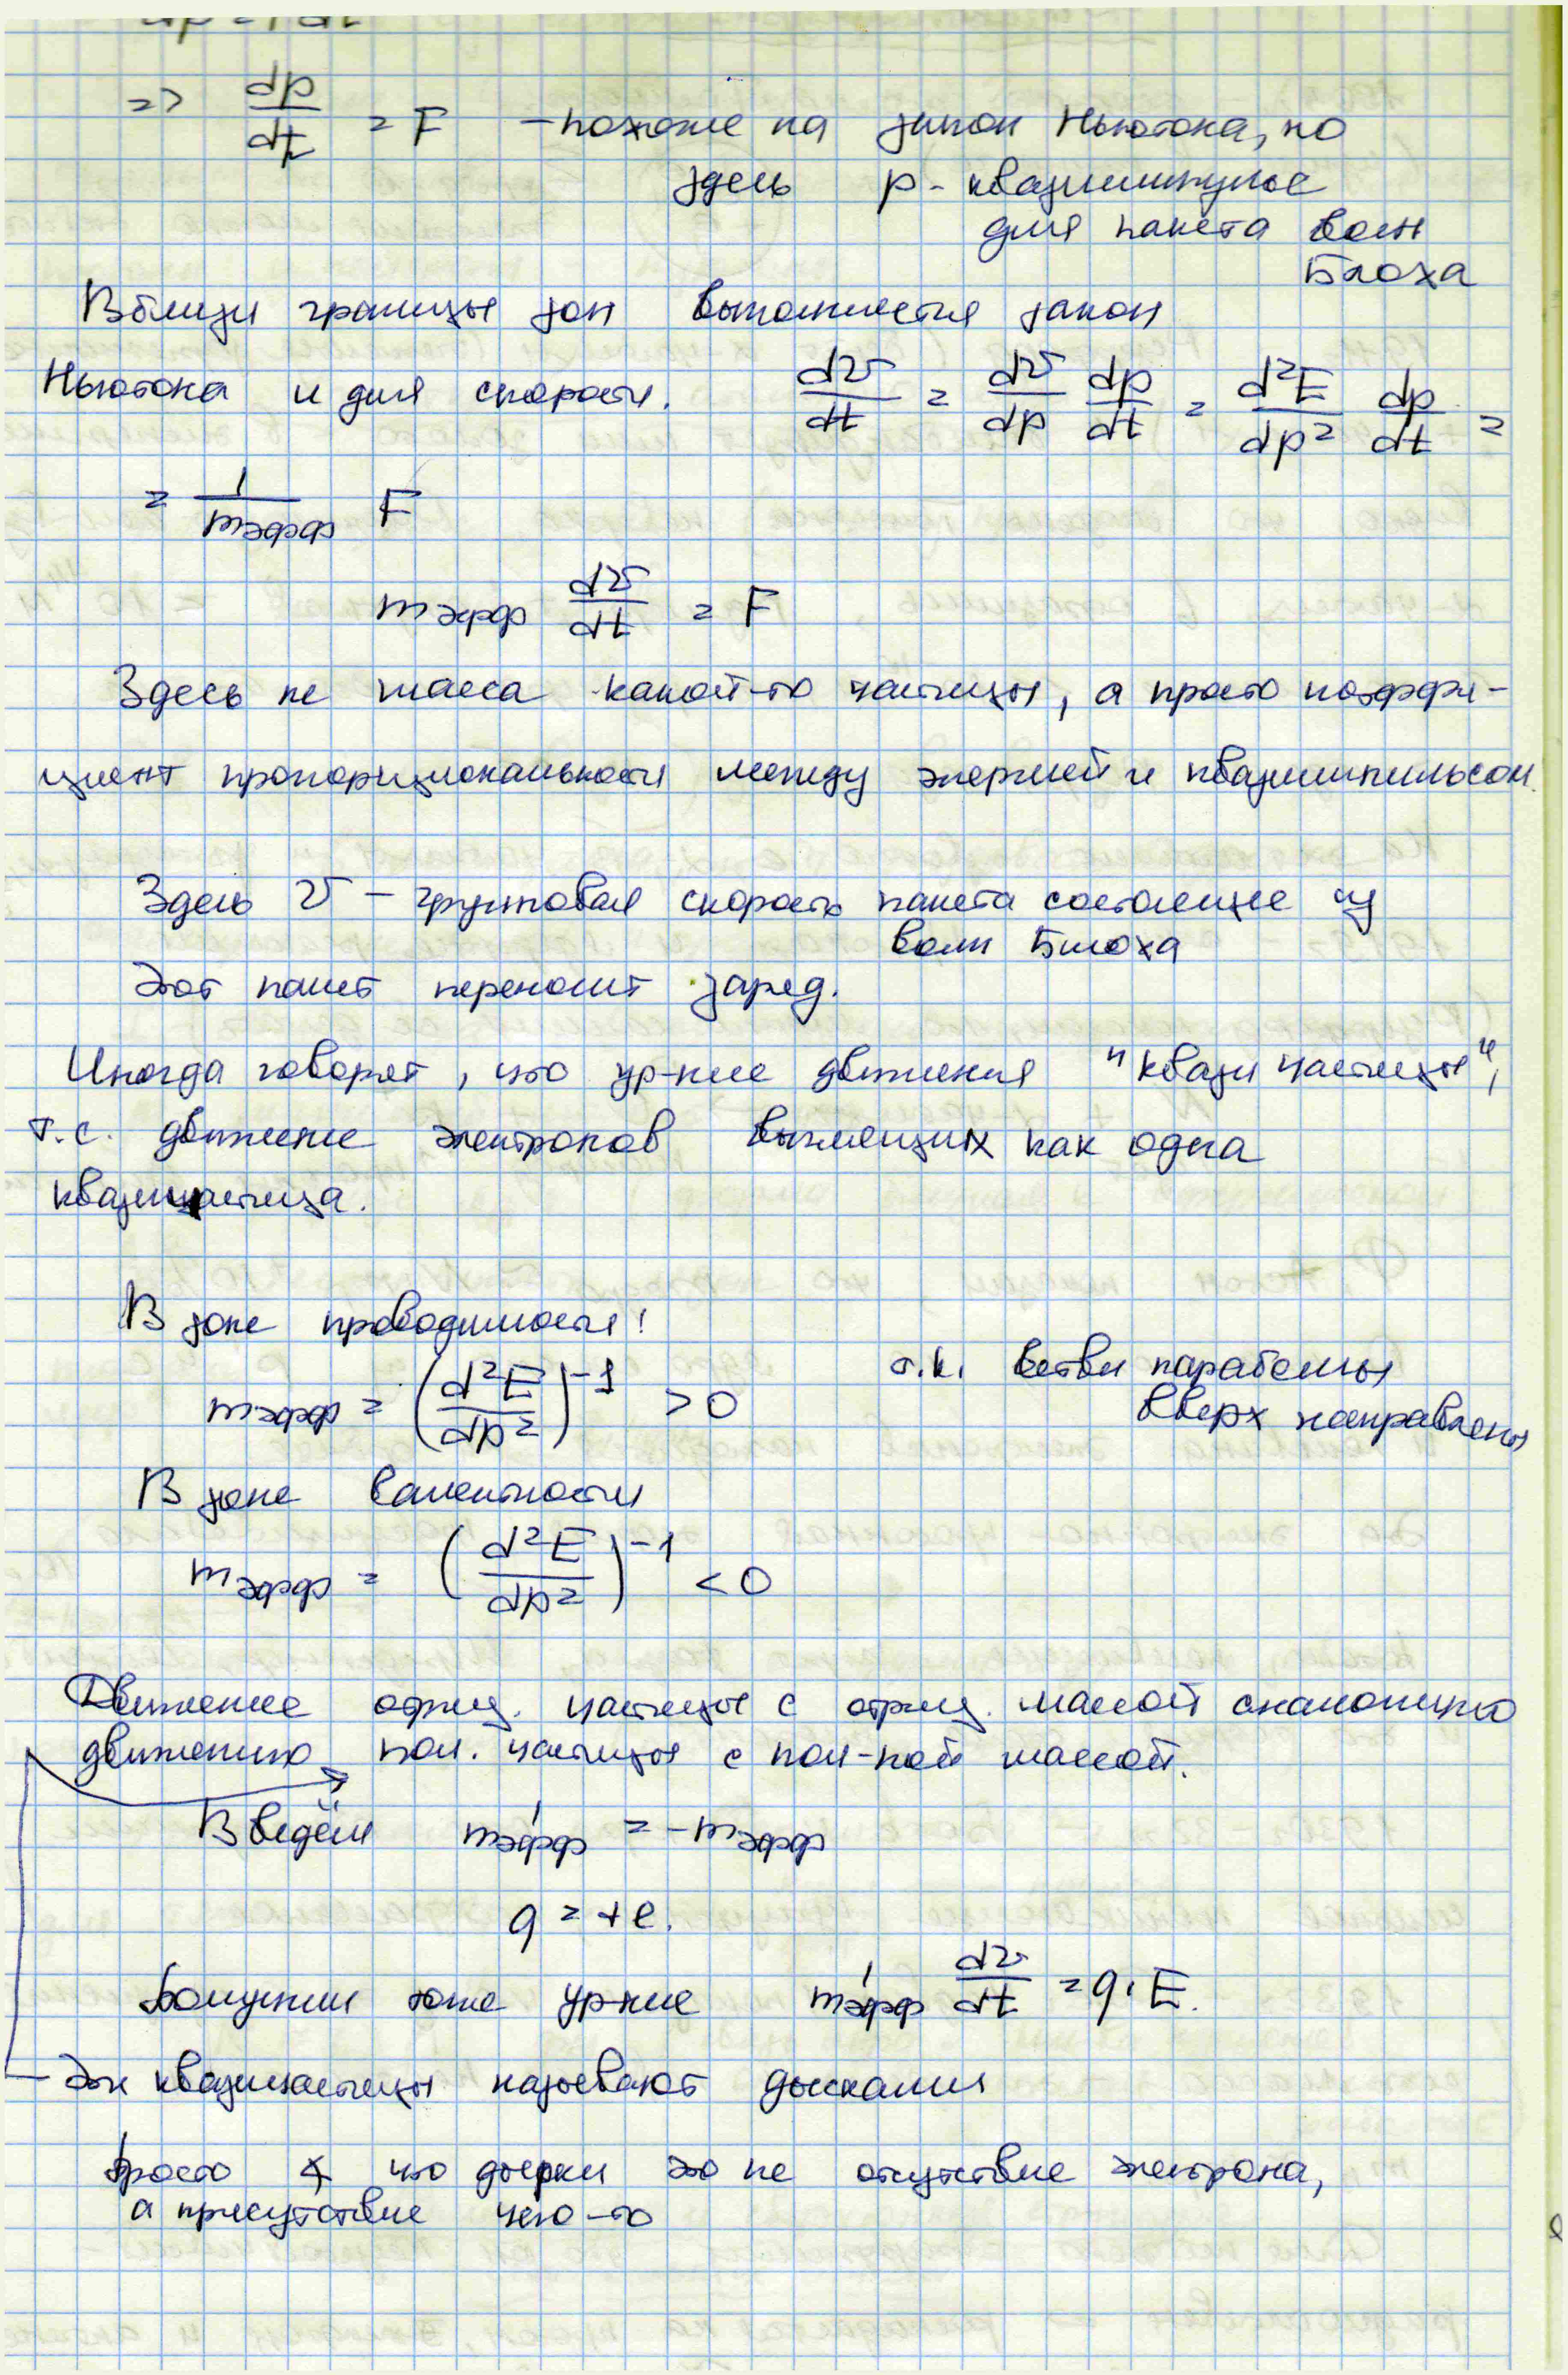
\includegraphics[max size={\textwidth}{0.995\textheight}]{jpg/42.jpg}%
\newpage%
%
%
\phantomsection\addcontentsline{toc}{part}{\textit{Физика атомного ядра и элементарных частиц}}%
\phantomsection\addcontentsline{toc}{section}{Физика атомного ядра}%
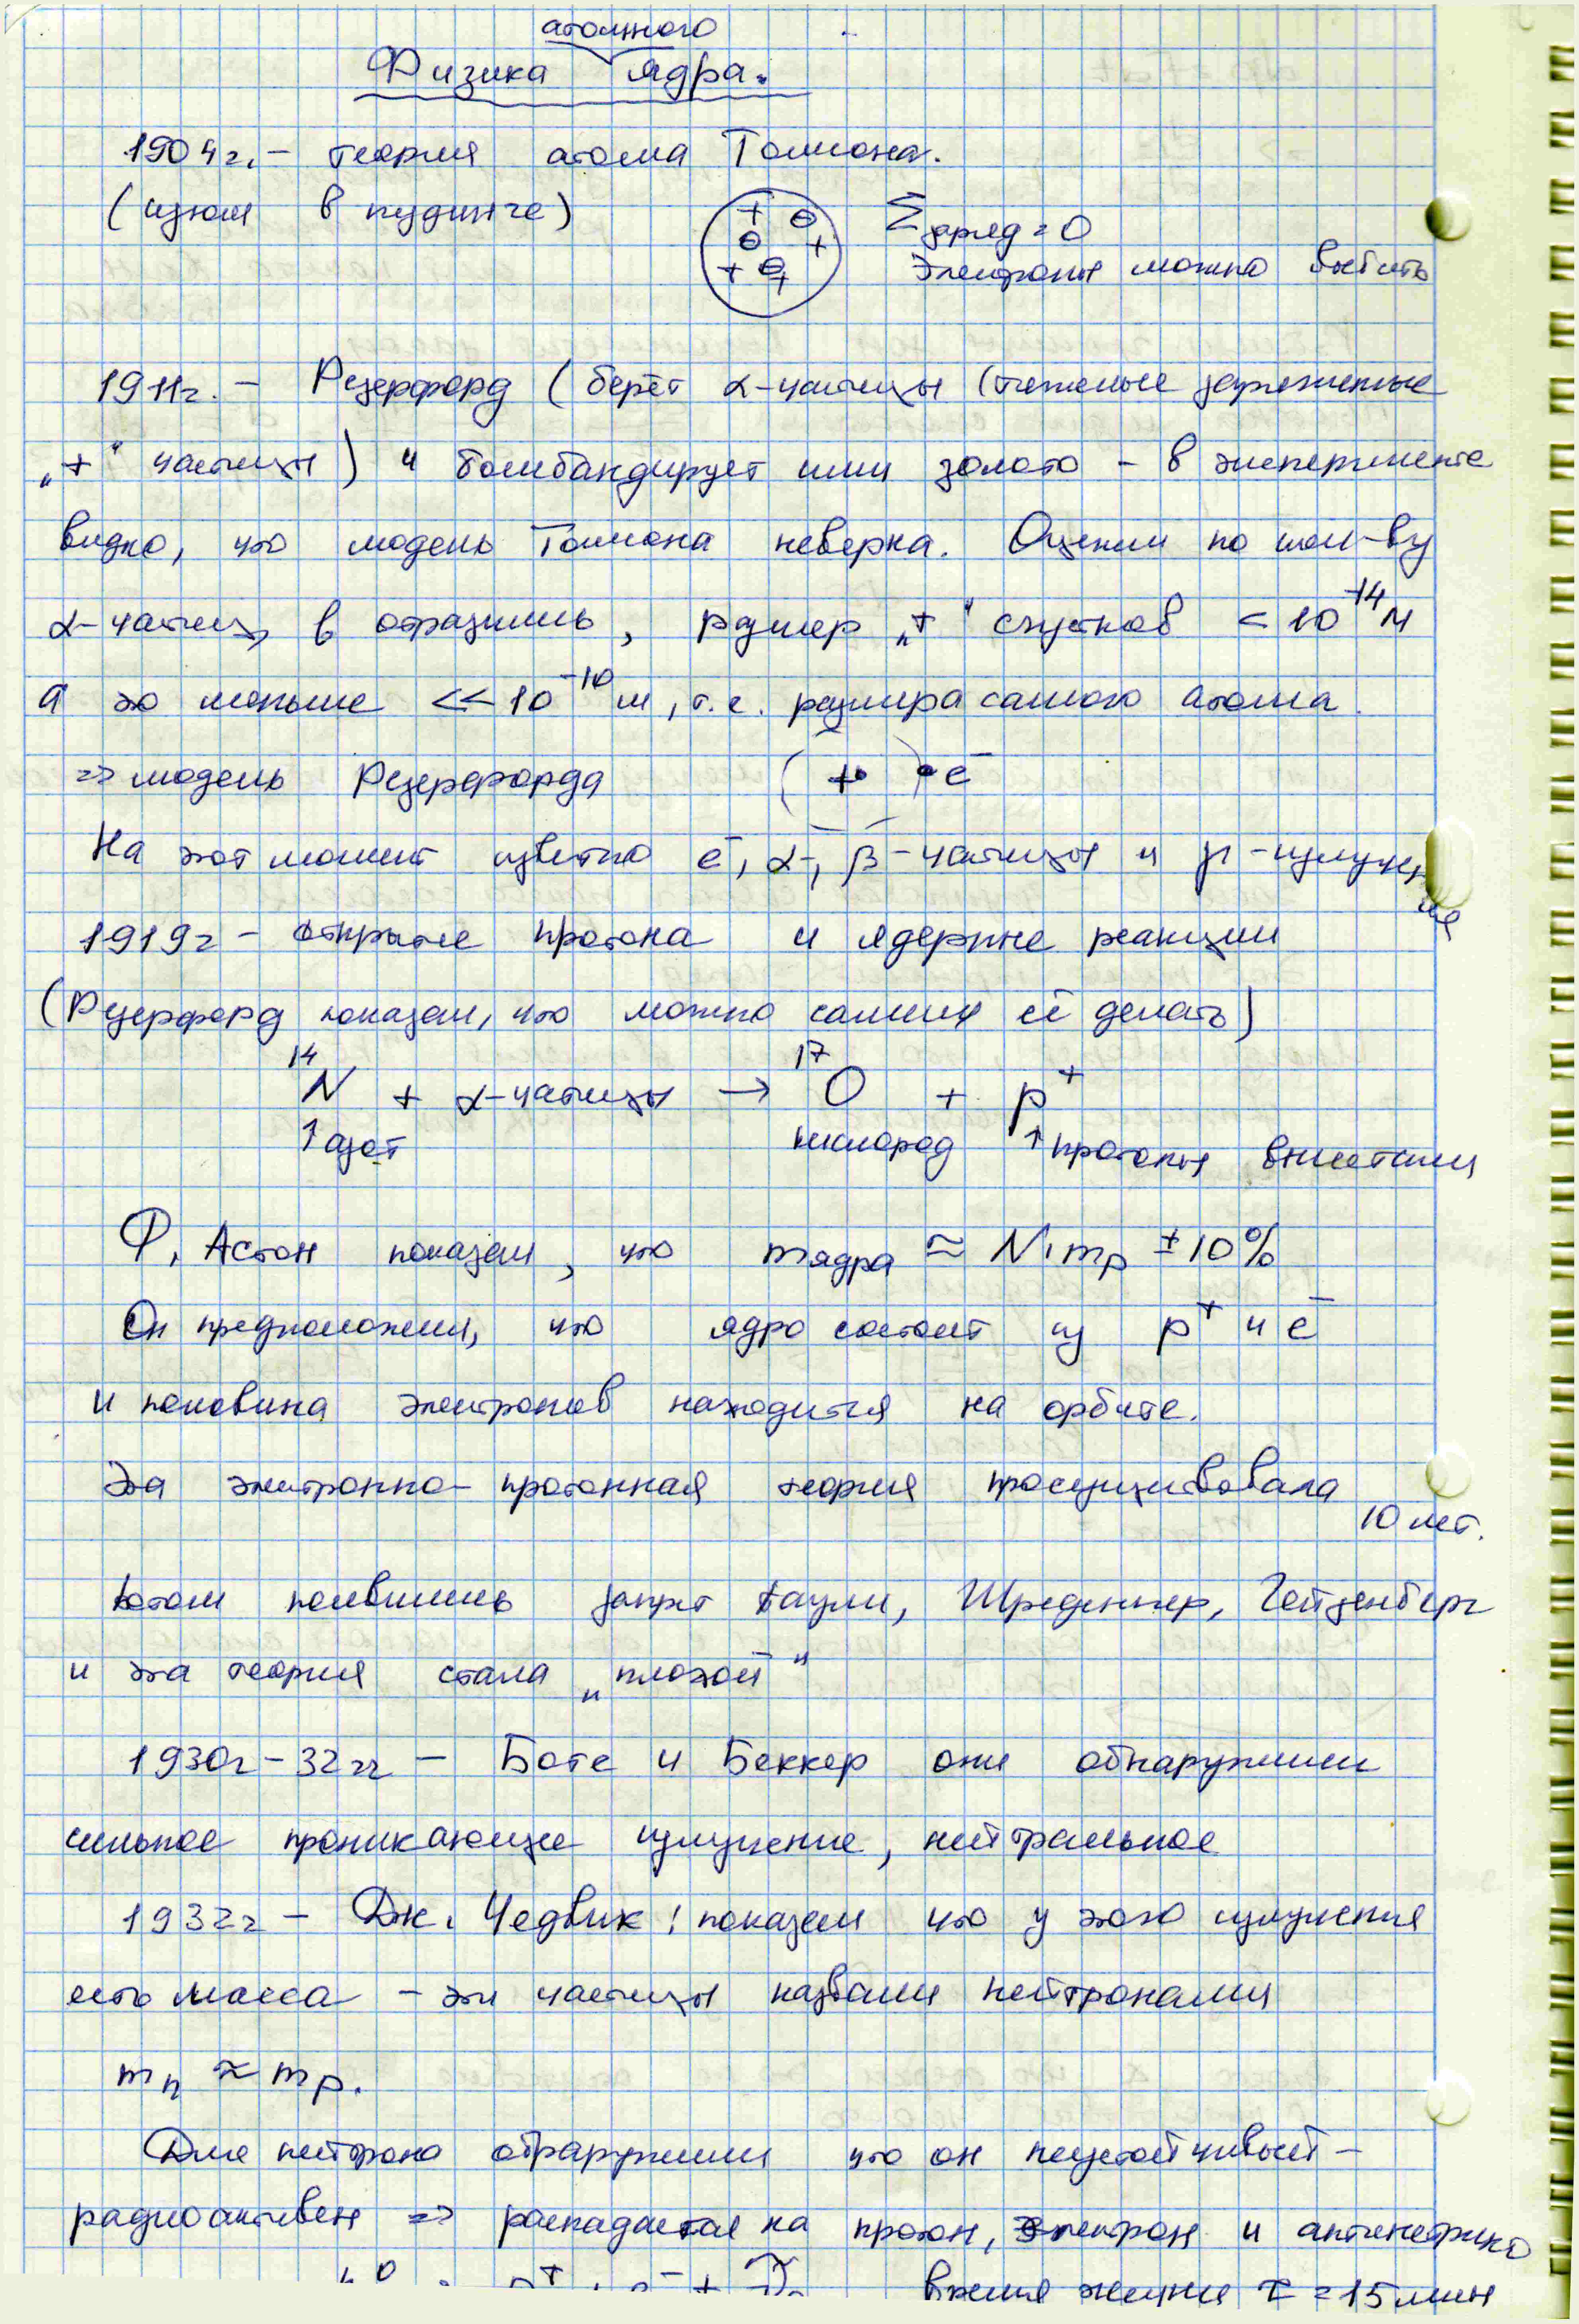
\includegraphics[max size={\textwidth}{0.995\textheight}]{jpg/43.jpg}%
\newpage%
%
%
\phantomsection\addcontentsline{toc}{subsection}{Характеристики атомного ядра}%
\phantomsection\addcontentsline{toc}{subsection}{Спин ядра и сверхтонкая структура спектральных линий}%
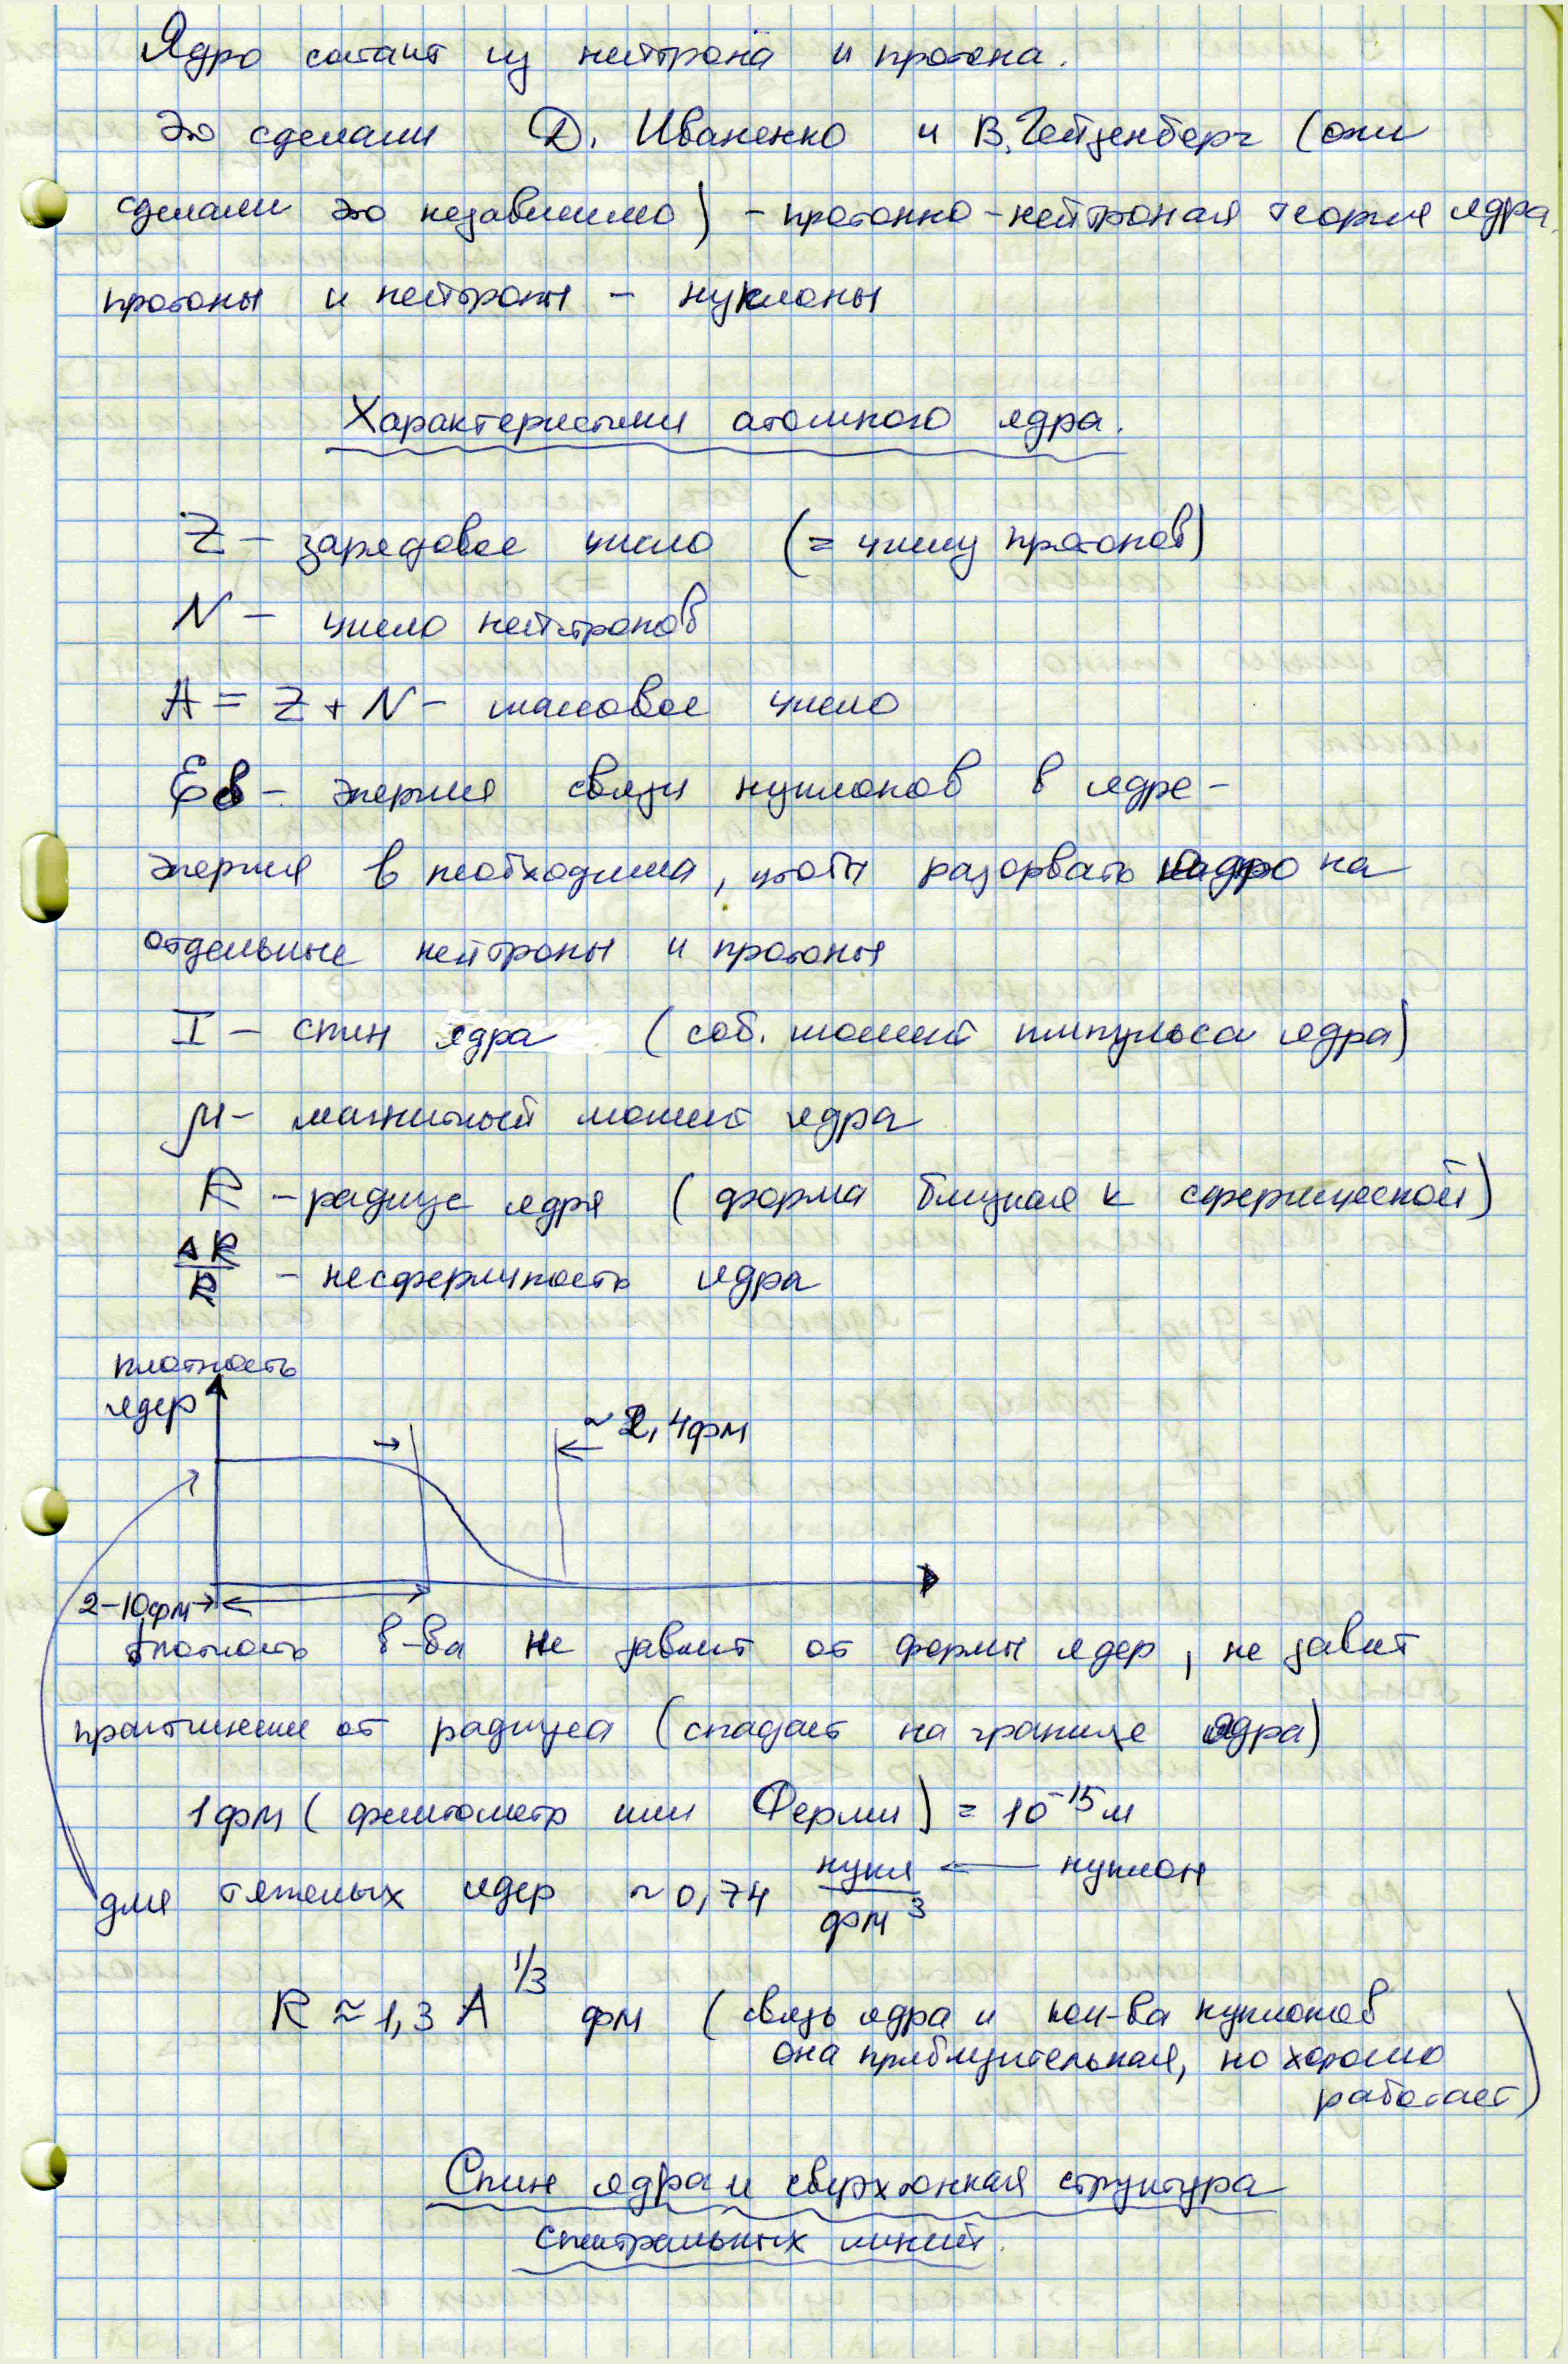
\includegraphics[max size={\textwidth}{0.995\textheight}]{jpg/44.jpg}%
\newpage%
%
%
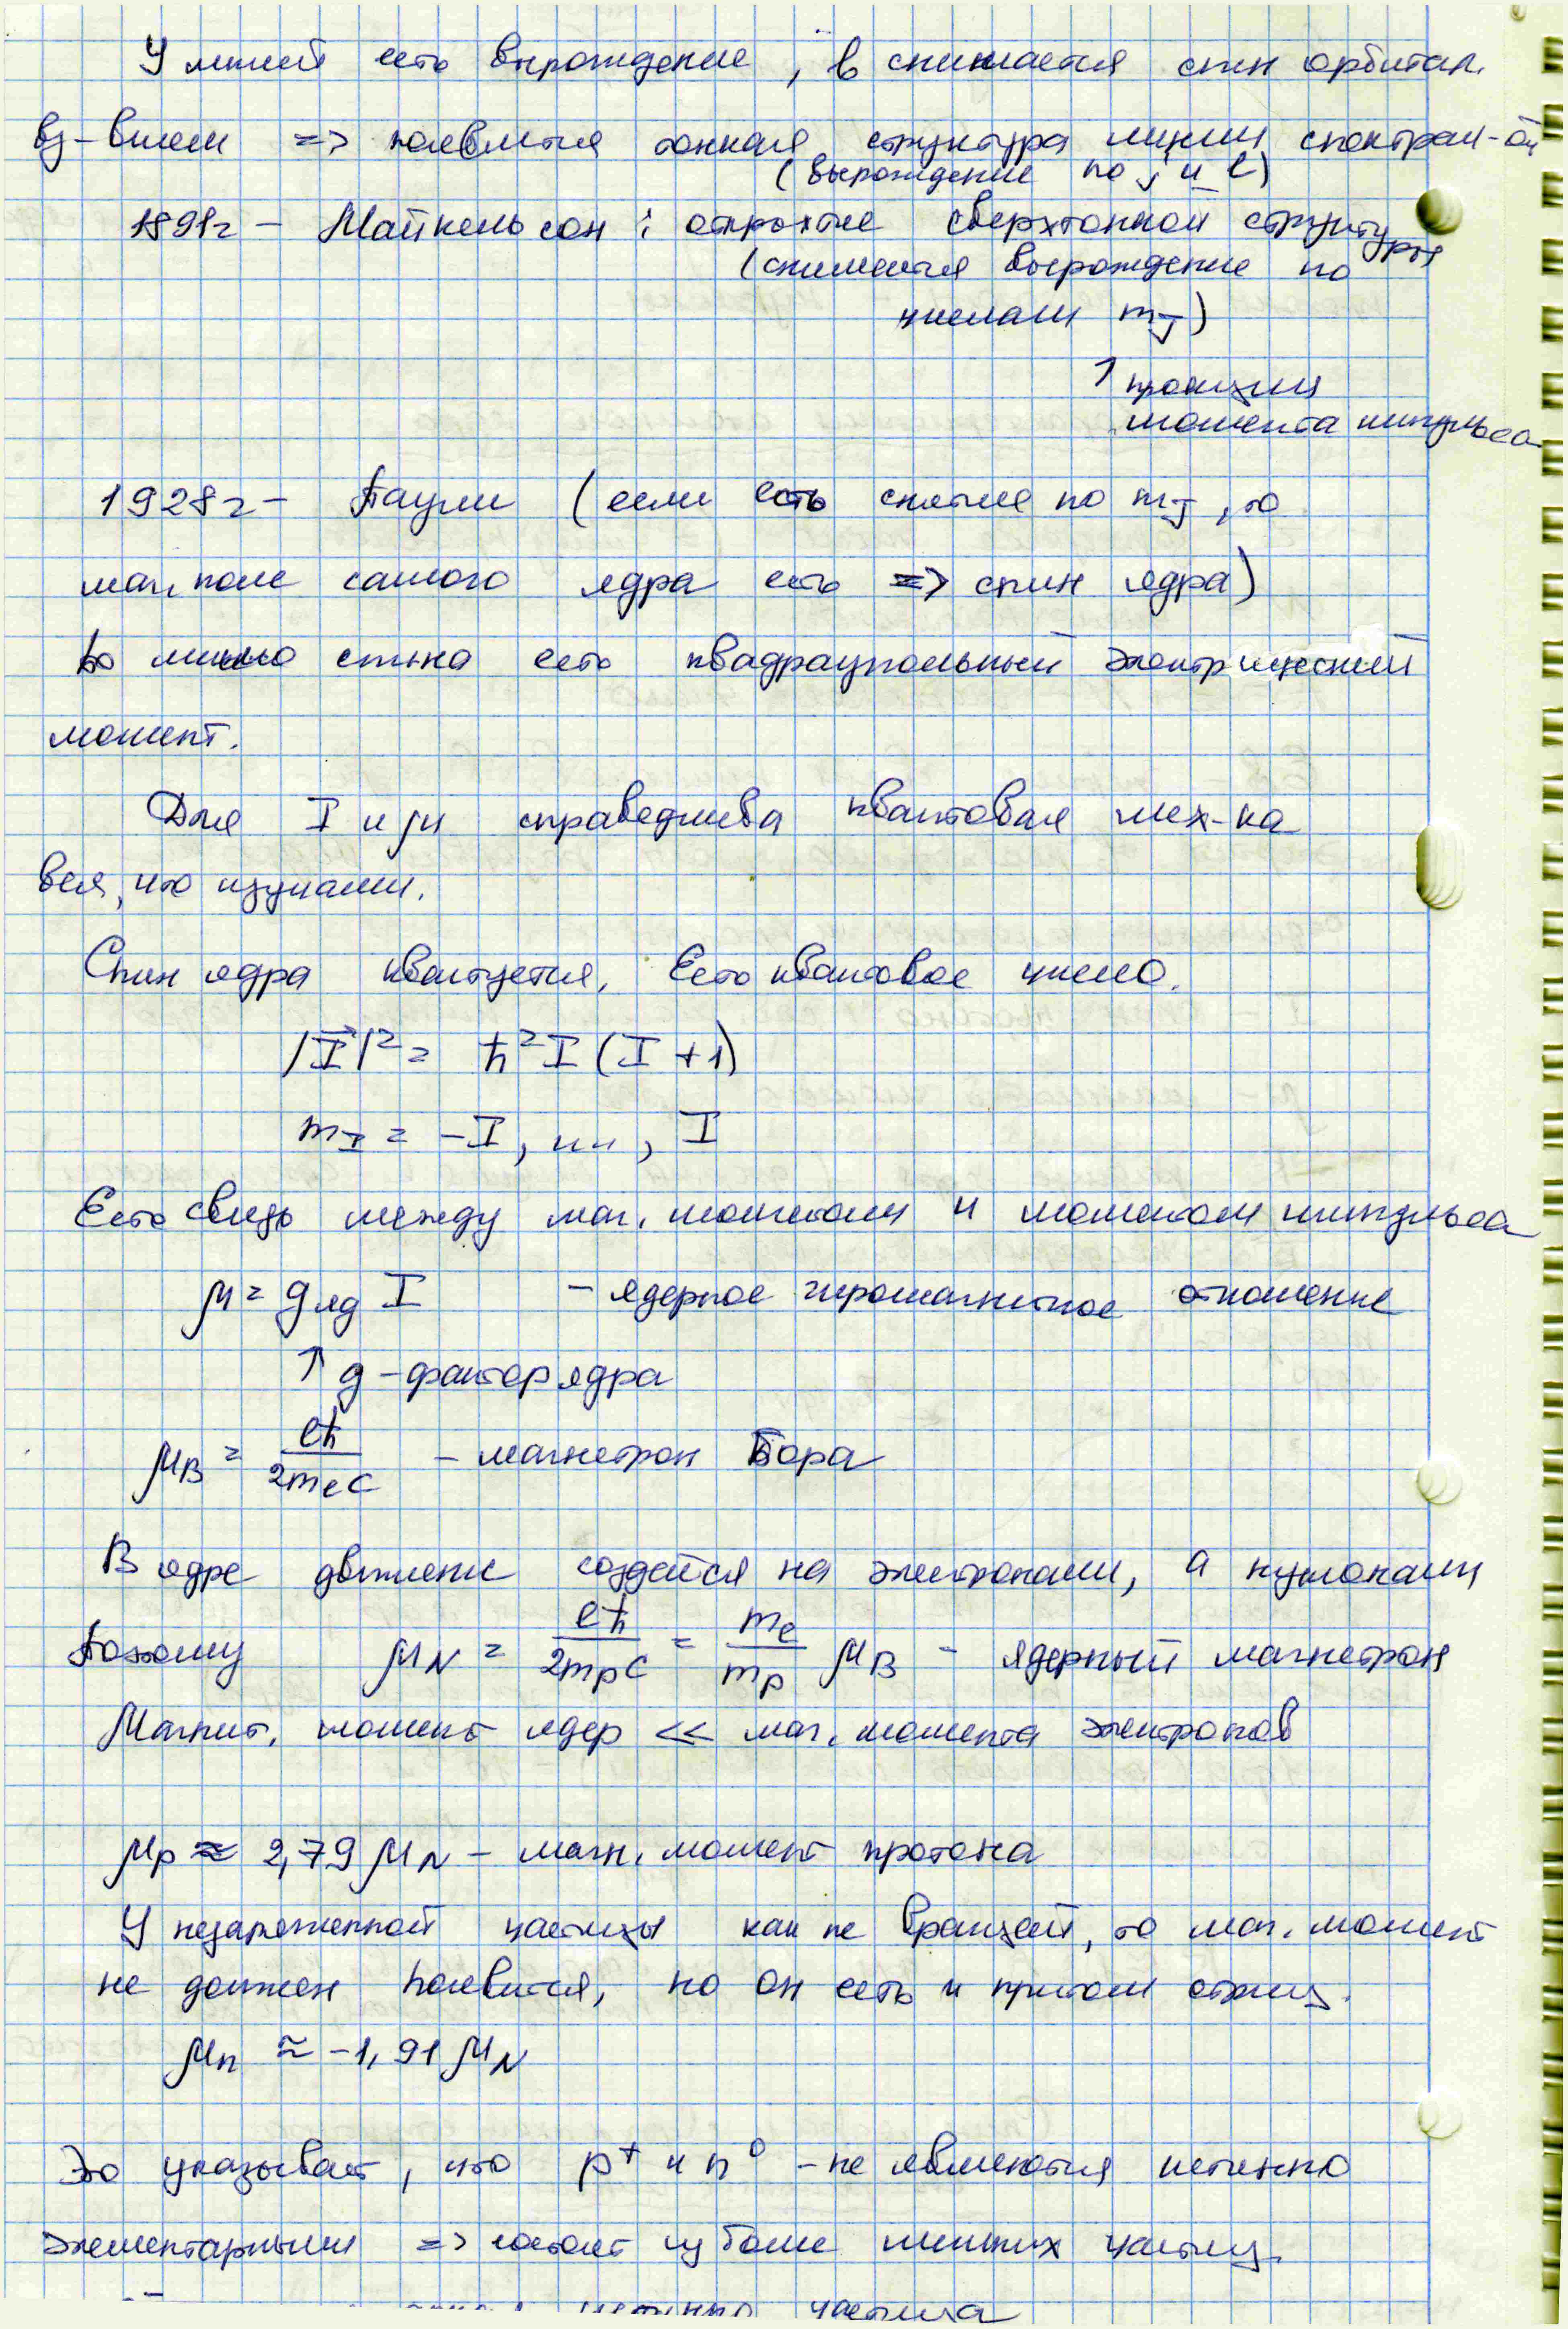
\includegraphics[max size={\textwidth}{0.995\textheight}]{jpg/45.jpg}%
\newpage%
%
%
\phantomsection\addcontentsline{toc}{subsection}{Масса ядра и энергия связи нуклонов в ядре}%
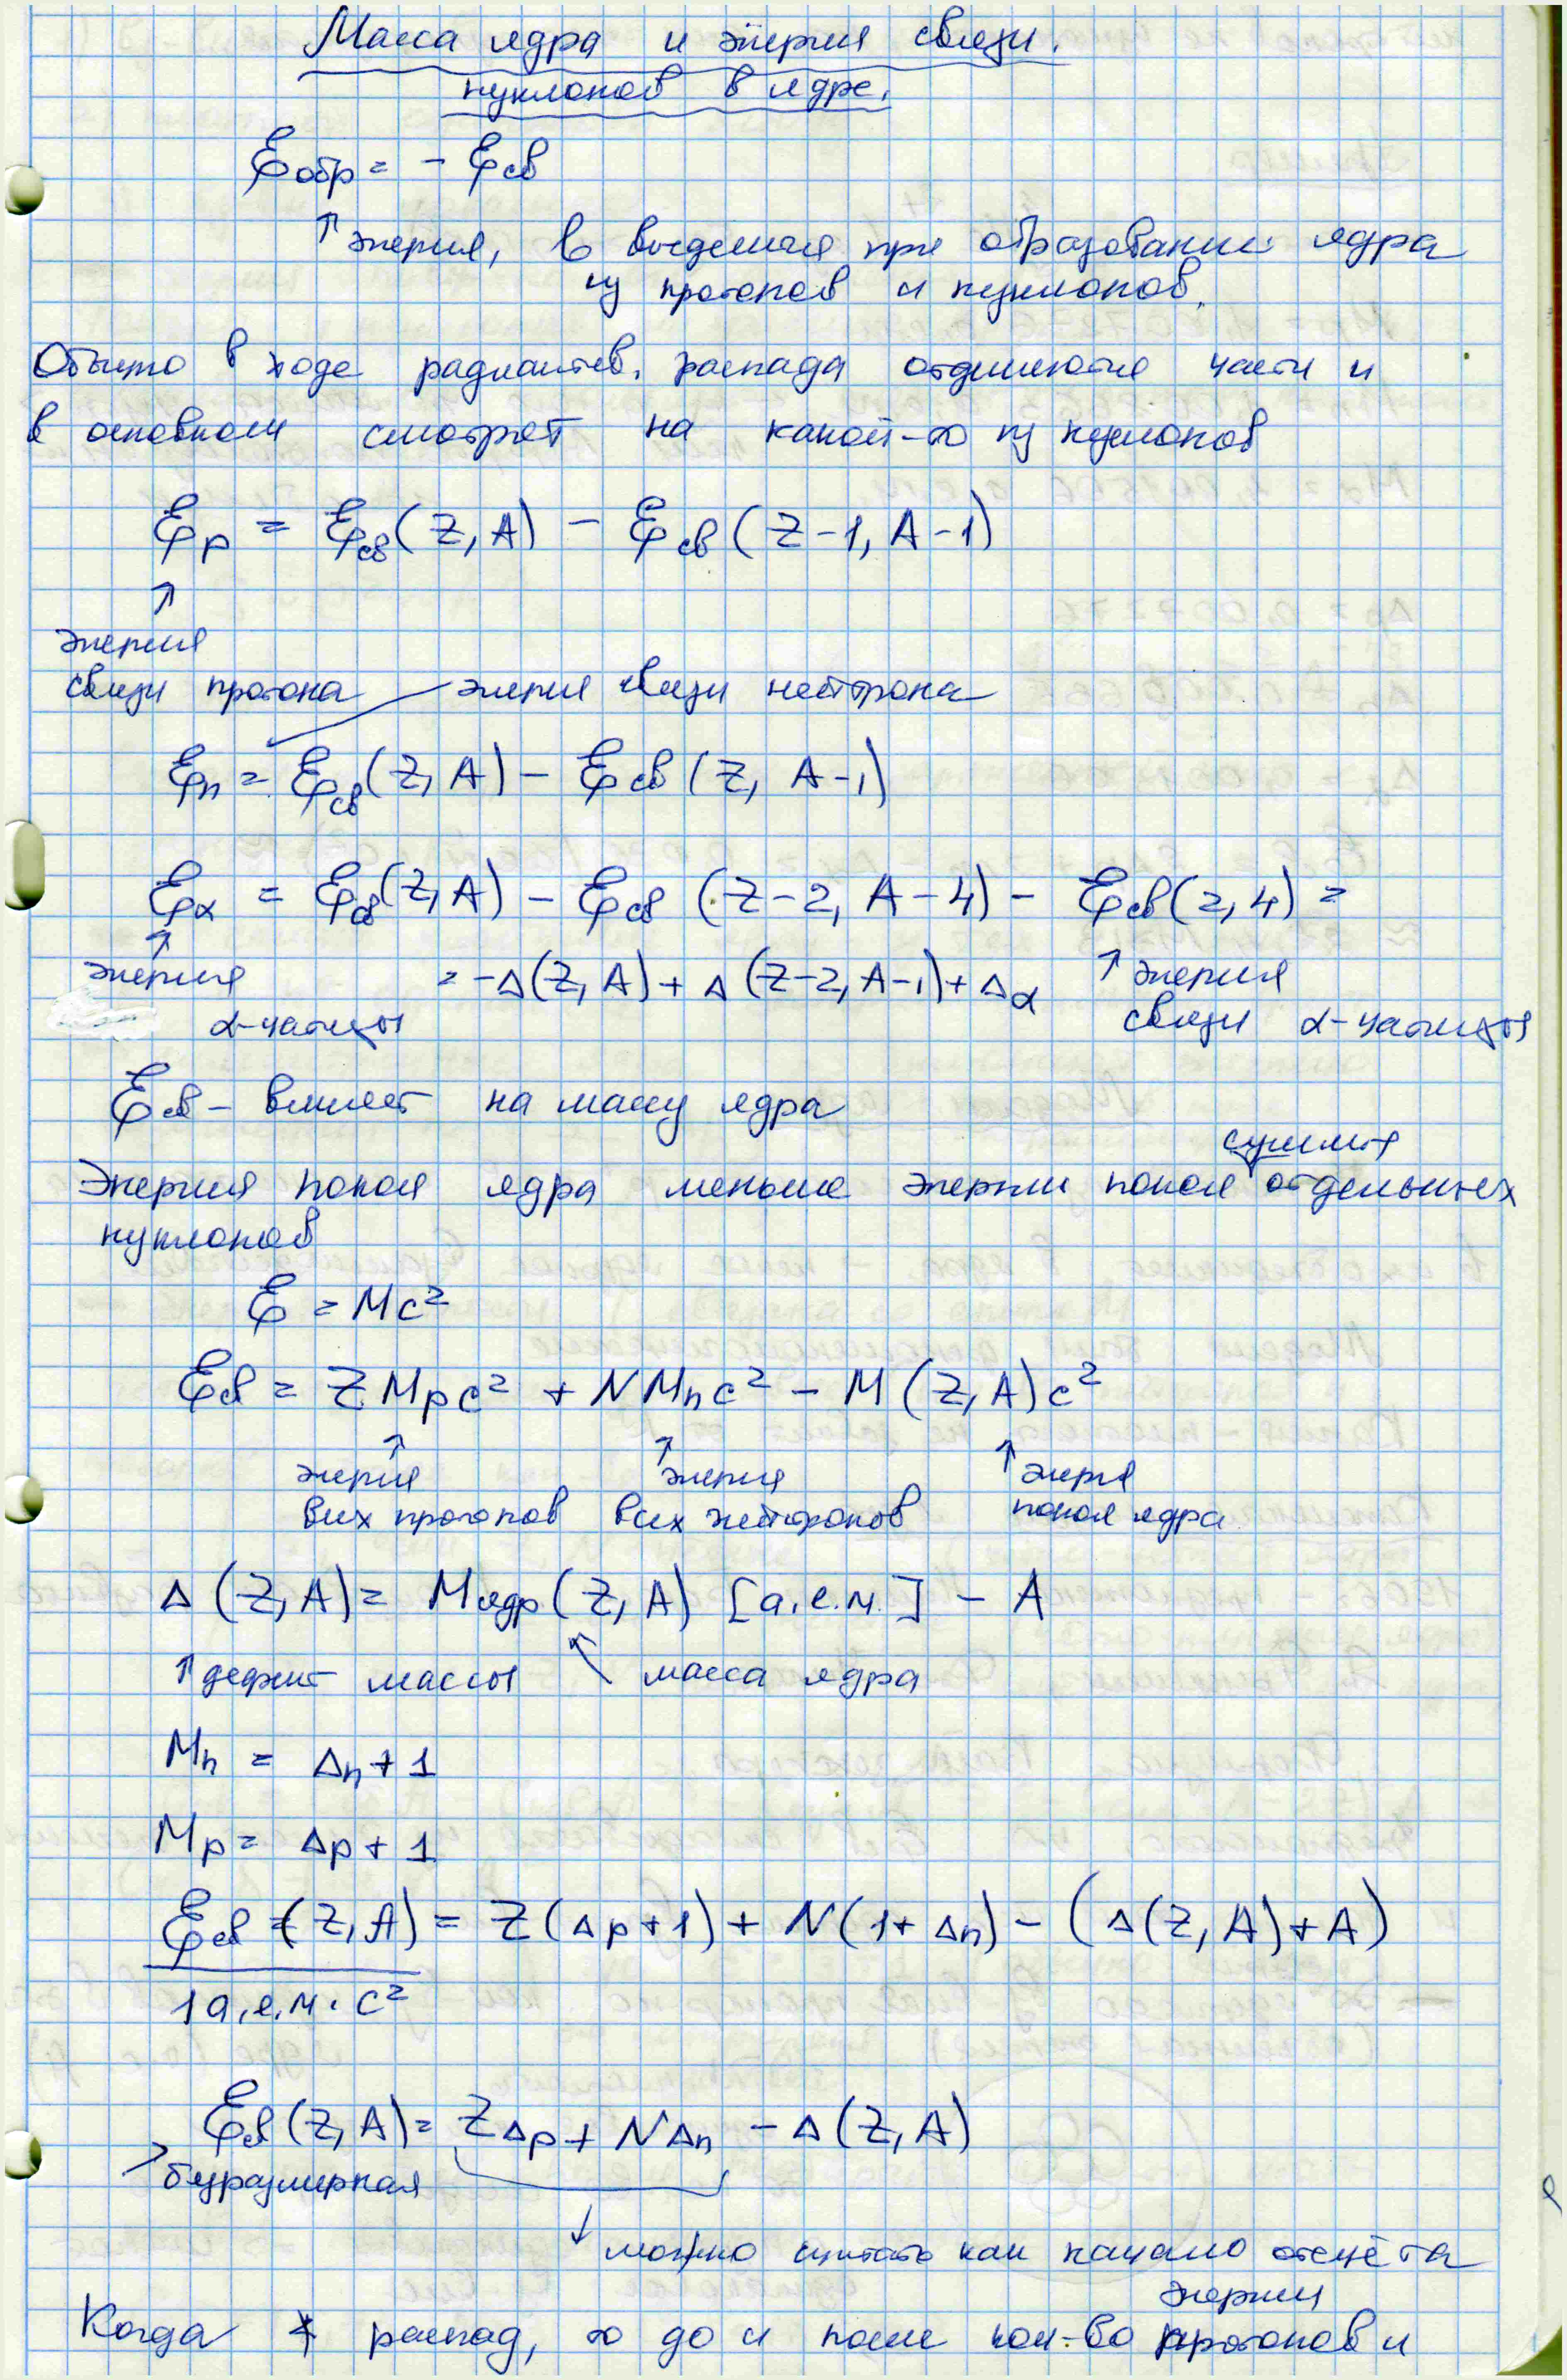
\includegraphics[max size={\textwidth}{0.995\textheight}]{jpg/46.jpg}%
\newpage%
%
%
\phantomsection\addcontentsline{toc}{subsection}{Модели ядра}%
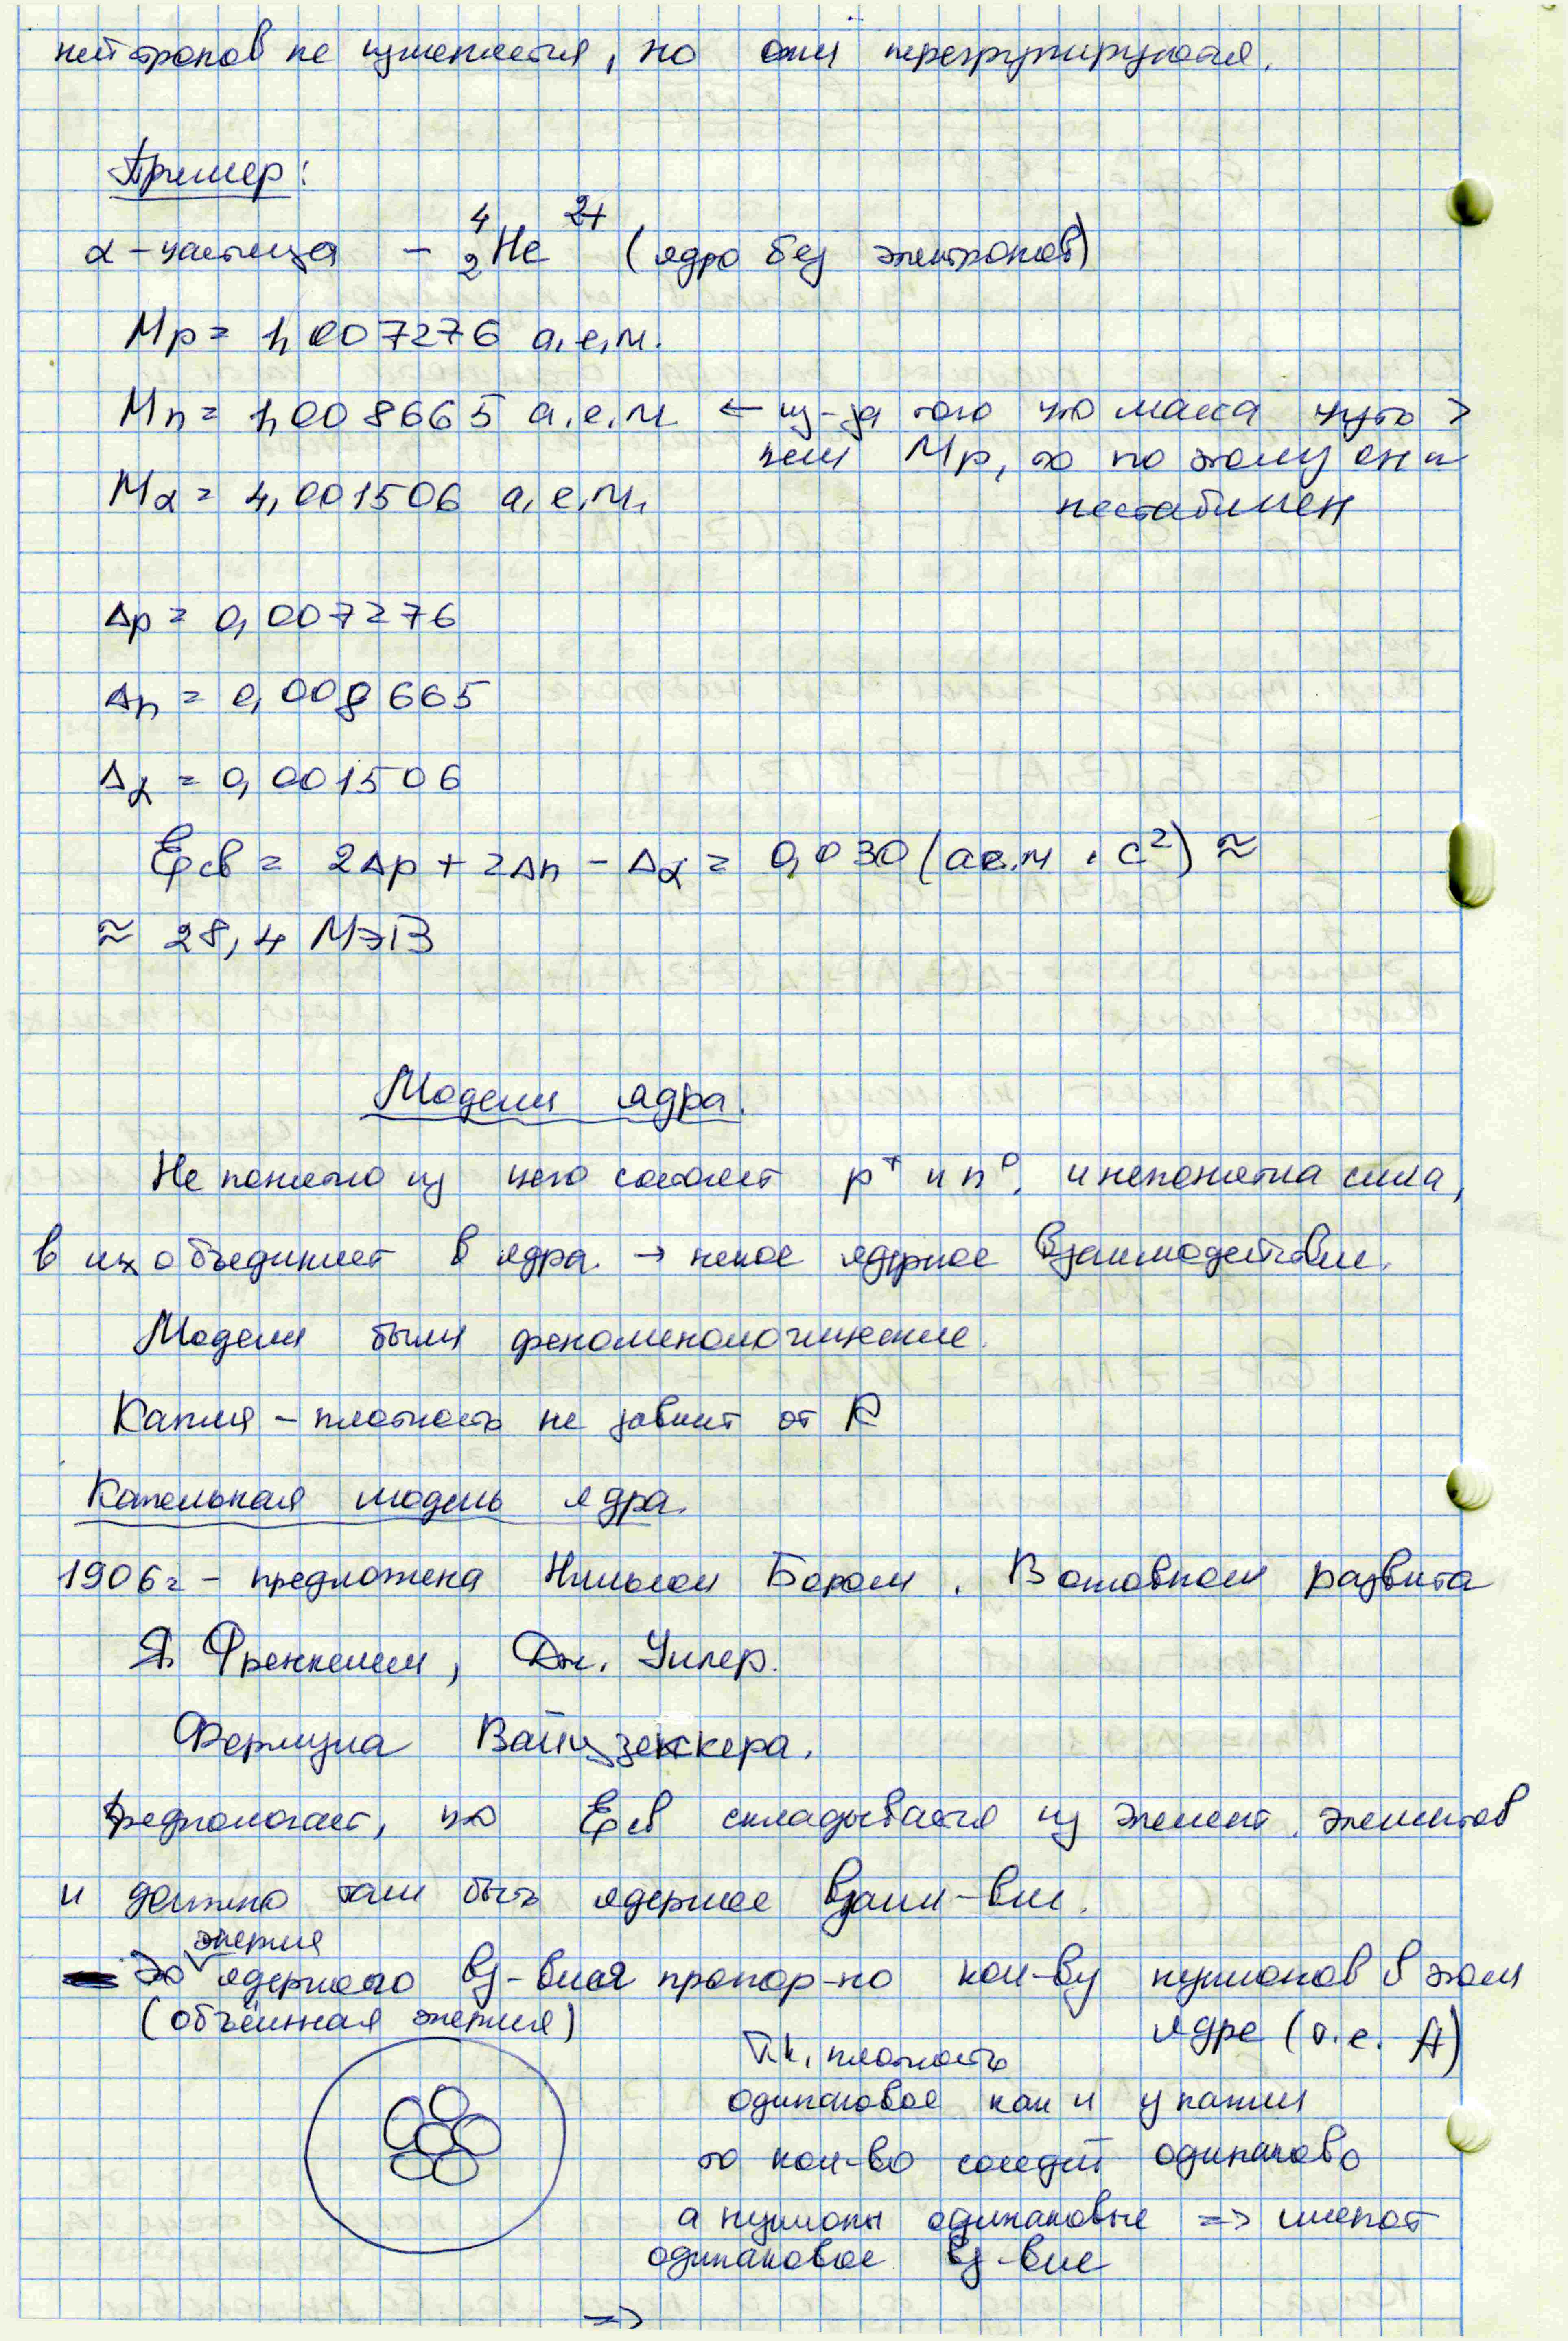
\includegraphics[max size={\textwidth}{0.995\textheight}]{jpg/47.jpg}%
\newpage%
%
%
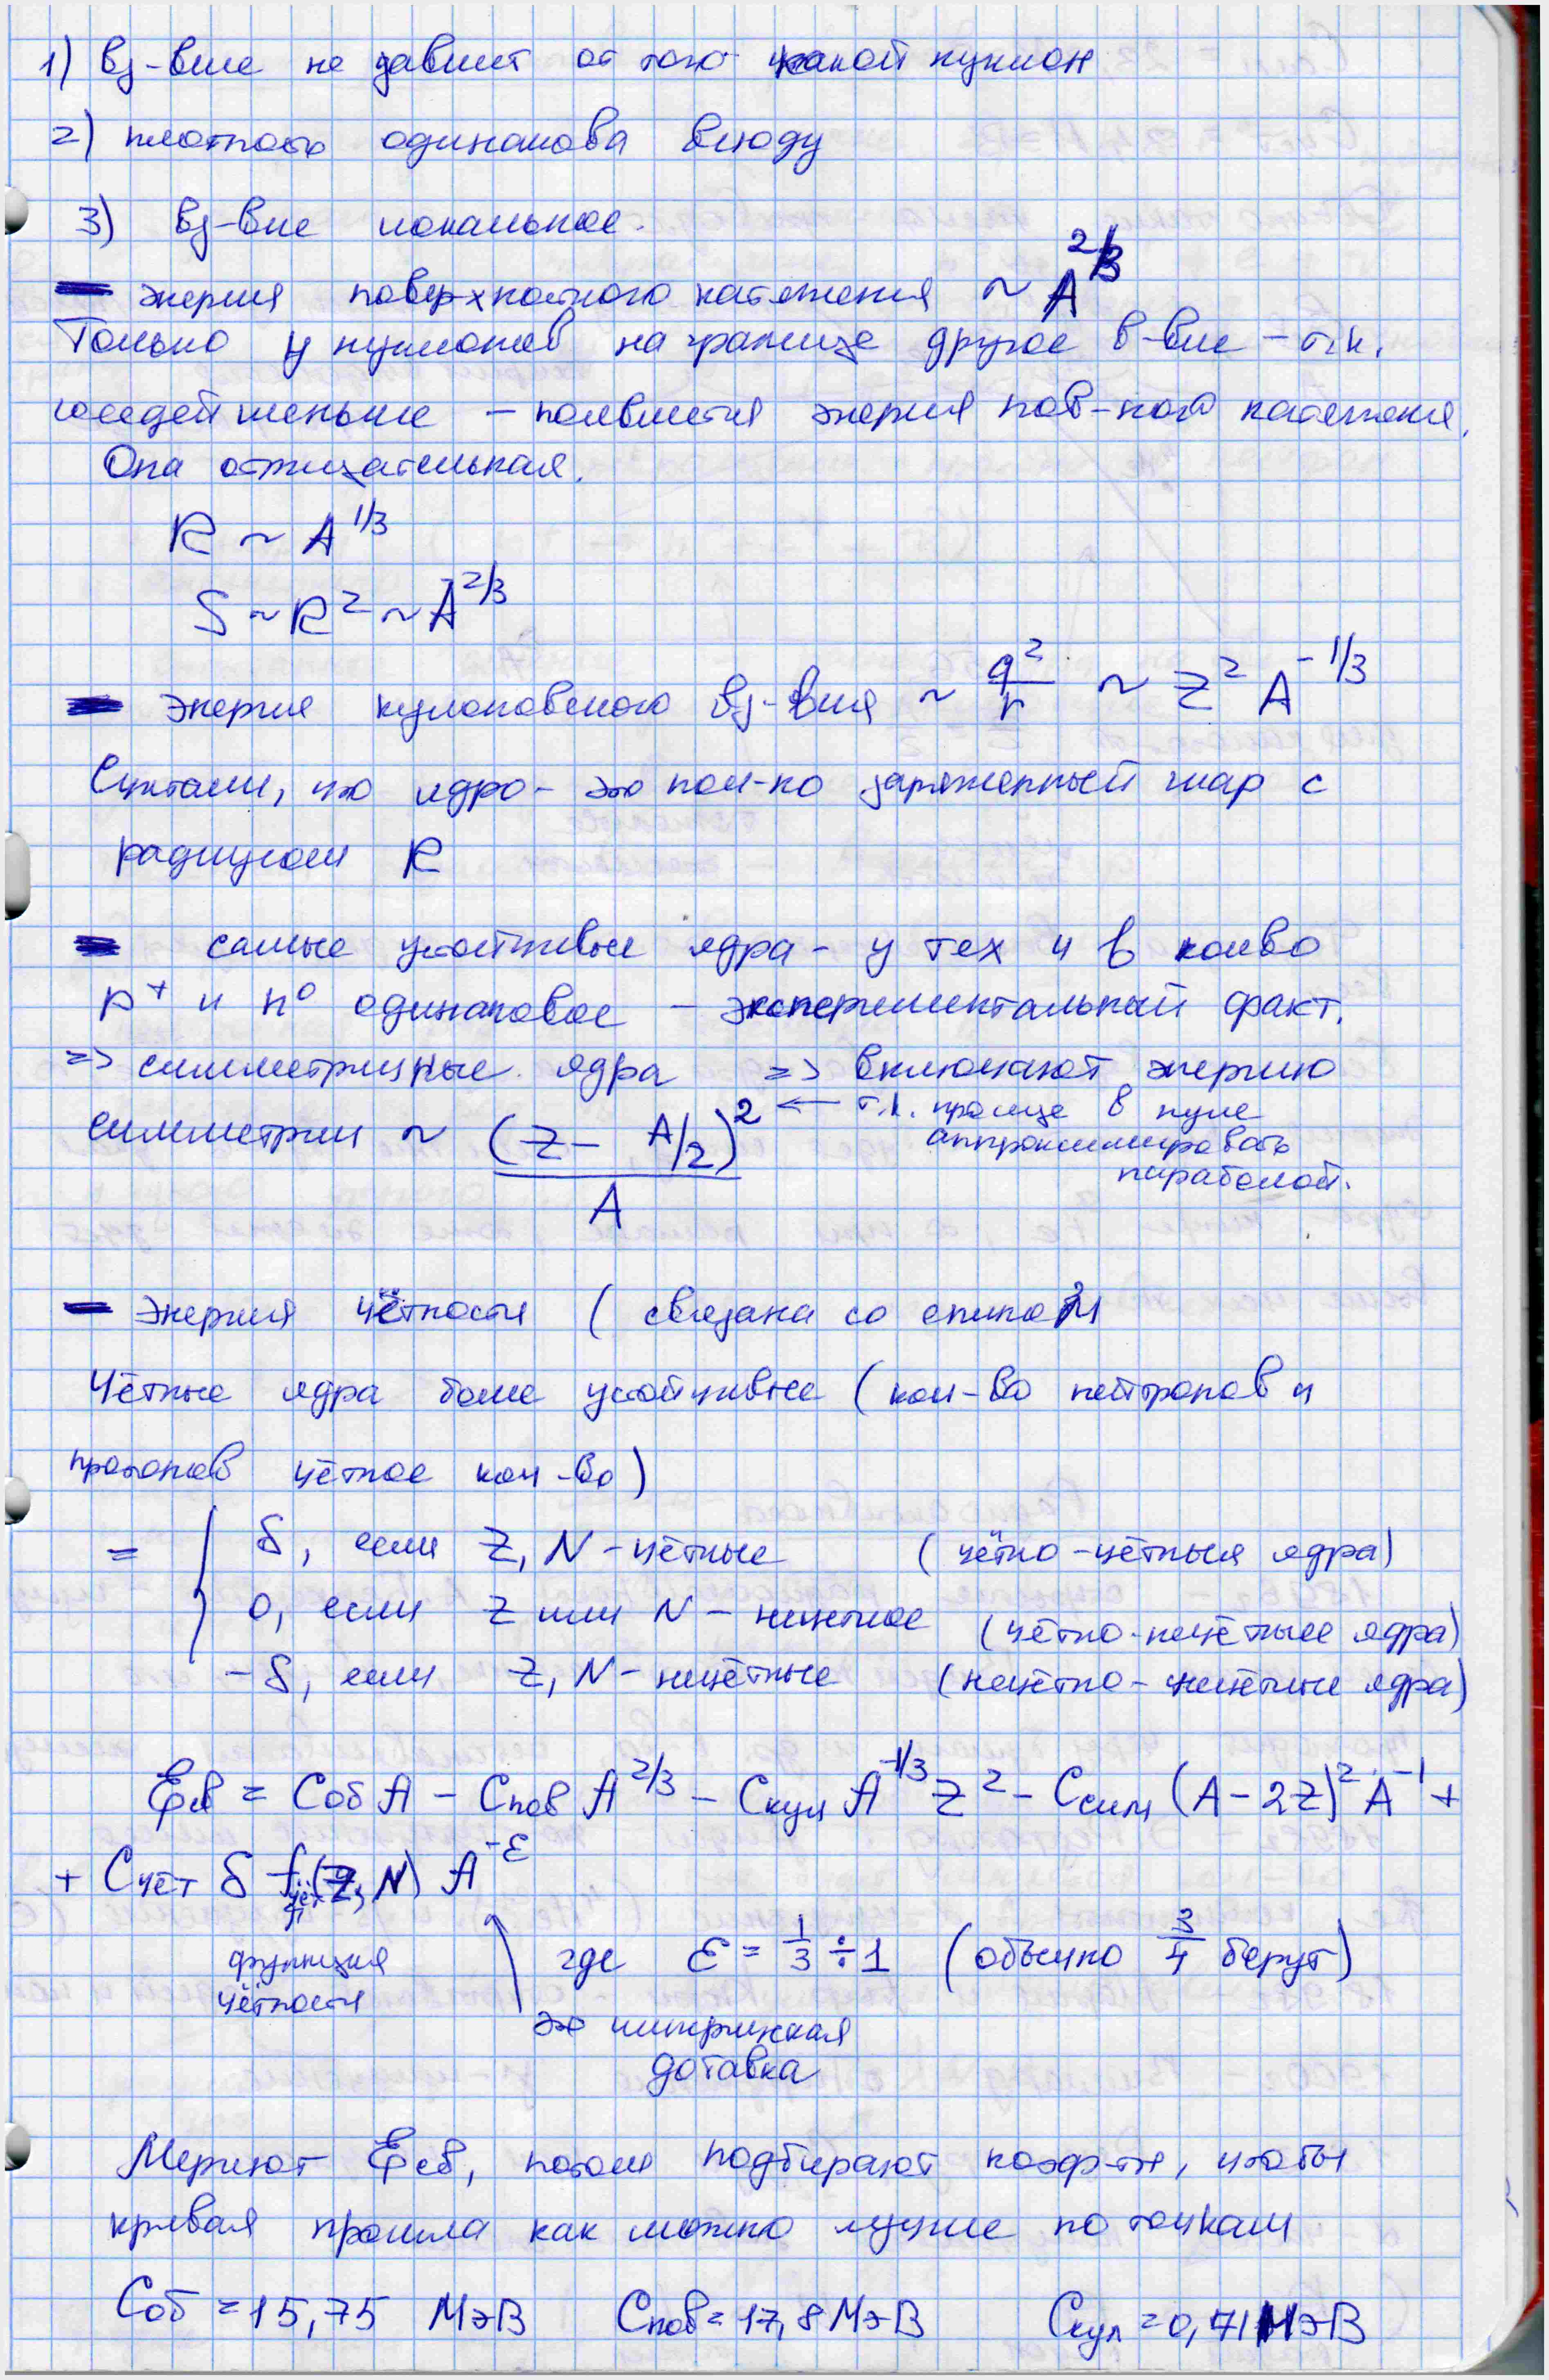
\includegraphics[max size={\textwidth}{0.995\textheight}]{jpg/48.jpg}%
\newpage%
%
\phantomsection\addcontentsline{toc}{subsection}{Радиоактивность}%
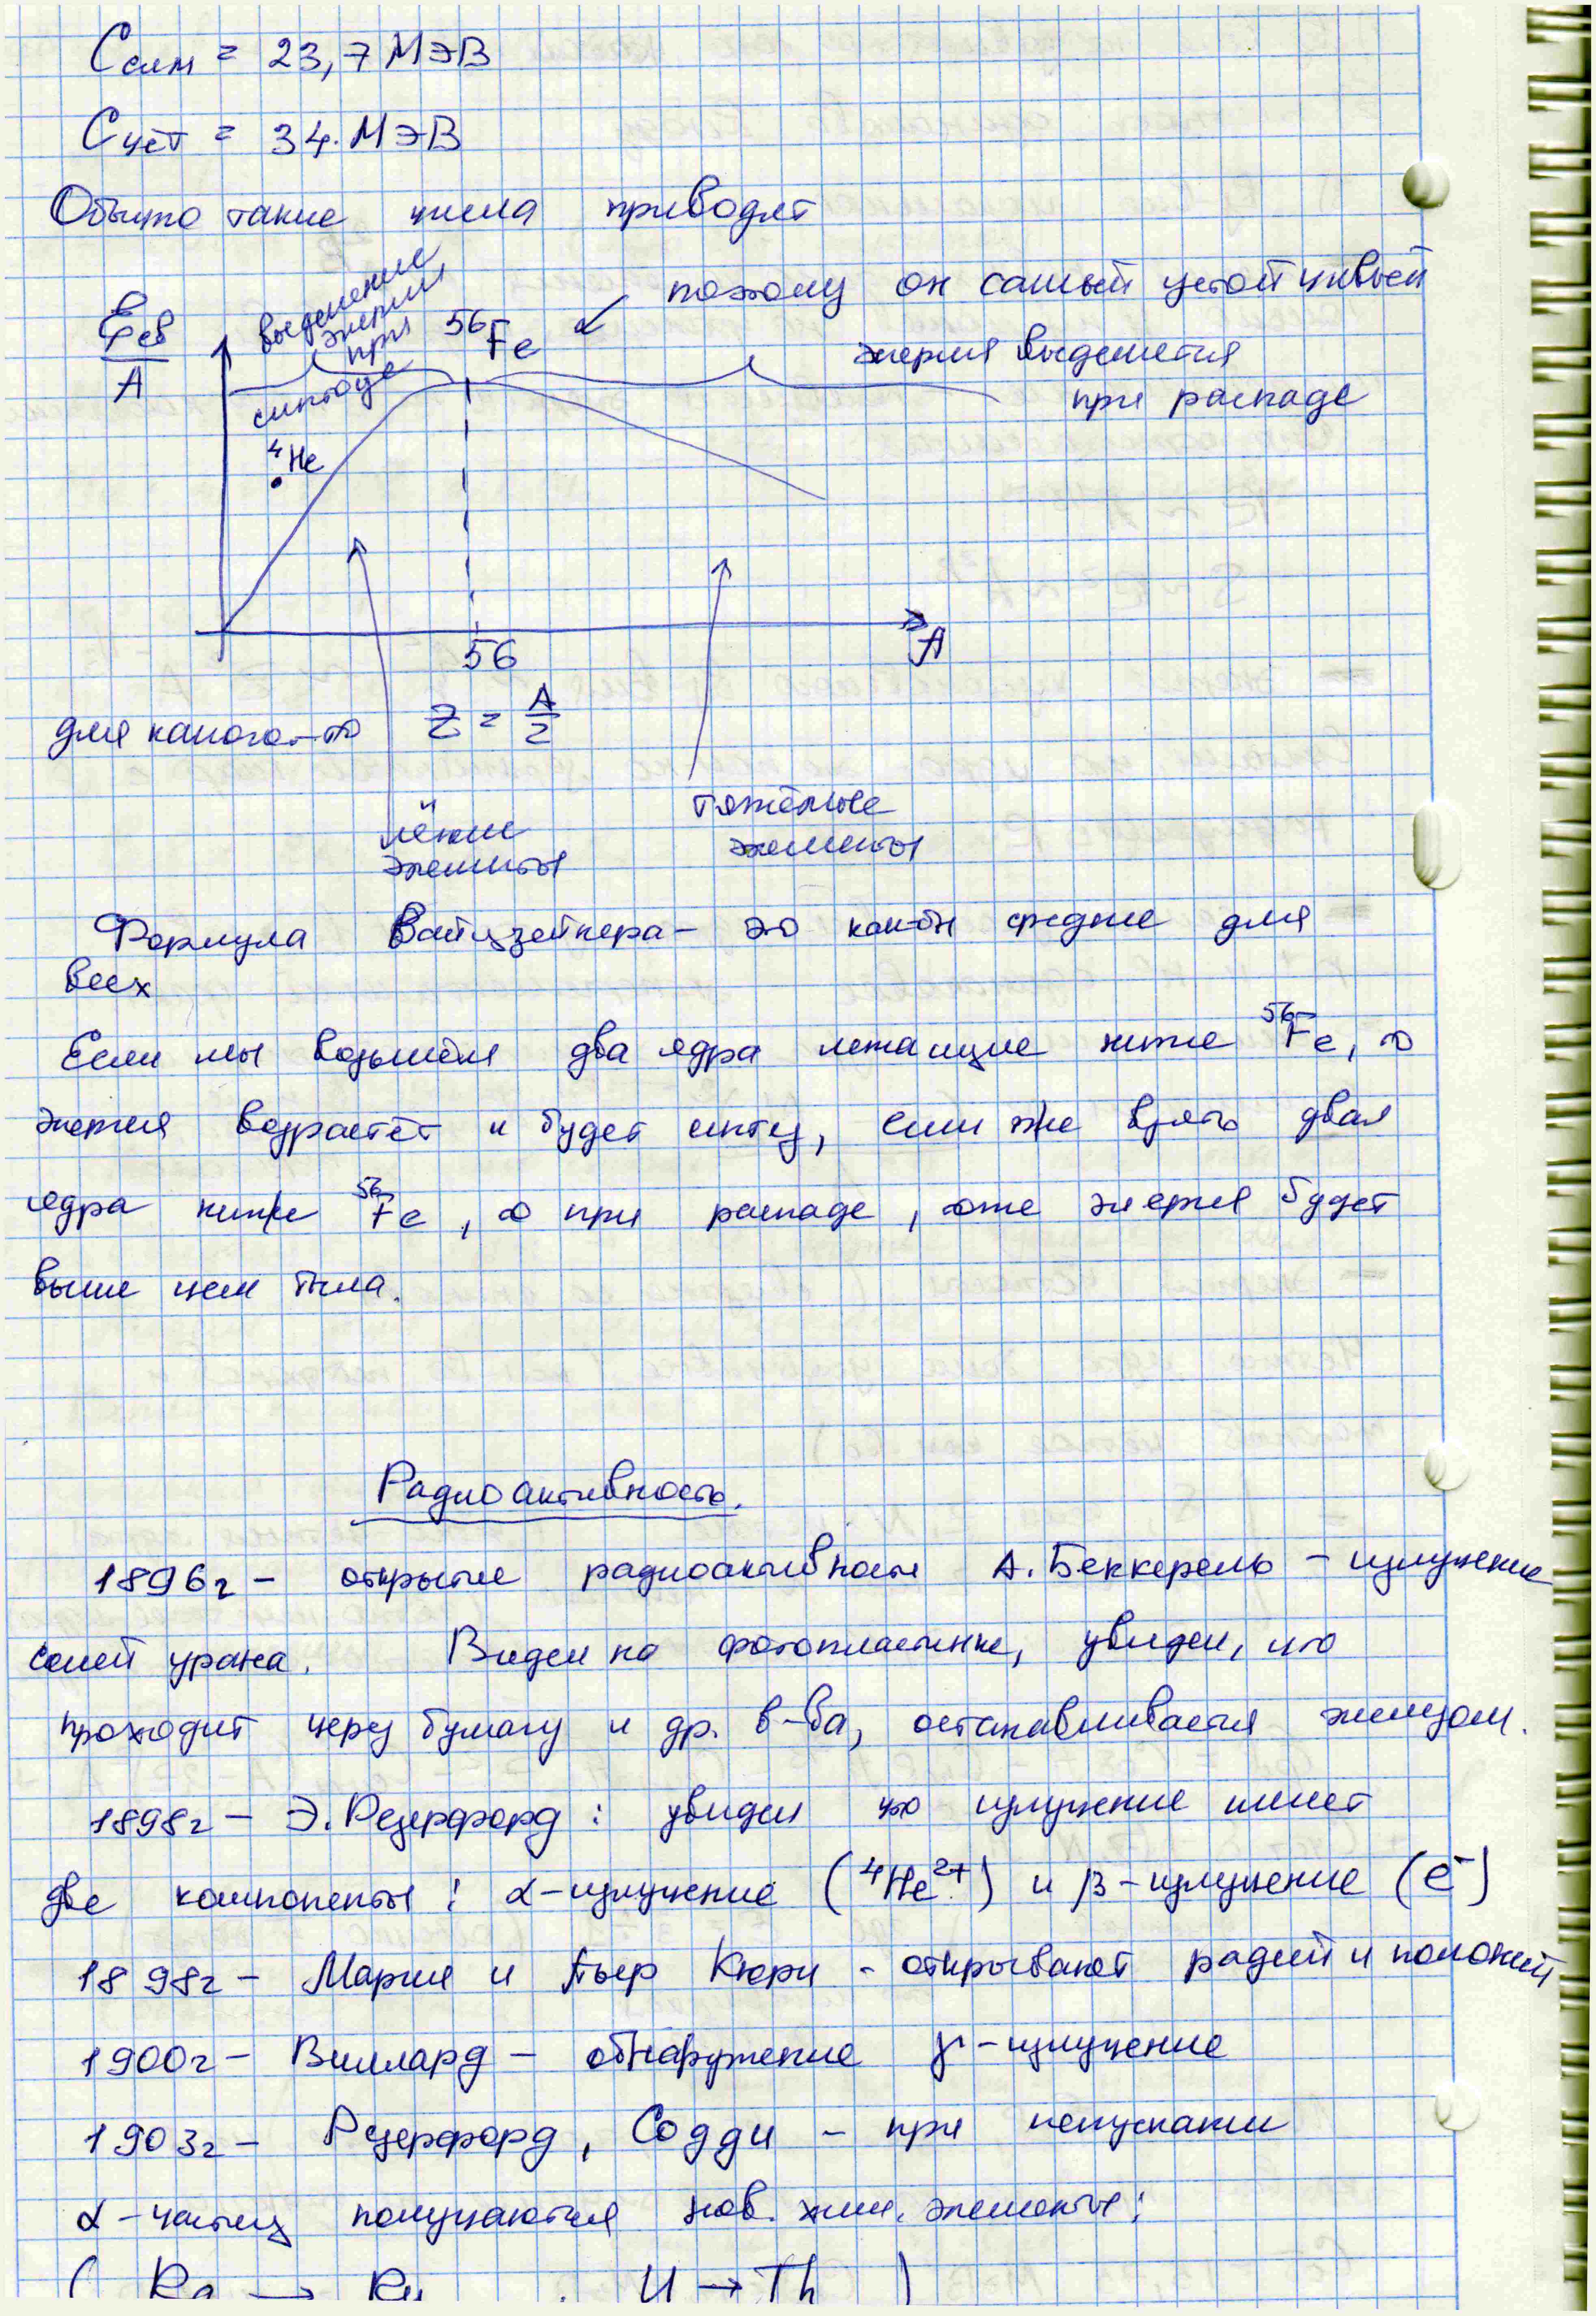
\includegraphics[max size={\textwidth}{0.995\textheight}]{jpg/49.jpg}%
\newpage%
%
\phantomsection\addcontentsline{toc}{subsubsection}{Типы радиоактивных распадов}%
\phantomsection\addcontentsline{toc}{subsubsection}{Закон радиоактивного распада}%
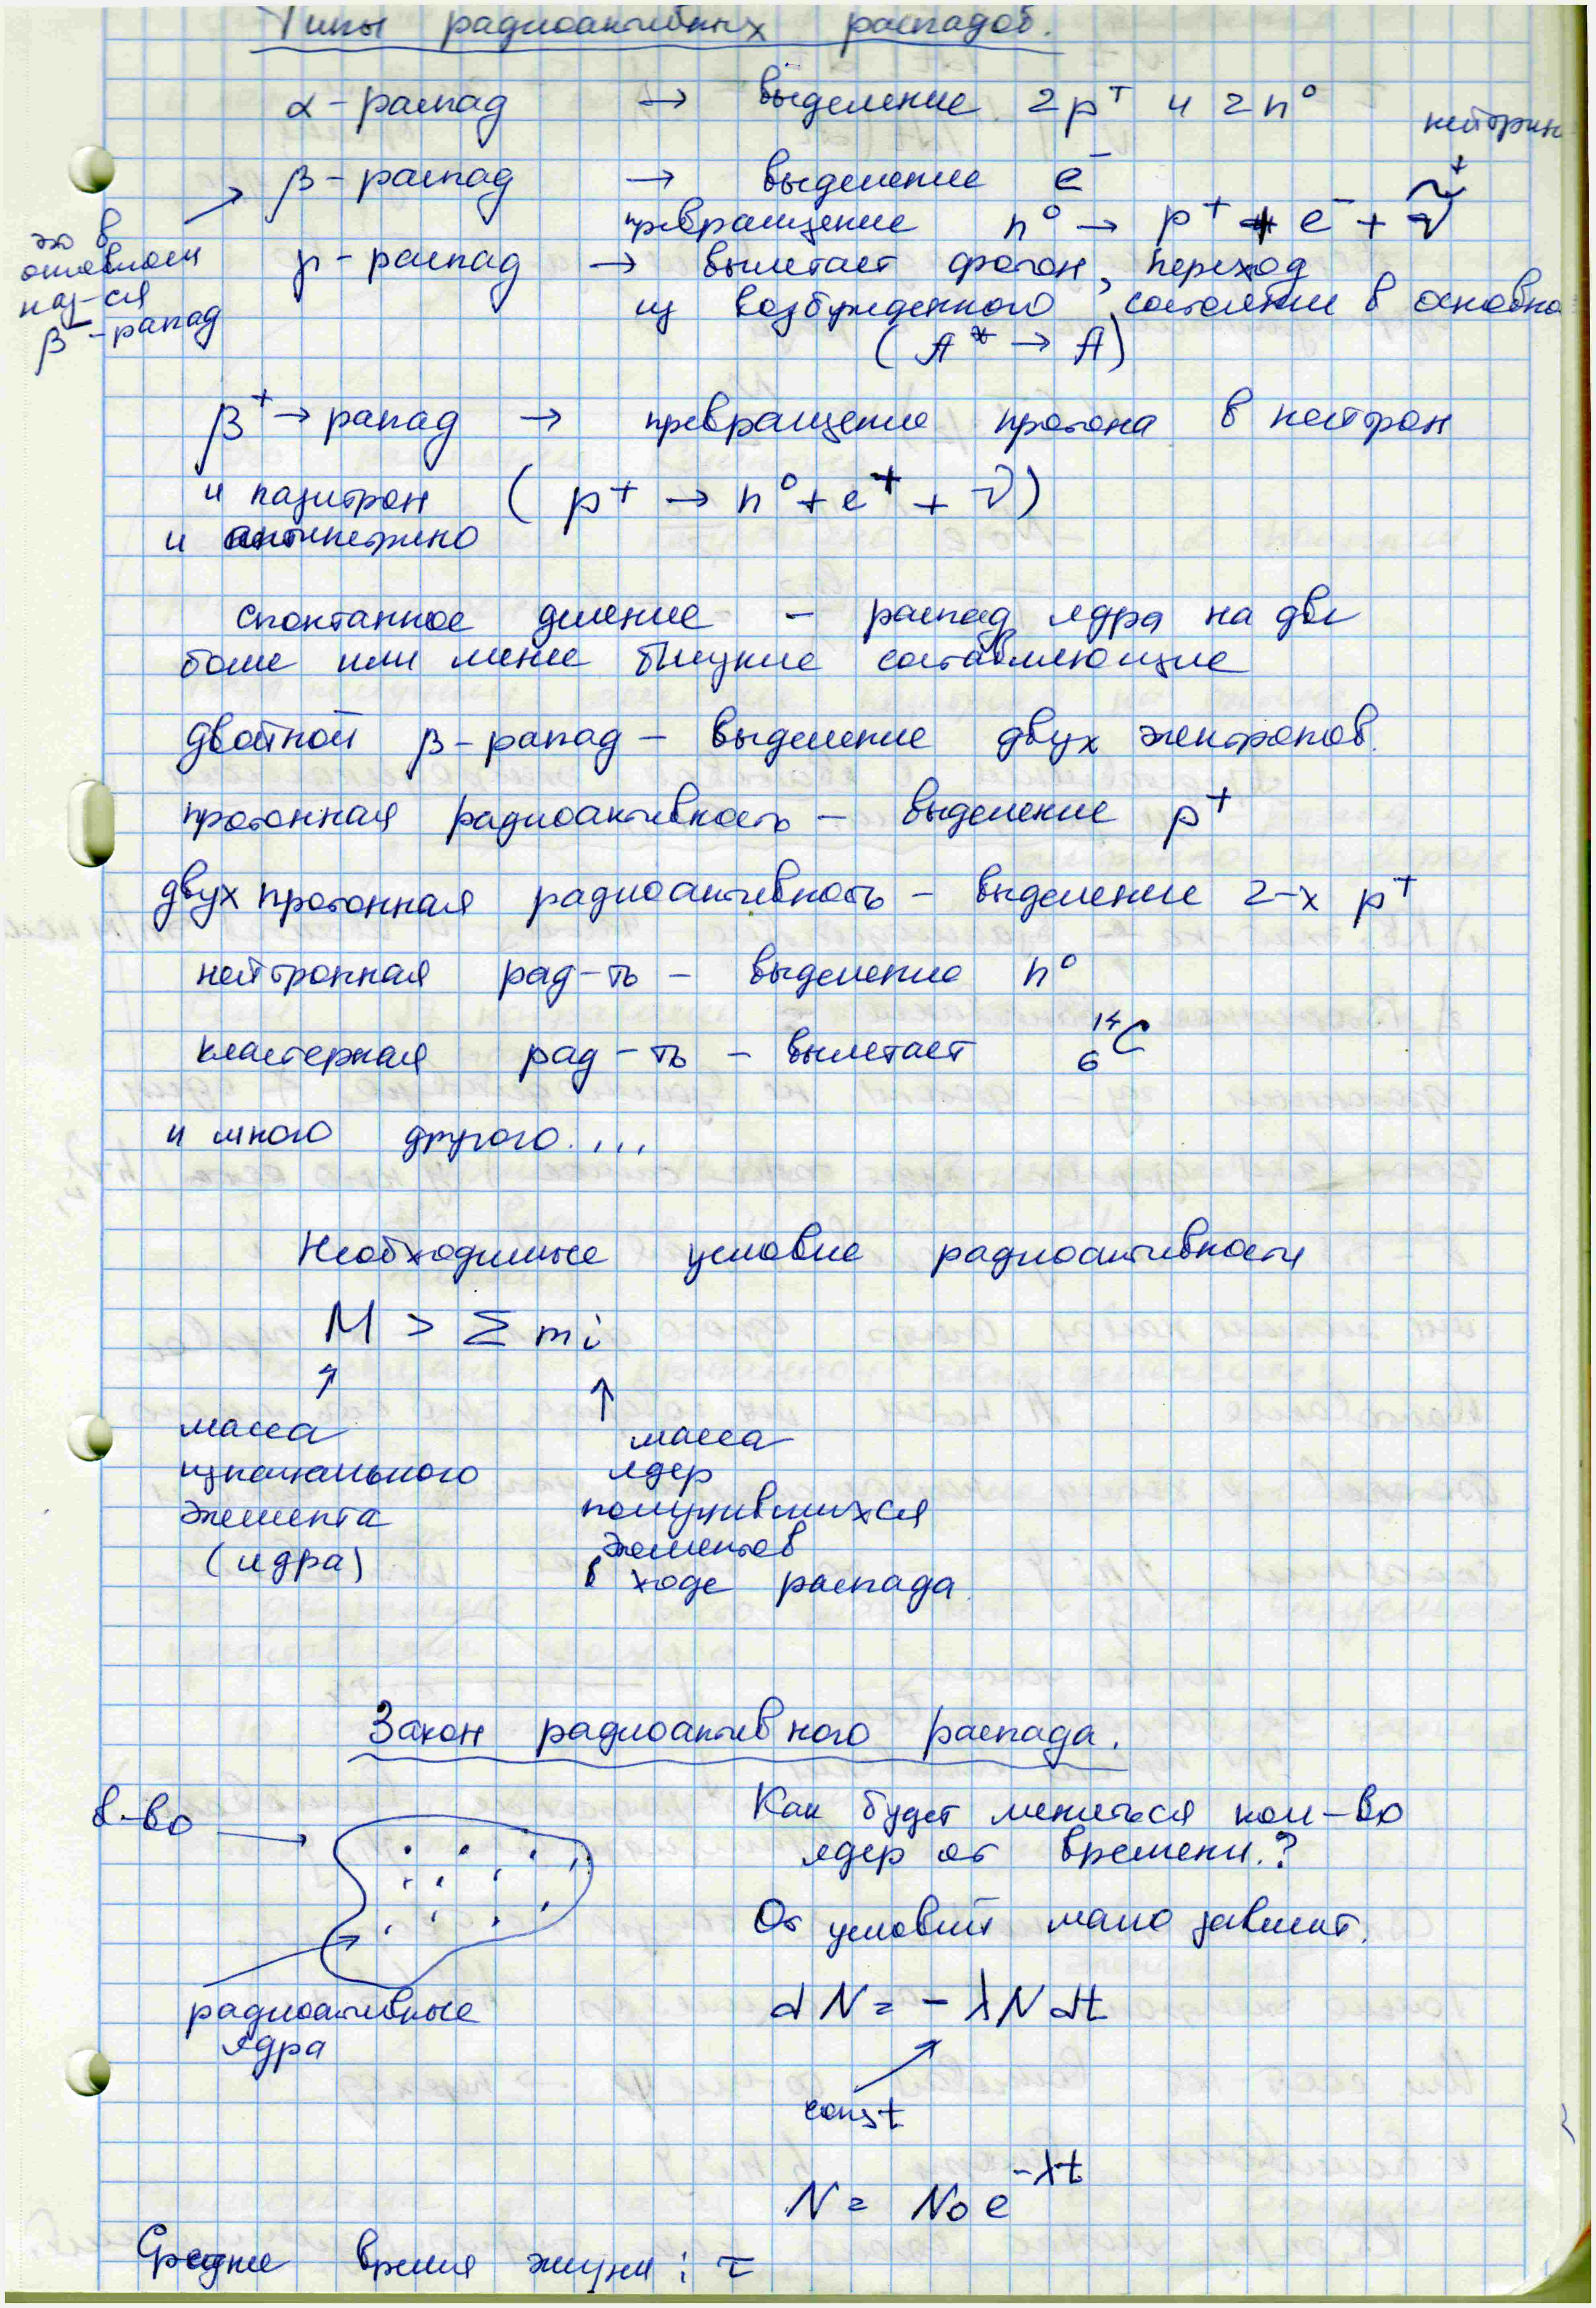
\includegraphics[max size={\textwidth}{0.995\textheight}]{jpg/50.jpg}%
\newpage%
%
\phantomsection\addcontentsline{toc}{section}{\textit{Элементарные частицы}}%
\phantomsection\addcontentsline{toc}{subsection}{Представление о квантовой электродинамике и диаграммы Фейнмана}%
\includegraphics[max size={\textwidth}{0.995\textheight}]{jpg/51.jpg}%
\newpage%
%
%
\includegraphics[max size={\textwidth}{0.995\textheight}]{jpg/52.jpg}%
\newpage%
%
\phantomsection\addcontentsline{toc}{subsection}{Сильное ядерное взаимодействие}%
\includegraphics[max size={\textwidth}{0.995\textheight}]{jpg/53.jpg}%
\newpage%
%
\phantomsection\addcontentsline{toc}{subsection}{Изотопический спин}%
\includegraphics[max size={\textwidth}{0.995\textheight}]{jpg/54.jpg}%
\newpage%
%
\phantomsection\addcontentsline{toc}{subsection}{Странные частицы}%
\includegraphics[max size={\textwidth}{0.995\textheight}]{jpg/55.jpg}%
\newpage%
%
\phantomsection\addcontentsline{toc}{subsection}{Кварки}%
\includegraphics[max size={\textwidth}{0.995\textheight}]{jpg/56.jpg}%
\newpage%
%
%
\includegraphics[max size={\textwidth}{0.995\textheight}]{jpg/57.jpg}%
\newpage%
%
%
\includegraphics[max size={\textwidth}{0.995\textheight}]{jpg/58.jpg}%
\newpage%
%
\phantomsection\addcontentsline{toc}{subsection}{Конфайниент}%
\includegraphics[max size={\textwidth}{0.995\textheight}]{jpg/59.jpg}%
\newpage%
%
\phantomsection\addcontentsline{toc}{subsection}{Слабое ядерное взаимодействие}%
\includegraphics[max size={\textwidth}{0.995\textheight}]{jpg/60.jpg}%
\newpage%
%
%
\includegraphics[max size={\textwidth}{0.995\textheight}]{jpg/61.jpg}%
\newpage%
%
\phantomsection\addcontentsline{toc}{subsection}{Нейтрино}%
\includegraphics[max size={\textwidth}{0.995\textheight}]{jpg/62.jpg}%
\newpage%
%
%
\includegraphics[max size={\textwidth}{0.995\textheight}]{jpg/63.jpg}%
\newpage%
%
%
\includegraphics[max size={\textwidth}{0.995\textheight}]{jpg/64.jpg}%
\newpage%
%
\phantomsection\addcontentsline{toc}{subsection}{Бозон Хиггса}%
\includegraphics[max size={\textwidth}{0.995\textheight}]{jpg/65.jpg}%
\newpage%
%
\phantomsection\addcontentsline{toc}{subsection}{Стандартная модель. Темное вещество}%
\includegraphics[max size={\textwidth}{0.995\textheight}]{jpg/66.jpg}%
\newpage%
%
\phantomsection\addcontentsline{toc}{subsection}{Классификация элементарных частиц}%
\includegraphics[max size={\textwidth}{0.995\textheight}]{jpg/67.jpg}%
\newpage%
%
\phantomsection\addcontentsline{toc}{subsection}{Фундаментальное взаимодействие}%
\includegraphics[max size={\textwidth}{0.995\textheight}]{jpg/68.jpg}%
\newpage%
%
\phantomsection\addcontentsline{toc}{subsection}{Законы сохранения}%
\includegraphics[max size={\textwidth}{0.995\textheight}]{jpg/69.jpg}%
\newpage%
%
%
\includegraphics[max size={\textwidth}{0.995\textheight}]{jpg/70.jpg}%
\newpage%
%
\phantomsection\addcontentsline{toc}{subsection}{За пределами стандартной модели}%
\includegraphics[max size={\textwidth}{0.995\textheight}]{jpg/71.jpg}%
\newpage%
%
\phantomsection\addcontentsline{toc}{subsection}{Квантовая теория гравитации}%
\includegraphics[max size={\textwidth}{0.995\textheight}]{jpg/72.jpg}%
\newpage%
%
%
\includegraphics[max size={\textwidth}{0.995\textheight}]{jpg/73.jpg}%
\newpage%
%
%
\end{document}